% -*- mode: Latex; fill-column: 120; -*-
\documentclass{article}\usepackage[]{graphicx}\usepackage[]{color}
%% maxwidth is the original width if it is less than linewidth
%% otherwise use linewidth (to make sure the graphics do not exceed the margin)
\makeatletter
\def\maxwidth{ %
  \ifdim\Gin@nat@width>\linewidth
    \linewidth
  \else
    \Gin@nat@width
  \fi
}
\makeatother

\definecolor{fgcolor}{rgb}{0.345, 0.345, 0.345}
\newcommand{\hlnum}[1]{\textcolor[rgb]{0.686,0.059,0.569}{#1}}%
\newcommand{\hlstr}[1]{\textcolor[rgb]{0.192,0.494,0.8}{#1}}%
\newcommand{\hlcom}[1]{\textcolor[rgb]{0.678,0.584,0.686}{\textit{#1}}}%
\newcommand{\hlopt}[1]{\textcolor[rgb]{0,0,0}{#1}}%
\newcommand{\hlstd}[1]{\textcolor[rgb]{0.345,0.345,0.345}{#1}}%
\newcommand{\hlkwa}[1]{\textcolor[rgb]{0.161,0.373,0.58}{\textbf{#1}}}%
\newcommand{\hlkwb}[1]{\textcolor[rgb]{0.69,0.353,0.396}{#1}}%
\newcommand{\hlkwc}[1]{\textcolor[rgb]{0.333,0.667,0.333}{#1}}%
\newcommand{\hlkwd}[1]{\textcolor[rgb]{0.737,0.353,0.396}{\textbf{#1}}}%
\let\hlipl\hlkwb

\usepackage{framed}
\makeatletter
\newenvironment{kframe}{%
 \def\at@end@of@kframe{}%
 \ifinner\ifhmode%
  \def\at@end@of@kframe{\end{minipage}}%
  \begin{minipage}{\columnwidth}%
 \fi\fi%
 \def\FrameCommand##1{\hskip\@totalleftmargin \hskip-\fboxsep
 \colorbox{shadecolor}{##1}\hskip-\fboxsep
     % There is no \\@totalrightmargin, so:
     \hskip-\linewidth \hskip-\@totalleftmargin \hskip\columnwidth}%
 \MakeFramed {\advance\hsize-\width
   \@totalleftmargin\z@ \linewidth\hsize
   \@setminipage}}%
 {\par\unskip\endMakeFramed%
 \at@end@of@kframe}
\makeatother

\definecolor{shadecolor}{rgb}{.97, .97, .97}
\definecolor{messagecolor}{rgb}{0, 0, 0}
\definecolor{warningcolor}{rgb}{1, 0, 1}
\definecolor{errorcolor}{rgb}{1, 0, 0}
\newenvironment{knitrout}{}{} % an empty environment to be redefined in TeX

\usepackage{alltt}

\usepackage[letterpaper,margin=1in]{geometry}
\usepackage[breaklinks=true,colorlinks=true,urlcolor=blue]{hyperref}
\usepackage{bookmark}
\usepackage{times}
\usepackage{amsmath}
%\usepackage{graphicx}\usepackage[]{color}  knitr adds these
\IfFileExists{upquote.sty}{\usepackage{upquote}}{}
\begin{document}
\title{Time-In-Culture Analysis}
\maketitle

\tableofcontents

\section{Intro}
More stream-of-consciousness analysis, focused (euphemistically speaking) on Time-In-Culture effects, especially hemizygosity.

\section{Preliminaries}
Load utility R code; do setup:

% setup.my.knitr includes opts_chunk$set(size='footnotesize'), but needed 1st time.
\begin{knitrout}\footnotesize
\definecolor{shadecolor}{rgb}{0.969, 0.969, 0.969}\color{fgcolor}\begin{kframe}
\begin{alltt}
\hlkwd{source}\hlstd{(}\hlstr{'../../../R/wlr.R'}\hlstd{)} \hlcom{# load util code; path relative this folder or sibling in scripts/larrys }
\end{alltt}
\begin{verbatim}
## Running as: ruzzo @ ruzzo.local; SVN Id, I miss you.  $Id: wlr.R  2017-06-26 or later $
\end{verbatim}
\begin{alltt}
\hlkwd{setup.my.wd}\hlstd{(}\hlstr{'tic'}\hlstd{)}         \hlcom{# set working dir; UPDATE if this file moves, or if COPY/PASTE to new file}
\hlkwd{setup.my.knitr}\hlstd{(}\hlstr{'figs-knitr/'}\hlstd{)}
\hlstd{my.figs.dir} \hlkwb{<-} \hlstr{'figs-mine/'}
\hlkwd{generic.setup}\hlstd{(my.figs.dir)}            \hlcom{# Create figs dir etc., if needed.}
\hlcom{# some more params for knitr}
\hlkwa{if}\hlstd{(}\hlkwd{exists}\hlstd{(}\hlstr{'opts_knit'}\hlstd{))\{}
  \hlcom{# If knitr is loaded, set some of its options.  }
  \hlcom{# (Skip if not loaded, e.g., when playing in Rstudio.)}
  \hlstd{opts_chunk}\hlopt{$}\hlkwd{set}\hlstd{(}\hlkwc{fig.align}\hlstd{=}\hlstr{'center'}\hlstd{,}\hlkwc{fig.show}\hlstd{=}\hlstr{'hold'}\hlstd{,}\hlkwc{fig.pos}\hlstd{=}\hlstr{'tp'}\hlstd{)}
  \hlstd{opts_knit}\hlopt{$}\hlkwd{set}\hlstd{(}\hlkwc{eval.after}\hlstd{=}\hlstr{'fig.cap'}\hlstd{)} \hlcom{## so fig caption can be built using values from the code }
  \hlcom{# opts_knit$set(width=1350) # width=85 in setup.my.knitr; do we want to override it?}
\hlstd{\}}
\end{alltt}
\end{kframe}
\end{knitrout}

\iffalse
% latex font sizes: \tiny \scriptsize \footnotesize \small \normalsize \large \Large \LARGE \huge \Huge
\begin{knitrout}\footnotesize
\definecolor{shadecolor}{rgb}{0.969, 0.969, 0.969}\color{fgcolor}\begin{kframe}
\begin{alltt}
\hlcom{# attempt to calibrate print width in footnotesize (this chunk) and scriptsize, tiny (next 2)}
\hlcom{#        1         2         3         4         5         6         7         8         9         A}
\hlcom{#234567890123456789012345678901234567890123456789012345678901234567890123456789012345678901234567890}
\end{alltt}
\end{kframe}
\end{knitrout}

\begin{knitrout}\scriptsize
\definecolor{shadecolor}{rgb}{0.969, 0.969, 0.969}\color{fgcolor}\begin{kframe}
\begin{alltt}
\hlcom{#        1         2         3         4         5         6         7         8         9         A         B}
\hlcom{#2345678901234567890123456789012345678901234567890123456789012345678901234567890123456789012345678901234567890}
\end{alltt}
\end{kframe}
\end{knitrout}

\begin{knitrout}\tiny
\definecolor{shadecolor}{rgb}{0.969, 0.969, 0.969}\color{fgcolor}\begin{kframe}
\begin{alltt}
\hlcom{#        1         2         3         4         5         6         7         8         9         A         B         C         D         E         F         G}
\hlcom{#234567890123456789012345678901234567890123456789012345678901234567890123456789012345678901234567890123456789012345678901234567890123456789012345678901234567890}
\end{alltt}
\end{kframe}
\end{knitrout}
\fi

% Also load the desert tables, in case needed:

\begin{knitrout}\footnotesize
\definecolor{shadecolor}{rgb}{0.969, 0.969, 0.969}\color{fgcolor}\begin{kframe}
\begin{alltt}
\hlcom{# from svn+ssh://ceg1.ocean.washington.edu/var/svn/7_strains/trunk/code/snpNB/data}
\hlcom{# load('../../../data/des.rda')}
\end{alltt}
\end{kframe}
\end{knitrout}

\section{CNVnator Analysis}

Load Chris' CNVnator output file.  The 4 paths below are 
(1) Larry's old path within the svn tree; 
(2) newer one within git tree; 
(3) the same, but relative to current dir; and 
(4) local dir. 
I decided to put a symlink in the local dir with that name, linked to the real file via path3;
I think this will make it more obvious what to change should we ever reoranize the tree.

\begin{knitrout}\footnotesize
\definecolor{shadecolor}{rgb}{0.969, 0.969, 0.969}\color{fgcolor}\begin{kframe}
\begin{alltt}
\hlkwd{getwd}\hlstd{()} \hlcom{## just to be sure it's set correctly}
\end{alltt}
\begin{verbatim}
# [1] "/Users/ruzzo/Documents/g/projects/thaps/Thaps_7_strains/code/snpNB/scripts/larrys/tic"
\end{verbatim}
\begin{alltt}
\hlcom{#cnv.path1 <- '/Users/ruzzo/Documents/s/papers/Thaps/chris/cnv.txt'}
\hlcom{#cnv.path2 <- '/Users/ruzzo/Documents/g/projects/thaps/Thaps_7_strains/code/snpNB/data/cnv.txt'}
\hlcom{#cnv.path3 <- '../../../data/cnv.txt'}
\hlstd{cnv.path} \hlkwb{<-} \hlstr{'cnv.txt'}  \hlcom{## should be a symlink in tic directory to the CNVnator output}
\hlstd{cnv} \hlkwb{<-} \hlkwd{read.delim}\hlstd{(cnv.path)}
\end{alltt}
\end{kframe}
\end{knitrout}

Check for/correct oddities:

\begin{knitrout}\footnotesize
\definecolor{shadecolor}{rgb}{0.969, 0.969, 0.969}\color{fgcolor}\begin{kframe}
\begin{alltt}
\hlkwd{str}\hlstd{(cnv)}
\end{alltt}
\begin{verbatim}
# 'data.frame':	2380 obs. of  9 variables:
#  $ strain   : Factor w/ 7 levels "IT","tp1007",..: 3 3 3 3 3 3 3 3 3 3 ...
#  $ chr      : Factor w/ 65 levels "BD1_7","BD10_65",..: 38 38 38 38 38 38 38 38 38 38 ...
#  $ start    : int  10601 112001 215001 358901 536501 554801 673401 781801 806901 853201 ...
#  $ end      : int  13500 116500 221100 370300 538600 559300 685000 787400 811100 855600 ...
#  $ length   : int  2900 4500 6100 11400 2100 4500 11600 5600 4200 2400 ...
#  $ filtered : Factor w/ 2 levels "False","True": 1 1 1 2 1 1 1 1 1 1 ...
#  $ type     : Factor w/ 1 level "CNVnator": 1 1 1 1 1 1 1 1 1 1 ...
#  $ cov_ratio: num  0.63738 1.54893 1.65381 0.00204 0.68486 ...
#  $ dup_frac : num  0.41188 0.00908 0.01178 0.97997 0.0211 ...
\end{verbatim}
\begin{alltt}
\hlstd{cnv[}\hlkwd{c}\hlstd{(}\hlnum{1}\hlopt{:}\hlnum{4}\hlstd{,}\hlnum{2378}\hlopt{:}\hlnum{2380}\hlstd{),]}
\end{alltt}
\begin{verbatim}
#      strain     chr  start    end length filtered     type  cov_ratio   dup_frac
# 1    tp1012    Chr1  10601  13500   2900    False CNVnator 0.63738000 0.41187900
# 2    tp1012    Chr1 112001 116500   4500    False CNVnator 1.54893000 0.00907677
# 3    tp1012    Chr1 215001 221100   6100    False CNVnator 1.65381000 0.01178470
# 4    tp1012    Chr1 358901 370300  11400     True CNVnator 0.00204431 0.97997300
# 2378 tp1335 BD36_69   6201  11900   5700    False CNVnator 4.86642000 0.94409000
# 2379 tp1335 BD36_69  12001  17900   5900    False CNVnator 1.16742000 0.85396800
# 2380 tp1335 BD37_91      1  13900  13900     True CNVnator 0.67417500 0.53919900
\end{verbatim}
\begin{alltt}
\hlstd{cnv}\hlopt{$}\hlstd{filtered} \hlkwb{<-} \hlstd{cnv}\hlopt{$}\hlstd{filtered} \hlopt{==} \hlstr{'True'}     \hlcom{## convert factor to Bool}
\hlkwd{all}\hlstd{(cnv}\hlopt{$}\hlstd{length} \hlopt{==} \hlstd{(cnv}\hlopt{$}\hlstd{end}\hlopt{-}\hlstd{cnv}\hlopt{$}\hlstd{start}\hlopt{+}\hlnum{1}\hlstd{))}   \hlcom{## start/end/length as expected}
\end{alltt}
\begin{verbatim}
# [1] TRUE
\end{verbatim}
\begin{alltt}
\hlkwa{for}\hlstd{(i} \hlkwa{in} \hlnum{1}\hlopt{:}\hlnum{9}\hlstd{)\{}
  \hlkwa{if}\hlstd{(}\hlkwd{any}\hlstd{(}\hlkwd{is.na}\hlstd{(cnv[,i])))\{}
    \hlkwd{cat}\hlstd{(}\hlstr{'NA in column'}\hlstd{,i,}\hlstr{'\textbackslash{}n'}\hlstd{)}
  \hlstd{\}}
\hlstd{\}}
\hlstd{strain.names} \hlkwb{<-} \hlkwd{c}\hlstd{(}\hlkwd{paste}\hlstd{(}\hlstr{'tp10'}\hlstd{,}\hlkwd{c}\hlstd{(}\hlstr{'07'}\hlstd{,}\hlnum{12}\hlopt{:}\hlnum{15}\hlstd{),}\hlkwc{sep}\hlstd{=}\hlstr{''}\hlstd{),}\hlstr{'IT'}\hlstd{,}\hlstr{'tp1335'}\hlstd{)} \hlcom{# old-school names; IT = 3367}
\hlkwd{rbind}\hlstd{(}\hlkwd{sort}\hlstd{(strain.names),}\hlkwd{levels}\hlstd{(cnv}\hlopt{$}\hlstd{strain))}
\end{alltt}
\begin{verbatim}
#      [,1] [,2]     [,3]     [,4]     [,5]     [,6]     [,7]    
# [1,] "IT" "tp1007" "tp1012" "tp1013" "tp1014" "tp1015" "tp1335"
# [2,] "IT" "tp1007" "tp1012" "tp1013" "tp1014" "tp1015" "tp1335"
\end{verbatim}
\end{kframe}
\end{knitrout}

Some simple descriptive statistics.  Cov ratios near 1 are expected, not called, but lots of stuff below 0.8 and above 1.2: 

\begin{knitrout}\footnotesize
\definecolor{shadecolor}{rgb}{0.969, 0.969, 0.969}\color{fgcolor}\begin{kframe}
\begin{alltt}
\hlkwd{hist}\hlstd{(cnv}\hlopt{$}\hlstd{cov_ratio,}\hlkwc{breaks}\hlstd{=}\hlnum{0}\hlopt{:}\hlnum{120}\hlopt{/}\hlnum{10}\hlstd{)}
\end{alltt}
\end{kframe}

{\centering 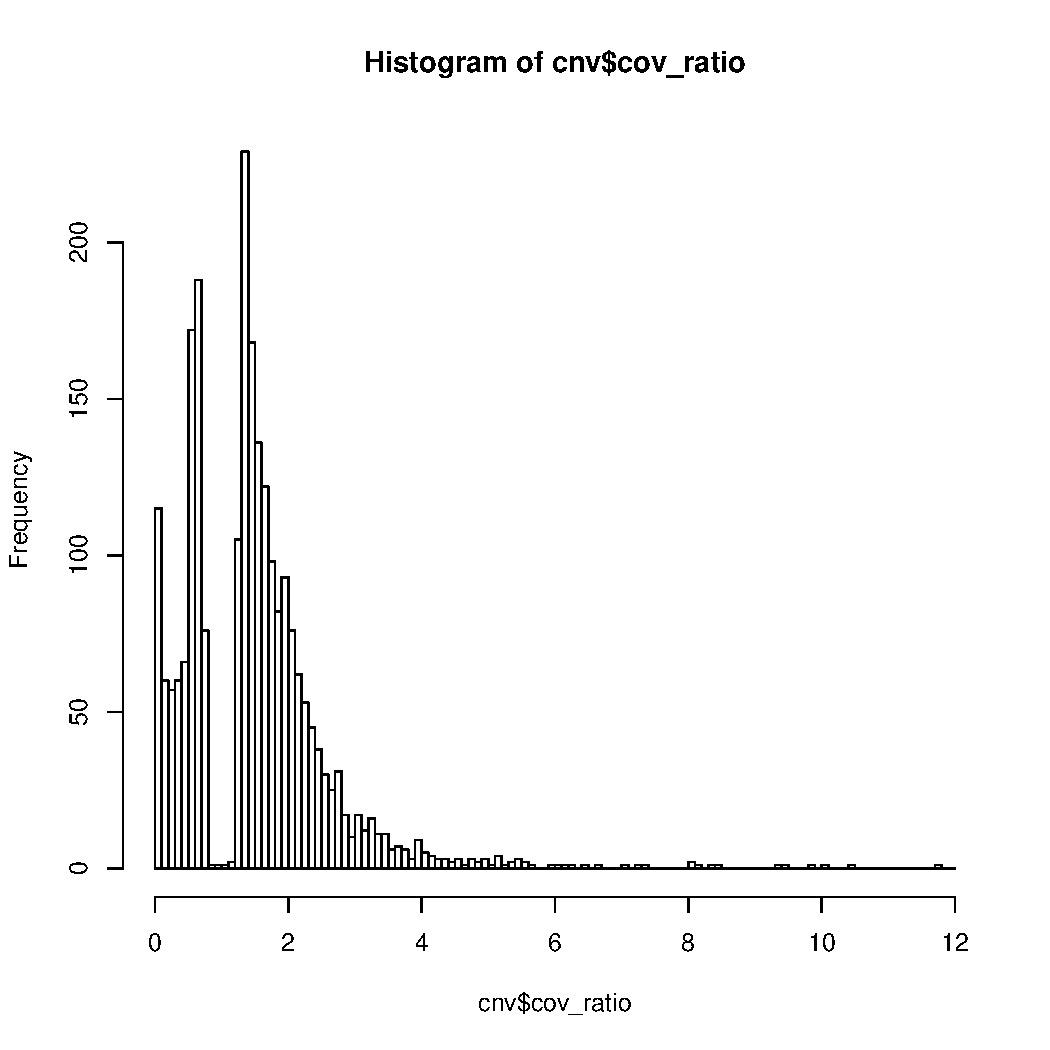
\includegraphics[width=\maxwidth]{figs-knitr/unnamed-chunk-8-1} 

}



\end{knitrout}

What does "Filtered" column mean?  It correlates to \verb|dup_frac|, but loosely:

\begin{knitrout}\footnotesize
\definecolor{shadecolor}{rgb}{0.969, 0.969, 0.969}\color{fgcolor}\begin{kframe}
\begin{alltt}
\hlkwd{hist}\hlstd{(cnv}\hlopt{$}\hlstd{dup_frac,}\hlkwc{breaks}\hlstd{=}\hlnum{0}\hlopt{:}\hlnum{100}\hlopt{/}\hlnum{100}\hlstd{)}
\hlkwd{hist}\hlstd{(cnv}\hlopt{$}\hlstd{dup_frac[}\hlopt{!}\hlstd{cnv}\hlopt{$}\hlstd{filtered],}\hlkwc{breaks}\hlstd{=}\hlnum{0}\hlopt{:}\hlnum{100}\hlopt{/}\hlnum{100}\hlstd{,}\hlkwc{col}\hlstd{=}\hlstr{'blue'}\hlstd{,}\hlkwc{add}\hlstd{=T)}
\hlkwd{legend}\hlstd{(}\hlstr{'topright'}\hlstd{,}\hlkwc{legend}\hlstd{=}\hlstr{'blue=non-filtered'}\hlstd{,}\hlkwc{bty}\hlstd{=}\hlstr{'n'}\hlstd{)}
\end{alltt}
\end{kframe}

{\centering 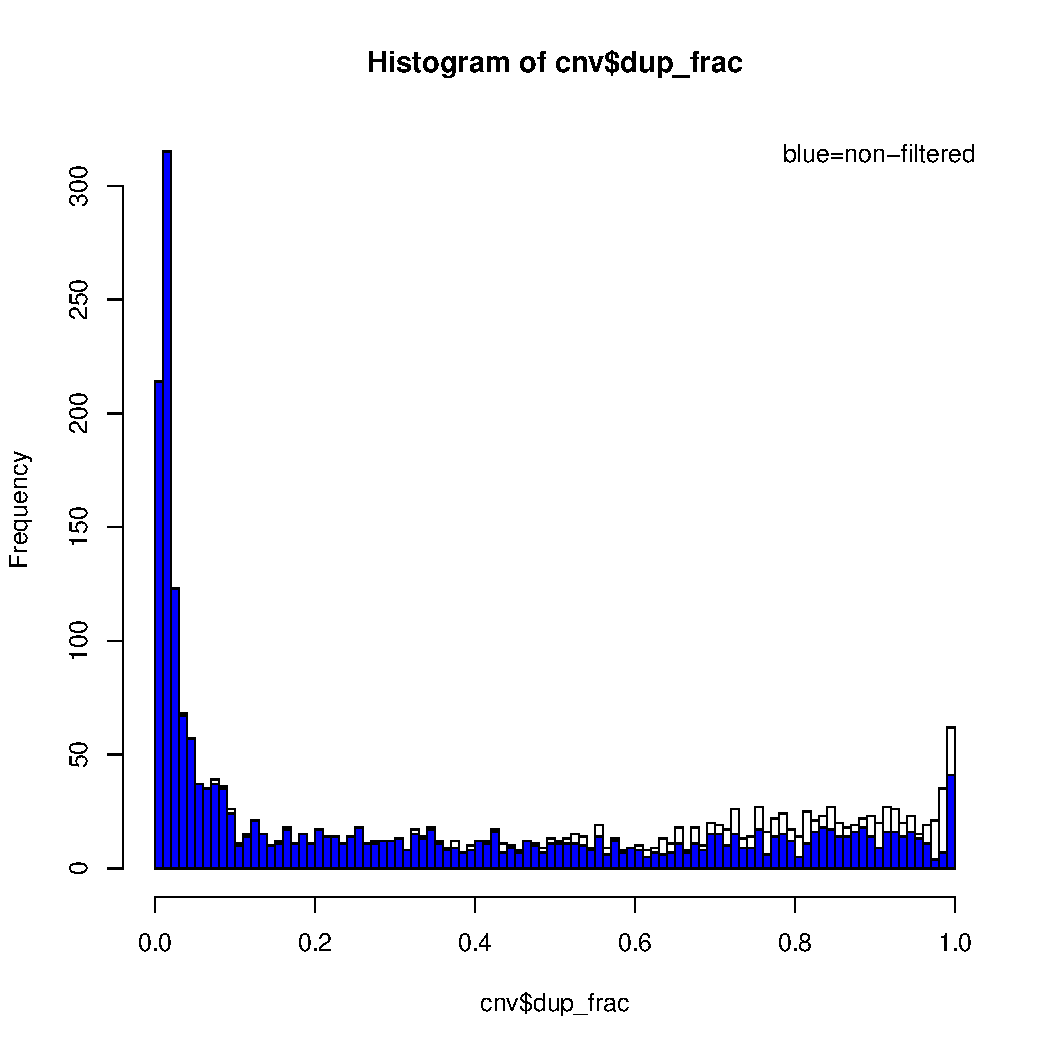
\includegraphics[width=\maxwidth]{figs-knitr/unnamed-chunk-9-1} 

}



\end{knitrout}
\begin{knitrout}\footnotesize
\definecolor{shadecolor}{rgb}{0.969, 0.969, 0.969}\color{fgcolor}\begin{kframe}
\begin{alltt}
\hlkwd{boxplot}\hlstd{(dup_frac} \hlopt{~} \hlstd{filtered,} \hlkwc{data}\hlstd{=cnv,}\hlkwc{ylab}\hlstd{=}\hlstr{'dup_frac'}\hlstd{,} \hlkwc{xlab}\hlstd{=}\hlstr{'filtered'}\hlstd{)}
\end{alltt}
\end{kframe}

{\centering 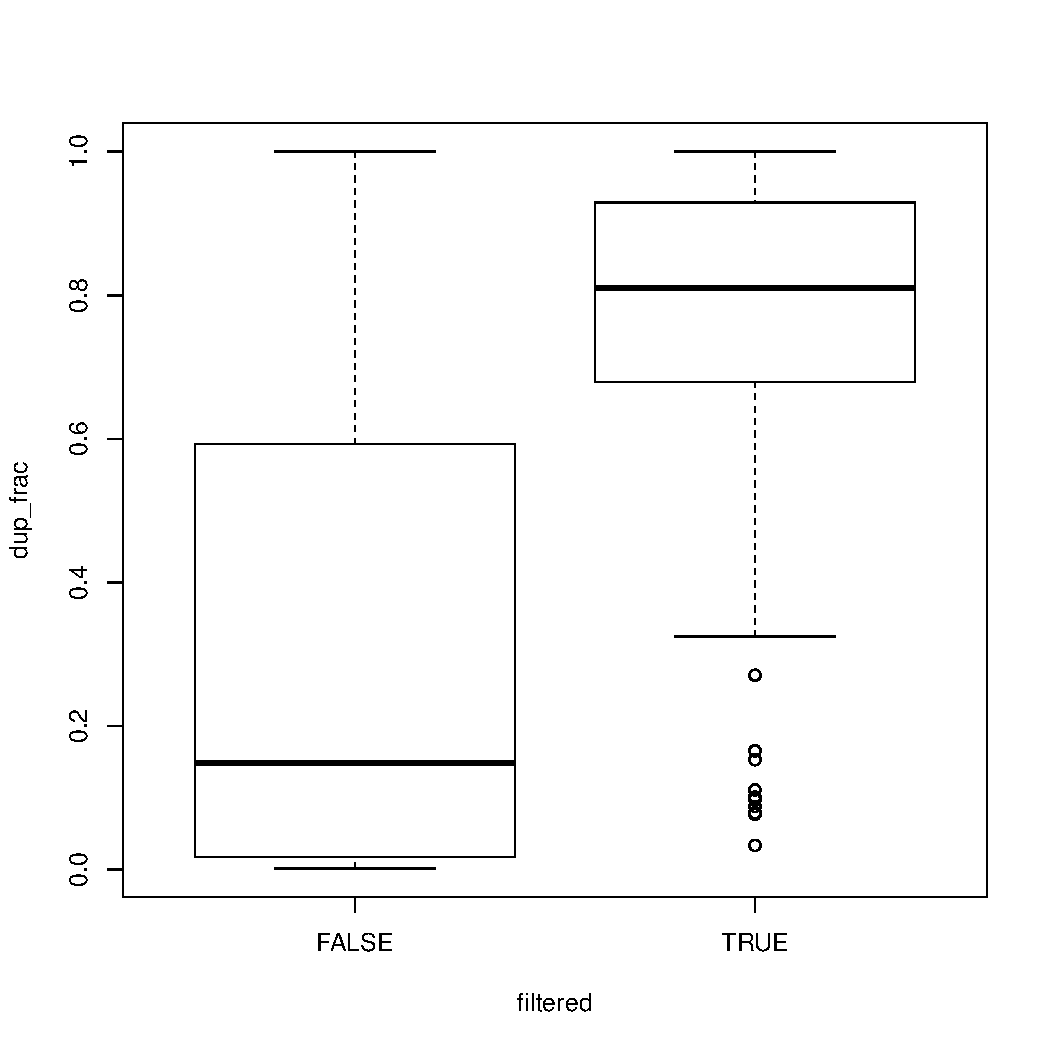
\includegraphics[width=\maxwidth]{figs-knitr/unnamed-chunk-10-1} 

}



\end{knitrout}
\begin{knitrout}\footnotesize
\definecolor{shadecolor}{rgb}{0.969, 0.969, 0.969}\color{fgcolor}\begin{kframe}
\begin{alltt}
\hlkwd{library}\hlstd{(compactr)}
\hlstd{opar} \hlkwb{<-} \hlkwd{par}\hlstd{(}\hlkwc{mfrow}\hlstd{=}\hlkwd{c}\hlstd{(}\hlnum{4}\hlstd{,}\hlnum{2}\hlstd{),}\hlkwc{mar}\hlstd{=}\hlkwd{c}\hlstd{(}\hlnum{0}\hlstd{,}\hlnum{0}\hlstd{,}\hlnum{1}\hlstd{,}\hlnum{.5}\hlstd{),}\hlkwc{oma}\hlstd{=}\hlkwd{c}\hlstd{(}\hlnum{3}\hlstd{,}\hlnum{4}\hlstd{,}\hlnum{1}\hlstd{,}\hlnum{0}\hlstd{))}
\hlstd{thexlim} \hlkwb{<-} \hlkwd{log2}\hlstd{(}\hlnum{1}\hlopt{+}\hlkwd{range}\hlstd{(cnv}\hlopt{$}\hlstd{cov_ratio))}
\hlkwa{for}\hlstd{(st} \hlkwa{in} \hlstd{strain.names)\{}
  \hlkwd{eplot}\hlstd{(}\hlkwc{xlim}\hlstd{=thexlim,} \hlkwc{xlab}\hlstd{=}\hlstr{'log2(1+cov_ratio)'}\hlstd{,} \hlkwc{ylim}\hlstd{=}\hlkwd{c}\hlstd{(}\hlnum{0}\hlstd{,}\hlnum{1}\hlstd{),} \hlkwc{ylab}\hlstd{=}\hlstr{'dup_frac'}\hlstd{,} \hlkwc{main}\hlstd{=st)}
  \hlkwd{points}\hlstd{(dup_frac[strain}\hlopt{==}\hlstd{st]} \hlopt{~} \hlkwd{log2}\hlstd{(}\hlnum{1}\hlopt{+}\hlstd{cov_ratio[strain}\hlopt{==}\hlstd{st]),} \hlkwc{data}\hlstd{=cnv,} \hlkwc{col}\hlstd{=}\hlkwd{ifelse}\hlstd{(filtered,}\hlstr{'black'}\hlstd{,}\hlstr{'blue'}\hlstd{))}
  \hlkwa{if}\hlstd{(st}\hlopt{==}\hlstr{'IT'}\hlstd{)\{}\hlkwd{addxaxis}\hlstd{()\}}
\hlstd{\}}
\hlkwd{plot}\hlstd{(}\hlnum{0}\hlstd{,}\hlnum{0}\hlstd{,}\hlkwc{type}\hlstd{=}\hlstr{'n'}\hlstd{,}\hlkwc{axes}\hlstd{=F,}\hlkwc{frame.plot}\hlstd{=F,}\hlkwc{xlab}\hlstd{=}\hlstr{''}\hlstd{,}\hlkwc{ylab}\hlstd{=}\hlstr{''}\hlstd{)}
\hlkwd{legend}\hlstd{(}\hlstr{'center'}\hlstd{,}\hlkwc{legend}\hlstd{=}\hlstr{'blue=non-filtered'}\hlstd{,}\hlkwc{bty}\hlstd{=}\hlstr{'n'}\hlstd{)}
\hlkwd{par}\hlstd{(opar)}
\end{alltt}
\end{kframe}

{\centering 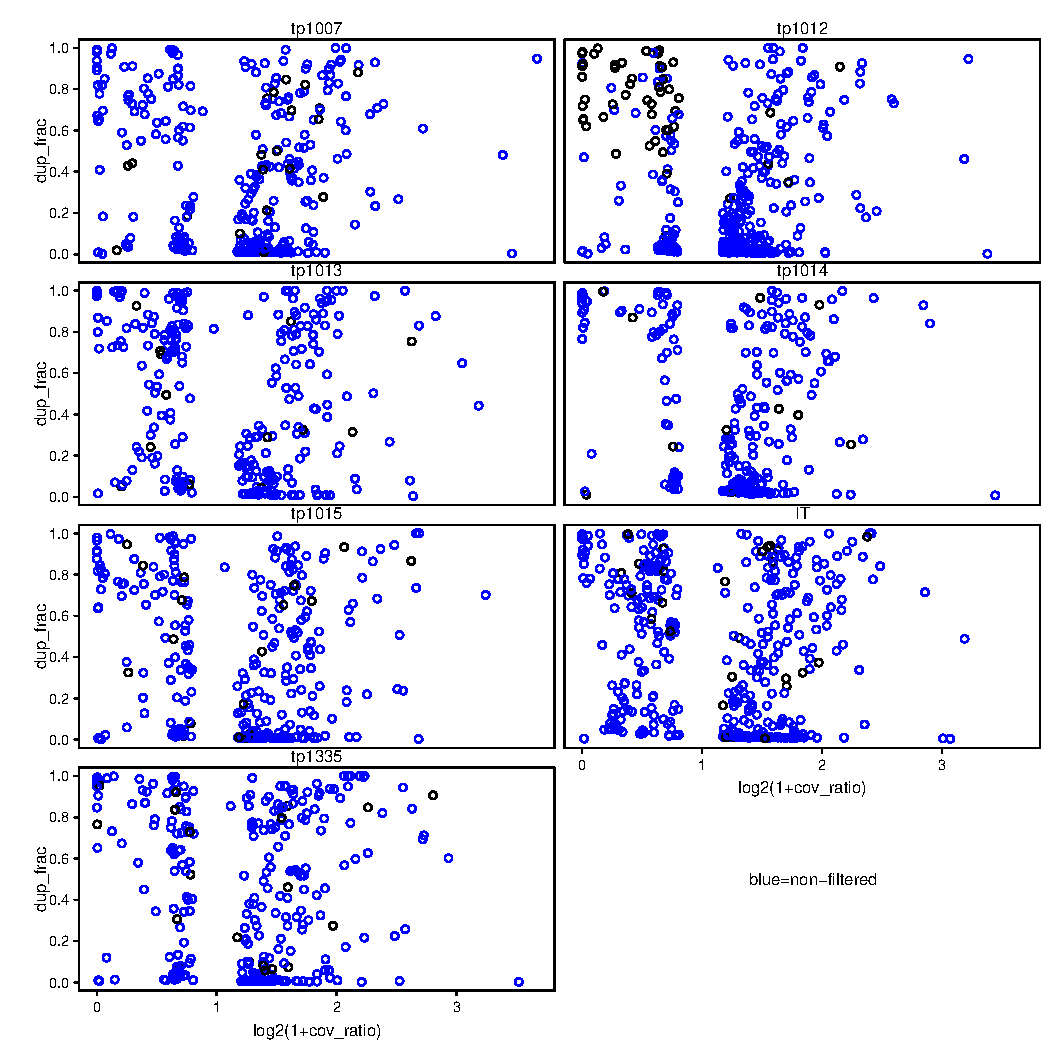
\includegraphics[width=\maxwidth]{figs-knitr/unnamed-chunk-11-1} 

}



\end{knitrout}

Most ``events'' are shorter than 5-10k, but the few big events cover most of the deleted bases.

\begin{knitrout}\footnotesize
\definecolor{shadecolor}{rgb}{0.969, 0.969, 0.969}\color{fgcolor}\begin{kframe}
\begin{alltt}
\hlstd{opar} \hlkwb{<-} \hlkwd{par}\hlstd{(}\hlkwc{mfrow}\hlstd{=}\hlkwd{c}\hlstd{(}\hlnum{1}\hlstd{,}\hlnum{2}\hlstd{))}
\hlkwd{hist}\hlstd{(}\hlkwd{log2}\hlstd{(cnv}\hlopt{$}\hlstd{length))}
\hlstd{sl} \hlkwb{<-} \hlkwd{sort}\hlstd{(cnv}\hlopt{$}\hlstd{length)}
\hlkwd{plot}\hlstd{(}\hlkwd{log2}\hlstd{(sl),}\hlkwd{cumsum}\hlstd{(sl)}\hlopt{/}\hlnum{7}\hlstd{,}\hlkwc{xlab}\hlstd{=}\hlstr{'log2(cnv$length)'}\hlstd{,}\hlkwc{ylab}\hlstd{=}\hlstr{'cumm hemi bases, avg per strain'}\hlstd{,}\hlkwc{pch}\hlstd{=}\hlstr{'.'}\hlstd{)}
\hlkwd{par}\hlstd{(opar)}
\end{alltt}
\end{kframe}

{\centering 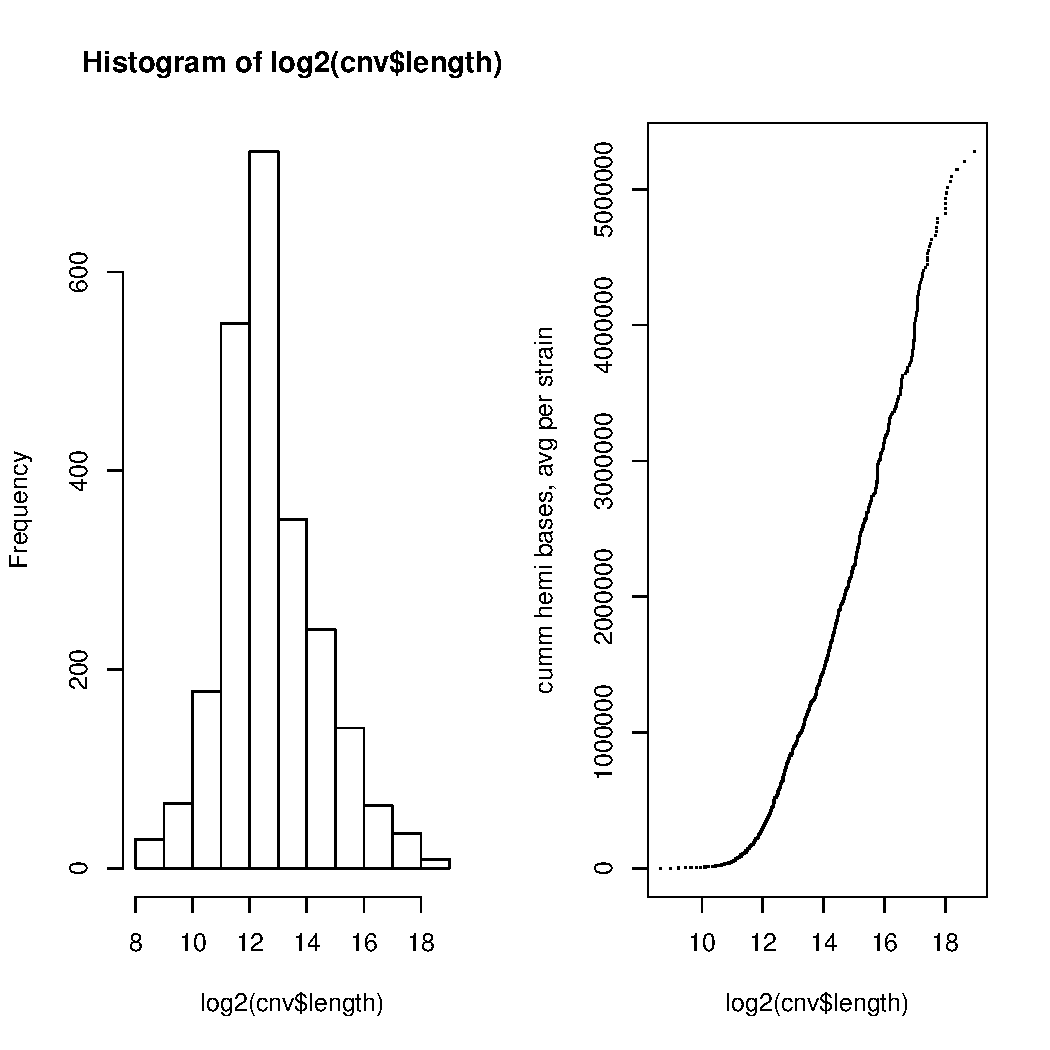
\includegraphics[width=\maxwidth]{figs-knitr/unnamed-chunk-12-1} 

}



\end{knitrout}

\section{Recreating the Time-In-Culture Plot}

Per Chris' 10/3/2014 email, Michaela made the original TIC graph based on filtered = False, $0.3 < \verb|cov_ratio| < 0.8$, only on chromosomes. (gawk 1-liner broken over 3 for print purposes.)
{\small
\begin{verbatim}
gawk 'NR > 1 && $7 == "CNVnator" && $6 == "False" && $8 >.3 && $8 < .7 && \
  substr($2,1,3) == "Chr" {x[$1] += $5} END \
  {for (strain in x) {print strain " " x[strain]}}' cnv.txt

tp1012 1619100
tp1013 1374400
tp1014 495100
tp1015 935600
tp1007 1595600
tp1335 1428700
\end{verbatim}
}%small

Can we reproduce that? For each strain, count number and total length of non-filtered regions on Chr's with coverage ratio in 10 equal bins from 0.0 to 1.0.

\begin{knitrout}\footnotesize
\definecolor{shadecolor}{rgb}{0.969, 0.969, 0.969}\color{fgcolor}\begin{kframe}
\begin{alltt}
\hlkwd{any}\hlstd{(cnv}\hlopt{$}\hlstd{cov_ratio}\hlopt{==}\hlnum{1.0}\hlstd{)} \hlcom{## FALSE}
\end{alltt}
\begin{verbatim}
# [1] FALSE
\end{verbatim}
\begin{alltt}
\hlkwd{any}\hlstd{(cnv}\hlopt{$}\hlstd{cov_ratio}\hlopt{==}\hlnum{0.9}\hlstd{)} \hlcom{## FALSE}
\end{alltt}
\begin{verbatim}
# [1] FALSE
\end{verbatim}
\begin{alltt}
\hlkwd{any}\hlstd{(cnv}\hlopt{$}\hlstd{cov_ratio}\hlopt{==}\hlnum{0.8}\hlstd{)} \hlcom{## FALSE}
\end{alltt}
\begin{verbatim}
# [1] FALSE
\end{verbatim}
\begin{alltt}
\hlkwd{any}\hlstd{(cnv}\hlopt{$}\hlstd{cov_ratio}\hlopt{==}\hlnum{0.7}\hlstd{)} \hlcom{## FALSE}
\end{alltt}
\begin{verbatim}
# [1] FALSE
\end{verbatim}
\begin{alltt}
\hlkwd{any}\hlstd{(cnv}\hlopt{$}\hlstd{cov_ratio}\hlopt{==}\hlnum{0.3}\hlstd{)} \hlcom{## FALSE}
\end{alltt}
\begin{verbatim}
# [1] FALSE
\end{verbatim}
\begin{alltt}
\hlkwd{sum}\hlstd{(cnv}\hlopt{$}\hlstd{cov_ratio}\hlopt{==}\hlnum{0.0}\hlstd{)} \hlcom{## 26, but only 1 not filtered, chromosomal:}
\end{alltt}
\begin{verbatim}
# [1] 26
\end{verbatim}
\begin{alltt}
\hlstd{cnv[cnv}\hlopt{$}\hlstd{cov_ratio}\hlopt{==}\hlnum{0.0} \hlopt{& !}\hlstd{cnv}\hlopt{$}\hlstd{filtered} \hlopt{&} \hlkwd{substr}\hlstd{(cnv}\hlopt{$}\hlstd{chr,}\hlnum{1}\hlstd{,}\hlnum{3}\hlstd{)}\hlopt{==}\hlstr{'Chr'}\hlstd{,]}
\end{alltt}
\begin{verbatim}
#     strain    chr start   end length filtered     type cov_ratio  dup_frac
# 248 tp1012 Chr11a 42601 44200   1600    FALSE CNVnator         0 0.0124481
\end{verbatim}
\begin{alltt}
\hlcom{# how many satisfy filtering criteria??}
\hlkwd{sum}\hlstd{(}\hlopt{!}\hlstd{cnv}\hlopt{$}\hlstd{filtered)} \hlcom{## [1] 2020}
\end{alltt}
\begin{verbatim}
# [1] 2020
\end{verbatim}
\begin{alltt}
\hlkwd{sum}\hlstd{(}\hlkwd{substr}\hlstd{(}\hlkwd{as.character}\hlstd{(cnv}\hlopt{$}\hlstd{chr),}\hlnum{1}\hlstd{,}\hlnum{3}\hlstd{)} \hlopt{==} \hlstr{'Chr'}\hlstd{)}  \hlcom{## [1] 1956}
\end{alltt}
\begin{verbatim}
# [1] 1956
\end{verbatim}
\begin{alltt}
\hlkwd{sum}\hlstd{(cnv}\hlopt{$}\hlstd{cov_ratio} \hlopt{<=} \hlnum{1.0}\hlstd{)}  \hlcom{## [1] 796}
\end{alltt}
\begin{verbatim}
# [1] 796
\end{verbatim}
\begin{alltt}
\hlkwd{sum}\hlstd{(}\hlopt{!}\hlstd{cnv}\hlopt{$}\hlstd{filtered} \hlopt{&} \hlkwd{substr}\hlstd{(}\hlkwd{as.character}\hlstd{(cnv}\hlopt{$}\hlstd{chr),}\hlnum{1}\hlstd{,}\hlnum{3}\hlstd{)} \hlopt{==} \hlstr{'Chr'} \hlopt{&} \hlstd{cnv}\hlopt{$}\hlstd{cov_ratio} \hlopt{<=} \hlnum{1.0}\hlstd{)} \hlcom{## [1] 412}
\end{alltt}
\begin{verbatim}
# [1] 412
\end{verbatim}
\begin{alltt}
\hlstd{pick} \hlkwb{<-} \hlopt{!}\hlstd{cnv}\hlopt{$}\hlstd{filtered} \hlopt{&} \hlkwd{substr}\hlstd{(}\hlkwd{as.character}\hlstd{(cnv}\hlopt{$}\hlstd{chr),}\hlnum{1}\hlstd{,}\hlnum{3}\hlstd{)} \hlopt{==} \hlstr{'Chr'} \hlopt{&} \hlstd{cnv}\hlopt{$}\hlstd{cov_ratio} \hlopt{<=} \hlnum{1.0}
\hlstd{cov.intervals} \hlkwb{<-}\hlkwd{paste}\hlstd{(}\hlstr{'('}\hlstd{,} \hlkwd{seq}\hlstd{(}\hlnum{0.0}\hlstd{,} \hlnum{0.9}\hlstd{,} \hlnum{0.1}\hlstd{),} \hlstr{','}\hlstd{,} \hlkwd{seq}\hlstd{(}\hlnum{0.1}\hlstd{,} \hlnum{1.0}\hlstd{,} \hlnum{0.1}\hlstd{),} \hlstr{']'}\hlstd{,} \hlkwc{sep}\hlstd{=}\hlstr{''}\hlstd{)}
\hlstd{low.length} \hlkwb{<-} \hlkwd{matrix}\hlstd{(}\hlnum{0}\hlstd{,}\hlnum{10}\hlstd{,}\hlnum{7}\hlstd{,}\hlkwc{dimnames}\hlstd{=}\hlkwd{list}\hlstd{(cov.intervals, strain.names))}
\hlstd{low.counts} \hlkwb{<-} \hlkwd{matrix}\hlstd{(}\hlnum{0}\hlstd{,}\hlnum{10}\hlstd{,}\hlnum{7}\hlstd{,}\hlkwc{dimnames}\hlstd{=}\hlkwd{list}\hlstd{(cov.intervals, strain.names))}
\hlcom{#pack <- logical(nrow(cnv))}
\hlkwa{for}\hlstd{(i} \hlkwa{in} \hlnum{1}\hlopt{:}\hlkwd{nrow}\hlstd{(cnv))\{}
  \hlkwa{if}\hlstd{(}\hlopt{!}\hlstd{cnv}\hlopt{$}\hlstd{filtered[i]} \hlopt{&&} \hlkwd{substr}\hlstd{(}\hlkwd{as.character}\hlstd{(cnv}\hlopt{$}\hlstd{chr[i]),}\hlnum{1}\hlstd{,}\hlnum{3}\hlstd{)} \hlopt{==} \hlstr{'Chr'} \hlopt{&&} \hlstd{cnv}\hlopt{$}\hlstd{cov_ratio[i]} \hlopt{<=} \hlnum{1.0}\hlstd{)\{}
    \hlcom{#pack[i] <- T}
    \hlstd{rat} \hlkwb{<-} \hlkwd{ceiling}\hlstd{(cnv}\hlopt{$}\hlstd{cov_ratio[i]} \hlopt{*} \hlnum{10}\hlstd{)}
    \hlstd{st}  \hlkwb{<-} \hlkwd{as.character}\hlstd{(cnv}\hlopt{$}\hlstd{strain[i])}
    \hlstd{low.counts[rat,st]} \hlkwb{<-} \hlstd{low.counts[rat,st]} \hlopt{+} \hlnum{1}
    \hlstd{low.length[rat,st]} \hlkwb{<-} \hlstd{low.length[rat,st]} \hlopt{+} \hlstd{cnv}\hlopt{$}\hlstd{length[i]}
  \hlstd{\}}
\hlstd{\}}
\hlcom{# pick == pack & 412 entries, but one of them has zero ratio, so excluded from counts}
\hlstd{low.counts.37} \hlkwb{<-} \hlkwd{colSums}\hlstd{(low.counts[}\hlnum{4}\hlopt{:}\hlnum{7}\hlstd{,]) ; low.counts.37}
\end{alltt}
\begin{verbatim}
# tp1007 tp1012 tp1013 tp1014 tp1015     IT tp1335 
#     34     47     50     11     27     68     34
\end{verbatim}
\begin{alltt}
\hlstd{low.length.37} \hlkwb{<-} \hlkwd{colSums}\hlstd{(low.length[}\hlnum{4}\hlopt{:}\hlnum{7}\hlstd{,]) ; low.length.37}
\end{alltt}
\begin{verbatim}
#  tp1007  tp1012  tp1013  tp1014  tp1015      IT  tp1335 
# 1595600 1619100 1374400  495100  935600  269900 1428700
\end{verbatim}
\begin{alltt}
\hlcom{# lengths match Chris' email (excluding IT, which he didn't report)}
\hlcom{# tp1007  tp1012  tp1013  tp1014  tp1015      IT  tp1335 }
\hlcom{#1595600 1619100 1374400  495100  935600  269900 1428700 }
\hlstd{low.counts.38} \hlkwb{<-} \hlkwd{colSums}\hlstd{(low.counts[}\hlnum{4}\hlopt{:}\hlnum{8}\hlstd{,]) ; low.counts.38}
\end{alltt}
\begin{verbatim}
# tp1007 tp1012 tp1013 tp1014 tp1015     IT tp1335 
#     40     60     53     24     34     77     38
\end{verbatim}
\begin{alltt}
\hlstd{low.length.38} \hlkwb{<-} \hlkwd{colSums}\hlstd{(low.length[}\hlnum{4}\hlopt{:}\hlnum{8}\hlstd{,]) ; low.length.38}
\end{alltt}
\begin{verbatim}
#  tp1007  tp1012  tp1013  tp1014  tp1015      IT  tp1335 
# 1672500 1781500 1399400 1313700  988400  336500 1453000
\end{verbatim}
\begin{alltt}
\hlstd{low.length.all} \hlkwb{<-} \hlkwd{colSums}\hlstd{(low.length) ; low.length.all}
\end{alltt}
\begin{verbatim}
#  tp1007  tp1012  tp1013  tp1014  tp1015      IT  tp1335 
# 1708500 1813000 1432300 1342200 1007100  426600 1468300
\end{verbatim}
\begin{alltt}
\hlkwd{cbind}\hlstd{(low.length, low.counts)}
\end{alltt}
\begin{verbatim}
#            tp1007  tp1012  tp1013 tp1014 tp1015     IT  tp1335 tp1007 tp1012 tp1013 tp1014 tp1015
# (0,0.1]     28300   26500   11800  28500  14700  33000   14800      4      3      1      4      3
# (0.1,0.2]    5400    3500    6400      0   2800  26600     500      7      4      7      0      4
# (0.2,0.3]    2300    1500   14700      0   1200  30500       0      3      2      3      0      1
# (0.3,0.4]    3300    3200   39100      0  20200  29500     500      1      1     12      0      4
# (0.4,0.5]    5500    8800   36800      0   1800  57500    2900      2      1      9      0      1
# (0.5,0.6]  217500  451100  241800      0 405700 131900 1053400      8     16     11      0     10
# (0.6,0.7] 1369300 1156000 1056700 495100 507900  51000  371900     23     29     18     11     12
# (0.7,0.8]   76900  162400   25000 818600  52800  66600   24300      6     13      3     13      7
# (0.8,0.9]       0       0       0      0      0      0       0      0      0      0      0      0
# (0.9,1]         0       0       0      0      0      0       0      0      0      0      0      0
#           IT tp1335
# (0,0.1]    3      3
# (0.1,0.2] 14      1
# (0.2,0.3] 18      0
# (0.3,0.4] 13      1
# (0.4,0.5] 23      3
# (0.5,0.6] 22     17
# (0.6,0.7] 10     13
# (0.7,0.8]  9      4
# (0.8,0.9]  0      0
# (0.9,1]    0      0
\end{verbatim}
\end{kframe}
\end{knitrout}

Nothing was called between 0.8 and 1.0, presumably CNVnator parameters.  Total in the range between 0.3 and 0.7 matches the numbers in Chris' email.  Total in all ranges matches, too, except for 1012, which has one region of ratio zero, that wasn't counted above (my first bin is (0.0, 0.1]).  Below we plot total versus date placed in culture.  The 5 lines are totals in the (.3, .4], (.3,.5], ..., (.3,.8] windows, just to see how each bin contributes to the total.  The clear message, as is also obvious from the length table printed above, is that the .5 to .8 range is where most of the action is.  

\begin{knitrout}\footnotesize
\definecolor{shadecolor}{rgb}{0.969, 0.969, 0.969}\color{fgcolor}\begin{kframe}
\begin{alltt}
\hlstd{dates} \hlkwb{<-} \hlkwd{unlist}\hlstd{(}\hlkwd{lapply}\hlstd{(}\hlnum{1}\hlopt{:}\hlnum{7}\hlstd{,}\hlkwa{function}\hlstd{(}\hlkwc{st}\hlstd{)\{}\hlkwd{as.integer}\hlstd{(}\hlkwd{st.loc}\hlstd{(st,}\hlkwc{id}\hlstd{=F,}\hlkwc{loc}\hlstd{=F,}\hlkwc{date}\hlstd{=T))\}))}
\hlstd{perm} \hlkwb{<-} \hlkwd{order}\hlstd{(dates)}
\hlkwd{plot}\hlstd{(}\hlnum{0}\hlstd{,}\hlnum{0}\hlstd{,}\hlkwc{type}\hlstd{=}\hlstr{'n'}\hlstd{,} \hlkwc{xlim}\hlstd{=}\hlkwd{range}\hlstd{(dates),} \hlkwc{ylim}\hlstd{=}\hlkwd{c}\hlstd{(}\hlnum{0}\hlstd{,}\hlnum{2e6}\hlstd{),} \hlkwc{xlab}\hlstd{=}\hlstr{'Isolation Date'}\hlstd{,} \hlkwc{ylab}\hlstd{=}\hlstr{'Hemizygous Bases'}\hlstd{)}
\hlkwd{lines}\hlstd{(dates[perm], low.length[}\hlnum{4}\hlstd{,perm],}\hlkwc{type}\hlstd{=}\hlstr{'b'}\hlstd{)}
\hlkwa{for}\hlstd{(i} \hlkwa{in} \hlnum{5}\hlopt{:}\hlnum{8}\hlstd{)\{}
  \hlkwd{lines}\hlstd{(dates[perm],} \hlkwd{colSums}\hlstd{(low.length[}\hlnum{4}\hlopt{:}\hlstd{i,perm]),}\hlkwc{type}\hlstd{=}\hlstr{'b'}\hlstd{)}
\hlstd{\}}
\hlstd{ids} \hlkwb{<-} \hlkwd{unlist}\hlstd{(}\hlkwd{lapply}\hlstd{(}\hlnum{1}\hlopt{:}\hlnum{7}\hlstd{,}\hlkwa{function}\hlstd{(}\hlkwc{st}\hlstd{)\{}\hlkwd{st.loc}\hlstd{(st,}\hlkwc{id}\hlstd{=T,}\hlkwc{loc}\hlstd{=F,}\hlkwc{date}\hlstd{=F)\}))}
\hlkwd{text}\hlstd{(dates, low.length.38,} \hlkwc{labels}\hlstd{=ids,}\hlkwc{cex}\hlstd{=}\hlnum{.6}\hlstd{,}\hlkwc{pos}\hlstd{=}\hlnum{3}\hlstd{)}
\hlkwd{points}\hlstd{(dates,low.length.all,}\hlkwc{pch}\hlstd{=}\hlstr{'x'}\hlstd{)}  \hlcom{# showing "all" changes little}
\end{alltt}
\end{kframe}

{\centering 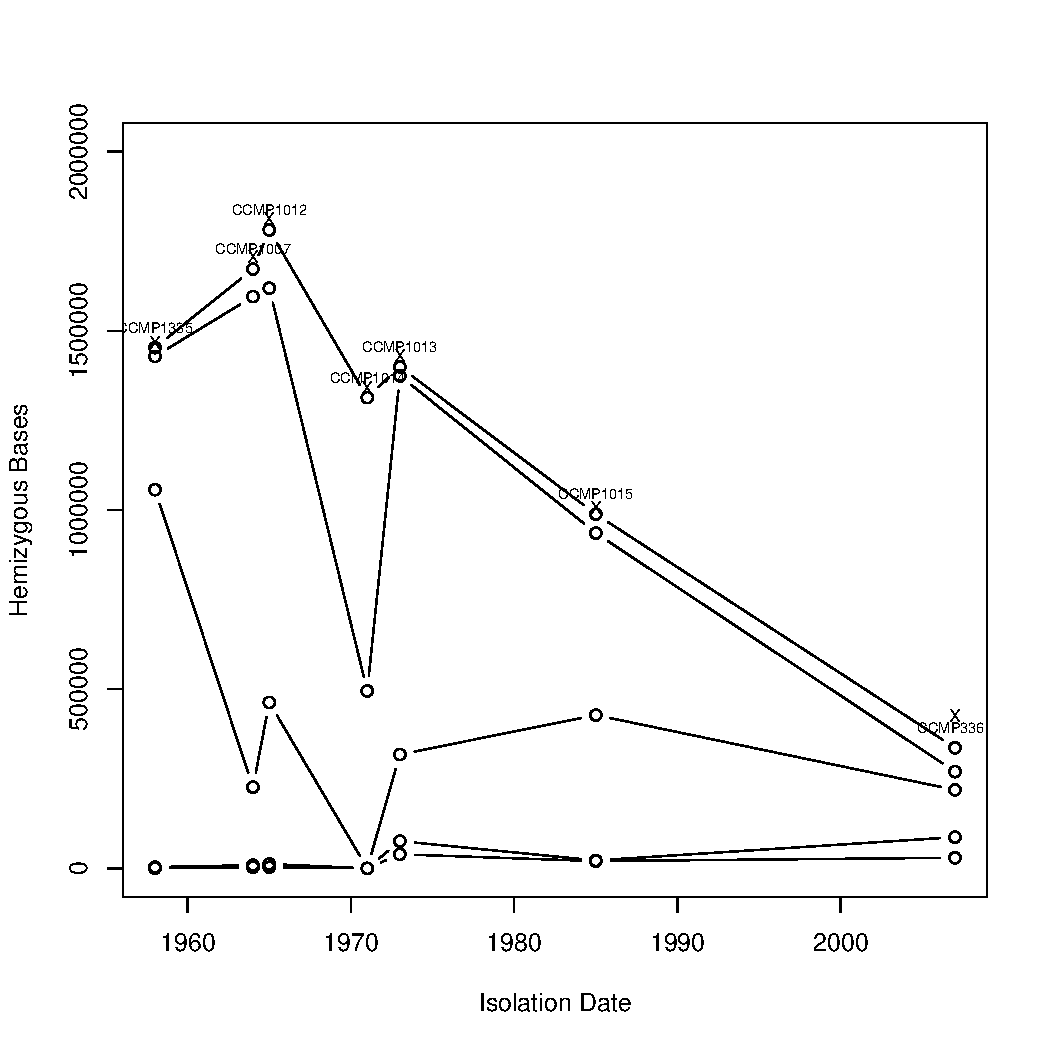
\includegraphics[width=\maxwidth]{figs-knitr/unnamed-chunk-14-1} 

}



\end{knitrout}

The graph Michaela made is most similar to the last (highest) of these, but her Y scale is a bit larger, perhaps due to inclusion of ``non-Chr'' and/or ``filtered'' calls.  I like the above graph better, it seems a bit more conservative, while still showing the interesting trend.

For the paper supplement, I'd just show the .3--.8 points, plus a trend line.

\begin{knitrout}\footnotesize
\definecolor{shadecolor}{rgb}{0.969, 0.969, 0.969}\color{fgcolor}\begin{kframe}
\begin{alltt}
\hlkwd{plot}\hlstd{(dates, low.length.38}\hlopt{/}\hlnum{1000}\hlstd{,}\hlkwc{type}\hlstd{=}\hlstr{'p'}\hlstd{,} \hlkwc{xlim}\hlstd{=}\hlkwd{range}\hlstd{(dates)}\hlopt{+}\hlkwd{c}\hlstd{(}\hlopt{-}\hlnum{2}\hlstd{,}\hlnum{2}\hlstd{),} \hlkwc{ylim}\hlstd{=}\hlkwd{c}\hlstd{(}\hlnum{0}\hlstd{,}\hlnum{2e6}\hlopt{/}\hlnum{1000}\hlstd{),}
     \hlkwc{xlab}\hlstd{=}\hlstr{'Isolation Date'}\hlstd{,} \hlkwc{ylab}\hlstd{=}\hlstr{'Hemizygous Kilobases'}\hlstd{)}
\hlkwd{text}\hlstd{(dates, low.length.38}\hlopt{/}\hlnum{1000}\hlstd{,} \hlkwc{labels}\hlstd{=ids,}\hlkwc{cex}\hlstd{=}\hlnum{.6}\hlstd{,}\hlkwc{pos}\hlstd{=}\hlnum{3}\hlstd{)}
\hlkwd{abline}\hlstd{(}\hlkwd{lm}\hlstd{(low.length.38}\hlopt{/}\hlnum{1000} \hlopt{~} \hlstd{dates)}\hlopt{$}\hlstd{coefficients)}
\hlkwd{text}\hlstd{(}\hlnum{1990}\hlstd{,}\hlnum{1.5e6}\hlopt{/}\hlnum{1000}\hlstd{,} \hlkwd{paste}\hlstd{(}\hlstr{'rho ='}\hlstd{,}\hlkwd{format}\hlstd{(}\hlkwd{cor}\hlstd{(low.length.38 , dates),}\hlkwc{digits}\hlstd{=}\hlnum{2}\hlstd{)))}
\end{alltt}
\end{kframe}

{\centering 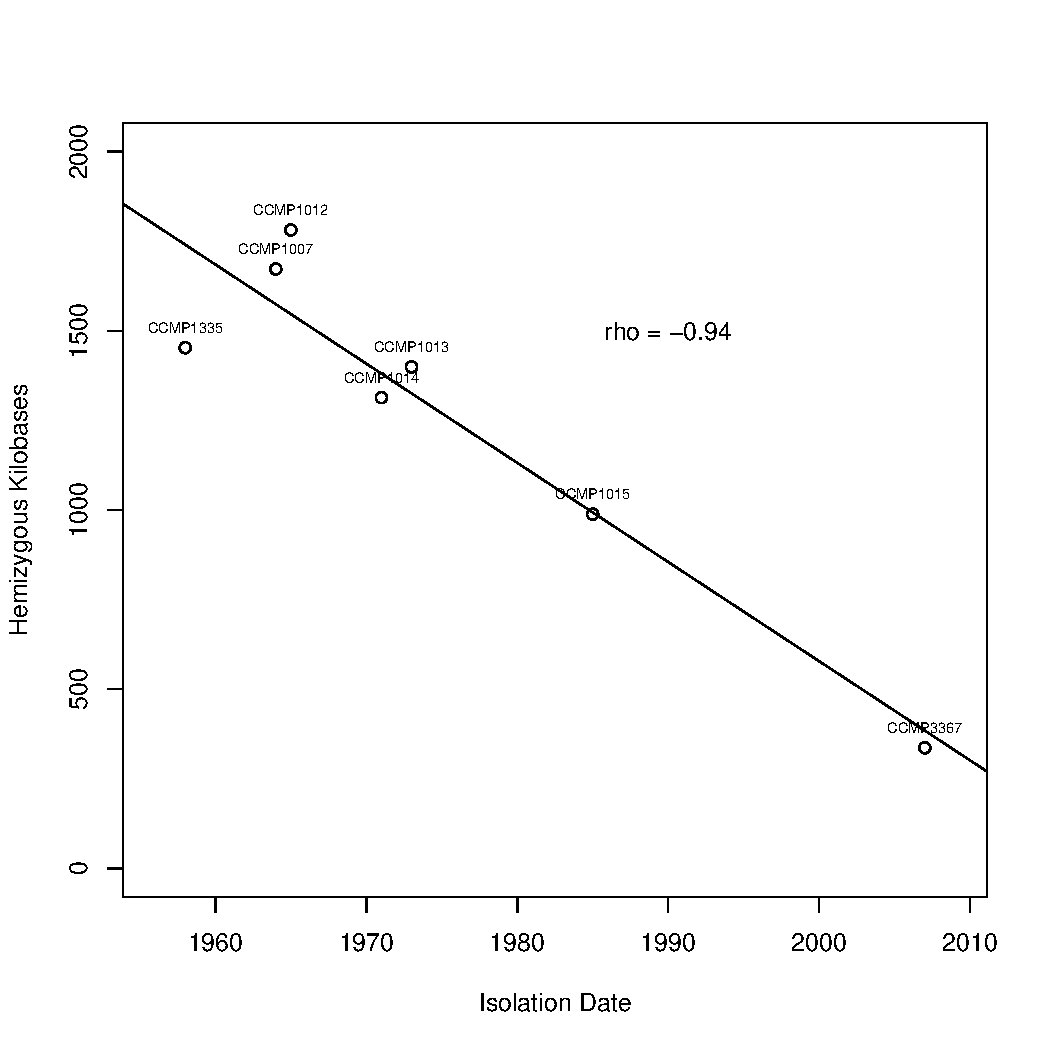
\includegraphics[width=\maxwidth]{figs-knitr/old-hemizygosity-supp-fig-1} 

}



\end{knitrout}

Make the same plot for any coverage slice, optionally with fancy legend:

\begin{knitrout}\footnotesize
\definecolor{shadecolor}{rgb}{0.969, 0.969, 0.969}\color{fgcolor}\begin{kframe}
\begin{alltt}
\hlstd{tic} \hlkwb{<-} \hlkwa{function}\hlstd{(}\hlkwc{lo}\hlstd{=}\hlnum{0.3}\hlstd{,} \hlkwc{hi}\hlstd{=}\hlnum{0.8}\hlstd{,}                           \hlcom{# coverage thresholds}
                \hlkwc{cnv.tbl}\hlstd{=cnv,} \hlkwc{thedates}\hlstd{=dates,} \hlkwc{theids}\hlstd{=ids,}  \hlcom{# stuff computed above}
                \hlkwc{theylim}\hlstd{=}\hlkwa{NULL}\hlstd{,}                             \hlcom{# y axis limits}
                \hlkwc{fancy}\hlstd{=}\hlnum{FALSE}\hlstd{,} \hlkwc{legcex}\hlstd{=}\hlnum{0.7}                   \hlcom{# fancy legend}
                \hlstd{)\{}
  \hlstd{opar} \hlkwb{<-} \hlkwd{par}\hlstd{(}\hlkwc{no.readonly}\hlstd{=}\hlnum{TRUE}\hlstd{);} \hlkwd{on.exit}\hlstd{(}\hlkwd{par}\hlstd{(opar))}
  \hlstd{pick} \hlkwb{<-} \hlopt{!}\hlstd{cnv.tbl}\hlopt{$}\hlstd{filtered} \hlopt{&} \hlkwd{substr}\hlstd{(}\hlkwd{as.character}\hlstd{(cnv.tbl}\hlopt{$}\hlstd{chr),}\hlnum{1}\hlstd{,}\hlnum{3}\hlstd{)} \hlopt{==} \hlstr{'Chr'} \hlopt{&}
          \hlstd{lo} \hlopt{<=} \hlstd{cnv.tbl}\hlopt{$}\hlstd{cov_ratio} \hlopt{&} \hlstd{cnv.tbl}\hlopt{$}\hlstd{cov_ratio} \hlopt{<=} \hlstd{hi}
  \hlstd{lengths} \hlkwb{<-} \hlkwd{matrix}\hlstd{(}\hlnum{NA}\hlstd{,}\hlnum{7}\hlstd{,}\hlnum{1}\hlstd{,}\hlkwc{dimnames}\hlstd{=}\hlkwd{list}\hlstd{(}\hlkwd{rep}\hlstd{(}\hlstr{''}\hlstd{,}\hlnum{7}\hlstd{)))}
  \hlkwa{for}\hlstd{(st} \hlkwa{in} \hlnum{1}\hlopt{:}\hlkwd{nlevels}\hlstd{(cnv.tbl}\hlopt{$}\hlstd{strain))\{}
    \hlstd{st.fact} \hlkwb{<-} \hlkwd{levels}\hlstd{(cnv.tbl}\hlopt{$}\hlstd{strain)[st]}
    \hlkwd{rownames}\hlstd{(lengths)[st]} \hlkwb{<-} \hlstd{st.fact}
    \hlstd{lengths[st]} \hlkwb{<-} \hlkwd{sum}\hlstd{(cnv.tbl}\hlopt{$}\hlstd{length[pick} \hlopt{&} \hlstd{cnv.tbl}\hlopt{$}\hlstd{strain}\hlopt{==}\hlstd{st.fact])}
  \hlstd{\}}
  \hlstd{lengths} \hlkwb{<-} \hlstd{lengths[}\hlkwd{c}\hlstd{(}\hlnum{2}\hlopt{:}\hlnum{6}\hlstd{,}\hlnum{1}\hlstd{,}\hlnum{7}\hlstd{),]} \hlcom{# reorder}
  \hlkwa{if}\hlstd{(}\hlkwd{is.null}\hlstd{(theylim))\{theylim} \hlkwb{<-} \hlkwd{range}\hlstd{(lengths)}\hlopt{/}\hlnum{1000}\hlstd{\}}
  \hlkwd{plot}\hlstd{(thedates, lengths}\hlopt{/}\hlnum{1000}\hlstd{,} \hlkwc{type}\hlstd{=}\hlstr{'p'}\hlstd{,}
       \hlkwc{xlim}\hlstd{=}\hlkwd{range}\hlstd{(thedates)}\hlopt{+}\hlkwd{c}\hlstd{(}\hlopt{-}\hlnum{2}\hlstd{,}\hlnum{2}\hlstd{),}
       \hlkwc{ylim}\hlstd{=theylim,}
       \hlkwc{xlab}\hlstd{=}\hlstr{'Isolation Date (Year)'}\hlstd{,}
       \hlkwc{ylab}\hlstd{=}\hlkwd{ifelse}\hlstd{(fancy,} \hlstr{'Estimated Hemizygous Deletion (Kilobases)'}\hlstd{,}
                   \hlkwd{paste}\hlstd{(}\hlstr{'Kbases w/ cov_ratio in ['}\hlstd{, lo,} \hlstr{','}\hlstd{, hi,} \hlstr{']'}\hlstd{,}\hlkwc{sep}\hlstd{=}\hlstr{''}\hlstd{)}
       \hlstd{),}
       \hlkwc{pch}\hlstd{=}\hlkwd{ifelse}\hlstd{(fancy,}\hlnum{19}\hlstd{,}\hlnum{1}\hlstd{)}
  \hlstd{)}
  \hlkwa{if}\hlstd{(fancy)\{}
    \hlstd{theids} \hlkwb{<-} \hlkwd{st.locs}\hlstd{(}\hlnum{1}\hlopt{:}\hlnum{7}\hlstd{,}\hlkwc{id}\hlstd{=F,}\hlkwc{loc}\hlstd{=F,}\hlkwc{locabbrv}\hlstd{=T,}\hlkwc{date}\hlstd{=F)}
  \hlstd{\}}
  \hlkwd{text}\hlstd{(thedates, lengths}\hlopt{/}\hlnum{1000}\hlstd{,} \hlkwc{cex}\hlstd{=legcex,} \hlkwc{pos}\hlstd{=}\hlkwd{ifelse}\hlstd{(fancy,} \hlnum{2}\hlstd{,} \hlnum{3}\hlstd{),} \hlkwc{labels}\hlstd{=theids)}
  \hlkwd{abline}\hlstd{(}\hlkwd{lm}\hlstd{(lengths}\hlopt{/}\hlnum{1000} \hlopt{~} \hlstd{thedates)}\hlopt{$}\hlstd{coefficients)}
  \hlkwd{legend}\hlstd{(}\hlkwd{ifelse}\hlstd{(fancy,} \hlstr{'bottomleft'}\hlstd{,} \hlstr{'topright'}\hlstd{),}
         \hlkwc{legend}\hlstd{=}\hlkwd{paste}\hlstd{(}\hlstr{'rho ='}\hlstd{,} \hlkwd{format}\hlstd{(}\hlkwd{cor}\hlstd{(lengths}\hlopt{/}\hlnum{1000} \hlstd{, thedates),}\hlkwc{digits}\hlstd{=}\hlnum{2}\hlstd{)),}
         \hlkwc{bty}\hlstd{=}\hlstr{'n'}\hlstd{,} \hlkwc{cex}\hlstd{=legcex)}
  \hlkwa{if}\hlstd{(fancy)\{}
    \hlstd{thelocs} \hlkwb{<-} \hlkwd{st.locs}\hlstd{(}\hlnum{1}\hlopt{:}\hlnum{7}\hlstd{,}\hlkwc{id}\hlstd{=F,}\hlkwc{loc}\hlstd{=T,}\hlkwc{locabbrv}\hlstd{=F,}\hlkwc{date}\hlstd{=F)}
    \hlstd{thelocdate} \hlkwb{<-} \hlkwd{paste}\hlstd{(} \hlstr{' - '} \hlstd{, thelocs,} \hlstr{' ('}\hlstd{, thedates,} \hlstr{')'}\hlstd{,} \hlkwc{sep}\hlstd{=}\hlstr{''}\hlstd{)}
    \hlcom{# getting legend to align nicely using non-monospaced font is a bit fussy.}
    \hlcom{# Use "text()" to place strain "loc abbrev" (theids) separately from }
    \hlcom{# " - full.loc (dates)" (thelocdate) so that I can control x-position.   }
    \hlcom{# Put legend at upper right.  Several arbitrary constants below (lines marked **)}
    \hlcom{# reflect empirical fiddling to make it look nice: top @ 25Kb below max y, }
    \hlcom{# right edge @ 2009, 1.5x line spacing, rectangle margin}
    \hlstd{widest.locdate} \hlkwb{<-} \hlkwd{max}\hlstd{(}\hlkwd{strwidth}\hlstd{(thelocdate,} \hlkwc{cex}\hlstd{=legcex))} \hlcom{# widest location/date}
    \hlstd{widest.abbrv}   \hlkwb{<-} \hlkwd{max}\hlstd{(}\hlkwd{strwidth}\hlstd{(theids,} \hlkwc{cex}\hlstd{=legcex))}     \hlcom{# widest loc abbreviation}
    \hlstd{height}         \hlkwb{<-} \hlkwd{max}\hlstd{(}\hlkwd{strheight}\hlstd{(thelocdate,} \hlkwc{cex}\hlstd{=legcex))}\hlcom{# text height}
    \hlstd{yby}  \hlkwb{<-} \hlstd{height} \hlopt{*} \hlnum{1.5}                                    \hlcom{# ** line spacing}
  \hlcom{# maxy <- max(lengths)/1000 - 25                          # ** top just below highest point}
    \hlstd{maxy} \hlkwb{<-} \hlstd{theylim[}\hlnum{2}\hlstd{]} \hlopt{-} \hlstd{height} \hlopt{-} \hlnum{25}                        \hlcom{# ** top just below y axis limit}
    \hlstd{ys}   \hlkwb{<-} \hlkwd{seq}\hlstd{(}\hlkwc{from}\hlstd{=maxy,} \hlkwc{by}\hlstd{=}\hlopt{-}\hlstd{yby,} \hlkwc{length.out}\hlstd{=}\hlnum{7}\hlstd{)}           \hlcom{#    y-coords for each line}
    \hlstd{x2}   \hlkwb{<-} \hlnum{2009} \hlopt{-} \hlstd{widest.locdate}                           \hlcom{# ** right edge @ 2009}
    \hlstd{x1}   \hlkwb{<-}   \hlstd{x2} \hlopt{-} \hlstd{widest.abbrv}
    \hlkwd{rect}\hlstd{(x1}\hlopt{-}\hlnum{1.0}\hlstd{, maxy}\hlopt{-}\hlnum{7.2}\hlopt{*}\hlstd{yby,} \hlnum{2009}\hlopt{+}\hlnum{1.0}\hlstd{, maxy}\hlopt{+}\hlnum{1.2}\hlopt{*}\hlstd{yby)}      \hlcom{# ** inflate rectangle slightly}
    \hlkwd{text}\hlstd{(x1, ys,} \hlkwc{cex}\hlstd{=legcex,} \hlkwc{adj}\hlstd{=}\hlnum{0}\hlstd{,} \hlkwc{labels}\hlstd{=theids[}\hlkwd{order}\hlstd{(dates)])}
    \hlkwd{text}\hlstd{(x2, ys,} \hlkwc{cex}\hlstd{=legcex,} \hlkwc{adj}\hlstd{=}\hlnum{0}\hlstd{,} \hlkwc{labels}\hlstd{=thelocdate[}\hlkwd{order}\hlstd{(dates)])}
  \hlstd{\}}
  \hlkwd{return}\hlstd{(lengths)}
\hlstd{\}}
\end{alltt}
\end{kframe}
\end{knitrout}

\begin{knitrout}\footnotesize
\definecolor{shadecolor}{rgb}{0.969, 0.969, 0.969}\color{fgcolor}\begin{kframe}
\begin{alltt}
\hlkwd{tic}\hlstd{()} \hlcom{# debug test: duplicate graph above?}
\end{alltt}
\begin{verbatim}
#  tp1007  tp1012  tp1013  tp1014  tp1015      IT  tp1335 
# 1672500 1781500 1399400 1313700  988400  336500 1453000
\end{verbatim}
\end{kframe}

{\centering 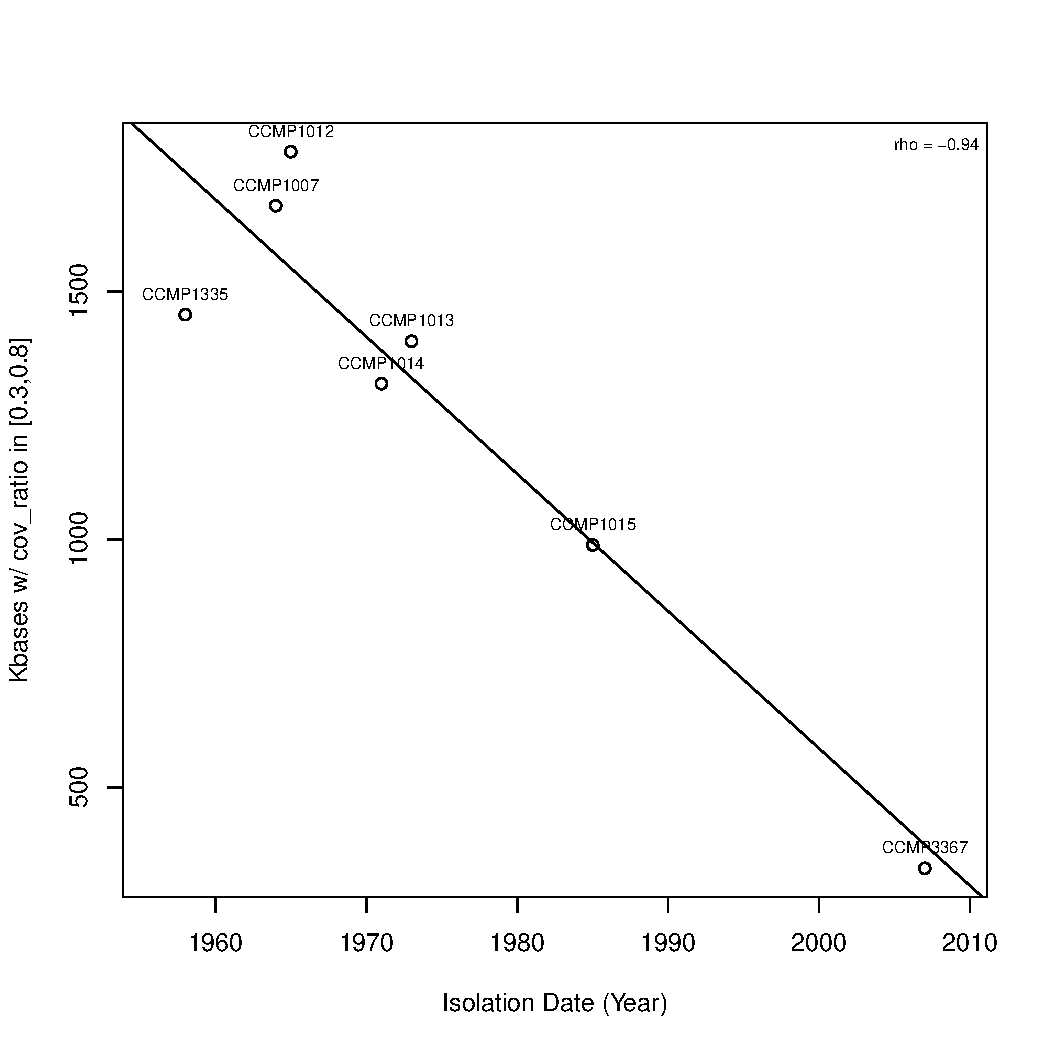
\includegraphics[width=\maxwidth]{figs-knitr/unnamed-chunk-16-1} 

}



\end{knitrout}

\begin{knitrout}\footnotesize
\definecolor{shadecolor}{rgb}{0.969, 0.969, 0.969}\color{fgcolor}\begin{kframe}
\begin{alltt}
\hlstd{fig.S4.path} \hlkwb{<-} \hlkwd{paste}\hlstd{(my.figs.dir,} \hlstr{'FigS4-hemizygosity.pdf'}\hlstd{,} \hlkwc{sep}\hlstd{=}\hlstr{''}\hlstd{)}
\hlkwd{pdf}\hlstd{(fig.S4.path,}\hlkwc{height}\hlstd{=}\hlnum{5}\hlstd{,}\hlkwc{width}\hlstd{=}\hlnum{6}\hlstd{)}
\hlkwd{tic}\hlstd{(}\hlkwc{fancy}\hlstd{=}\hlnum{TRUE}\hlstd{,}\hlkwc{theylim}\hlstd{=}\hlkwd{c}\hlstd{(}\hlnum{0}\hlstd{,}\hlnum{2e6}\hlopt{/}\hlnum{1000}\hlstd{))} \hlcom{# fancy version for paper (Supp Fig S4).}
\end{alltt}
\begin{verbatim}
#  tp1007  tp1012  tp1013  tp1014  tp1015      IT  tp1335 
# 1672500 1781500 1399400 1313700  988400  336500 1453000
\end{verbatim}
\begin{alltt}
\hlkwd{dev.off}\hlstd{()}
\end{alltt}
\begin{verbatim}
# pdf 
#   2
\end{verbatim}
\end{kframe}
\end{knitrout}
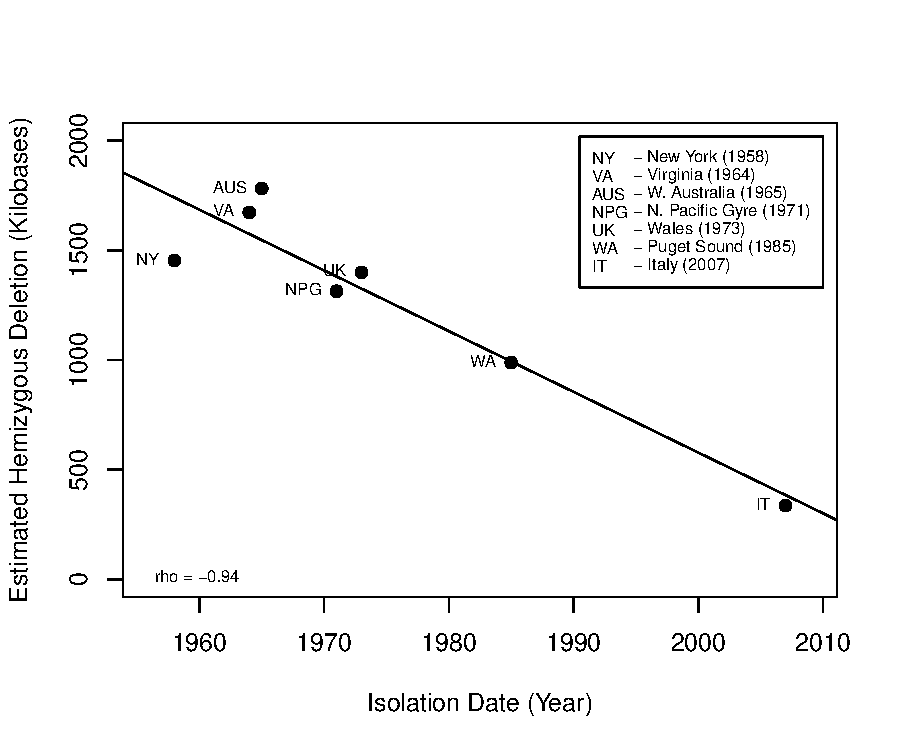
\includegraphics{figs-mine/FigS4-hemizygosity.pdf}

\section{Time-In-Culture for Above-Average Coverages}

\begin{knitrout}\footnotesize
\definecolor{shadecolor}{rgb}{0.969, 0.969, 0.969}\color{fgcolor}\begin{kframe}
\begin{alltt}
\hlkwd{max}\hlstd{(cnv}\hlopt{$}\hlstd{cov_ratio)}
\end{alltt}
\begin{verbatim}
# [1] 11.7308
\end{verbatim}
\end{kframe}
\end{knitrout}

Time-in-culture also correlates with coverage above 1:

\begin{knitrout}\footnotesize
\definecolor{shadecolor}{rgb}{0.969, 0.969, 0.969}\color{fgcolor}\begin{kframe}
\begin{alltt}
\hlkwd{tic}\hlstd{(}\hlnum{1.2}\hlstd{,}\hlnum{1000}\hlstd{)}
\end{alltt}
\begin{verbatim}
#  tp1007  tp1012  tp1013  tp1014  tp1015      IT  tp1335 
# 2101600 3720500 1606400 4372200 2097500 1227700 2823200
\end{verbatim}
\end{kframe}

{\centering 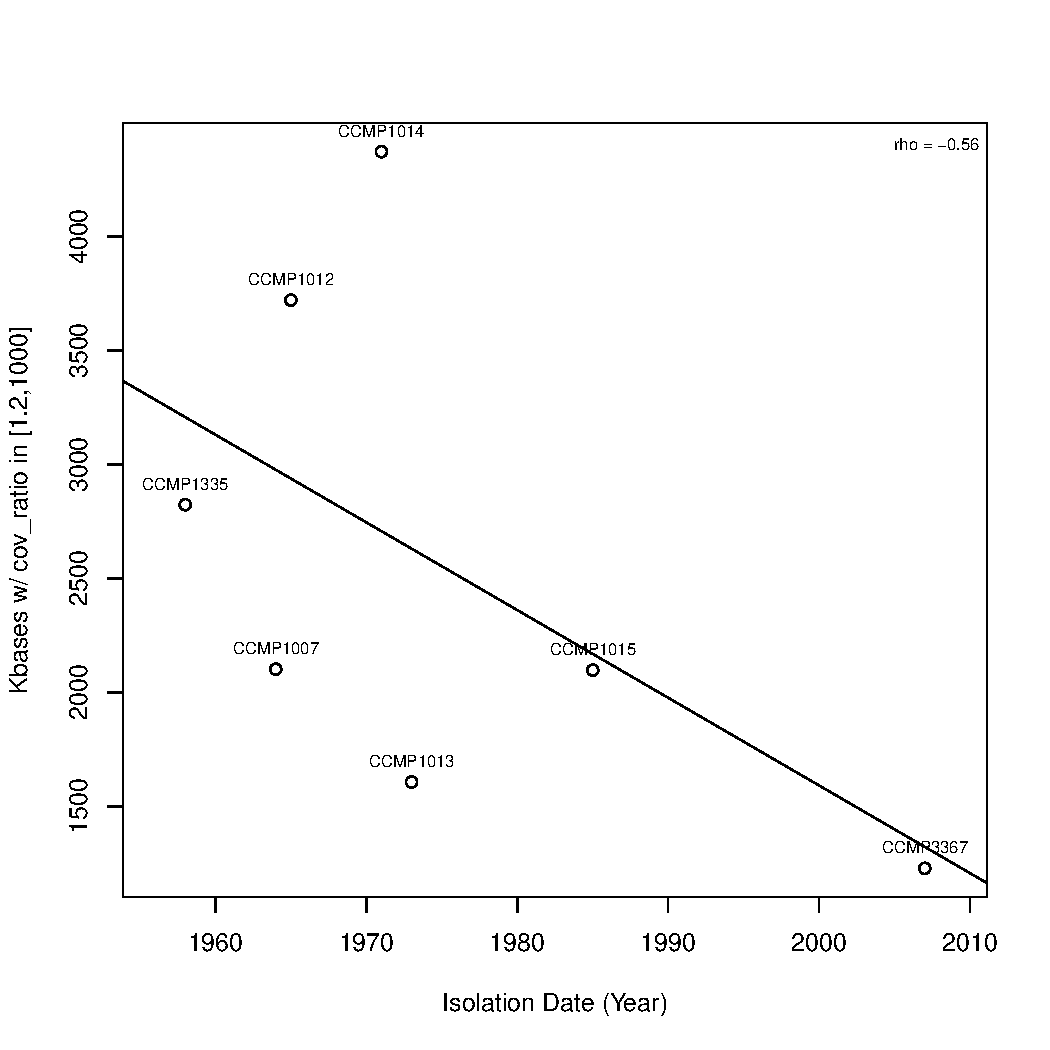
\includegraphics[width=\maxwidth]{figs-knitr/alldups-1} 

}



\end{knitrout}

And with possible trisomies:

\begin{knitrout}\footnotesize
\definecolor{shadecolor}{rgb}{0.969, 0.969, 0.969}\color{fgcolor}\begin{kframe}
\begin{alltt}
\hlkwd{tic}\hlstd{(}\hlnum{1.2}\hlstd{,}\hlnum{1.75}\hlstd{)}
\end{alltt}
\begin{verbatim}
#  tp1007  tp1012  tp1013  tp1014  tp1015      IT  tp1335 
# 1555500 2803600  997300 3457700 1399600  642800 2373400
\end{verbatim}
\end{kframe}

{\centering 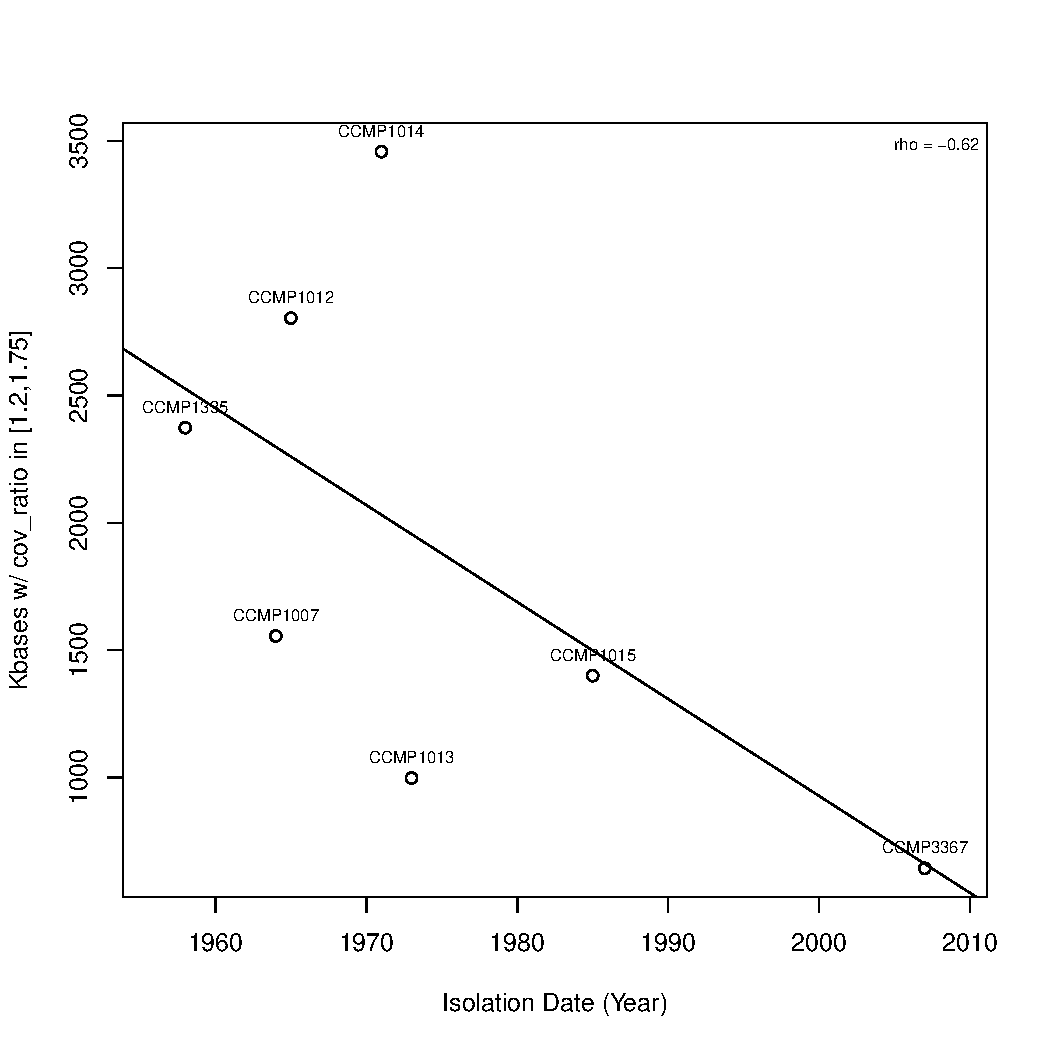
\includegraphics[width=\maxwidth]{figs-knitr/trisomy-1} 

}



\end{knitrout}

But only weakly with duplications:

\begin{knitrout}\footnotesize
\definecolor{shadecolor}{rgb}{0.969, 0.969, 0.969}\color{fgcolor}\begin{kframe}
\begin{alltt}
\hlkwd{tic}\hlstd{(}\hlnum{1.75}\hlstd{,}\hlnum{2.5}\hlstd{)}
\end{alltt}
\begin{verbatim}
# tp1007 tp1012 tp1013 tp1014 tp1015     IT tp1335 
# 403700 734400 454200 777700 569700 352200 269000
\end{verbatim}
\end{kframe}

{\centering 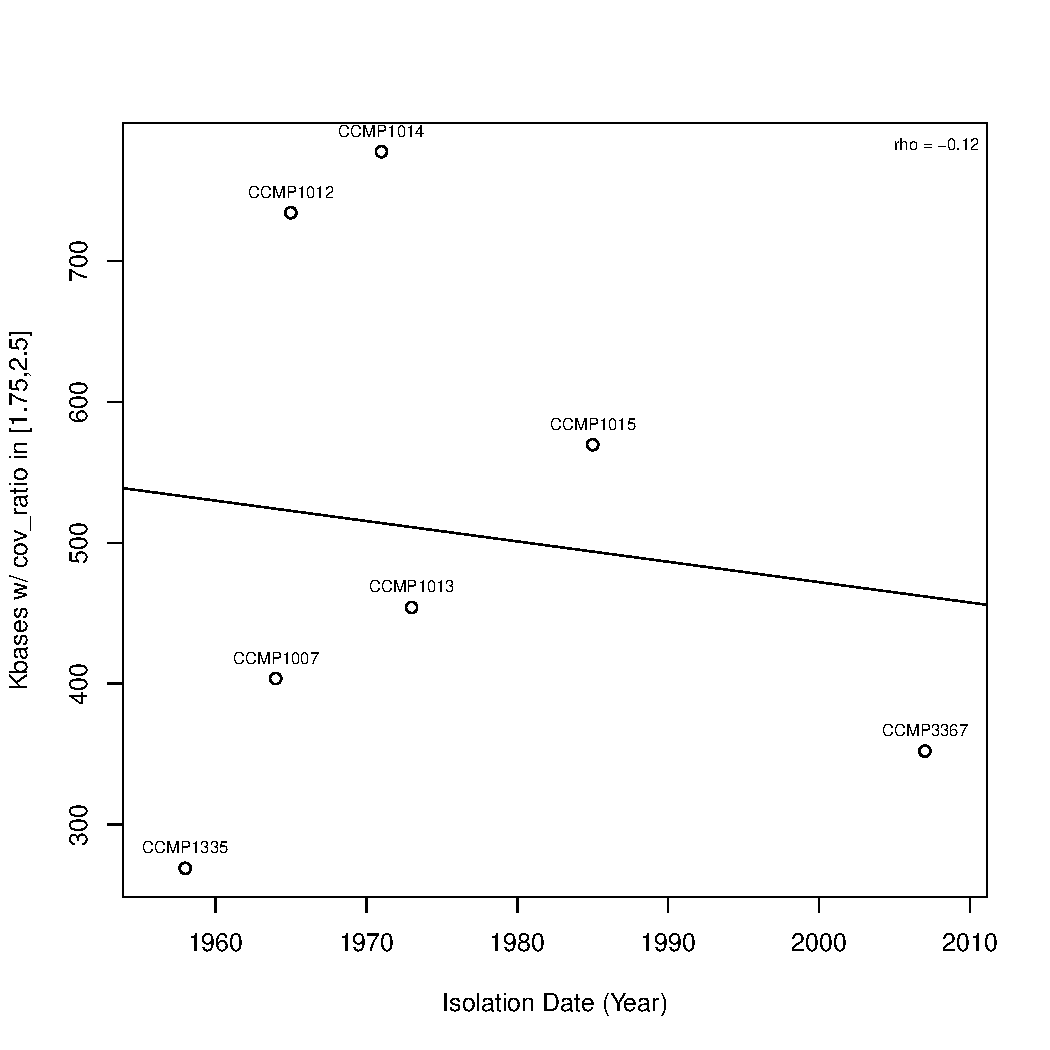
\includegraphics[width=\maxwidth]{figs-knitr/duplication-1} 

}



\end{knitrout}

And not with triplications (or higher), as the totals get smaller/noisier, (although there is a distinct trend if Italy were excluded):

\begin{knitrout}\footnotesize
\definecolor{shadecolor}{rgb}{0.969, 0.969, 0.969}\color{fgcolor}\begin{kframe}
\begin{alltt}
\hlkwd{tic}\hlstd{(}\hlnum{2.5}\hlstd{,}\hlnum{1000}\hlstd{)}
\end{alltt}
\begin{verbatim}
# tp1007 tp1012 tp1013 tp1014 tp1015     IT tp1335 
# 142400 182500 154900 136800 128200 232700 180800
\end{verbatim}
\end{kframe}

{\centering 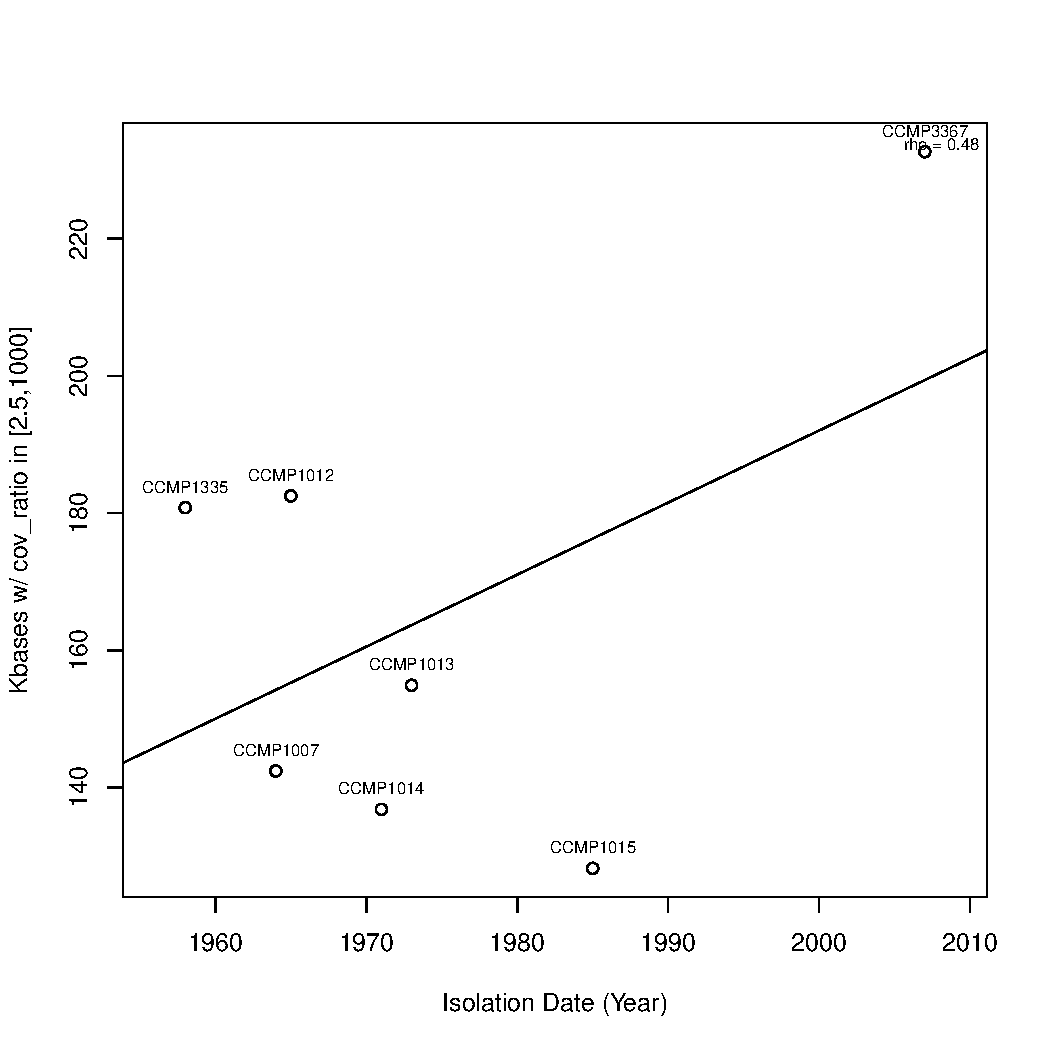
\includegraphics[width=\maxwidth]{figs-knitr/tripleup-1} 

}



\end{knitrout}

\section{Shared/Private Hemizygosity}

A quick eyeball at shared/private
\begin{knitrout}\footnotesize
\definecolor{shadecolor}{rgb}{0.969, 0.969, 0.969}\color{fgcolor}\begin{kframe}
\begin{alltt}
\hlstd{cnvp} \hlkwb{<-} \hlstd{cnv[pick,]}
\hlstd{pi} \hlkwb{<-} \hlkwd{order}\hlstd{(cnvp}\hlopt{$}\hlstd{chr,cnvp}\hlopt{$}\hlstd{start,cnvp}\hlopt{$}\hlstd{length,cnvp}\hlopt{$}\hlstd{strain)}
\hlstd{cnvv} \hlkwb{<-} \hlstd{cnvp[pi,]}
\hlstd{cnvv}
\end{alltt}
\begin{verbatim}
#      strain       chr   start     end length filtered     type   cov_ratio   dup_frac
# 1669     IT      Chr1       1   25200  25200    FALSE CNVnator 0.722468000 0.69837600
# 1    tp1012      Chr1   10601   13500   2900    FALSE CNVnator 0.637380000 0.41187900
# 1366 tp1015      Chr1   10601   14400   3800    FALSE CNVnator 0.706210000 0.45966200
# 508  tp1013      Chr1   16601   25200   8600    FALSE CNVnator 0.636063000 0.68046000
# 1670     IT      Chr1   67901   70700   2800    FALSE CNVnator 0.501551000 0.20650300
# 1671     IT      Chr1   80601   82300   1700    FALSE CNVnator 0.223819000 0.04930390
# 2089 tp1335      Chr1   90501   91800   1300    FALSE CNVnator 0.488495000 0.00997009
# 509  tp1013      Chr1  106601  108600   2000    FALSE CNVnator 0.555534000 0.70172500
# 5    tp1012      Chr1  536501  538600   2100    FALSE CNVnator 0.684861000 0.02109840
# 1676     IT      Chr1  538801  543200   4400    FALSE CNVnator 0.704481000 0.16905200
# 2093 tp1335      Chr1 1222401 1224900   2500    FALSE CNVnator 0.599521000 0.13329200
# 1679     IT      Chr1 1222501 1224400   1900    FALSE CNVnator 0.248841000 0.09708220
# 512  tp1013      Chr1 1222601 1224700   2100    FALSE CNVnator 0.378575000 0.18979700
# 514  tp1013      Chr1 1865001 1865600    600    FALSE CNVnator 0.111020000 0.07031250
# 24   tp1012      Chr1 2464001 2465000   1000    FALSE CNVnator 0.283469000 0.02288490
# 1053 tp1007      Chr1 2464101 2464700    600    FALSE CNVnator 0.199091000 0.03571430
# 1375 tp1015      Chr1 2521201 2525500   4300    FALSE CNVnator 0.546392000 0.02256380
# 1687     IT      Chr1 2545801 2551100   5300    FALSE CNVnator 0.653475000 0.39250500
# 1061 tp1007      Chr1 3042101 3042600    500    FALSE CNVnator 0.188780000 0.52830200
# 31   tp1012      Chr1 3042101 3042600    500    FALSE CNVnator 0.249870000 0.33256000
# 1382 tp1015      Chr1 3042101 3042600    500    FALSE CNVnator 0.187651000 0.37586700
# 2105 tp1335      Chr1 3042101 3042600    500    FALSE CNVnator 0.313598000 0.44981100
# 597  tp1013     Chr10   12301   20100   7800    FALSE CNVnator 0.639332000 0.94901100
# 1826     IT     Chr10   12301   28500  16200    FALSE CNVnator 0.526721000 0.82503700
# 1828     IT     Chr10  103801  104500    700    FALSE CNVnator 0.453978000 0.74776100
# 1831     IT     Chr10  215601  218300   2700    FALSE CNVnator 0.520260000 0.69291000
# 602  tp1013     Chr10  215601  218300   2700    FALSE CNVnator 0.446037000 0.69061400
# 1171 tp1007     Chr10  812601  814700   2100    FALSE CNVnator 0.737270000 0.01840490
# 1835     IT     Chr10  915301  915800    500    FALSE CNVnator 0.262656000 0.03667140
# 608  tp1013    Chr11a       1    5200   5200    FALSE CNVnator 0.498237000 0.66891100
# 1174 tp1007    Chr11a    1001    1800    800    FALSE CNVnator 0.204382000 0.77297300
# 245  tp1012    Chr11a    1001    1800    800    FALSE CNVnator 0.183318000 0.80642000
# 1499 tp1015    Chr11a    1001    1800    800    FALSE CNVnator 0.157815000 0.75340600
# 247  tp1012    Chr11a   12101   20900   8800    FALSE CNVnator 0.417926000 0.85631200
# 1839     IT    Chr11a   12101   21100   9000    FALSE CNVnator 0.434211000 0.84901600
# 1176 tp1007    Chr11a   12101   22300  10200    FALSE CNVnator 0.554710000 0.84839400
# 1501 tp1015    Chr11a   12101   22300  10200    FALSE CNVnator 0.387820000 0.83772200
# 609  tp1013    Chr11a   12101   58500  46400    FALSE CNVnator 0.572295000 0.25616000
# 1840     IT    Chr11a   40901   45300   4400    FALSE CNVnator 0.305445000 0.14415300
# 1178 tp1007    Chr11a   42501   44200   1700    FALSE CNVnator 0.036484300 0.18320600
# 886  tp1014    Chr11a   42501   44300   1800    FALSE CNVnator 0.055698900 0.20939300
# 2203 tp1335    Chr11a   42501   44300   1800    FALSE CNVnator 0.057603600 0.12004700
# 248  tp1012    Chr11a   42601   44200   1600    FALSE CNVnator 0.000000000 0.01244810
# 1502 tp1015    Chr11a   42601   44300   1700    FALSE CNVnator 0.050497400 0.02290080
# 1841     IT    Chr11a   50501   58500   8000    FALSE CNVnator 0.329241000 0.64361100
# 610  tp1013    Chr11a   65801  253100 187300    FALSE CNVnator 0.622153000 0.04132020
# 2204 tp1335    Chr11a  148601  155200   6600    FALSE CNVnator 0.688274000 0.41081400
# 1844     IT    Chr11a  150001  150800    800    FALSE CNVnator 0.106640000 0.82812500
# 1845     IT    Chr11a  239301  240300   1000    FALSE CNVnator 0.196624000 0.06914890
# 611  tp1013    Chr11a  254001  376100 122100    FALSE CNVnator 0.601833000 0.04203160
# 1846     IT    Chr11a  328401  329400   1000    FALSE CNVnator 0.234785000 0.04699250
# 1179 tp1007    Chr11a  328401  329400   1000    FALSE CNVnator 0.213642000 0.07824430
# 1503 tp1015    Chr11a  328401  329400   1000    FALSE CNVnator 0.188550000 0.05905510
# 252  tp1012    Chr11a  328501  329400    900    FALSE CNVnator 0.137136000 0.08163270
# 254  tp1012    Chr11a  564201  570700   6500    FALSE CNVnator 0.690573000 0.01360890
# 889  tp1014    Chr11a  738701  741600   2900    FALSE CNVnator 0.721143000 0.47542900
# 1181 tp1007    Chr11b       1    3300   3300    FALSE CNVnator 0.598547000 0.86469000
# 1849     IT    Chr11b       1   11900  11900    FALSE CNVnator 0.508679000 0.69147400
# 613  tp1013    Chr11b       1   11900  11900    FALSE CNVnator 0.506334000 0.68591100
# 1184 tp1007     Chr12    6401    7600   1200    FALSE CNVnator 0.031889200 0.00171233
# 258  tp1012     Chr12    6401    7600   1200    FALSE CNVnator 0.031739900 0.00325468
# 892  tp1014     Chr12    6401    7600   1200    FALSE CNVnator 0.024373500 0.01138210
# 1508 tp1015     Chr12    6401    7600   1200    FALSE CNVnator 0.024512100 0.00226757
# 2208 tp1335     Chr12    6401    7600   1200    FALSE CNVnator 0.015853200 0.00584226
# 1509 tp1015     Chr12    8601   10000   1400    FALSE CNVnator 0.562602000 0.87140300
# 1855     IT     Chr12   93901   94300    400    FALSE CNVnator 0.172570000 0.70017600
# 1856     IT     Chr12  145001  148300   3300    FALSE CNVnator 0.485841000 0.55902800
# 1189 tp1007     Chr12  145001  148300   3300    FALSE CNVnator 0.406828000 0.58149900
# 2211 tp1335     Chr12  145001  149100   4100    FALSE CNVnator 0.712069000 0.34550600
# 895  tp1014     Chr12  145101  146200   1100    FALSE CNVnator 0.643307000 0.34694800
# 263  tp1012     Chr12  145101  148300   3200    FALSE CNVnator 0.361142000 0.68381000
# 1512 tp1015     Chr12  145101  148400   3300    FALSE CNVnator 0.700742000 0.31829000
# 267  tp1012     Chr12  217401  243900  26500    FALSE CNVnator 0.678484000 0.02256290
# 1191 tp1007     Chr12  217401  244700  27300    FALSE CNVnator 0.681074000 0.02712150
# 1193 tp1007     Chr12  549001  551800   2800    FALSE CNVnator 0.657839000 0.03097350
# 2214 tp1335     Chr12  549001  552400   3400    FALSE CNVnator 0.651156000 0.03264640
# 272  tp1012     Chr12  549301  551800   2500    FALSE CNVnator 0.579238000 0.02475730
# 274  tp1012     Chr12  630301  636900   6600    FALSE CNVnator 0.701986000 0.53518600
# 622  tp1013     Chr12  680601  684100   3500    FALSE CNVnator 0.568825000 0.72859500
# 2218 tp1335     Chr12  680801  681600    800    FALSE CNVnator 0.404811000 0.34371600
# 1862     IT     Chr12  682601  684000   1400    FALSE CNVnator 0.330565000 0.71039200
# 625  tp1013     Chr12  727701  733500   5800    FALSE CNVnator 0.296146000 0.19127400
# 1865     IT     Chr12  728201  733500   5300    FALSE CNVnator 0.276183000 0.27084500
# 1866     IT     Chr12  744801  746700   1900    FALSE CNVnator 0.435357000 0.13375400
# 1867     IT     Chr12  870501  871400    900    FALSE CNVnator 0.512929000 0.03467060
# 628  tp1013     Chr12 1088601 1093900   5300    FALSE CNVnator 0.708079000 0.06060300
# 630  tp1013     Chr12 1118501 1124700   6200    FALSE CNVnator 0.576839000 0.97147600
# 1872     IT     Chr13   12101   17800   5700    FALSE CNVnator 0.567094000 0.86300400
# 1876     IT     Chr13  101901  103500   1600    FALSE CNVnator 0.510143000 0.07302490
# 1881     IT     Chr13  550201  551600   1400    FALSE CNVnator 0.422201000 0.03243700
# 637  tp1013     Chr13  660701  810700 150000    FALSE CNVnator 0.615854000 0.07222820
# 638  tp1013     Chr13  811801  991800 180000    FALSE CNVnator 0.640233000 0.05413770
# 1884     IT     Chr13  952101  956400   4300    FALSE CNVnator 0.178057000 0.08043340
# 639  tp1013     Chr13 1007701 1009000   1300    FALSE CNVnator 0.416506000 0.53364000
# 1218 tp1007     Chr14  640401  918000 277600    FALSE CNVnator 0.608837000 0.04647710
# 312  tp1012     Chr14  640601  773600 133000    FALSE CNVnator 0.607432000 0.04016810
# 313  tp1012     Chr14  777001  918000 141000    FALSE CNVnator 0.595579000 0.04477800
# 1892     IT     Chr14  900701  902400   1700    FALSE CNVnator 0.590286000 0.66378400
# 1219 tp1007     Chr14  920901  954800  33900    FALSE CNVnator 0.581991000 0.08302350
# 314  tp1012     Chr14  920901  954800  33900    FALSE CNVnator 0.600277000 0.07165340
# 1220 tp1007     Chr14  959901  994100  34200    FALSE CNVnator 0.679309000 0.17957700
# 1542 tp1015     Chr14  988101  994100   6000    FALSE CNVnator 0.700485000 0.35190100
# 2241 tp1335     Chr14  988101  994100   6000    FALSE CNVnator 0.680615000 0.41375300
# 1893     IT     Chr14  988701  993400   4700    FALSE CNVnator 0.543516000 0.46760200
# 1895     IT     Chr15   15101   17200   2100    FALSE CNVnator 0.266991000 0.13812900
# 1896     IT     Chr15   21201   21900    700    FALSE CNVnator 0.231256000 0.77757700
# 1898     IT     Chr15   63601   67500   3900    FALSE CNVnator 0.581098000 0.72620900
# 925  tp1014     Chr15  244201  246700   2500    FALSE CNVnator 0.628294000 0.46420800
# 1546 tp1015     Chr15  244601  246600   2000    FALSE CNVnator 0.625186000 0.33766500
# 1902     IT     Chr15  244601  246800   2200    FALSE CNVnator 0.410410000 0.51271900
# 645  tp1013     Chr15  244901  246700   1800    FALSE CNVnator 0.433951000 0.59406100
# 1225 tp1007     Chr15  245401  246600   1200    FALSE CNVnator 0.598064000 0.56563900
# 926  tp1014     Chr15  250801  262700  11900    FALSE CNVnator 0.015139900 0.02658230
# 1903     IT     Chr15  250901  262700  11800    FALSE CNVnator 0.011022600 0.00471698
# 1226 tp1007     Chr15  250901  262700  11800    FALSE CNVnator 0.007738550 0.00920245
# 646  tp1013     Chr15  250901  262700  11800    FALSE CNVnator 0.006898370 0.01724140
# 1547 tp1015     Chr15  250901  262700  11800    FALSE CNVnator 0.008342290 0.00707965
# 2245 tp1335     Chr15  250901  262700  11800    FALSE CNVnator 0.008875390 0.00931677
# 320  tp1012     Chr15  251001  262700  11700    FALSE CNVnator 0.002593220 0.01626020
# 1905     IT     Chr15  434901  437100   2200    FALSE CNVnator 0.559315000 0.50345100
# 2248 tp1335     Chr15  440601  442300   1700    FALSE CNVnator 0.654304000 0.34205300
# 649  tp1013     Chr15  451101  480900  29800    FALSE CNVnator 0.626101000 0.03044200
# 1908     IT     Chr15  569601  571600   2000    FALSE CNVnator 0.598326000 0.09875460
# 1909     IT     Chr15  619601  622600   3000    FALSE CNVnator 0.675473000 0.05231230
# 650  tp1013     Chr15  620601  622400   1800    FALSE CNVnator 0.579476000 0.07424140
# 1230 tp1007    Chr16a       1   26700  26700    FALSE CNVnator 0.659122000 0.08465140
# 331  tp1012    Chr16a       1   26700  26700    FALSE CNVnator 0.637869000 0.08574790
# 1550 tp1015    Chr16a     101    1200   1100    FALSE CNVnator 0.317346000 0.12708000
# 334  tp1012    Chr16a   47901  193300 145400    FALSE CNVnator 0.671398000 0.03840930
# 1232 tp1007    Chr16a   65201  193000 127800    FALSE CNVnator 0.619381000 0.04438160
# 2254 tp1335    Chr16a  248801  260000  11200    FALSE CNVnator 0.735075000 0.40391200
# 1553 tp1015    Chr16a  248801  263100  14300    FALSE CNVnator 0.728005000 0.23195700
# 656  tp1013    Chr16a  425401  432800   7400    FALSE CNVnator 0.228692000 0.13027400
# 1916     IT    Chr16a  425801  433200   7400    FALSE CNVnator 0.189131000 0.11917300
# 657  tp1013    Chr16a  443601  448500   4900    FALSE CNVnator 0.481625000 0.08463430
# 1917     IT    Chr16a  446101  450500   4400    FALSE CNVnator 0.638432000 0.07684990
# 1918     IT    Chr16b   96701   97400    700    FALSE CNVnator 0.410839000 0.02878290
# 1920     IT    Chr16b  134701  147000  12300    FALSE CNVnator 0.605966000 0.42431700
# 346  tp1012    Chr16b  138501  146600   8100    FALSE CNVnator 0.673159000 0.55057300
# 1556 tp1015    Chr16b  138501  146600   8100    FALSE CNVnator 0.665662000 0.52682700
# 1923     IT     Chr17   45101   47000   1900    FALSE CNVnator 0.535006000 0.36416700
# 660  tp1013     Chr17  496401  499300   2900    FALSE CNVnator 0.365310000 0.29959100
# 1925     IT     Chr17  496401  499500   3100    FALSE CNVnator 0.368494000 0.26301700
# 663  tp1013     Chr18       1     500    500    FALSE CNVnator 0.147840000 0.98798800
# 1932     IT     Chr18  214201  215600   1400    FALSE CNVnator 0.375745000 0.67514100
# 1933     IT     Chr18  266201  267800   1600    FALSE CNVnator 0.292130000 0.75044000
# 667  tp1013     Chr18  306001  308800   2800    FALSE CNVnator 0.187496000 0.07872880
# 1935     IT     Chr18  532901  533800    900    FALSE CNVnator 0.417276000 0.04513670
# 1249 tp1007 Chr19a_19       1    2200   2200    FALSE CNVnator 0.428953000 0.87500000
# 1568 tp1015 Chr19a_19       1   13600  13600    FALSE CNVnator 0.570280000 0.95649500
# 672  tp1013 Chr19a_19       1   15700  15700    FALSE CNVnator 0.613539000 0.95281800
# 1938     IT Chr19a_19       1   17700  17700    FALSE CNVnator 0.507769000 0.94537700
# 1251 tp1007 Chr19a_19   51401  168300 116900    FALSE CNVnator 0.609581000 0.12852200
# 369  tp1012 Chr19a_19   52301  171800 119500    FALSE CNVnator 0.624911000 0.11855100
# 950  tp1014 Chr19a_19   57501  277600 220100    FALSE CNVnator 0.704901000 0.11884800
# 2267 tp1335 Chr19a_19   62201  277800 215600    FALSE CNVnator 0.587722000 0.07445520
# 1570 tp1015 Chr19a_19   64101  277600 213500    FALSE CNVnator 0.618078000 0.05370360
# 1253 tp1007 Chr19a_19  276401  277600   1200    FALSE CNVnator 0.190192000 0.03952900
# 372  tp1012 Chr19a_19  276401  277600   1200    FALSE CNVnator 0.144819000 0.04835320
# 374  tp1012 Chr19a_19  281001  303300  22300    FALSE CNVnator 0.550593000 0.03705670
# 1255 tp1007 Chr19a_19  281101  303500  22400    FALSE CNVnator 0.556496000 0.04356760
# 2269 tp1335 Chr19a_19  281201  419000 137800    FALSE CNVnator 0.550752000 0.02982230
# 952  tp1014 Chr19a_19  281201  447600 166400    FALSE CNVnator 0.704256000 0.06875420
# 1572 tp1015 Chr19a_19  301401  303500   2100    FALSE CNVnator 0.637889000 0.03539060
# 1256 tp1007 Chr19a_19  309301  419200 109900    FALSE CNVnator 0.604391000 0.03809330
# 375  tp1012 Chr19a_19  309301  447600 138300    FALSE CNVnator 0.603847000 0.03567760
# 1941     IT Chr19a_19  355001  356000   1000    FALSE CNVnator 0.135931000 0.04867260
# 1257 tp1007 Chr19a_19  420701  447500  26800    FALSE CNVnator 0.601743000 0.03493850
# 2270 tp1335 Chr19a_19  421001  447600  26600    FALSE CNVnator 0.567876000 0.02296370
# 1258 tp1007 Chr19a_19  451501  474600  23100    FALSE CNVnator 0.658834000 0.05328300
# 376  tp1012 Chr19a_19  451501  474600  23100    FALSE CNVnator 0.689868000 0.04240480
# 2272 tp1335 Chr19a_19  451501  474600  23100    FALSE CNVnator 0.611366000 0.05751660
# 954  tp1014 Chr19a_19  451601  474600  23000    FALSE CNVnator 0.717257000 0.07109100
# 1944     IT Chr19a_19  477201  478900   1700    FALSE CNVnator 0.491307000 0.58500400
# 1260 tp1007 Chr19a_19  477201  548600  71400    FALSE CNVnator 0.647829000 0.08028780
# 378  tp1012 Chr19a_19  477201  548600  71400    FALSE CNVnator 0.651697000 0.06597580
# 956  tp1014 Chr19a_19  477201  548600  71400    FALSE CNVnator 0.741519000 0.10175400
# 676  tp1013 Chr19a_19  477301  478900   1600    FALSE CNVnator 0.345092000 0.73324400
# 2274 tp1335 Chr19a_19  479301  549200  69900    FALSE CNVnator 0.610449000 0.05697390
# 2276 tp1335 Chr19a_19  553501  585900  32400    FALSE CNVnator 0.613418000 0.03374400
# 1261 tp1007 Chr19a_19  554701  585900  31200    FALSE CNVnator 0.672632000 0.03063070
# 379  tp1012 Chr19a_19  554701  585900  31200    FALSE CNVnator 0.707511000 0.02431850
# 383  tp1012 Chr19b_31   96401  151700  55300    FALSE CNVnator 0.598133000 0.02931950
# 1263 tp1007 Chr19b_31   96601  151700  55100    FALSE CNVnator 0.605423000 0.03456630
# 1266 tp1007 Chr19c_29   17701   18600    900    FALSE CNVnator 0.197089000 0.42897300
# 1955     IT Chr19c_29   74801   75400    600    FALSE CNVnator 0.177943000 0.05803570
# 1267 tp1007 Chr19c_29   74801   75400    600    FALSE CNVnator 0.122288000 0.01912050
# 387  tp1012 Chr19c_29   74801   75400    600    FALSE CNVnator 0.118095000 0.02979740
# 1268 tp1007 Chr19c_29  117701  203100  85400    FALSE CNVnator 0.612598000 0.05561360
# 388  tp1012 Chr19c_29  117701  215200  97500    FALSE CNVnator 0.640018000 0.04365630
# 961  tp1014 Chr19c_29  212101  216500   4400    FALSE CNVnator 0.713864000 0.10809300
# 520  tp1013      Chr2       1     400    400    FALSE CNVnator 0.124843000 1.00000000
# 1695     IT      Chr2   13901   15800   1900    FALSE CNVnator 0.291698000 0.99228000
# 1697     IT      Chr2  268801  279000  10200    FALSE CNVnator 0.746898000 0.02374270
# 1698     IT      Chr2  289201  293700   4500    FALSE CNVnator 0.651090000 0.02153150
# 1699     IT      Chr2  425901  434000   8100    FALSE CNVnator 0.551524000 0.67650600
# 522  tp1013      Chr2  426101  434100   8000    FALSE CNVnator 0.561741000 0.71823900
# 1064 tp1007      Chr2  468301  475600   7300    FALSE CNVnator 0.715221000 0.23493800
# 523  tp1013      Chr2  472801  475000   2200    FALSE CNVnator 0.351087000 0.54451500
# 1700     IT      Chr2  472801  475700   2900    FALSE CNVnator 0.429586000 0.33506400
# 790  tp1014      Chr2  667701  675200   7500    FALSE CNVnator 0.720331000 0.89382300
# 1065 tp1007      Chr2  667901  676500   8600    FALSE CNVnator 0.713789000 0.61413300
# 41   tp1012      Chr2  667901  676500   8600    FALSE CNVnator 0.665539000 0.57918400
# 1384 tp1015      Chr2  668501  676500   8000    FALSE CNVnator 0.699609000 0.57970800
# 1702     IT      Chr2 1082201 1084000   1800    FALSE CNVnator 0.371998000 0.22044000
# 524  tp1013      Chr2 1082201 1084000   1800    FALSE CNVnator 0.398112000 0.16147500
# 525  tp1013      Chr2 1462801 1465100   2300    FALSE CNVnator 0.642293000 0.09843810
# 47   tp1012      Chr2 1615301 1621100   5800    FALSE CNVnator 0.721374000 0.02537740
# 50   tp1012      Chr2 1913801 1915800   2000    FALSE CNVnator 0.526460000 0.60143300
# 794  tp1014      Chr2 1913801 1915800   2000    FALSE CNVnator 0.662122000 0.83930700
# 1705     IT      Chr2 1913801 1915900   2100    FALSE CNVnator 0.426123000 0.91774700
# 527  tp1013      Chr2 1914101 1915300   1200    FALSE CNVnator 0.343204000 0.88336400
# 55   tp1012      Chr2 2139101 2143000   3900    FALSE CNVnator 0.648747000 0.01630730
# 797  tp1014      Chr2 2197001 2226700  29700    FALSE CNVnator 0.660203000 0.04570830
# 1071 tp1007      Chr2 2217301 2282900  65600    FALSE CNVnator 0.590884000 0.02451360
# 56   tp1012      Chr2 2217301 2282900  65600    FALSE CNVnator 0.575951000 0.02003310
# 1072 tp1007      Chr2 2293101 2330600  37500    FALSE CNVnator 0.688328000 0.18568100
# 58   tp1012      Chr2 2293101 2330600  37500    FALSE CNVnator 0.661598000 0.17553100
# 59   tp1012      Chr2 2347701 2444600  96900    FALSE CNVnator 0.576283000 0.04497560
# 1074 tp1007      Chr2 2348101 2446700  98600    FALSE CNVnator 0.603629000 0.06496710
# 2114 tp1335      Chr2 2399101 2444700  45600    FALSE CNVnator 0.551821000 0.03854290
# 1711     IT      Chr2 2447801 2448600    800    FALSE CNVnator 0.422251000 0.83713000
# 1075 tp1007      Chr2 2448101 2576700 128600    FALSE CNVnator 0.616484000 0.03685140
# 60   tp1012      Chr2 2448101 2576700 128600    FALSE CNVnator 0.616946000 0.03196430
# 2115 tp1335      Chr2 2448101 2576700 128600    FALSE CNVnator 0.565107000 0.02947710
# 1394 tp1015      Chr2 2555701 2576700  21000    FALSE CNVnator 0.648062000 0.01758280
# 1077 tp1007      Chr2 2582001 2635300  53300    FALSE CNVnator 0.628802000 0.06580890
# 62   tp1012      Chr2 2582001 2635300  53300    FALSE CNVnator 0.636809000 0.05970500
# 802  tp1014      Chr2 2582101 2635300  53200    FALSE CNVnator 0.711183000 0.09182670
# 1396 tp1015      Chr2 2582101 2635300  53200    FALSE CNVnator 0.605916000 0.05057020
# 2117 tp1335      Chr2 2582101 2635300  53200    FALSE CNVnator 0.598177000 0.07068140
# 1713     IT      Chr2 2594101 2597700   3600    FALSE CNVnator 0.738147000 0.02106920
# 1398 tp1015      Chr2 2638001 2665200  27200    FALSE CNVnator 0.659745000 0.04780680
# 64   tp1012      Chr2 2638101 2648900  10800    FALSE CNVnator 0.722242000 0.02690250
# 2119 tp1335      Chr2 2638101 2648900  10800    FALSE CNVnator 0.603761000 0.02904900
# 1079 tp1007      Chr2 2638101 2665200  27100    FALSE CNVnator 0.702276000 0.05371110
# 2120 tp1335      Chr2 2650901 2665200  14300    FALSE CNVnator 0.624645000 0.07986680
# 65   tp1012      Chr2 2651201 2665200  14000    FALSE CNVnator 0.682161000 0.07609120
# 805  tp1014      Chr2 2676901 2699600  22700    FALSE CNVnator 0.748183000 0.24103400
# 1081 tp1007      Chr2 2676901 2699800  22900    FALSE CNVnator 0.717249000 0.21807500
# 1400 tp1015      Chr2 2677001 2699300  22300    FALSE CNVnator 0.666957000 0.18817200
# 2122 tp1335      Chr2 2677001 2699800  22800    FALSE CNVnator 0.654383000 0.19288800
# 533  tp1013      Chr2 2706701 2707200    500    FALSE CNVnator 0.165937000 0.72642800
# 1580 tp1015     Chr20       1    1500   1500    FALSE CNVnator 0.305420000 0.20285500
# 1960     IT     Chr20   20501   23400   2900    FALSE CNVnator 0.603338000 0.92766400
# 683  tp1013     Chr20   23601   28600   5000    FALSE CNVnator 0.628852000 0.94066200
# 1961     IT     Chr20   24301   25500   1200    FALSE CNVnator 0.407886000 0.99481900
# 684  tp1013     Chr20   34401   35300    900    FALSE CNVnator 0.158660000 0.05762080
# 391  tp1012     Chr20  127101  130200   3100    FALSE CNVnator 0.702686000 0.01306440
# 685  tp1013     Chr20  128401  130400   2000    FALSE CNVnator 0.481347000 0.02918420
# 1962     IT     Chr20  128401  130600   2200    FALSE CNVnator 0.430239000 0.03550640
# 1966     IT     Chr20  405801  407600   1800    FALSE CNVnator 0.377246000 0.66788500
# 1970     IT     Chr20  469501  474100   4600    FALSE CNVnator 0.747276000 0.02485460
# 1971     IT     Chr20  486101  488500   2400    FALSE CNVnator 0.478693000 0.68401300
# 1277 tp1007     Chr20  486201  553200  67000    FALSE CNVnator 0.568891000 0.16341100
# 690  tp1013     Chr20  492401  500100   7700    FALSE CNVnator 0.390255000 0.87323800
# 1972     IT     Chr20  492501  500000   7500    FALSE CNVnator 0.047177400 0.77975000
# 691  tp1013     Chr20  532801  620200  87400    FALSE CNVnator 0.653812000 0.07429660
# 400  tp1012     Chr20  533301  553300  20000    FALSE CNVnator 0.552848000 0.01987580
# 2288 tp1335     Chr20  564401  591200  26800    FALSE CNVnator 0.584050000 0.01598710
# 1585 tp1015     Chr20  583101  591200   8100    FALSE CNVnator 0.584864000 0.01883400
# 1973     IT     Chr20  592001  594300   2300    FALSE CNVnator 0.597471000 0.92497400
# 1586 tp1015     Chr20  593901  722400 128500    FALSE CNVnator 0.532435000 0.08194460
# 2289 tp1335     Chr20  594201  620300  26100    FALSE CNVnator 0.598959000 0.02773180
# 1278 tp1007     Chr20  621601  635200  13600    FALSE CNVnator 0.000778748 0.90507700
# 401  tp1012     Chr20  621601  635200  13600    FALSE CNVnator 0.001017640 0.92618100
# 966  tp1014     Chr20  621601  635200  13600    FALSE CNVnator 0.001089970 0.96774200
# 1974     IT     Chr20  621601  635300  13700    FALSE CNVnator 0.003916590 0.92067300
# 2290 tp1335     Chr20  621601  728000 106400    FALSE CNVnator 0.522981000 0.12207600
# 692  tp1013     Chr20  621601  762600 141000    FALSE CNVnator 0.584357000 0.08828350
# 1975     IT     Chr20  651101  653100   2000    FALSE CNVnator 0.543484000 0.99526600
# 1976     IT     Chr20  720301  722400   2100    FALSE CNVnator 0.495901000 0.82358700
# 1279 tp1007     Chr20  720501  722500   2000    FALSE CNVnator 0.608568000 0.60139900
# 403  tp1012     Chr20  720501  723200   2700    FALSE CNVnator 0.682179000 0.65858600
# 2291 tp1335     Chr20  729801  743100  13300    FALSE CNVnator 0.585015000 0.02043980
# 1587 tp1015     Chr20  729801  762500  32700    FALSE CNVnator 0.550001000 0.03095000
# 2292 tp1335     Chr20  744601  766000  21400    FALSE CNVnator 0.668735000 0.03355920
# 1281 tp1007     Chr20  748601  762500  13900    FALSE CNVnator 0.558705000 0.03440030
# 405  tp1012     Chr20  748601  762600  14000    FALSE CNVnator 0.552471000 0.02980800
# 1979     IT     Chr20  759501  762500   3000    FALSE CNVnator 0.199287000 0.14906600
# 1981     IT     Chr20  769801  770700    900    FALSE CNVnator 0.411868000 0.63964000
# 1589 tp1015     Chr20  776901  794800  17900    FALSE CNVnator 0.719116000 0.07834050
# 1984     IT     Chr22   87301   89500   2200    FALSE CNVnator 0.258202000 0.20347100
# 695  tp1013     Chr22   87301   96700   9400    FALSE CNVnator 0.398384000 0.50485500
# 1985     IT     Chr22   90101   90800    700    FALSE CNVnator 0.409293000 0.68760800
# 1986     IT     Chr22   93801   96700   2900    FALSE CNVnator 0.255802000 0.41169000
# 1992     IT     Chr22  231901  232400    500    FALSE CNVnator 0.205742000 0.63655500
# 700  tp1013     Chr22  248901  250500   1600    FALSE CNVnator 0.420313000 0.19891700
# 1994     IT     Chr22  249001  250400   1400    FALSE CNVnator 0.384721000 0.37625100
# 701  tp1013     Chr22  253101  267600  14500    FALSE CNVnator 0.493564000 0.49461200
# 1995     IT     Chr22  253101  270600  17500    FALSE CNVnator 0.548667000 0.52338100
# 704  tp1013     Chr22  662501  681400  18900    FALSE CNVnator 0.690393000 0.83231500
# 977  tp1014     Chr22  667401  672900   5500    FALSE CNVnator 0.734189000 0.71108100
# 419  tp1012     Chr22  667601  672800   5200    FALSE CNVnator 0.744870000 0.67710200
# 2002     IT     Chr22  748701  749500    800    FALSE CNVnator 0.334189000 0.13508600
# 1297 tp1007     Chr22  958701  959400    700    FALSE CNVnator 0.183420000 0.04906540
# 1301 tp1007     Chr23       1    8900   8900    FALSE CNVnator 0.747616000 0.27762800
# 426  tp1012     Chr23       1    9100   9100    FALSE CNVnator 0.738877000 0.25208700
# 2310 tp1335     Chr23       1   96000  96000    FALSE CNVnator 0.572798000 0.04622430
# 982  tp1014     Chr23       1  190200 190200    FALSE CNVnator 0.693628000 0.06578740
# 2007     IT     Chr23  305401  307700   2300    FALSE CNVnator 0.736511000 0.02187600
# 2008     IT     Chr23  341701  342300    600    FALSE CNVnator 0.196845000 0.12607400
# 711  tp1013     Chr23  444401  447900   3500    FALSE CNVnator 0.529023000 0.40673400
# 2012     IT     Chr24   10901   15100   4200    FALSE CNVnator 0.427274000 0.57034200
# 439  tp1012     Chr24   77901   79400   1500    FALSE CNVnator 0.578579000 0.02585100
# 2316 tp1335     Chr24   77901   79400   1500    FALSE CNVnator 0.568258000 0.01343520
# 2015     IT     Chr24  149801  150700    900    FALSE CNVnator 0.168316000 0.04994800
# 2016     IT     Chr24  173701  177800   4100    FALSE CNVnator 0.508927000 0.21131000
# 715  tp1013     Chr24  175501  177800   2300    FALSE CNVnator 0.391339000 0.33712400
# 717  tp1013     Chr24  281601  297400  15800    FALSE CNVnator 0.695184000 0.82764800
# 2018     IT     Chr24  281801  297400  15600    FALSE CNVnator 0.582125000 0.87198800
# 2125 tp1335      Chr3    6401   10900   4500    FALSE CNVnator 0.722187000 0.11390400
# 1718     IT      Chr3   10001   10900    900    FALSE CNVnator 0.407626000 0.03470720
# 536  tp1013      Chr3   10101   10800    700    FALSE CNVnator 0.152805000 0.05070750
# 2129 tp1335      Chr3   98801   99300    500    FALSE CNVnator 0.108673000 0.01360540
# 1720     IT      Chr3  100801  102300   1500    FALSE CNVnator 0.400042000 0.79261700
# 2132 tp1335      Chr3  425501  430000   4500    FALSE CNVnator 0.745122000 0.01049240
# 1408 tp1015      Chr3  426501  428200   1700    FALSE CNVnator 0.571680000 0.01441340
# 1090 tp1007      Chr3  426601  430000   3400    FALSE CNVnator 0.665371000 0.01664660
# 1724     IT      Chr3  902401  908200   5800    FALSE CNVnator 0.691287000 0.13959200
# 2134 tp1335      Chr3 1272601 1273400    800    FALSE CNVnator 0.475389000 0.01285520
# 540  tp1013      Chr3 1350301 1353700   3400    FALSE CNVnator 0.642680000 0.28984300
# 1727     IT      Chr3 1523201 1525200   2000    FALSE CNVnator 0.212223000 0.06576630
# 541  tp1013      Chr3 1667501 1670300   2800    FALSE CNVnator 0.453185000 0.39464200
# 1728     IT      Chr3 1669301 1670000    700    FALSE CNVnator 0.189626000 0.26270000
# 93   tp1012      Chr3 2220701 2225500   4800    FALSE CNVnator 0.731834000 0.01553320
# 1732     IT      Chr3 2373401 2383300   9900    FALSE CNVnator 0.499923000 0.84057600
# 543  tp1013      Chr3 2373401 2383600  10200    FALSE CNVnator 0.544605000 0.80852300
# 814  tp1014      Chr3 2373401 2383800  10400    FALSE CNVnator 0.683433000 0.88617100
# 96   tp1012      Chr3 2437801 2440100   2300    FALSE CNVnator 0.556195000 0.81154000
# 97   tp1012      Chr4   20501   88400  67900    FALSE CNVnator 0.715057000 0.11733700
# 1735     IT      Chr4   66701   67600    900    FALSE CNVnator 0.386482000 0.57796400
# 1737     IT      Chr4  408301  410500   2200    FALSE CNVnator 0.663345000 0.08737860
# 1738     IT      Chr4  477801  478600    800    FALSE CNVnator 0.203286000 0.06728230
# 1422 tp1015      Chr4 1566901 1572600   5700    FALSE CNVnator 0.596592000 0.01885360
# 1748     IT      Chr4 2109601 2110100    500    FALSE CNVnator 0.216820000 0.06140350
# 115  tp1012      Chr4 2170101 2175500   5400    FALSE CNVnator 0.715822000 0.02893640
# 549  tp1013      Chr4 2277001 2281900   4900    FALSE CNVnator 0.687000000 0.99152600
# 120  tp1012      Chr4 2399801 2402400   2600    FALSE CNVnator 0.706984000 0.30433200
# 122  tp1012      Chr5  138601  184600  46000    FALSE CNVnator 0.606680000 0.02052890
# 1107 tp1007      Chr5  346401  353000   6600    FALSE CNVnator 0.603503000 0.02641470
# 132  tp1012      Chr5  919701  926000   6300    FALSE CNVnator 0.698900000 0.09626590
# 1757     IT      Chr5  920501  924700   4200    FALSE CNVnator 0.514922000 0.11638100
# 1758     IT      Chr5 1323501 1330800   7300    FALSE CNVnator 0.720049000 0.02023940
# 1760     IT      Chr5 1967701 1971700   4000    FALSE CNVnator 0.742413000 0.02076000
# 2151 tp1335      Chr5 1976301 1977500   1200    FALSE CNVnator 0.585662000 0.01479850
# 1761     IT      Chr5 2049701 2053600   3900    FALSE CNVnator 0.493041000 0.15337400
# 1120 tp1007      Chr6     101     600    500    FALSE CNVnator 0.227144000 0.72766000
# 1437 tp1015      Chr6     101     600    500    FALSE CNVnator 0.155082000 0.69519800
# 151  tp1012      Chr6    3101    5600   2500    FALSE CNVnator 0.632608000 0.85167000
# 555  tp1013      Chr6    3201    5500   2300    FALSE CNVnator 0.317654000 0.98897800
# 1765     IT      Chr6    3301    5500   2200    FALSE CNVnator 0.598299000 0.99423200
# 2157 tp1335      Chr6    9601  165900 156300    FALSE CNVnator 0.607829000 0.03904580
# 831  tp1014      Chr6   28801  169100 140300    FALSE CNVnator 0.708383000 0.08221160
# 557  tp1013      Chr6   29001  168400 139400    FALSE CNVnator 0.639700000 0.05357880
# 1439 tp1015      Chr6   29901  165900 136000    FALSE CNVnator 0.592855000 0.03557720
# 1767     IT      Chr6  104901  105500    600    FALSE CNVnator 0.185099000 0.05102040
# 559  tp1013      Chr6  174401  181700   7300    FALSE CNVnator 0.591648000 0.12956700
# 153  tp1012      Chr6  174501  176600   2100    FALSE CNVnator 0.588518000 0.35947000
# 833  tp1014      Chr6  174501  268500  94000    FALSE CNVnator 0.708520000 0.06678830
# 1441 tp1015      Chr6  174501  268500  94000    FALSE CNVnator 0.611032000 0.03649060
# 2159 tp1335      Chr6  174501  268500  94000    FALSE CNVnator 0.581503000 0.03645070
# 1443 tp1015      Chr6  272601  346300  73700    FALSE CNVnator 0.585876000 0.04559890
# 2161 tp1335      Chr6  272601  346500  73900    FALSE CNVnator 0.588544000 0.07020230
# 835  tp1014      Chr6  272901  347000  74100    FALSE CNVnator 0.685266000 0.08264270
# 1771     IT      Chr6  660301  661300   1000    FALSE CNVnator 0.388079000 0.54304200
# 2164 tp1335      Chr6  771501  774700   3200    FALSE CNVnator 0.692665000 0.40022400
# 843  tp1014      Chr6 1011201 1018400   7200    FALSE CNVnator 0.739117000 0.03886360
# 565  tp1013      Chr6 1933901 2010600  76700    FALSE CNVnator 0.645678000 0.04616130
# 162  tp1012      Chr6 1939501 1942200   2700    FALSE CNVnator 0.661940000 0.01608930
# 1778     IT      Chr6 1940701 1942300   1600    FALSE CNVnator 0.172942000 0.07818180
# 1449 tp1015      Chr6 1997501 2010600  13100    FALSE CNVnator 0.652542000 0.02202160
# 566  tp1013      Chr6 2018601 2035100  16500    FALSE CNVnator 0.714790000 0.08191350
# 1781     IT      Chr6 2033201 2041700   8500    FALSE CNVnator 0.663588000 0.55194400
# 164  tp1012      Chr6 2033301 2038700   5400    FALSE CNVnator 0.673856000 0.50351200
# 1131 tp1007      Chr6 2035401 2038700   3300    FALSE CNVnator 0.303760000 0.72290700
# 1451 tp1015      Chr6 2060301 2061500   1200    FALSE CNVnator 0.241682000 0.72440900
# 1133 tp1007      Chr6 2060501 2061400    900    FALSE CNVnator 0.156744000 0.58962300
# 170  tp1012      Chr7  116801  134600  17800    FALSE CNVnator 0.582632000 0.02730810
# 1137 tp1007      Chr7  116801  136100  19300    FALSE CNVnator 0.610343000 0.07486530
# 1788     IT      Chr7  467701  472700   5000    FALSE CNVnator 0.743444000 0.14726700
# 1456 tp1015      Chr7  481401  484600   3200    FALSE CNVnator 0.711443000 0.34281500
# 176  tp1012      Chr7  481601  483600   2000    FALSE CNVnator 0.623885000 0.57303400
# 1789     IT      Chr7  481801  483500   1700    FALSE CNVnator 0.387065000 0.85271900
# 570  tp1013      Chr7  481801  483600   1800    FALSE CNVnator 0.375032000 0.84210500
# 178  tp1012      Chr7  755901  758200   2300    FALSE CNVnator 0.700398000 0.01656250
# 572  tp1013      Chr7  849501  852700   3200    FALSE CNVnator 0.731700000 0.02088900
# 181  tp1012      Chr7 1001801 1009400   7600    FALSE CNVnator 0.734576000 0.01301310
# 851  tp1014      Chr7 1522101 1546000  23900    FALSE CNVnator 0.664058000 0.04608910
# 1797     IT      Chr7 1785901 1788700   2800    FALSE CNVnator 0.206303000 0.07206120
# 583  tp1013      Chr8  115201  116800   1600    FALSE CNVnator 0.639004000 0.65061500
# 199  tp1012      Chr8  207801  211500   3700    FALSE CNVnator 0.665493000 0.31443100
# 1153 tp1007      Chr8  208001  211800   3800    FALSE CNVnator 0.674562000 0.23607400
# 203  tp1012      Chr8  606201  608100   1900    FALSE CNVnator 0.565315000 0.02021510
# 858  tp1014      Chr8  691701  831700 140000    FALSE CNVnator 0.692858000 0.09906360
# 859  tp1014      Chr8  846801  864200  17400    FALSE CNVnator 0.613884000 0.06093480
# 2185 tp1335      Chr8  869001  873300   4300    FALSE CNVnator 0.558186000 0.35728700
# 1805     IT      Chr8  869101  872800   3700    FALSE CNVnator 0.122531000 0.45884400
# 207  tp1012      Chr8  869101  872800   3700    FALSE CNVnator 0.503915000 0.38638000
# 1806     IT      Chr8 1005101 1006900   1800    FALSE CNVnator 0.393993000 0.02948230
# 209  tp1012      Chr8 1242601 1244800   2200    FALSE CNVnator 0.588488000 0.35306600
# 588  tp1013      Chr8 1242801 1244300   1500    FALSE CNVnator 0.248387000 0.83768700
# 1475 tp1015      Chr9    3901    5700   1800    FALSE CNVnator 0.430504000 0.57271000
# 593  tp1013      Chr9  391401  395200   3800    FALSE CNVnator 0.338065000 0.41723900
# 1814     IT      Chr9  392801  394400   1600    FALSE CNVnator 0.230253000 0.23161000
# 1816     IT      Chr9  463401  465500   2100    FALSE CNVnator 0.653378000 0.01849750
# 1481 tp1015      Chr9  776001  780300   4300    FALSE CNVnator 0.723044000 0.01524730
# 867  tp1014      Chr9  776401  780200   3800    FALSE CNVnator 0.697923000 0.03773580
# 220  tp1012      Chr9  776401  780300   3900    FALSE CNVnator 0.696134000 0.01537680
# 1824     IT      Chr9 1137601 1138100    500    FALSE CNVnator 0.202686000 0.07518800
# 1487 tp1015      Chr9 1139301 1182700  43400    FALSE CNVnator 0.616833000 0.02305640
# 1488 tp1015      Chr9 1183701 1191100   7400    FALSE CNVnator 0.329386000 0.65346500
\end{verbatim}
\end{kframe}
\end{knitrout}

Load full tables.

\begin{knitrout}\footnotesize
\definecolor{shadecolor}{rgb}{0.969, 0.969, 0.969}\color{fgcolor}\begin{kframe}
\begin{alltt}
\hlstd{full.tables.01.26.14} \hlkwb{<-} \hlkwd{load.snp.tables}\hlstd{(}\hlkwc{use.chr1.tables} \hlstd{=} \hlnum{FALSE}\hlstd{,} \hlkwc{data.name}\hlstd{=}\hlstr{'full.tables.01.26.14'}\hlstd{)}
\end{alltt}
\begin{verbatim}
# Loading full tables from ../../../data/ungit-data/full.tables.01.26.14.rda ...Loaded.
# ../00common/mycache/snp.tables.chr1.unqfiltered.rda saved.
\end{verbatim}
\begin{alltt}
\hlkwd{names}\hlstd{(full.tables.01.26.14)} \hlkwb{<-}  \hlkwd{c}\hlstd{(}\hlstr{'1007'}\hlstd{,}\hlstr{'1012'}\hlstd{,}\hlstr{'1013'}\hlstd{,}\hlstr{'1014'}\hlstd{,}\hlstr{'1015'}\hlstd{,}\hlstr{'3367'}\hlstd{,}\hlstr{'1335'}\hlstd{)}
\hlstd{full} \hlkwb{<-} \hlstd{full.tables.01.26.14}
\end{alltt}
\end{kframe}
\end{knitrout}

\begin{knitrout}\footnotesize
\definecolor{shadecolor}{rgb}{0.969, 0.969, 0.969}\color{fgcolor}\begin{kframe}
\begin{alltt}
\hlcom{# return table with chr names, start/end positions and lengths for all 66 chroms, scaffolds etc.}
\hlstd{find.chromosome.boundaries} \hlkwb{<-} \hlkwa{function}\hlstd{(}\hlkwc{full}\hlstd{=full.tables.01.26.14)\{}
  \hlstd{starts} \hlkwb{<-} \hlkwd{which}\hlstd{(full[[}\hlnum{1}\hlstd{]]}\hlopt{$}\hlstd{pos}\hlopt{==}\hlnum{1}\hlstd{)}
  \hlstd{ends} \hlkwb{<-} \hlkwd{c}\hlstd{(starts[}\hlopt{-}\hlnum{1}\hlstd{]}\hlopt{-}\hlnum{1}\hlstd{,}\hlkwd{nrow}\hlstd{(full[[}\hlnum{1}\hlstd{]]))}
  \hlstd{chromosome.table} \hlkwb{<-} \hlkwd{data.frame}\hlstd{(}\hlkwc{chr}\hlstd{=full[[}\hlnum{1}\hlstd{]]}\hlopt{$}\hlstd{chr[ends],} \hlkwc{start}\hlstd{=starts,} \hlkwc{end}\hlstd{=ends,}
                                 \hlkwc{len}\hlstd{=full[[}\hlnum{1}\hlstd{]]}\hlopt{$}\hlstd{pos[ends],}\hlkwc{stringsAsFactors}\hlstd{=F,}
                                 \hlkwc{row.names} \hlstd{=} \hlkwd{as.character}\hlstd{(full[[}\hlnum{1}\hlstd{]]}\hlopt{$}\hlstd{chr[ends]))}
  \hlkwd{return}\hlstd{(chromosome.table)}
\hlstd{\}}
\hlkwd{cachet}\hlstd{(}\hlstr{'chromosome.table'}\hlstd{,} \hlkwd{find.chromosome.boundaries}\hlstd{())}
\end{alltt}
\begin{verbatim}
# Loading... chromosome.table
\end{verbatim}
\end{kframe}
\end{knitrout}
\begin{knitrout}\footnotesize
\definecolor{shadecolor}{rgb}{0.969, 0.969, 0.969}\color{fgcolor}\begin{kframe}
\begin{alltt}
\hlcom{# convert global index 1..32M into 'ChrX:offset' format.}
\hlstd{g2chrloc} \hlkwb{<-} \hlkwa{function}\hlstd{(}\hlkwc{x}\hlstd{,} \hlkwc{chr.tab}\hlstd{=chromosome.table)\{}
  \hlkwa{for}\hlstd{(i} \hlkwa{in} \hlnum{1}\hlopt{:}\hlkwd{nrow}\hlstd{(chr.tab))\{}
    \hlkwa{if}\hlstd{(x} \hlopt{<=} \hlstd{chr.tab}\hlopt{$}\hlstd{end[i])\{}
      \hlkwa{break}
    \hlstd{\}}
  \hlstd{\}}
  \hlkwd{return}\hlstd{(}\hlkwd{paste}\hlstd{(chr.tab}\hlopt{$}\hlstd{chr[i], x}\hlopt{-}\hlstd{chr.tab}\hlopt{$}\hlstd{start[i]}\hlopt{+}\hlnum{1}\hlstd{,} \hlkwc{sep}\hlstd{=}\hlstr{':'}\hlstd{))}
\hlstd{\}}
\hlcom{#  the reverse; x is numeric or 'digits' or list(chr,pos) or 'chr:pos'}
\hlstd{chrloc2g} \hlkwb{<-} \hlkwa{function}\hlstd{(}\hlkwc{x}\hlstd{,} \hlkwc{chr.tab}\hlstd{=chromosome.table)\{}
  \hlkwa{if}\hlstd{(}\hlkwd{is.list}\hlstd{(x))\{}
    \hlkwd{return}\hlstd{(}\hlkwd{chrloc2gi}\hlstd{(x[[}\hlnum{1}\hlstd{]], x[[}\hlnum{2}\hlstd{]],} \hlkwc{chr.tab}\hlstd{=chr.tab))}
  \hlstd{\}}
  \hlkwa{if}\hlstd{(}\hlkwd{is.numeric}\hlstd{(x))\{}
    \hlkwd{return}\hlstd{(x)}
  \hlstd{\}}
  \hlkwa{if}\hlstd{(}\hlkwd{grepl}\hlstd{(}\hlstr{'^\textbackslash{}\textbackslash{}d*$'}\hlstd{, x))\{}
    \hlkwd{return}\hlstd{(}\hlkwd{as.numeric}\hlstd{(x))}
  \hlstd{\}}
  \hlkwa{if}\hlstd{(}\hlkwd{grepl}\hlstd{(}\hlstr{'^\textbackslash{}\textbackslash{}w*:\textbackslash{}\textbackslash{}d*$'}\hlstd{, x))\{}
    \hlstd{split} \hlkwb{<-} \hlkwd{strsplit}\hlstd{(x,} \hlstr{':'}\hlstd{)[[}\hlnum{1}\hlstd{]]}
    \hlkwd{return}\hlstd{(}\hlkwd{chrloc2gi}\hlstd{(split[}\hlnum{1}\hlstd{], split[}\hlnum{2}\hlstd{],} \hlkwc{chr.tab}\hlstd{=chr.tab))}
  \hlstd{\}}
  \hlkwd{cat}\hlstd{(}\hlstr{'Unrecognized chrloc format'}\hlstd{, x,} \hlstr{'\textbackslash{}n'}\hlstd{)}
  \hlkwd{return}\hlstd{(}\hlnum{NA}\hlstd{)}
\hlstd{\}}
\hlstd{chrloc2gi} \hlkwb{<-} \hlkwa{function}\hlstd{(}\hlkwc{chr}\hlstd{,} \hlkwc{loc}\hlstd{,} \hlkwc{chr.tab}\hlstd{=chromosome.table)\{}
  \hlstd{row} \hlkwb{<-} \hlstd{chr.tab[chr,]}
  \hlkwd{return}\hlstd{(row}\hlopt{$}\hlstd{start}\hlopt{+}\hlkwd{as.numeric}\hlstd{(loc)}\hlopt{-}\hlnum{1}\hlstd{)}
\hlstd{\}}
\hlcom{#tests:}
\hlcom{#chrloc2g('Chr1:1')}
\hlcom{#chrloc2g('Chr2:1')}
\hlcom{#chrloc2g('Chr2:10')}
\end{alltt}
\end{kframe}
\end{knitrout}
\begin{knitrout}\footnotesize
\definecolor{shadecolor}{rgb}{0.969, 0.969, 0.969}\color{fgcolor}\begin{kframe}
\begin{alltt}
\hlstd{chrs} \hlkwb{<-} \hlkwd{grep}\hlstd{(}\hlstr{'Chr'}\hlstd{,} \hlkwd{as.character}\hlstd{(chromosome.table}\hlopt{$}\hlstd{chr))}
\hlstd{chr.starts}  \hlkwb{<-} \hlkwd{paste}\hlstd{(}\hlkwd{as.character}\hlstd{(chromosome.table}\hlopt{$}\hlstd{chr[chrs]),} \hlnum{1}\hlstd{,} \hlkwc{sep}\hlstd{=}\hlstr{':'}\hlstd{)}
\hlstd{chr.ends}    \hlkwb{<-} \hlkwd{paste}\hlstd{(}\hlkwd{as.character}\hlstd{(chromosome.table}\hlopt{$}\hlstd{chr[chrs]), chromosome.table}\hlopt{$}\hlstd{len[chrs],} \hlkwc{sep}\hlstd{=}\hlstr{':'}\hlstd{)}
\hlstd{cnvv.starts} \hlkwb{<-} \hlkwd{paste}\hlstd{(}\hlkwd{as.character}\hlstd{(cnvp}\hlopt{$}\hlstd{chr), cnvp}\hlopt{$}\hlstd{start,} \hlkwc{sep}\hlstd{=}\hlstr{':'}\hlstd{)}
\hlstd{cnvv.ends}   \hlkwb{<-} \hlkwd{paste}\hlstd{(}\hlkwd{as.character}\hlstd{(cnvp}\hlopt{$}\hlstd{chr), cnvp}\hlopt{$}\hlstd{end}\hlopt{+}\hlnum{1}\hlstd{,} \hlkwc{sep}\hlstd{=}\hlstr{':'}\hlstd{)}
\hlstd{breakpoints} \hlkwb{<-} \hlkwd{sort}\hlstd{(}\hlkwd{unique}\hlstd{(}\hlkwd{c}\hlstd{(chr.starts, chr.ends, cnvv.starts, cnvv.ends)))}
\hlstd{bkp.chr}   \hlkwb{<-} \hlkwd{sub}\hlstd{(}\hlstr{':.*'}\hlstd{,} \hlstr{''}\hlstd{, breakpoints)}
\hlstd{bkp.start} \hlkwb{<-} \hlkwd{as.integer}\hlstd{(}\hlkwd{sub}\hlstd{(}\hlstr{'.*:'}\hlstd{,} \hlstr{''}\hlstd{, breakpoints))}
\hlstd{pi2} \hlkwb{<-} \hlkwd{order}\hlstd{(bkp.chr, bkp.start)}
\hlstd{hemi.tab} \hlkwb{<-} \hlkwd{data.frame}\hlstd{(}\hlkwc{chr}\hlstd{=bkp.chr[pi2],} \hlkwc{start} \hlstd{= bkp.start[pi2],} \hlkwc{end}\hlstd{=}\hlnum{0}\hlstd{,} \hlkwc{length}\hlstd{=}\hlnum{0}\hlstd{,}
                       \hlkwc{row.names}\hlstd{=breakpoints[pi2],}
                       \hlkwd{matrix}\hlstd{(}\hlkwc{nrow}\hlstd{=}\hlkwd{length}\hlstd{(pi2),} \hlkwc{ncol}\hlstd{=}\hlnum{7}\hlstd{,} \hlkwc{dimnames}\hlstd{=}\hlkwd{list}\hlstd{(}\hlkwa{NULL}\hlstd{,strain.names)),}
                       \hlkwc{stringsAsFactors}\hlstd{=F)}
\hlstd{hemi.tab}\hlopt{$}\hlstd{end} \hlkwb{<-} \hlkwd{c}\hlstd{(hemi.tab}\hlopt{$}\hlstd{start[}\hlopt{-}\hlnum{1}\hlstd{]}\hlopt{-}\hlnum{1}\hlstd{,} \hlnum{0}\hlstd{)}   \hlcom{# drop first, add zero at end}
\hlstd{endz} \hlkwb{<-} \hlstd{(hemi.tab}\hlopt{$}\hlstd{end} \hlopt{==} \hlnum{0}\hlstd{)}                  \hlcom{# above puts zeros at last entry for each chr;}
\hlstd{hemi.tab}\hlopt{$}\hlstd{end[endz]} \hlkwb{<-} \hlstd{hemi.tab}\hlopt{$}\hlstd{start[endz]}\hlopt{-}\hlnum{1} \hlcom{# replace with start-1 (==> length 0 segment)}
\hlstd{hemi.tab}\hlopt{$}\hlstd{length} \hlkwb{<-} \hlstd{hemi.tab}\hlopt{$}\hlstd{end} \hlopt{-} \hlstd{hemi.tab}\hlopt{$}\hlstd{start} \hlopt{+} \hlnum{1}
\hlcom{# NOTE: chr ends are still sometimes funky in the table, since I put in the exact chr end, whereas }
\hlcom{# CNVnator seems to round up to a multiple of 100, so the real end sometimes preceeds the end of a}
\hlcom{# CNVnator block.}
\hlkwa{for}\hlstd{(i} \hlkwa{in} \hlnum{1}\hlopt{:}\hlkwd{nrow}\hlstd{(cnvv))\{}
  \hlcom{#cat(i,': ')}
  \hlstd{j} \hlkwb{<-} \hlkwd{match}\hlstd{(}\hlkwd{paste}\hlstd{(cnvv}\hlopt{$}\hlstd{chr[i],cnvv}\hlopt{$}\hlstd{start[i],} \hlkwc{sep}\hlstd{=}\hlstr{':'}\hlstd{),} \hlkwd{rownames}\hlstd{(hemi.tab))}
  \hlkwa{if}\hlstd{(}\hlkwd{is.na}\hlstd{(j))\{}\hlkwd{cat}\hlstd{(i,}\hlstr{'not found\textbackslash{}n'}\hlstd{)\}}
  \hlkwa{while}\hlstd{(j} \hlopt{<=} \hlkwd{nrow}\hlstd{(hemi.tab)} \hlopt{&&}
             \hlstd{hemi.tab}\hlopt{$}\hlstd{chr[j]} \hlopt{==} \hlkwd{as.character}\hlstd{(cnvv}\hlopt{$}\hlstd{chr[i])} \hlopt{&&}
             \hlstd{hemi.tab}\hlopt{$}\hlstd{start[j]} \hlopt{<=} \hlstd{cnvv}\hlopt{$}\hlstd{end[i])\{}
    \hlcom{#cat(j, ',')}
    \hlstd{hemi.tab[j,}\hlkwd{as.character}\hlstd{(cnvv}\hlopt{$}\hlstd{strain[i])]} \hlkwb{<-} \hlstd{cnvv}\hlopt{$}\hlstd{cov_ratio[i]}
    \hlstd{j} \hlkwb{<-} \hlstd{j}\hlopt{+}\hlnum{1}
  \hlstd{\}}
  \hlcom{#cat('\textbackslash{}n')}
\hlstd{\}}
\end{alltt}
\end{kframe}
\end{knitrout}
\begin{knitrout}\footnotesize
\definecolor{shadecolor}{rgb}{0.969, 0.969, 0.969}\color{fgcolor}\begin{kframe}
\begin{alltt}
\hlcom{# variant of 'tobin' from shared-snps:}
\hlcom{# convert (n x 7) NA/float matrix to n vector of 0-127}
\hlstd{tobin} \hlkwb{<-} \hlkwa{function}\hlstd{(}\hlkwc{x}\hlstd{)\{}
  \hlstd{bin} \hlkwb{<-} \hlkwd{integer}\hlstd{(}\hlkwd{nrow}\hlstd{(x))} \hlcom{# initialized to 0 }
  \hlkwa{for}\hlstd{(i} \hlkwa{in} \hlnum{1}\hlopt{:}\hlnum{7}\hlstd{)\{}
    \hlstd{bin} \hlkwb{<-} \hlstd{bin}\hlopt{*}\hlnum{2} \hlopt{+} \hlkwd{as.integer}\hlstd{(}\hlopt{!}\hlkwd{is.na}\hlstd{(x[,i]))}
  \hlstd{\}}
  \hlkwd{return}\hlstd{(}\hlkwd{as.octmode}\hlstd{(bin))}
\hlstd{\}}
\end{alltt}
\end{kframe}
\end{knitrout}
\begin{knitrout}\footnotesize
\definecolor{shadecolor}{rgb}{0.969, 0.969, 0.969}\color{fgcolor}\begin{kframe}
\begin{alltt}
\hlcom{# leverage NA/non-NA in 7 strain columns to define shared-deletion pattern}
\hlstd{hemi.tab}\hlopt{$}\hlstd{pattern} \hlkwb{<-} \hlkwd{tobin}\hlstd{(hemi.tab[,strain.names])}
\hlcom{# and count hemi- bases in each group }
\hlstd{bp.by.pat} \hlkwb{<-} \hlkwd{data.frame}\hlstd{(}\hlkwc{pattern}\hlstd{=}\hlnum{0}\hlopt{:}\hlnum{127}\hlstd{,} \hlkwc{bp}\hlstd{=}\hlnum{0}\hlstd{)}
\hlstd{bp.by.pat}\hlopt{$}\hlstd{pattern} \hlkwb{<-} \hlkwd{as.octmode}\hlstd{(bp.by.pat}\hlopt{$}\hlstd{pattern)}
\hlkwa{for}\hlstd{(i} \hlkwa{in} \hlnum{1}\hlopt{:}\hlkwd{nrow}\hlstd{(hemi.tab))\{}
  \hlstd{bp.by.pat[}\hlnum{1}\hlopt{+}\hlstd{hemi.tab}\hlopt{$}\hlstd{pattern[i],} \hlnum{2}\hlstd{]} \hlkwb{<-} \hlstd{bp.by.pat[}\hlnum{1}\hlopt{+}\hlstd{hemi.tab}\hlopt{$}\hlstd{pattern[i],} \hlnum{2}\hlstd{]} \hlopt{+} \hlstd{hemi.tab}\hlopt{$}\hlstd{length[i]}
\hlstd{\}}
\hlkwd{sum}\hlstd{(bp.by.pat[}\hlopt{-}\hlnum{1}\hlstd{,}\hlnum{2}\hlstd{])} \hlcom{# exclude undeleted (pattern 000)}
\end{alltt}
\begin{verbatim}
# [1] 4251600
\end{verbatim}
\begin{alltt}
\hlstd{pi3} \hlkwb{<-} \hlkwd{order}\hlstd{(bp.by.pat[,}\hlnum{2}\hlstd{])}
\hlstd{bp.by.pat[pi3,]}
\end{alltt}
\begin{verbatim}
#     pattern       bp
# 8       007        0
# 11      012        0
# 12      013        0
# 13      014        0
# 16      017        0
# 28      033        0
# 29      034        0
# 38      045        0
# 40      047        0
# 44      053        0
# 47      056        0
# 48      057        0
# 52      063        0
# 54      065        0
# 56      067        0
# 58      071        0
# 60      073        0
# 61      074        0
# 63      076        0
# 64      077        0
# 71      106        0
# 75      112        0
# 76      113        0
# 77      114        0
# 79      116        0
# 80      117        0
# 82      121        0
# 84      123        0
# 86      125        0
# 88      127        0
# 89      130        0
# 90      131        0
# 91      132        0
# 93      134        0
# 94      135        0
# 103     146        0
# 111     156        0
# 115     162        0
# 116     163        0
# 121     170        0
# 122     171        0
# 124     173        0
# 125     174        0
# 126     175        0
# 127     176        0
# 53      064      100
# 68      103      100
# 73      110      100
# 92      133      100
# 96      137      100
# 107     152      100
# 114     161      100
# 4       003      300
# 15      016      300
# 37      044      300
# 42      051      300
# 74      111      300
# 31      036      500
# 100     143      500
# 32      037      700
# 81      120      700
# 43      052      800
# 50      061      800
# 117     164      800
# 7       006      900
# 26      031      900
# 108     153     1000
# 59      072     1200
# 85      124     1200
# 95      136     1200
# 34      041     1500
# 123     172     1600
# 55      066     1700
# 62      075     2100
# 104     147     2100
# 24      027     2400
# 66      101     2400
# 101     144     2400
# 87      126     2500
# 49      060     2900
# 67      102     2900
# 25      030     3100
# 70      105     3200
# 20      023     3300
# 69      104     3400
# 46      055     3500
# 36      043     3700
# 45      054     3800
# 41      050     4600
# 72      107     4700
# 112     157     4700
# 120     167     4900
# 57      070     5200
# 35      042     5400
# 99      142     5600
# 109     154     6700
# 51      062     7300
# 119     166     9700
# 27      032    10000
# 118     165    10900
# 39      046    11000
# 23      026    11700
# 6       005    11800
# 83      122    13000
# 21      024    14600
# 105     150    15600
# 113     160    19900
# 78      115    22500
# 128     177    26900
# 18      021    30400
# 2       001    40100
# 102     145    46300
# 65      100    88700
# 5       004    89800
# 10      011    93100
# 19      022   121600
# 22      025   134300
# 30      035   140500
# 110     155   158100
# 3       002   162100
# 98      141   186400
# 33      040   197000
# 106     151   258500
# 14      015   264800
# 9       010   309300
# 97      140   798600
# 17      020   843400
# 1       000 27050421
\end{verbatim}
\end{kframe}
\end{knitrout}

Dump table to a file, if it doesn't exist:

\begin{knitrout}\scriptsize
\definecolor{shadecolor}{rgb}{0.969, 0.969, 0.969}\color{fgcolor}\begin{kframe}
\begin{alltt}
\hlkwd{options}\hlstd{(}\hlkwc{width}\hlstd{=}\hlnum{120}\hlstd{)}
\hlkwa{if}\hlstd{(}\hlopt{!}\hlkwd{file.exists}\hlstd{(}\hlstr{'hemitab.txt'}\hlstd{))\{}
  \hlcom{# for some reason, this branch is failing on linux (hemitab.txt is created, 0 length, knitr dies)}
  \hlcom{# but working on laptop. }
  \hlkwd{sink}\hlstd{(}\hlstr{'hemitab.txt'}\hlstd{,} \hlkwc{type}\hlstd{=}\hlstr{'output'}\hlstd{)}
  \hlkwd{print}\hlstd{(hemi.tab,}\hlkwc{digits}\hlstd{=}\hlnum{2}\hlstd{)}
  \hlkwd{sink}\hlstd{()}
\hlstd{\}} \hlkwa{else} \hlstd{\{}
  \hlkwd{print}\hlstd{(hemi.tab,}\hlkwc{digits}\hlstd{=}\hlnum{2}\hlstd{)}
\hlstd{\}}
\end{alltt}
\begin{verbatim}
#                        chr   start     end  length  tp1007 tp1012 tp1013 tp1014 tp1015     IT tp1335 pattern
# Chr1:1                Chr1       1   10600   10600      NA     NA     NA     NA     NA 0.7225     NA     002
# Chr1:10601            Chr1   10601   13500    2900      NA 0.6374     NA     NA 0.7062 0.7225     NA     046
# Chr1:13501            Chr1   13501   14400     900      NA     NA     NA     NA 0.7062 0.7225     NA     006
# Chr1:14401            Chr1   14401   16600    2200      NA     NA     NA     NA     NA 0.7225     NA     002
# Chr1:16601            Chr1   16601   25200    8600      NA     NA 0.6361     NA     NA 0.7225     NA     022
# Chr1:25201            Chr1   25201   67900   42700      NA     NA     NA     NA     NA     NA     NA     000
# Chr1:67901            Chr1   67901   70700    2800      NA     NA     NA     NA     NA 0.5016     NA     002
# Chr1:70701            Chr1   70701   80600    9900      NA     NA     NA     NA     NA     NA     NA     000
# Chr1:80601            Chr1   80601   82300    1700      NA     NA     NA     NA     NA 0.2238     NA     002
# Chr1:82301            Chr1   82301   90500    8200      NA     NA     NA     NA     NA     NA     NA     000
# Chr1:90501            Chr1   90501   91800    1300      NA     NA     NA     NA     NA     NA 0.4885     001
# Chr1:91801            Chr1   91801  106600   14800      NA     NA     NA     NA     NA     NA     NA     000
# Chr1:106601           Chr1  106601  108600    2000      NA     NA 0.5555     NA     NA     NA     NA     020
# Chr1:108601           Chr1  108601  536500  427900      NA     NA     NA     NA     NA     NA     NA     000
# Chr1:536501           Chr1  536501  538600    2100      NA 0.6849     NA     NA     NA     NA     NA     040
# Chr1:538601           Chr1  538601  538800     200      NA     NA     NA     NA     NA     NA     NA     000
# Chr1:538801           Chr1  538801  543200    4400      NA     NA     NA     NA     NA 0.7045     NA     002
# Chr1:543201           Chr1  543201 1222400  679200      NA     NA     NA     NA     NA     NA     NA     000
# Chr1:1222401          Chr1 1222401 1222500     100      NA     NA     NA     NA     NA     NA 0.5995     001
# Chr1:1222501          Chr1 1222501 1222600     100      NA     NA     NA     NA     NA 0.2488 0.5995     003
# Chr1:1222601          Chr1 1222601 1224400    1800      NA     NA 0.3786     NA     NA 0.2488 0.5995     023
# Chr1:1224401          Chr1 1224401 1224700     300      NA     NA 0.3786     NA     NA     NA 0.5995     021
# Chr1:1224701          Chr1 1224701 1224900     200      NA     NA     NA     NA     NA     NA 0.5995     001
# Chr1:1224901          Chr1 1224901 1865000  640100      NA     NA     NA     NA     NA     NA     NA     000
# Chr1:1865001          Chr1 1865001 1865600     600      NA     NA 0.1110     NA     NA     NA     NA     020
# Chr1:1865601          Chr1 1865601 2464000  598400      NA     NA     NA     NA     NA     NA     NA     000
# Chr1:2464001          Chr1 2464001 2464100     100      NA 0.2835     NA     NA     NA     NA     NA     040
# Chr1:2464101          Chr1 2464101 2464700     600 0.19909 0.2835     NA     NA     NA     NA     NA     140
# Chr1:2464701          Chr1 2464701 2465000     300      NA 0.2835     NA     NA     NA     NA     NA     040
# Chr1:2465001          Chr1 2465001 2521200   56200      NA     NA     NA     NA     NA     NA     NA     000
# Chr1:2521201          Chr1 2521201 2525500    4300      NA     NA     NA     NA 0.5464     NA     NA     004
# Chr1:2525501          Chr1 2525501 2545800   20300      NA     NA     NA     NA     NA     NA     NA     000
# Chr1:2545801          Chr1 2545801 2551100    5300      NA     NA     NA     NA     NA 0.6535     NA     002
# Chr1:2551101          Chr1 2551101 3042100  491000      NA     NA     NA     NA     NA     NA     NA     000
# Chr1:3042101          Chr1 3042101 3042584     484 0.18878 0.2499     NA     NA 0.1877     NA 0.3136     145
# Chr1:3042585          Chr1 3042585 3042600      16 0.18878 0.2499     NA     NA 0.1877     NA 0.3136     145
# Chr1:3042601          Chr1 3042601 3042600       0      NA     NA     NA     NA     NA     NA     NA     000
# Chr10:1              Chr10       1   12300   12300      NA     NA     NA     NA     NA     NA     NA     000
# Chr10:12301          Chr10   12301   20100    7800      NA     NA 0.6393     NA     NA 0.5267     NA     022
# Chr10:20101          Chr10   20101   28500    8400      NA     NA     NA     NA     NA 0.5267     NA     002
# Chr10:28501          Chr10   28501  103800   75300      NA     NA     NA     NA     NA     NA     NA     000
# Chr10:103801         Chr10  103801  104500     700      NA     NA     NA     NA     NA 0.4540     NA     002
# Chr10:104501         Chr10  104501  215600  111100      NA     NA     NA     NA     NA     NA     NA     000
# Chr10:215601         Chr10  215601  218300    2700      NA     NA 0.4460     NA     NA 0.5203     NA     022
# Chr10:218301         Chr10  218301  812600  594300      NA     NA     NA     NA     NA     NA     NA     000
# Chr10:812601         Chr10  812601  814700    2100 0.73727     NA     NA     NA     NA     NA     NA     100
# Chr10:814701         Chr10  814701  915300  100600      NA     NA     NA     NA     NA     NA     NA     000
# Chr10:915301         Chr10  915301  915800     500      NA     NA     NA     NA     NA 0.2627     NA     002
# Chr10:915801         Chr10  915801 1105667  189867      NA     NA     NA     NA     NA     NA     NA     000
# Chr10:1105668        Chr10 1105668 1105667       0      NA     NA     NA     NA     NA     NA     NA     000
# Chr11a:1            Chr11a       1    1000    1000      NA     NA 0.4982     NA     NA     NA     NA     020
# Chr11a:1001         Chr11a    1001    1800     800 0.20438 0.1833 0.4982     NA 0.1578     NA     NA     164
# Chr11a:1801         Chr11a    1801    5200    3400      NA     NA 0.4982     NA     NA     NA     NA     020
# Chr11a:5201         Chr11a    5201   12100    6900      NA     NA     NA     NA     NA     NA     NA     000
# Chr11a:12101        Chr11a   12101   20900    8800 0.55471 0.4179 0.5723     NA 0.3878 0.4342     NA     166
# Chr11a:20901        Chr11a   20901   21100     200 0.55471     NA 0.5723     NA 0.3878 0.4342     NA     126
# Chr11a:21101        Chr11a   21101   22300    1200 0.55471     NA 0.5723     NA 0.3878     NA     NA     124
# Chr11a:22301        Chr11a   22301   40900   18600      NA     NA 0.5723     NA     NA     NA     NA     020
# Chr11a:40901        Chr11a   40901   42500    1600      NA     NA 0.5723     NA     NA 0.3054     NA     022
# Chr11a:42501        Chr11a   42501   42600     100 0.03648     NA 0.5723 0.0557     NA 0.3054 0.0576     133
# Chr11a:42601        Chr11a   42601   44200    1600 0.03648 0.0000 0.5723 0.0557 0.0505 0.3054 0.0576     177
# Chr11a:44201        Chr11a   44201   44300     100      NA     NA 0.5723 0.0557 0.0505 0.3054 0.0576     037
# Chr11a:44301        Chr11a   44301   45300    1000      NA     NA 0.5723     NA     NA 0.3054     NA     022
# Chr11a:45301        Chr11a   45301   50500    5200      NA     NA 0.5723     NA     NA     NA     NA     020
# Chr11a:50501        Chr11a   50501   58500    8000      NA     NA 0.5723     NA     NA 0.3292     NA     022
# Chr11a:58501        Chr11a   58501   65800    7300      NA     NA     NA     NA     NA     NA     NA     000
# Chr11a:65801        Chr11a   65801  148600   82800      NA     NA 0.6222     NA     NA     NA     NA     020
# Chr11a:148601       Chr11a  148601  150000    1400      NA     NA 0.6222     NA     NA     NA 0.6883     021
# Chr11a:150001       Chr11a  150001  150800     800      NA     NA 0.6222     NA     NA 0.1066 0.6883     023
# Chr11a:150801       Chr11a  150801  155200    4400      NA     NA 0.6222     NA     NA     NA 0.6883     021
# Chr11a:155201       Chr11a  155201  239300   84100      NA     NA 0.6222     NA     NA     NA     NA     020
# Chr11a:239301       Chr11a  239301  240300    1000      NA     NA 0.6222     NA     NA 0.1966     NA     022
# Chr11a:240301       Chr11a  240301  253100   12800      NA     NA 0.6222     NA     NA     NA     NA     020
# Chr11a:253101       Chr11a  253101  254000     900      NA     NA     NA     NA     NA     NA     NA     000
# Chr11a:254001       Chr11a  254001  328400   74400      NA     NA 0.6018     NA     NA     NA     NA     020
# Chr11a:328401       Chr11a  328401  328500     100 0.21364     NA 0.6018     NA 0.1885 0.2348     NA     126
# Chr11a:328501       Chr11a  328501  329400     900 0.21364 0.1371 0.6018     NA 0.1885 0.2348     NA     166
# Chr11a:329401       Chr11a  329401  376100   46700      NA     NA 0.6018     NA     NA     NA     NA     020
# Chr11a:376101       Chr11a  376101  564200  188100      NA     NA     NA     NA     NA     NA     NA     000
# Chr11a:564201       Chr11a  564201  570700    6500      NA 0.6906     NA     NA     NA     NA     NA     040
# Chr11a:570701       Chr11a  570701  738700  168000      NA     NA     NA     NA     NA     NA     NA     000
# Chr11a:738701       Chr11a  738701  741600    2900      NA     NA     NA 0.7211     NA     NA     NA     010
# Chr11a:741601       Chr11a  741601  806141   64541      NA     NA     NA     NA     NA     NA     NA     000
# Chr11a:806142       Chr11a  806142  806141       0      NA     NA     NA     NA     NA     NA     NA     000
# Chr11b:1            Chr11b       1    3300    3300 0.59855     NA 0.5063     NA     NA 0.5087     NA     122
# Chr11b:3301         Chr11b    3301   11900    8600      NA     NA 0.5063     NA     NA 0.5087     NA     022
# Chr11b:11901        Chr11b   11901   82842   70942      NA     NA     NA     NA     NA     NA     NA     000
# Chr11b:82843        Chr11b   82843   82842       0      NA     NA     NA     NA     NA     NA     NA     000
# Chr12:1              Chr12       1    6400    6400      NA     NA     NA     NA     NA     NA     NA     000
# Chr12:6401           Chr12    6401    7600    1200 0.03189 0.0317     NA 0.0244 0.0245     NA 0.0159     155
# Chr12:7601           Chr12    7601    8600    1000      NA     NA     NA     NA     NA     NA     NA     000
# Chr12:8601           Chr12    8601   10000    1400      NA     NA     NA     NA 0.5626     NA     NA     004
# Chr12:10001          Chr12   10001   93900   83900      NA     NA     NA     NA     NA     NA     NA     000
# Chr12:93901          Chr12   93901   94300     400      NA     NA     NA     NA     NA 0.1726     NA     002
# Chr12:94301          Chr12   94301  145000   50700      NA     NA     NA     NA     NA     NA     NA     000
# Chr12:145001         Chr12  145001  145100     100 0.40683     NA     NA     NA     NA 0.4858 0.7121     103
# Chr12:145101         Chr12  145101  146200    1100 0.40683 0.3611     NA 0.6433 0.7007 0.4858 0.7121     157
# Chr12:146201         Chr12  146201  148300    2100 0.40683 0.3611     NA     NA 0.7007 0.4858 0.7121     147
# Chr12:148301         Chr12  148301  148400     100      NA     NA     NA     NA 0.7007     NA 0.7121     005
# Chr12:148401         Chr12  148401  149100     700      NA     NA     NA     NA     NA     NA 0.7121     001
# Chr12:149101         Chr12  149101  217400   68300      NA     NA     NA     NA     NA     NA     NA     000
# Chr12:217401         Chr12  217401  243900   26500 0.68107 0.6785     NA     NA     NA     NA     NA     140
# Chr12:243901         Chr12  243901  244700     800 0.68107     NA     NA     NA     NA     NA     NA     100
# Chr12:244701         Chr12  244701  549000  304300      NA     NA     NA     NA     NA     NA     NA     000
# Chr12:549001         Chr12  549001  549300     300 0.65784     NA     NA     NA     NA     NA 0.6512     101
# Chr12:549301         Chr12  549301  551800    2500 0.65784 0.5792     NA     NA     NA     NA 0.6512     141
# Chr12:551801         Chr12  551801  552400     600      NA     NA     NA     NA     NA     NA 0.6512     001
# Chr12:552401         Chr12  552401  630300   77900      NA     NA     NA     NA     NA     NA     NA     000
# Chr12:630301         Chr12  630301  636900    6600      NA 0.7020     NA     NA     NA     NA     NA     040
# Chr12:636901         Chr12  636901  680600   43700      NA     NA     NA     NA     NA     NA     NA     000
# Chr12:680601         Chr12  680601  680800     200      NA     NA 0.5688     NA     NA     NA     NA     020
# Chr12:680801         Chr12  680801  681600     800      NA     NA 0.5688     NA     NA     NA 0.4048     021
# Chr12:681601         Chr12  681601  682600    1000      NA     NA 0.5688     NA     NA     NA     NA     020
# Chr12:682601         Chr12  682601  684000    1400      NA     NA 0.5688     NA     NA 0.3306     NA     022
# Chr12:684001         Chr12  684001  684100     100      NA     NA 0.5688     NA     NA     NA     NA     020
# Chr12:684101         Chr12  684101  727700   43600      NA     NA     NA     NA     NA     NA     NA     000
# Chr12:727701         Chr12  727701  728200     500      NA     NA 0.2961     NA     NA     NA     NA     020
# Chr12:728201         Chr12  728201  733500    5300      NA     NA 0.2961     NA     NA 0.2762     NA     022
# Chr12:733501         Chr12  733501  744800   11300      NA     NA     NA     NA     NA     NA     NA     000
# Chr12:744801         Chr12  744801  746700    1900      NA     NA     NA     NA     NA 0.4354     NA     002
# Chr12:746701         Chr12  746701  870500  123800      NA     NA     NA     NA     NA     NA     NA     000
# Chr12:870501         Chr12  870501  871400     900      NA     NA     NA     NA     NA 0.5129     NA     002
# Chr12:871401         Chr12  871401 1088600  217200      NA     NA     NA     NA     NA     NA     NA     000
# Chr12:1088601        Chr12 1088601 1093900    5300      NA     NA 0.7081     NA     NA     NA     NA     020
# Chr12:1093901        Chr12 1093901 1118500   24600      NA     NA     NA     NA     NA     NA     NA     000
# Chr12:1118501        Chr12 1118501 1124700    6200      NA     NA 0.5768     NA     NA     NA     NA     020
# Chr12:1124701        Chr12 1124701 1128381    3681      NA     NA     NA     NA     NA     NA     NA     000
# Chr12:1128382        Chr12 1128382 1128381       0      NA     NA     NA     NA     NA     NA     NA     000
# Chr13:1              Chr13       1   12100   12100      NA     NA     NA     NA     NA     NA     NA     000
# Chr13:12101          Chr13   12101   17800    5700      NA     NA     NA     NA     NA 0.5671     NA     002
# Chr13:17801          Chr13   17801  101900   84100      NA     NA     NA     NA     NA     NA     NA     000
# Chr13:101901         Chr13  101901  103500    1600      NA     NA     NA     NA     NA 0.5101     NA     002
# Chr13:103501         Chr13  103501  550200  446700      NA     NA     NA     NA     NA     NA     NA     000
# Chr13:550201         Chr13  550201  551600    1400      NA     NA     NA     NA     NA 0.4222     NA     002
# Chr13:551601         Chr13  551601  660700  109100      NA     NA     NA     NA     NA     NA     NA     000
# Chr13:660701         Chr13  660701  810700  150000      NA     NA 0.6159     NA     NA     NA     NA     020
# Chr13:810701         Chr13  810701  811800    1100      NA     NA     NA     NA     NA     NA     NA     000
# Chr13:811801         Chr13  811801  952100  140300      NA     NA 0.6402     NA     NA     NA     NA     020
# Chr13:952101         Chr13  952101  956400    4300      NA     NA 0.6402     NA     NA 0.1781     NA     022
# Chr13:956401         Chr13  956401  991800   35400      NA     NA 0.6402     NA     NA     NA     NA     020
# Chr13:991801         Chr13  991801 1007700   15900      NA     NA     NA     NA     NA     NA     NA     000
# Chr13:1007701        Chr13 1007701 1009000    1300      NA     NA 0.4165     NA     NA     NA     NA     020
# Chr13:1009001        Chr13 1009001 1052195   43195      NA     NA     NA     NA     NA     NA     NA     000
# Chr13:1052196        Chr13 1052196 1052195       0      NA     NA     NA     NA     NA     NA     NA     000
# Chr14:1              Chr14       1  640400  640400      NA     NA     NA     NA     NA     NA     NA     000
# Chr14:640401         Chr14  640401  640600     200 0.60884     NA     NA     NA     NA     NA     NA     100
# Chr14:640601         Chr14  640601  773600  133000 0.60884 0.6074     NA     NA     NA     NA     NA     140
# Chr14:773601         Chr14  773601  777000    3400 0.60884     NA     NA     NA     NA     NA     NA     100
# Chr14:777001         Chr14  777001  900700  123700 0.60884 0.5956     NA     NA     NA     NA     NA     140
# Chr14:900701         Chr14  900701  902400    1700 0.60884 0.5956     NA     NA     NA 0.5903     NA     142
# Chr14:902401         Chr14  902401  918000   15600 0.60884 0.5956     NA     NA     NA     NA     NA     140
# Chr14:918001         Chr14  918001  920900    2900      NA     NA     NA     NA     NA     NA     NA     000
# Chr14:920901         Chr14  920901  954800   33900 0.58199 0.6003     NA     NA     NA     NA     NA     140
# Chr14:954801         Chr14  954801  959900    5100      NA     NA     NA     NA     NA     NA     NA     000
# Chr14:959901         Chr14  959901  988100   28200 0.67931     NA     NA     NA     NA     NA     NA     100
# Chr14:988101         Chr14  988101  988700     600 0.67931     NA     NA     NA 0.7005     NA 0.6806     105
# Chr14:988701         Chr14  988701  993400    4700 0.67931     NA     NA     NA 0.7005 0.5435 0.6806     107
# Chr14:993401         Chr14  993401  994100     700 0.67931     NA     NA     NA 0.7005     NA 0.6806     105
# Chr14:994101         Chr14  994101  998642    4542      NA     NA     NA     NA     NA     NA     NA     000
# Chr14:998643         Chr14  998643  998642       0      NA     NA     NA     NA     NA     NA     NA     000
# Chr15:1              Chr15       1   15100   15100      NA     NA     NA     NA     NA     NA     NA     000
# Chr15:15101          Chr15   15101   17200    2100      NA     NA     NA     NA     NA 0.2670     NA     002
# Chr15:17201          Chr15   17201   21200    4000      NA     NA     NA     NA     NA     NA     NA     000
# Chr15:21201          Chr15   21201   21900     700      NA     NA     NA     NA     NA 0.2313     NA     002
# Chr15:21901          Chr15   21901   63600   41700      NA     NA     NA     NA     NA     NA     NA     000
# Chr15:63601          Chr15   63601   67500    3900      NA     NA     NA     NA     NA 0.5811     NA     002
# Chr15:67501          Chr15   67501  244200  176700      NA     NA     NA     NA     NA     NA     NA     000
# Chr15:244201         Chr15  244201  244600     400      NA     NA     NA 0.6283     NA     NA     NA     010
# Chr15:244601         Chr15  244601  244900     300      NA     NA     NA 0.6283 0.6252 0.4104     NA     016
# Chr15:244901         Chr15  244901  245400     500      NA     NA 0.4340 0.6283 0.6252 0.4104     NA     036
# Chr15:245401         Chr15  245401  246600    1200 0.59806     NA 0.4340 0.6283 0.6252 0.4104     NA     136
# Chr15:246601         Chr15  246601  246700     100      NA     NA 0.4340 0.6283     NA 0.4104     NA     032
# Chr15:246701         Chr15  246701  246800     100      NA     NA     NA     NA     NA 0.4104     NA     002
# Chr15:246801         Chr15  246801  250800    4000      NA     NA     NA     NA     NA     NA     NA     000
# Chr15:250801         Chr15  250801  250900     100      NA     NA     NA 0.0151     NA     NA     NA     010
# Chr15:250901         Chr15  250901  251000     100 0.00774     NA 0.0069 0.0151 0.0083 0.0110 0.0089     137
# Chr15:251001         Chr15  251001  262700   11700 0.00774 0.0026 0.0069 0.0151 0.0083 0.0110 0.0089     177
# Chr15:262701         Chr15  262701  434900  172200      NA     NA     NA     NA     NA     NA     NA     000
# Chr15:434901         Chr15  434901  437100    2200      NA     NA     NA     NA     NA 0.5593     NA     002
# Chr15:437101         Chr15  437101  440600    3500      NA     NA     NA     NA     NA     NA     NA     000
# Chr15:440601         Chr15  440601  442300    1700      NA     NA     NA     NA     NA     NA 0.6543     001
# Chr15:442301         Chr15  442301  451100    8800      NA     NA     NA     NA     NA     NA     NA     000
# Chr15:451101         Chr15  451101  480900   29800      NA     NA 0.6261     NA     NA     NA     NA     020
# Chr15:480901         Chr15  480901  569600   88700      NA     NA     NA     NA     NA     NA     NA     000
# Chr15:569601         Chr15  569601  571600    2000      NA     NA     NA     NA     NA 0.5983     NA     002
# Chr15:571601         Chr15  571601  619600   48000      NA     NA     NA     NA     NA     NA     NA     000
# Chr15:619601         Chr15  619601  620600    1000      NA     NA     NA     NA     NA 0.6755     NA     002
# Chr15:620601         Chr15  620601  622400    1800      NA     NA 0.5795     NA     NA 0.6755     NA     022
# Chr15:622401         Chr15  622401  622600     200      NA     NA     NA     NA     NA 0.6755     NA     002
# Chr15:622601         Chr15  622601  931267  308667      NA     NA     NA     NA     NA     NA     NA     000
# Chr15:931268         Chr15  931268  931267       0      NA     NA     NA     NA     NA     NA     NA     000
# Chr16a:1            Chr16a       1     100     100 0.65912 0.6379     NA     NA     NA     NA     NA     140
# Chr16a:101          Chr16a     101    1200    1100 0.65912 0.6379     NA     NA 0.3173     NA     NA     144
# Chr16a:1201         Chr16a    1201   26700   25500 0.65912 0.6379     NA     NA     NA     NA     NA     140
# Chr16a:26701        Chr16a   26701   47900   21200      NA     NA     NA     NA     NA     NA     NA     000
# Chr16a:47901        Chr16a   47901   65200   17300      NA 0.6714     NA     NA     NA     NA     NA     040
# Chr16a:65201        Chr16a   65201  193000  127800 0.61938 0.6714     NA     NA     NA     NA     NA     140
# Chr16a:193001       Chr16a  193001  193300     300      NA 0.6714     NA     NA     NA     NA     NA     040
# Chr16a:193301       Chr16a  193301  248800   55500      NA     NA     NA     NA     NA     NA     NA     000
# Chr16a:248801       Chr16a  248801  260000   11200      NA     NA     NA     NA 0.7280     NA 0.7351     005
# Chr16a:260001       Chr16a  260001  263100    3100      NA     NA     NA     NA 0.7280     NA     NA     004
# Chr16a:263101       Chr16a  263101  425400  162300      NA     NA     NA     NA     NA     NA     NA     000
# Chr16a:425401       Chr16a  425401  425800     400      NA     NA 0.2287     NA     NA     NA     NA     020
# Chr16a:425801       Chr16a  425801  432800    7000      NA     NA 0.2287     NA     NA 0.1891     NA     022
# Chr16a:432801       Chr16a  432801  433200     400      NA     NA     NA     NA     NA 0.1891     NA     002
# Chr16a:433201       Chr16a  433201  443600   10400      NA     NA     NA     NA     NA     NA     NA     000
# Chr16a:443601       Chr16a  443601  446100    2500      NA     NA 0.4816     NA     NA     NA     NA     020
# Chr16a:446101       Chr16a  446101  448500    2400      NA     NA 0.4816     NA     NA 0.6384     NA     022
# Chr16a:448501       Chr16a  448501  450500    2000      NA     NA     NA     NA     NA 0.6384     NA     002
# Chr16a:450501       Chr16a  450501  459775    9275      NA     NA     NA     NA     NA     NA     NA     000
# Chr16a:459776       Chr16a  459776  459775       0      NA     NA     NA     NA     NA     NA     NA     000
# Chr16b:1            Chr16b       1   96700   96700      NA     NA     NA     NA     NA     NA     NA     000
# Chr16b:96701        Chr16b   96701   97400     700      NA     NA     NA     NA     NA 0.4108     NA     002
# Chr16b:97401        Chr16b   97401  134700   37300      NA     NA     NA     NA     NA     NA     NA     000
# Chr16b:134701       Chr16b  134701  138500    3800      NA     NA     NA     NA     NA 0.6060     NA     002
# Chr16b:138501       Chr16b  138501  146600    8100      NA 0.6732     NA     NA 0.6657 0.6060     NA     046
# Chr16b:146601       Chr16b  146601  147000     400      NA     NA     NA     NA     NA 0.6060     NA     002
# Chr16b:147001       Chr16b  147001  169375   22375      NA     NA     NA     NA     NA     NA     NA     000
# Chr16b:169376       Chr16b  169376  169375       0      NA     NA     NA     NA     NA     NA     NA     000
# Chr17:1              Chr17       1   45100   45100      NA     NA     NA     NA     NA     NA     NA     000
# Chr17:45101          Chr17   45101   47000    1900      NA     NA     NA     NA     NA 0.5350     NA     002
# Chr17:47001          Chr17   47001  496400  449400      NA     NA     NA     NA     NA     NA     NA     000
# Chr17:496401         Chr17  496401  499300    2900      NA     NA 0.3653     NA     NA 0.3685     NA     022
# Chr17:499301         Chr17  499301  499500     200      NA     NA     NA     NA     NA 0.3685     NA     002
# Chr17:499501         Chr17  499501  659923  160423      NA     NA     NA     NA     NA     NA     NA     000
# Chr17:659924         Chr17  659924  659923       0      NA     NA     NA     NA     NA     NA     NA     000
# Chr18:1              Chr18       1     500     500      NA     NA 0.1478     NA     NA     NA     NA     020
# Chr18:501            Chr18     501  214200  213700      NA     NA     NA     NA     NA     NA     NA     000
# Chr18:214201         Chr18  214201  215600    1400      NA     NA     NA     NA     NA 0.3757     NA     002
# Chr18:215601         Chr18  215601  266200   50600      NA     NA     NA     NA     NA     NA     NA     000
# Chr18:266201         Chr18  266201  267800    1600      NA     NA     NA     NA     NA 0.2921     NA     002
# Chr18:267801         Chr18  267801  306000   38200      NA     NA     NA     NA     NA     NA     NA     000
# Chr18:306001         Chr18  306001  308800    2800      NA     NA 0.1875     NA     NA     NA     NA     020
# Chr18:308801         Chr18  308801  532900  224100      NA     NA     NA     NA     NA     NA     NA     000
# Chr18:532901         Chr18  532901  533800     900      NA     NA     NA     NA     NA 0.4173     NA     002
# Chr18:533801         Chr18  533801  827052  293252      NA     NA     NA     NA     NA     NA     NA     000
# Chr18:827053         Chr18  827053  827052       0      NA     NA     NA     NA     NA     NA     NA     000
# Chr19a_19:1      Chr19a_19       1    2200    2200 0.42895     NA 0.6135     NA 0.5703 0.5078     NA     126
# Chr19a_19:2201   Chr19a_19    2201   13600   11400      NA     NA 0.6135     NA 0.5703 0.5078     NA     026
# Chr19a_19:13601  Chr19a_19   13601   15700    2100      NA     NA 0.6135     NA     NA 0.5078     NA     022
# Chr19a_19:15701  Chr19a_19   15701   17700    2000      NA     NA     NA     NA     NA 0.5078     NA     002
# Chr19a_19:17701  Chr19a_19   17701   51400   33700      NA     NA     NA     NA     NA     NA     NA     000
# Chr19a_19:51401  Chr19a_19   51401   52300     900 0.60958     NA     NA     NA     NA     NA     NA     100
# Chr19a_19:52301  Chr19a_19   52301   57500    5200 0.60958 0.6249     NA     NA     NA     NA     NA     140
# Chr19a_19:57501  Chr19a_19   57501   62200    4700 0.60958 0.6249     NA 0.7049     NA     NA     NA     150
# Chr19a_19:62201  Chr19a_19   62201   64100    1900 0.60958 0.6249     NA 0.7049     NA     NA 0.5877     151
# Chr19a_19:64101  Chr19a_19   64101  168300  104200 0.60958 0.6249     NA 0.7049 0.6181     NA 0.5877     155
# Chr19a_19:168301 Chr19a_19  168301  171800    3500      NA 0.6249     NA 0.7049 0.6181     NA 0.5877     055
# Chr19a_19:171801 Chr19a_19  171801  276400  104600      NA     NA     NA 0.7049 0.6181     NA 0.5877     015
# Chr19a_19:276401 Chr19a_19  276401  277600    1200 0.19019 0.1448     NA 0.7049 0.6181     NA 0.5877     155
# Chr19a_19:277601 Chr19a_19  277601  277800     200      NA     NA     NA     NA     NA     NA 0.5877     001
# Chr19a_19:277801 Chr19a_19  277801  281000    3200      NA     NA     NA     NA     NA     NA     NA     000
# Chr19a_19:281001 Chr19a_19  281001  281100     100      NA 0.5506     NA     NA     NA     NA     NA     040
# Chr19a_19:281101 Chr19a_19  281101  281200     100 0.55650 0.5506     NA     NA     NA     NA     NA     140
# Chr19a_19:281201 Chr19a_19  281201  301400   20200 0.55650 0.5506     NA 0.7043     NA     NA 0.5508     151
# Chr19a_19:301401 Chr19a_19  301401  303300    1900 0.55650 0.5506     NA 0.7043 0.6379     NA 0.5508     155
# Chr19a_19:303301 Chr19a_19  303301  303500     200 0.55650     NA     NA 0.7043 0.6379     NA 0.5508     115
# Chr19a_19:303501 Chr19a_19  303501  309300    5800      NA     NA     NA 0.7043     NA     NA 0.5508     011
# Chr19a_19:309301 Chr19a_19  309301  355000   45700 0.60439 0.6038     NA 0.7043     NA     NA 0.5508     151
# Chr19a_19:355001 Chr19a_19  355001  356000    1000 0.60439 0.6038     NA 0.7043     NA 0.1359 0.5508     153
# Chr19a_19:356001 Chr19a_19  356001  419000   63000 0.60439 0.6038     NA 0.7043     NA     NA 0.5508     151
# Chr19a_19:419001 Chr19a_19  419001  419200     200 0.60439 0.6038     NA 0.7043     NA     NA     NA     150
# Chr19a_19:419201 Chr19a_19  419201  420700    1500      NA 0.6038     NA 0.7043     NA     NA     NA     050
# Chr19a_19:420701 Chr19a_19  420701  421000     300 0.60174 0.6038     NA 0.7043     NA     NA     NA     150
# Chr19a_19:421001 Chr19a_19  421001  447500   26500 0.60174 0.6038     NA 0.7043     NA     NA 0.5679     151
# Chr19a_19:447501 Chr19a_19  447501  447600     100      NA 0.6038     NA 0.7043     NA     NA 0.5679     051
# Chr19a_19:447601 Chr19a_19  447601  451500    3900      NA     NA     NA     NA     NA     NA     NA     000
# Chr19a_19:451501 Chr19a_19  451501  451600     100 0.65883 0.6899     NA     NA     NA     NA 0.6114     141
# Chr19a_19:451601 Chr19a_19  451601  474600   23000 0.65883 0.6899     NA 0.7173     NA     NA 0.6114     151
# Chr19a_19:474601 Chr19a_19  474601  477200    2600      NA     NA     NA     NA     NA     NA     NA     000
# Chr19a_19:477201 Chr19a_19  477201  477300     100 0.64783 0.6517     NA 0.7415     NA 0.4913     NA     152
# Chr19a_19:477301 Chr19a_19  477301  478900    1600 0.64783 0.6517 0.3451 0.7415     NA 0.4913     NA     172
# Chr19a_19:478901 Chr19a_19  478901  479300     400 0.64783 0.6517     NA 0.7415     NA     NA     NA     150
# Chr19a_19:479301 Chr19a_19  479301  548600   69300 0.64783 0.6517     NA 0.7415     NA     NA 0.6104     151
# Chr19a_19:548601 Chr19a_19  548601  549200     600      NA     NA     NA     NA     NA     NA 0.6104     001
# Chr19a_19:549201 Chr19a_19  549201  553500    4300      NA     NA     NA     NA     NA     NA     NA     000
# Chr19a_19:553501 Chr19a_19  553501  554700    1200      NA     NA     NA     NA     NA     NA 0.6134     001
# Chr19a_19:554701 Chr19a_19  554701  585900   31200 0.67263 0.7075     NA     NA     NA     NA 0.6134     141
# Chr19a_19:585901 Chr19a_19  585901  607238   21338      NA     NA     NA     NA     NA     NA     NA     000
# Chr19a_19:607239 Chr19a_19  607239  607238       0      NA     NA     NA     NA     NA     NA     NA     000
# Chr19b_31:1      Chr19b_31       1   96400   96400      NA     NA     NA     NA     NA     NA     NA     000
# Chr19b_31:96401  Chr19b_31   96401   96600     200      NA 0.5981     NA     NA     NA     NA     NA     040
# Chr19b_31:96601  Chr19b_31   96601  151676   55076 0.60542 0.5981     NA     NA     NA     NA     NA     140
# Chr19b_31:151677 Chr19b_31  151677  151700      24 0.60542 0.5981     NA     NA     NA     NA     NA     140
# Chr19b_31:151701 Chr19b_31  151701  151700       0      NA     NA     NA     NA     NA     NA     NA     000
# Chr19c_29:1      Chr19c_29       1   17700   17700      NA     NA     NA     NA     NA     NA     NA     000
# Chr19c_29:17701  Chr19c_29   17701   18600     900 0.19709     NA     NA     NA     NA     NA     NA     100
# Chr19c_29:18601  Chr19c_29   18601   74800   56200      NA     NA     NA     NA     NA     NA     NA     000
# Chr19c_29:74801  Chr19c_29   74801   75400     600 0.12229 0.1181     NA     NA     NA 0.1779     NA     142
# Chr19c_29:75401  Chr19c_29   75401  117700   42300      NA     NA     NA     NA     NA     NA     NA     000
# Chr19c_29:117701 Chr19c_29  117701  203100   85400 0.61260 0.6400     NA     NA     NA     NA     NA     140
# Chr19c_29:203101 Chr19c_29  203101  212100    9000      NA 0.6400     NA     NA     NA     NA     NA     040
# Chr19c_29:212101 Chr19c_29  212101  215200    3100      NA 0.6400     NA 0.7139     NA     NA     NA     050
# Chr19c_29:215201 Chr19c_29  215201  216500    1300      NA     NA     NA 0.7139     NA     NA     NA     010
# Chr19c_29:216501 Chr19c_29  216501  291193   74693      NA     NA     NA     NA     NA     NA     NA     000
# Chr19c_29:291194 Chr19c_29  291194  291193       0      NA     NA     NA     NA     NA     NA     NA     000
# Chr2:1                Chr2       1     400     400      NA     NA 0.1248     NA     NA     NA     NA     020
# Chr2:401              Chr2     401   13900   13500      NA     NA     NA     NA     NA     NA     NA     000
# Chr2:13901            Chr2   13901   15800    1900      NA     NA     NA     NA     NA 0.2917     NA     002
# Chr2:15801            Chr2   15801  268800  253000      NA     NA     NA     NA     NA     NA     NA     000
# Chr2:268801           Chr2  268801  279000   10200      NA     NA     NA     NA     NA 0.7469     NA     002
# Chr2:279001           Chr2  279001  289200   10200      NA     NA     NA     NA     NA     NA     NA     000
# Chr2:289201           Chr2  289201  293700    4500      NA     NA     NA     NA     NA 0.6511     NA     002
# Chr2:293701           Chr2  293701  425900  132200      NA     NA     NA     NA     NA     NA     NA     000
# Chr2:425901           Chr2  425901  426100     200      NA     NA     NA     NA     NA 0.5515     NA     002
# Chr2:426101           Chr2  426101  434000    7900      NA     NA 0.5617     NA     NA 0.5515     NA     022
# Chr2:434001           Chr2  434001  434100     100      NA     NA 0.5617     NA     NA     NA     NA     020
# Chr2:434101           Chr2  434101  468300   34200      NA     NA     NA     NA     NA     NA     NA     000
# Chr2:468301           Chr2  468301  472800    4500 0.71522     NA     NA     NA     NA     NA     NA     100
# Chr2:472801           Chr2  472801  475000    2200 0.71522     NA 0.3511     NA     NA 0.4296     NA     122
# Chr2:475001           Chr2  475001  475600     600 0.71522     NA     NA     NA     NA 0.4296     NA     102
# Chr2:475601           Chr2  475601  475700     100      NA     NA     NA     NA     NA 0.4296     NA     002
# Chr2:475701           Chr2  475701  667700  192000      NA     NA     NA     NA     NA     NA     NA     000
# Chr2:667701           Chr2  667701  667900     200      NA     NA     NA 0.7203     NA     NA     NA     010
# Chr2:667901           Chr2  667901  668500     600 0.71379 0.6655     NA 0.7203     NA     NA     NA     150
# Chr2:668501           Chr2  668501  675200    6700 0.71379 0.6655     NA 0.7203 0.6996     NA     NA     154
# Chr2:675201           Chr2  675201  676500    1300 0.71379 0.6655     NA     NA 0.6996     NA     NA     144
# Chr2:676501           Chr2  676501 1082200  405700      NA     NA     NA     NA     NA     NA     NA     000
# Chr2:1082201          Chr2 1082201 1084000    1800      NA     NA 0.3981     NA     NA 0.3720     NA     022
# Chr2:1084001          Chr2 1084001 1462800  378800      NA     NA     NA     NA     NA     NA     NA     000
# Chr2:1462801          Chr2 1462801 1465100    2300      NA     NA 0.6423     NA     NA     NA     NA     020
# Chr2:1465101          Chr2 1465101 1615300  150200      NA     NA     NA     NA     NA     NA     NA     000
# Chr2:1615301          Chr2 1615301 1621100    5800      NA 0.7214     NA     NA     NA     NA     NA     040
# Chr2:1621101          Chr2 1621101 1913800  292700      NA     NA     NA     NA     NA     NA     NA     000
# Chr2:1913801          Chr2 1913801 1914100     300      NA 0.5265     NA 0.6621     NA 0.4261     NA     052
# Chr2:1914101          Chr2 1914101 1915300    1200      NA 0.5265 0.3432 0.6621     NA 0.4261     NA     072
# Chr2:1915301          Chr2 1915301 1915800     500      NA 0.5265     NA 0.6621     NA 0.4261     NA     052
# Chr2:1915801          Chr2 1915801 1915900     100      NA     NA     NA     NA     NA 0.4261     NA     002
# Chr2:1915901          Chr2 1915901 2139100  223200      NA     NA     NA     NA     NA     NA     NA     000
# Chr2:2139101          Chr2 2139101 2143000    3900      NA 0.6487     NA     NA     NA     NA     NA     040
# Chr2:2143001          Chr2 2143001 2197000   54000      NA     NA     NA     NA     NA     NA     NA     000
# Chr2:2197001          Chr2 2197001 2217300   20300      NA     NA     NA 0.6602     NA     NA     NA     010
# Chr2:2217301          Chr2 2217301 2226700    9400 0.59088 0.5760     NA 0.6602     NA     NA     NA     150
# Chr2:2226701          Chr2 2226701 2282900   56200 0.59088 0.5760     NA     NA     NA     NA     NA     140
# Chr2:2282901          Chr2 2282901 2293100   10200      NA     NA     NA     NA     NA     NA     NA     000
# Chr2:2293101          Chr2 2293101 2330600   37500 0.68833 0.6616     NA     NA     NA     NA     NA     140
# Chr2:2330601          Chr2 2330601 2347700   17100      NA     NA     NA     NA     NA     NA     NA     000
# Chr2:2347701          Chr2 2347701 2348100     400      NA 0.5763     NA     NA     NA     NA     NA     040
# Chr2:2348101          Chr2 2348101 2399100   51000 0.60363 0.5763     NA     NA     NA     NA     NA     140
# Chr2:2399101          Chr2 2399101 2444600   45500 0.60363 0.5763     NA     NA     NA     NA 0.5518     141
# Chr2:2444601          Chr2 2444601 2444700     100 0.60363     NA     NA     NA     NA     NA 0.5518     101
# Chr2:2444701          Chr2 2444701 2446700    2000 0.60363     NA     NA     NA     NA     NA     NA     100
# Chr2:2446701          Chr2 2446701 2447800    1100      NA     NA     NA     NA     NA     NA     NA     000
# Chr2:2447801          Chr2 2447801 2448100     300      NA     NA     NA     NA     NA 0.4223     NA     002
# Chr2:2448101          Chr2 2448101 2448600     500 0.61648 0.6169     NA     NA     NA 0.4223 0.5651     143
# Chr2:2448601          Chr2 2448601 2555700  107100 0.61648 0.6169     NA     NA     NA     NA 0.5651     141
# Chr2:2555701          Chr2 2555701 2576700   21000 0.61648 0.6169     NA     NA 0.6481     NA 0.5651     145
# Chr2:2576701          Chr2 2576701 2582000    5300      NA     NA     NA     NA     NA     NA     NA     000
# Chr2:2582001          Chr2 2582001 2582100     100 0.62880 0.6368     NA     NA     NA     NA     NA     140
# Chr2:2582101          Chr2 2582101 2594100   12000 0.62880 0.6368     NA 0.7112 0.6059     NA 0.5982     155
# Chr2:2594101          Chr2 2594101 2597700    3600 0.62880 0.6368     NA 0.7112 0.6059 0.7381 0.5982     157
# Chr2:2597701          Chr2 2597701 2635300   37600 0.62880 0.6368     NA 0.7112 0.6059     NA 0.5982     155
# Chr2:2635301          Chr2 2635301 2638000    2700      NA     NA     NA     NA     NA     NA     NA     000
# Chr2:2638001          Chr2 2638001 2638100     100      NA     NA     NA     NA 0.6597     NA     NA     004
# Chr2:2638101          Chr2 2638101 2648900   10800 0.70228 0.7222     NA     NA 0.6597     NA 0.6038     145
# Chr2:2648901          Chr2 2648901 2650900    2000 0.70228     NA     NA     NA 0.6597     NA     NA     104
# Chr2:2650901          Chr2 2650901 2651200     300 0.70228     NA     NA     NA 0.6597     NA 0.6246     105
# Chr2:2651201          Chr2 2651201 2665200   14000 0.70228 0.6822     NA     NA 0.6597     NA 0.6246     145
# Chr2:2665201          Chr2 2665201 2676900   11700      NA     NA     NA     NA     NA     NA     NA     000
# Chr2:2676901          Chr2 2676901 2677000     100 0.71725     NA     NA 0.7482     NA     NA     NA     110
# Chr2:2677001          Chr2 2677001 2699300   22300 0.71725     NA     NA 0.7482 0.6670     NA 0.6544     115
# Chr2:2699301          Chr2 2699301 2699600     300 0.71725     NA     NA 0.7482     NA     NA 0.6544     111
# Chr2:2699601          Chr2 2699601 2699800     200 0.71725     NA     NA     NA     NA     NA 0.6544     101
# Chr2:2699801          Chr2 2699801 2706700    6900      NA     NA     NA     NA     NA     NA     NA     000
# Chr2:2706701          Chr2 2706701 2707194     494      NA     NA 0.1659     NA     NA     NA     NA     020
# Chr2:2707195          Chr2 2707195 2707200       6      NA     NA 0.1659     NA     NA     NA     NA     020
# Chr2:2707201          Chr2 2707201 2707200       0      NA     NA     NA     NA     NA     NA     NA     000
# Chr20:1              Chr20       1    1500    1500      NA     NA     NA     NA 0.3054     NA     NA     004
# Chr20:1501           Chr20    1501   20500   19000      NA     NA     NA     NA     NA     NA     NA     000
# Chr20:20501          Chr20   20501   23400    2900      NA     NA     NA     NA     NA 0.6033     NA     002
# Chr20:23401          Chr20   23401   23600     200      NA     NA     NA     NA     NA     NA     NA     000
# Chr20:23601          Chr20   23601   24300     700      NA     NA 0.6289     NA     NA     NA     NA     020
# Chr20:24301          Chr20   24301   25500    1200      NA     NA 0.6289     NA     NA 0.4079     NA     022
# Chr20:25501          Chr20   25501   28600    3100      NA     NA 0.6289     NA     NA     NA     NA     020
# Chr20:28601          Chr20   28601   34400    5800      NA     NA     NA     NA     NA     NA     NA     000
# Chr20:34401          Chr20   34401   35300     900      NA     NA 0.1587     NA     NA     NA     NA     020
# Chr20:35301          Chr20   35301  127100   91800      NA     NA     NA     NA     NA     NA     NA     000
# Chr20:127101         Chr20  127101  128400    1300      NA 0.7027     NA     NA     NA     NA     NA     040
# Chr20:128401         Chr20  128401  130200    1800      NA 0.7027 0.4813     NA     NA 0.4302     NA     062
# Chr20:130201         Chr20  130201  130400     200      NA     NA 0.4813     NA     NA 0.4302     NA     022
# Chr20:130401         Chr20  130401  130600     200      NA     NA     NA     NA     NA 0.4302     NA     002
# Chr20:130601         Chr20  130601  405800  275200      NA     NA     NA     NA     NA     NA     NA     000
# Chr20:405801         Chr20  405801  407600    1800      NA     NA     NA     NA     NA 0.3772     NA     002
# Chr20:407601         Chr20  407601  469500   61900      NA     NA     NA     NA     NA     NA     NA     000
# Chr20:469501         Chr20  469501  474100    4600      NA     NA     NA     NA     NA 0.7473     NA     002
# Chr20:474101         Chr20  474101  486100   12000      NA     NA     NA     NA     NA     NA     NA     000
# Chr20:486101         Chr20  486101  486200     100      NA     NA     NA     NA     NA 0.4787     NA     002
# Chr20:486201         Chr20  486201  488500    2300 0.56889     NA     NA     NA     NA 0.4787     NA     102
# Chr20:488501         Chr20  488501  492400    3900 0.56889     NA     NA     NA     NA     NA     NA     100
# Chr20:492401         Chr20  492401  492500     100 0.56889     NA 0.3903     NA     NA     NA     NA     120
# Chr20:492501         Chr20  492501  500000    7500 0.56889     NA 0.3903     NA     NA 0.0472     NA     122
# Chr20:500001         Chr20  500001  500100     100 0.56889     NA 0.3903     NA     NA     NA     NA     120
# Chr20:500101         Chr20  500101  532800   32700 0.56889     NA     NA     NA     NA     NA     NA     100
# Chr20:532801         Chr20  532801  533300     500 0.56889     NA 0.6538     NA     NA     NA     NA     120
# Chr20:533301         Chr20  533301  553200   19900 0.56889 0.5528 0.6538     NA     NA     NA     NA     160
# Chr20:553201         Chr20  553201  553300     100      NA 0.5528 0.6538     NA     NA     NA     NA     060
# Chr20:553301         Chr20  553301  564400   11100      NA     NA 0.6538     NA     NA     NA     NA     020
# Chr20:564401         Chr20  564401  583100   18700      NA     NA 0.6538     NA     NA     NA 0.5840     021
# Chr20:583101         Chr20  583101  591200    8100      NA     NA 0.6538     NA 0.5849     NA 0.5840     025
# Chr20:591201         Chr20  591201  592000     800      NA     NA 0.6538     NA     NA     NA     NA     020
# Chr20:592001         Chr20  592001  593900    1900      NA     NA 0.6538     NA     NA 0.5975     NA     022
# Chr20:593901         Chr20  593901  594200     300      NA     NA 0.6538     NA 0.5324 0.5975     NA     026
# Chr20:594201         Chr20  594201  594300     100      NA     NA 0.6538     NA 0.5324 0.5975 0.5990     027
# Chr20:594301         Chr20  594301  620200   25900      NA     NA 0.6538     NA 0.5324     NA 0.5990     025
# Chr20:620201         Chr20  620201  620300     100      NA     NA     NA     NA 0.5324     NA 0.5990     005
# Chr20:620301         Chr20  620301  621600    1300      NA     NA     NA     NA 0.5324     NA     NA     004
# Chr20:621601         Chr20  621601  635200   13600 0.00078 0.0010 0.5844 0.0011 0.5324 0.0039 0.5230     177
# Chr20:635201         Chr20  635201  635300     100      NA     NA 0.5844     NA 0.5324 0.0039 0.5230     027
# Chr20:635301         Chr20  635301  651100   15800      NA     NA 0.5844     NA 0.5324     NA 0.5230     025
# Chr20:651101         Chr20  651101  653100    2000      NA     NA 0.5844     NA 0.5324 0.5435 0.5230     027
# Chr20:653101         Chr20  653101  720300   67200      NA     NA 0.5844     NA 0.5324     NA 0.5230     025
# Chr20:720301         Chr20  720301  720500     200      NA     NA 0.5844     NA 0.5324 0.4959 0.5230     027
# Chr20:720501         Chr20  720501  722400    1900 0.60857 0.6822 0.5844     NA 0.5324 0.4959 0.5230     167
# Chr20:722401         Chr20  722401  722500     100 0.60857 0.6822 0.5844     NA     NA     NA 0.5230     161
# Chr20:722501         Chr20  722501  723200     700      NA 0.6822 0.5844     NA     NA     NA 0.5230     061
# Chr20:723201         Chr20  723201  728000    4800      NA     NA 0.5844     NA     NA     NA 0.5230     021
# Chr20:728001         Chr20  728001  729800    1800      NA     NA 0.5844     NA     NA     NA     NA     020
# Chr20:729801         Chr20  729801  743100   13300      NA     NA 0.5844     NA 0.5500     NA 0.5850     025
# Chr20:743101         Chr20  743101  744600    1500      NA     NA 0.5844     NA 0.5500     NA     NA     024
# Chr20:744601         Chr20  744601  748600    4000      NA     NA 0.5844     NA 0.5500     NA 0.6687     025
# Chr20:748601         Chr20  748601  759500   10900 0.55871 0.5525 0.5844     NA 0.5500     NA 0.6687     165
# Chr20:759501         Chr20  759501  762500    3000 0.55871 0.5525 0.5844     NA 0.5500 0.1993 0.6687     167
# Chr20:762501         Chr20  762501  762600     100      NA 0.5525 0.5844     NA     NA     NA 0.6687     061
# Chr20:762601         Chr20  762601  766000    3400      NA     NA     NA     NA     NA     NA 0.6687     001
# Chr20:766001         Chr20  766001  769800    3800      NA     NA     NA     NA     NA     NA     NA     000
# Chr20:769801         Chr20  769801  770700     900      NA     NA     NA     NA     NA 0.4119     NA     002
# Chr20:770701         Chr20  770701  776900    6200      NA     NA     NA     NA     NA     NA     NA     000
# Chr20:776901         Chr20  776901  794800   17900      NA     NA     NA     NA 0.7191     NA     NA     004
# Chr20:794801         Chr20  794801  800233    5433      NA     NA     NA     NA     NA     NA     NA     000
# Chr20:800234         Chr20  800234  800233       0      NA     NA     NA     NA     NA     NA     NA     000
# Chr22:1              Chr22       1   87300   87300      NA     NA     NA     NA     NA     NA     NA     000
# Chr22:87301          Chr22   87301   89500    2200      NA     NA 0.3984     NA     NA 0.2582     NA     022
# Chr22:89501          Chr22   89501   90100     600      NA     NA 0.3984     NA     NA     NA     NA     020
# Chr22:90101          Chr22   90101   90800     700      NA     NA 0.3984     NA     NA 0.4093     NA     022
# Chr22:90801          Chr22   90801   93800    3000      NA     NA 0.3984     NA     NA     NA     NA     020
# Chr22:93801          Chr22   93801   96700    2900      NA     NA 0.3984     NA     NA 0.2558     NA     022
# Chr22:96701          Chr22   96701  231900  135200      NA     NA     NA     NA     NA     NA     NA     000
# Chr22:231901         Chr22  231901  232400     500      NA     NA     NA     NA     NA 0.2057     NA     002
# Chr22:232401         Chr22  232401  248900   16500      NA     NA     NA     NA     NA     NA     NA     000
# Chr22:248901         Chr22  248901  249000     100      NA     NA 0.4203     NA     NA     NA     NA     020
# Chr22:249001         Chr22  249001  250400    1400      NA     NA 0.4203     NA     NA 0.3847     NA     022
# Chr22:250401         Chr22  250401  250500     100      NA     NA 0.4203     NA     NA     NA     NA     020
# Chr22:250501         Chr22  250501  253100    2600      NA     NA     NA     NA     NA     NA     NA     000
# Chr22:253101         Chr22  253101  267600   14500      NA     NA 0.4936     NA     NA 0.5487     NA     022
# Chr22:267601         Chr22  267601  270600    3000      NA     NA     NA     NA     NA 0.5487     NA     002
# Chr22:270601         Chr22  270601  662500  391900      NA     NA     NA     NA     NA     NA     NA     000
# Chr22:662501         Chr22  662501  667400    4900      NA     NA 0.6904     NA     NA     NA     NA     020
# Chr22:667401         Chr22  667401  667600     200      NA     NA 0.6904 0.7342     NA     NA     NA     030
# Chr22:667601         Chr22  667601  672800    5200      NA 0.7449 0.6904 0.7342     NA     NA     NA     070
# Chr22:672801         Chr22  672801  672900     100      NA     NA 0.6904 0.7342     NA     NA     NA     030
# Chr22:672901         Chr22  672901  681400    8500      NA     NA 0.6904     NA     NA     NA     NA     020
# Chr22:681401         Chr22  681401  748700   67300      NA     NA     NA     NA     NA     NA     NA     000
# Chr22:748701         Chr22  748701  749500     800      NA     NA     NA     NA     NA 0.3342     NA     002
# Chr22:749501         Chr22  749501  958700  209200      NA     NA     NA     NA     NA     NA     NA     000
# Chr22:958701         Chr22  958701  959400     700 0.18342     NA     NA     NA     NA     NA     NA     100
# Chr22:959401         Chr22  959401 1057564   98164      NA     NA     NA     NA     NA     NA     NA     000
# Chr22:1057565        Chr22 1057565 1057564       0      NA     NA     NA     NA     NA     NA     NA     000
# Chr23:1              Chr23       1    8900    8900 0.74762 0.7389     NA 0.6936     NA     NA 0.5728     151
# Chr23:8901           Chr23    8901    9100     200      NA 0.7389     NA 0.6936     NA     NA 0.5728     051
# Chr23:9101           Chr23    9101   96000   86900      NA     NA     NA 0.6936     NA     NA 0.5728     011
# Chr23:96001          Chr23   96001  190200   94200      NA     NA     NA 0.6936     NA     NA     NA     010
# Chr23:190201         Chr23  190201  305400  115200      NA     NA     NA     NA     NA     NA     NA     000
# Chr23:305401         Chr23  305401  307700    2300      NA     NA     NA     NA     NA 0.7365     NA     002
# Chr23:307701         Chr23  307701  341700   34000      NA     NA     NA     NA     NA     NA     NA     000
# Chr23:341701         Chr23  341701  342300     600      NA     NA     NA     NA     NA 0.1968     NA     002
# Chr23:342301         Chr23  342301  444400  102100      NA     NA     NA     NA     NA     NA     NA     000
# Chr23:444401         Chr23  444401  447900    3500      NA     NA 0.5290     NA     NA     NA     NA     020
# Chr23:447901         Chr23  447901  454953    7053      NA     NA     NA     NA     NA     NA     NA     000
# Chr23:454954         Chr23  454954  454953       0      NA     NA     NA     NA     NA     NA     NA     000
# Chr24:1              Chr24       1   10900   10900      NA     NA     NA     NA     NA     NA     NA     000
# Chr24:10901          Chr24   10901   15100    4200      NA     NA     NA     NA     NA 0.4273     NA     002
# Chr24:15101          Chr24   15101   77900   62800      NA     NA     NA     NA     NA     NA     NA     000
# Chr24:77901          Chr24   77901   79400    1500      NA 0.5786     NA     NA     NA     NA 0.5683     041
# Chr24:79401          Chr24   79401  149800   70400      NA     NA     NA     NA     NA     NA     NA     000
# Chr24:149801         Chr24  149801  150700     900      NA     NA     NA     NA     NA 0.1683     NA     002
# Chr24:150701         Chr24  150701  173700   23000      NA     NA     NA     NA     NA     NA     NA     000
# Chr24:173701         Chr24  173701  175500    1800      NA     NA     NA     NA     NA 0.5089     NA     002
# Chr24:175501         Chr24  175501  177800    2300      NA     NA 0.3913     NA     NA 0.5089     NA     022
# Chr24:177801         Chr24  177801  281600  103800      NA     NA     NA     NA     NA     NA     NA     000
# Chr24:281601         Chr24  281601  281800     200      NA     NA 0.6952     NA     NA     NA     NA     020
# Chr24:281801         Chr24  281801  297348   15548      NA     NA 0.6952     NA     NA 0.5821     NA     022
# Chr24:297349         Chr24  297349  297400      52      NA     NA 0.6952     NA     NA 0.5821     NA     022
# Chr24:297401         Chr24  297401  297400       0      NA     NA     NA     NA     NA     NA     NA     000
# Chr3:1                Chr3       1    6400    6400      NA     NA     NA     NA     NA     NA     NA     000
# Chr3:6401             Chr3    6401   10000    3600      NA     NA     NA     NA     NA     NA 0.7222     001
# Chr3:10001            Chr3   10001   10100     100      NA     NA     NA     NA     NA 0.4076 0.7222     003
# Chr3:10101            Chr3   10101   10800     700      NA     NA 0.1528     NA     NA 0.4076 0.7222     023
# Chr3:10801            Chr3   10801   10900     100      NA     NA     NA     NA     NA 0.4076 0.7222     003
# Chr3:10901            Chr3   10901   98800   87900      NA     NA     NA     NA     NA     NA     NA     000
# Chr3:98801            Chr3   98801   99300     500      NA     NA     NA     NA     NA     NA 0.1087     001
# Chr3:99301            Chr3   99301  100800    1500      NA     NA     NA     NA     NA     NA     NA     000
# Chr3:100801           Chr3  100801  102300    1500      NA     NA     NA     NA     NA 0.4000     NA     002
# Chr3:102301           Chr3  102301  425500  323200      NA     NA     NA     NA     NA     NA     NA     000
# Chr3:425501           Chr3  425501  426500    1000      NA     NA     NA     NA     NA     NA 0.7451     001
# Chr3:426501           Chr3  426501  426600     100      NA     NA     NA     NA 0.5717     NA 0.7451     005
# Chr3:426601           Chr3  426601  428200    1600 0.66537     NA     NA     NA 0.5717     NA 0.7451     105
# Chr3:428201           Chr3  428201  430000    1800 0.66537     NA     NA     NA     NA     NA 0.7451     101
# Chr3:430001           Chr3  430001  902400  472400      NA     NA     NA     NA     NA     NA     NA     000
# Chr3:902401           Chr3  902401  908200    5800      NA     NA     NA     NA     NA 0.6913     NA     002
# Chr3:908201           Chr3  908201 1272600  364400      NA     NA     NA     NA     NA     NA     NA     000
# Chr3:1272601          Chr3 1272601 1273400     800      NA     NA     NA     NA     NA     NA 0.4754     001
# Chr3:1273401          Chr3 1273401 1350300   76900      NA     NA     NA     NA     NA     NA     NA     000
# Chr3:1350301          Chr3 1350301 1353700    3400      NA     NA 0.6427     NA     NA     NA     NA     020
# Chr3:1353701          Chr3 1353701 1523200  169500      NA     NA     NA     NA     NA     NA     NA     000
# Chr3:1523201          Chr3 1523201 1525200    2000      NA     NA     NA     NA     NA 0.2122     NA     002
# Chr3:1525201          Chr3 1525201 1667500  142300      NA     NA     NA     NA     NA     NA     NA     000
# Chr3:1667501          Chr3 1667501 1669300    1800      NA     NA 0.4532     NA     NA     NA     NA     020
# Chr3:1669301          Chr3 1669301 1670000     700      NA     NA 0.4532     NA     NA 0.1896     NA     022
# Chr3:1670001          Chr3 1670001 1670300     300      NA     NA 0.4532     NA     NA     NA     NA     020
# Chr3:1670301          Chr3 1670301 2220700  550400      NA     NA     NA     NA     NA     NA     NA     000
# Chr3:2220701          Chr3 2220701 2225500    4800      NA 0.7318     NA     NA     NA     NA     NA     040
# Chr3:2225501          Chr3 2225501 2373400  147900      NA     NA     NA     NA     NA     NA     NA     000
# Chr3:2373401          Chr3 2373401 2383300    9900      NA     NA 0.5446 0.6834     NA 0.4999     NA     032
# Chr3:2383301          Chr3 2383301 2383600     300      NA     NA 0.5446 0.6834     NA     NA     NA     030
# Chr3:2383601          Chr3 2383601 2383800     200      NA     NA     NA 0.6834     NA     NA     NA     010
# Chr3:2383801          Chr3 2383801 2437800   54000      NA     NA     NA     NA     NA     NA     NA     000
# Chr3:2437801          Chr3 2437801 2440051    2251      NA 0.5562     NA     NA     NA     NA     NA     040
# Chr3:2440052          Chr3 2440052 2440100      49      NA 0.5562     NA     NA     NA     NA     NA     040
# Chr3:2440101          Chr3 2440101 2440100       0      NA     NA     NA     NA     NA     NA     NA     000
# Chr4:1                Chr4       1   20500   20500      NA     NA     NA     NA     NA     NA     NA     000
# Chr4:20501            Chr4   20501   66700   46200      NA 0.7151     NA     NA     NA     NA     NA     040
# Chr4:66701            Chr4   66701   67600     900      NA 0.7151     NA     NA     NA 0.3865     NA     042
# Chr4:67601            Chr4   67601   88400   20800      NA 0.7151     NA     NA     NA     NA     NA     040
# Chr4:88401            Chr4   88401  408300  319900      NA     NA     NA     NA     NA     NA     NA     000
# Chr4:408301           Chr4  408301  410500    2200      NA     NA     NA     NA     NA 0.6633     NA     002
# Chr4:410501           Chr4  410501  477800   67300      NA     NA     NA     NA     NA     NA     NA     000
# Chr4:477801           Chr4  477801  478600     800      NA     NA     NA     NA     NA 0.2033     NA     002
# Chr4:478601           Chr4  478601 1566900 1088300      NA     NA     NA     NA     NA     NA     NA     000
# Chr4:1566901          Chr4 1566901 1572600    5700      NA     NA     NA     NA 0.5966     NA     NA     004
# Chr4:1572601          Chr4 1572601 2109600  537000      NA     NA     NA     NA     NA     NA     NA     000
# Chr4:2109601          Chr4 2109601 2110100     500      NA     NA     NA     NA     NA 0.2168     NA     002
# Chr4:2110101          Chr4 2110101 2170100   60000      NA     NA     NA     NA     NA     NA     NA     000
# Chr4:2170101          Chr4 2170101 2175500    5400      NA 0.7158     NA     NA     NA     NA     NA     040
# Chr4:2175501          Chr4 2175501 2277000  101500      NA     NA     NA     NA     NA     NA     NA     000
# Chr4:2277001          Chr4 2277001 2281900    4900      NA     NA 0.6870     NA     NA     NA     NA     020
# Chr4:2281901          Chr4 2281901 2399800  117900      NA     NA     NA     NA     NA     NA     NA     000
# Chr4:2399801          Chr4 2399801 2402322    2522      NA 0.7070     NA     NA     NA     NA     NA     040
# Chr4:2402323          Chr4 2402323 2402400      78      NA 0.7070     NA     NA     NA     NA     NA     040
# Chr4:2402401          Chr4 2402401 2402400       0      NA     NA     NA     NA     NA     NA     NA     000
# Chr5:1                Chr5       1  138600  138600      NA     NA     NA     NA     NA     NA     NA     000
# Chr5:138601           Chr5  138601  184600   46000      NA 0.6067     NA     NA     NA     NA     NA     040
# Chr5:184601           Chr5  184601  346400  161800      NA     NA     NA     NA     NA     NA     NA     000
# Chr5:346401           Chr5  346401  353000    6600 0.60350     NA     NA     NA     NA     NA     NA     100
# Chr5:353001           Chr5  353001  919700  566700      NA     NA     NA     NA     NA     NA     NA     000
# Chr5:919701           Chr5  919701  920500     800      NA 0.6989     NA     NA     NA     NA     NA     040
# Chr5:920501           Chr5  920501  924700    4200      NA 0.6989     NA     NA     NA 0.5149     NA     042
# Chr5:924701           Chr5  924701  926000    1300      NA 0.6989     NA     NA     NA     NA     NA     040
# Chr5:926001           Chr5  926001 1323500  397500      NA     NA     NA     NA     NA     NA     NA     000
# Chr5:1323501          Chr5 1323501 1330800    7300      NA     NA     NA     NA     NA 0.7200     NA     002
# Chr5:1330801          Chr5 1330801 1967700  636900      NA     NA     NA     NA     NA     NA     NA     000
# Chr5:1967701          Chr5 1967701 1971700    4000      NA     NA     NA     NA     NA 0.7424     NA     002
# Chr5:1971701          Chr5 1971701 1976300    4600      NA     NA     NA     NA     NA     NA     NA     000
# Chr5:1976301          Chr5 1976301 1977500    1200      NA     NA     NA     NA     NA     NA 0.5857     001
# Chr5:1977501          Chr5 1977501 2049700   72200      NA     NA     NA     NA     NA     NA     NA     000
# Chr5:2049701          Chr5 2049701 2053600    3900      NA     NA     NA     NA     NA 0.4930     NA     002
# Chr5:2053601          Chr5 2053601 2305971  252371      NA     NA     NA     NA     NA     NA     NA     000
# Chr5:2305972          Chr5 2305972 2305971       0      NA     NA     NA     NA     NA     NA     NA     000
# Chr6:1                Chr6       1     100     100      NA     NA     NA     NA     NA     NA     NA     000
# Chr6:101              Chr6     101     600     500 0.22714     NA     NA     NA 0.1551     NA     NA     104
# Chr6:601              Chr6     601    3100    2500      NA     NA     NA     NA     NA     NA     NA     000
# Chr6:3101             Chr6    3101    3200     100      NA 0.6326     NA     NA     NA     NA     NA     040
# Chr6:3201             Chr6    3201    3300     100      NA 0.6326 0.3177     NA     NA     NA     NA     060
# Chr6:3301             Chr6    3301    5500    2200      NA 0.6326 0.3177     NA     NA 0.5983     NA     062
# Chr6:5501             Chr6    5501    5600     100      NA 0.6326     NA     NA     NA     NA     NA     040
# Chr6:5601             Chr6    5601    9600    4000      NA     NA     NA     NA     NA     NA     NA     000
# Chr6:9601             Chr6    9601   28800   19200      NA     NA     NA     NA     NA     NA 0.6078     001
# Chr6:28801            Chr6   28801   29000     200      NA     NA     NA 0.7084     NA     NA 0.6078     011
# Chr6:29001            Chr6   29001   29900     900      NA     NA 0.6397 0.7084     NA     NA 0.6078     031
# Chr6:29901            Chr6   29901  104900   75000      NA     NA 0.6397 0.7084 0.5929     NA 0.6078     035
# Chr6:104901           Chr6  104901  105500     600      NA     NA 0.6397 0.7084 0.5929 0.1851 0.6078     037
# Chr6:105501           Chr6  105501  165900   60400      NA     NA 0.6397 0.7084 0.5929     NA 0.6078     035
# Chr6:165901           Chr6  165901  168400    2500      NA     NA 0.6397 0.7084     NA     NA     NA     030
# Chr6:168401           Chr6  168401  169100     700      NA     NA     NA 0.7084     NA     NA     NA     010
# Chr6:169101           Chr6  169101  174400    5300      NA     NA     NA     NA     NA     NA     NA     000
# Chr6:174401           Chr6  174401  174500     100      NA     NA 0.5916     NA     NA     NA     NA     020
# Chr6:174501           Chr6  174501  176600    2100      NA 0.5885 0.5916 0.7085 0.6110     NA 0.5815     075
# Chr6:176601           Chr6  176601  181700    5100      NA     NA 0.5916 0.7085 0.6110     NA 0.5815     035
# Chr6:181701           Chr6  181701  268500   86800      NA     NA     NA 0.7085 0.6110     NA 0.5815     015
# Chr6:268501           Chr6  268501  272600    4100      NA     NA     NA     NA     NA     NA     NA     000
# Chr6:272601           Chr6  272601  272900     300      NA     NA     NA     NA 0.5859     NA 0.5885     005
# Chr6:272901           Chr6  272901  346300   73400      NA     NA     NA 0.6853 0.5859     NA 0.5885     015
# Chr6:346301           Chr6  346301  346500     200      NA     NA     NA 0.6853     NA     NA 0.5885     011
# Chr6:346501           Chr6  346501  347000     500      NA     NA     NA 0.6853     NA     NA     NA     010
# Chr6:347001           Chr6  347001  660300  313300      NA     NA     NA     NA     NA     NA     NA     000
# Chr6:660301           Chr6  660301  661300    1000      NA     NA     NA     NA     NA 0.3881     NA     002
# Chr6:661301           Chr6  661301  771500  110200      NA     NA     NA     NA     NA     NA     NA     000
# Chr6:771501           Chr6  771501  774700    3200      NA     NA     NA     NA     NA     NA 0.6927     001
# Chr6:774701           Chr6  774701 1011200  236500      NA     NA     NA     NA     NA     NA     NA     000
# Chr6:1011201          Chr6 1011201 1018400    7200      NA     NA     NA 0.7391     NA     NA     NA     010
# Chr6:1018401          Chr6 1018401 1933900  915500      NA     NA     NA     NA     NA     NA     NA     000
# Chr6:1933901          Chr6 1933901 1939500    5600      NA     NA 0.6457     NA     NA     NA     NA     020
# Chr6:1939501          Chr6 1939501 1940700    1200      NA 0.6619 0.6457     NA     NA     NA     NA     060
# Chr6:1940701          Chr6 1940701 1942200    1500      NA 0.6619 0.6457     NA     NA 0.1729     NA     062
# Chr6:1942201          Chr6 1942201 1942300     100      NA     NA 0.6457     NA     NA 0.1729     NA     022
# Chr6:1942301          Chr6 1942301 1997500   55200      NA     NA 0.6457     NA     NA     NA     NA     020
# Chr6:1997501          Chr6 1997501 2010600   13100      NA     NA 0.6457     NA 0.6525     NA     NA     024
# Chr6:2010601          Chr6 2010601 2018600    8000      NA     NA     NA     NA     NA     NA     NA     000
# Chr6:2018601          Chr6 2018601 2033200   14600      NA     NA 0.7148     NA     NA     NA     NA     020
# Chr6:2033201          Chr6 2033201 2033300     100      NA     NA 0.7148     NA     NA 0.6636     NA     022
# Chr6:2033301          Chr6 2033301 2035100    1800      NA 0.6739 0.7148     NA     NA 0.6636     NA     062
# Chr6:2035101          Chr6 2035101 2035400     300      NA 0.6739     NA     NA     NA 0.6636     NA     042
# Chr6:2035401          Chr6 2035401 2038700    3300 0.30376 0.6739     NA     NA     NA 0.6636     NA     142
# Chr6:2038701          Chr6 2038701 2041700    3000      NA     NA     NA     NA     NA 0.6636     NA     002
# Chr6:2041701          Chr6 2041701 2060300   18600      NA     NA     NA     NA     NA     NA     NA     000
# Chr6:2060301          Chr6 2060301 2060500     200      NA     NA     NA     NA 0.2417     NA     NA     004
# Chr6:2060501          Chr6 2060501 2061400     900 0.15674     NA     NA     NA 0.2417     NA     NA     104
# Chr6:2061401          Chr6 2061401 2061500     100      NA     NA     NA     NA 0.2417     NA     NA     004
# Chr6:2061501          Chr6 2061501 2071479    9979      NA     NA     NA     NA     NA     NA     NA     000
# Chr6:2071480          Chr6 2071480 2071479       0      NA     NA     NA     NA     NA     NA     NA     000
# Chr7:1                Chr7       1  116800  116800      NA     NA     NA     NA     NA     NA     NA     000
# Chr7:116801           Chr7  116801  134600   17800 0.61034 0.5826     NA     NA     NA     NA     NA     140
# Chr7:134601           Chr7  134601  136100    1500 0.61034     NA     NA     NA     NA     NA     NA     100
# Chr7:136101           Chr7  136101  467700  331600      NA     NA     NA     NA     NA     NA     NA     000
# Chr7:467701           Chr7  467701  472700    5000      NA     NA     NA     NA     NA 0.7434     NA     002
# Chr7:472701           Chr7  472701  481400    8700      NA     NA     NA     NA     NA     NA     NA     000
# Chr7:481401           Chr7  481401  481600     200      NA     NA     NA     NA 0.7114     NA     NA     004
# Chr7:481601           Chr7  481601  481800     200      NA 0.6239     NA     NA 0.7114     NA     NA     044
# Chr7:481801           Chr7  481801  483500    1700      NA 0.6239 0.3750     NA 0.7114 0.3871     NA     066
# Chr7:483501           Chr7  483501  483600     100      NA 0.6239 0.3750     NA 0.7114     NA     NA     064
# Chr7:483601           Chr7  483601  484600    1000      NA     NA     NA     NA 0.7114     NA     NA     004
# Chr7:484601           Chr7  484601  755900  271300      NA     NA     NA     NA     NA     NA     NA     000
# Chr7:755901           Chr7  755901  758200    2300      NA 0.7004     NA     NA     NA     NA     NA     040
# Chr7:758201           Chr7  758201  849500   91300      NA     NA     NA     NA     NA     NA     NA     000
# Chr7:849501           Chr7  849501  852700    3200      NA     NA 0.7317     NA     NA     NA     NA     020
# Chr7:852701           Chr7  852701 1001800  149100      NA     NA     NA     NA     NA     NA     NA     000
# Chr7:1001801          Chr7 1001801 1009400    7600      NA 0.7346     NA     NA     NA     NA     NA     040
# Chr7:1009401          Chr7 1009401 1522100  512700      NA     NA     NA     NA     NA     NA     NA     000
# Chr7:1522101          Chr7 1522101 1546000   23900      NA     NA     NA 0.6641     NA     NA     NA     010
# Chr7:1546001          Chr7 1546001 1785900  239900      NA     NA     NA     NA     NA     NA     NA     000
# Chr7:1785901          Chr7 1785901 1788700    2800      NA     NA     NA     NA     NA 0.2063     NA     002
# Chr7:1788701          Chr7 1788701 1992433  203733      NA     NA     NA     NA     NA     NA     NA     000
# Chr7:1992434          Chr7 1992434 1992433       0      NA     NA     NA     NA     NA     NA     NA     000
# Chr8:1                Chr8       1  115200  115200      NA     NA     NA     NA     NA     NA     NA     000
# Chr8:115201           Chr8  115201  116800    1600      NA     NA 0.6390     NA     NA     NA     NA     020
# Chr8:116801           Chr8  116801  207800   91000      NA     NA     NA     NA     NA     NA     NA     000
# Chr8:207801           Chr8  207801  208000     200      NA 0.6655     NA     NA     NA     NA     NA     040
# Chr8:208001           Chr8  208001  211500    3500 0.67456 0.6655     NA     NA     NA     NA     NA     140
# Chr8:211501           Chr8  211501  211800     300 0.67456     NA     NA     NA     NA     NA     NA     100
# Chr8:211801           Chr8  211801  606200  394400      NA     NA     NA     NA     NA     NA     NA     000
# Chr8:606201           Chr8  606201  608100    1900      NA 0.5653     NA     NA     NA     NA     NA     040
# Chr8:608101           Chr8  608101  691700   83600      NA     NA     NA     NA     NA     NA     NA     000
# Chr8:691701           Chr8  691701  831700  140000      NA     NA     NA 0.6929     NA     NA     NA     010
# Chr8:831701           Chr8  831701  846800   15100      NA     NA     NA     NA     NA     NA     NA     000
# Chr8:846801           Chr8  846801  864200   17400      NA     NA     NA 0.6139     NA     NA     NA     010
# Chr8:864201           Chr8  864201  869000    4800      NA     NA     NA     NA     NA     NA     NA     000
# Chr8:869001           Chr8  869001  869100     100      NA     NA     NA     NA     NA     NA 0.5582     001
# Chr8:869101           Chr8  869101  872800    3700      NA 0.5039     NA     NA     NA 0.1225 0.5582     043
# Chr8:872801           Chr8  872801  873300     500      NA     NA     NA     NA     NA     NA 0.5582     001
# Chr8:873301           Chr8  873301 1005100  131800      NA     NA     NA     NA     NA     NA     NA     000
# Chr8:1005101          Chr8 1005101 1006900    1800      NA     NA     NA     NA     NA 0.3940     NA     002
# Chr8:1006901          Chr8 1006901 1242600  235700      NA     NA     NA     NA     NA     NA     NA     000
# Chr8:1242601          Chr8 1242601 1242800     200      NA 0.5885     NA     NA     NA     NA     NA     040
# Chr8:1242801          Chr8 1242801 1244300    1500      NA 0.5885 0.2484     NA     NA     NA     NA     060
# Chr8:1244301          Chr8 1244301 1244800     500      NA 0.5885     NA     NA     NA     NA     NA     040
# Chr8:1244801          Chr8 1244801 1267197   22397      NA     NA     NA     NA     NA     NA     NA     000
# Chr8:1267198          Chr8 1267198 1267197       0      NA     NA     NA     NA     NA     NA     NA     000
# Chr9:1                Chr9       1    3900    3900      NA     NA     NA     NA     NA     NA     NA     000
# Chr9:3901             Chr9    3901    5700    1800      NA     NA     NA     NA 0.4305     NA     NA     004
# Chr9:5701             Chr9    5701  391400  385700      NA     NA     NA     NA     NA     NA     NA     000
# Chr9:391401           Chr9  391401  392800    1400      NA     NA 0.3381     NA     NA     NA     NA     020
# Chr9:392801           Chr9  392801  394400    1600      NA     NA 0.3381     NA     NA 0.2303     NA     022
# Chr9:394401           Chr9  394401  395200     800      NA     NA 0.3381     NA     NA     NA     NA     020
# Chr9:395201           Chr9  395201  463400   68200      NA     NA     NA     NA     NA     NA     NA     000
# Chr9:463401           Chr9  463401  465500    2100      NA     NA     NA     NA     NA 0.6534     NA     002
# Chr9:465501           Chr9  465501  776000  310500      NA     NA     NA     NA     NA     NA     NA     000
# Chr9:776001           Chr9  776001  776400     400      NA     NA     NA     NA 0.7230     NA     NA     004
# Chr9:776401           Chr9  776401  780200    3800      NA 0.6961     NA 0.6979 0.7230     NA     NA     054
# Chr9:780201           Chr9  780201  780300     100      NA 0.6961     NA     NA 0.7230     NA     NA     044
# Chr9:780301           Chr9  780301 1137600  357300      NA     NA     NA     NA     NA     NA     NA     000
# Chr9:1137601          Chr9 1137601 1138100     500      NA     NA     NA     NA     NA 0.2027     NA     002
# Chr9:1138101          Chr9 1138101 1139300    1200      NA     NA     NA     NA     NA     NA     NA     000
# Chr9:1139301          Chr9 1139301 1182700   43400      NA     NA     NA     NA 0.6168     NA     NA     004
# Chr9:1182701          Chr9 1182701 1183700    1000      NA     NA     NA     NA     NA     NA     NA     000
# Chr9:1183701          Chr9 1183701 1191059    7359      NA     NA     NA     NA 0.3294     NA     NA     004
# Chr9:1191060          Chr9 1191060 1191100      41      NA     NA     NA     NA 0.3294     NA     NA     004
# Chr9:1191101          Chr9 1191101 1191100       0      NA     NA     NA     NA     NA     NA     NA     000
\end{verbatim}
\end{kframe}
\end{knitrout}

A few examples.  There are few hemi regions shared by all 7; one of them is this segment on chr15, which is below 2\% of average coverage in \emph{all seven}, suggesting an assembly error in 1335.  (The in/exclusion of the previous 200bp may just be vagaries of CNVnators binning choices.)  There are some other regions that look similar.

\begin{knitrout}\scriptsize
\definecolor{shadecolor}{rgb}{0.969, 0.969, 0.969}\color{fgcolor}\begin{kframe}
\begin{alltt}
\hlstd{show.hemi} \hlkwb{<-} \hlkwa{function}\hlstd{(}\hlkwc{chr.pos}\hlstd{,}\hlkwc{krows}\hlstd{)\{}
  \hlstd{j} \hlkwb{<-} \hlkwd{match}\hlstd{(chr.pos,}\hlkwd{rownames}\hlstd{(hemi.tab))}
  \hlstd{hemi.tab[j}\hlopt{:}\hlstd{(j}\hlopt{+}\hlstd{krows}\hlopt{-}\hlnum{1}\hlstd{),]}
\hlstd{\}}
\hlkwd{show.hemi}\hlstd{(}\hlstr{'Chr15:246801'}\hlstd{,}\hlnum{5}\hlstd{)}
\end{alltt}
\begin{verbatim}
#                chr  start    end length     tp1007     tp1012     tp1013    tp1014     tp1015        IT     tp1335
# Chr15:246801 Chr15 246801 250800   4000         NA         NA         NA        NA         NA        NA         NA
# Chr15:250801 Chr15 250801 250900    100         NA         NA         NA 0.0151399         NA        NA         NA
# Chr15:250901 Chr15 250901 251000    100 0.00773855         NA 0.00689837 0.0151399 0.00834229 0.0110226 0.00887539
# Chr15:251001 Chr15 251001 262700  11700 0.00773855 0.00259322 0.00689837 0.0151399 0.00834229 0.0110226 0.00887539
# Chr15:262701 Chr15 262701 434900 172200         NA         NA         NA        NA         NA        NA         NA
#              pattern
# Chr15:246801     000
# Chr15:250801     010
# Chr15:250901     137
# Chr15:251001     177
# Chr15:262701     000
\end{verbatim}
\end{kframe}
\end{knitrout}

I often see (mostly) ``nested'' patterns, like the one below: a large loss in 1335, a shorter but largely overlapping loss in 1014, shorter still in 1013, shorter still in 1015, and a very short one in IT.  Shared ancestry may explain some of the shared deletion, but it seems likely that ``fragile sites'' (e.g., perhaps repetitive DNA) in this region of the genome (or just luck) have allowed independent expansions around the shared deletions in the different cultures.

\begin{knitrout}\scriptsize
\definecolor{shadecolor}{rgb}{0.969, 0.969, 0.969}\color{fgcolor}\begin{kframe}
\begin{alltt}
\hlkwd{show.hemi}\hlstd{(}\hlstr{'Chr6:5601'}\hlstd{,}\hlnum{10}\hlstd{)}
\end{alltt}
\begin{verbatim}
#              chr  start    end length tp1007 tp1012 tp1013   tp1014   tp1015       IT   tp1335 pattern
# Chr6:5601   Chr6   5601   9600   4000     NA     NA     NA       NA       NA       NA       NA      00
# Chr6:9601   Chr6   9601  28800  19200     NA     NA     NA       NA       NA       NA 0.607829      01
# Chr6:28801  Chr6  28801  29000    200     NA     NA     NA 0.708383       NA       NA 0.607829      11
# Chr6:29001  Chr6  29001  29900    900     NA     NA 0.6397 0.708383       NA       NA 0.607829      31
# Chr6:29901  Chr6  29901 104900  75000     NA     NA 0.6397 0.708383 0.592855       NA 0.607829      35
# Chr6:104901 Chr6 104901 105500    600     NA     NA 0.6397 0.708383 0.592855 0.185099 0.607829      37
# Chr6:105501 Chr6 105501 165900  60400     NA     NA 0.6397 0.708383 0.592855       NA 0.607829      35
# Chr6:165901 Chr6 165901 168400   2500     NA     NA 0.6397 0.708383       NA       NA       NA      30
# Chr6:168401 Chr6 168401 169100    700     NA     NA     NA 0.708383       NA       NA       NA      10
# Chr6:169101 Chr6 169101 174400   5300     NA     NA     NA       NA       NA       NA       NA      00
\end{verbatim}
\end{kframe}
\end{knitrout}

From shared-snps:

\begin{knitrout}\footnotesize
\definecolor{shadecolor}{rgb}{0.969, 0.969, 0.969}\color{fgcolor}\begin{kframe}
\begin{alltt}
\hlstd{tobitvec} \hlkwb{<-} \hlkwa{function}\hlstd{(}\hlkwc{x}\hlstd{)\{}
  \hlstd{bitvec} \hlkwb{<-} \hlkwd{integer}\hlstd{(}\hlnum{7}\hlstd{)}
  \hlkwa{for}\hlstd{(i} \hlkwa{in} \hlnum{7}\hlopt{:}\hlnum{1}\hlstd{)\{}
    \hlstd{bitvec[i]} \hlkwb{<-} \hlstd{x} \hlopt \hlnum{2}
    \hlstd{x} \hlkwb{<-} \hlstd{x} \hlopt \hlnum{2}
  \hlstd{\}}
  \hlkwd{return}\hlstd{(bitvec)}
\hlstd{\}}

\hlstd{flg} \hlkwb{<-} \hlkwa{function}\hlstd{(}\hlkwc{x}\hlstd{)\{}
  \hlkwd{return}\hlstd{(}\hlkwd{ifelse}\hlstd{(x}\hlopt{==}\hlnum{1}\hlstd{,}\hlstr{'X'}\hlstd{,}\hlstr{''}\hlstd{))}
\hlstd{\}}

\hlstd{pat.summary} \hlkwb{<-} \hlkwa{function}\hlstd{(}\hlkwc{listOfTbls}\hlstd{)\{}
  \hlstd{mydf} \hlkwb{<-} \hlkwd{data.frame}\hlstd{(}\hlkwc{pat}\hlstd{=}\hlnum{0}\hlopt{:}\hlnum{127}\hlstd{,}\hlkwc{sharedBy}\hlstd{=}\hlnum{NA}\hlstd{,}
                     \hlkwc{tp1007}\hlstd{=}\hlstr{''}\hlstd{,}\hlkwc{tp1012}\hlstd{=}\hlstr{''}\hlstd{,}\hlkwc{tp1013}\hlstd{=}\hlstr{''}\hlstd{,}\hlkwc{tp1014}\hlstd{=}\hlstr{''}\hlstd{,}\hlkwc{tp1015}\hlstd{=}\hlstr{''}\hlstd{,}\hlkwc{tp3367}\hlstd{=}\hlstr{''}\hlstd{,}\hlkwc{tp1335}\hlstd{=}\hlstr{''}\hlstd{,}
                     \hlkwc{count1}\hlstd{=}\hlnum{NA}\hlstd{,}\hlkwc{count2}\hlstd{=}\hlnum{NA}\hlstd{,}\hlkwc{count3}\hlstd{=}\hlnum{NA}\hlstd{,}\hlkwc{stringsAsFactors}\hlstd{=F)}

  \hlkwa{for}\hlstd{(i} \hlkwa{in} \hlnum{1}\hlopt{:}\hlnum{128}\hlstd{)\{}
    \hlstd{bvec} \hlkwb{<-} \hlkwd{tobitvec}\hlstd{(i}\hlopt{-}\hlnum{1}\hlstd{)}
    \hlstd{mydf[i,}\hlstr{'sharedBy'}\hlstd{]}\hlkwb{=}\hlkwd{sum}\hlstd{(bvec)}
    \hlstd{mydf[i,}\hlstr{'tp1007'}\hlstd{]}\hlkwb{=}\hlkwd{flg}\hlstd{(bvec[}\hlnum{1}\hlstd{])}
    \hlstd{mydf[i,}\hlstr{'tp1012'}\hlstd{]}\hlkwb{=}\hlkwd{flg}\hlstd{(bvec[}\hlnum{2}\hlstd{])}
    \hlstd{mydf[i,}\hlstr{'tp1013'}\hlstd{]}\hlkwb{=}\hlkwd{flg}\hlstd{(bvec[}\hlnum{3}\hlstd{])}
    \hlstd{mydf[i,}\hlstr{'tp1014'}\hlstd{]}\hlkwb{=}\hlkwd{flg}\hlstd{(bvec[}\hlnum{4}\hlstd{])}
    \hlstd{mydf[i,}\hlstr{'tp1015'}\hlstd{]}\hlkwb{=}\hlkwd{flg}\hlstd{(bvec[}\hlnum{5}\hlstd{])}
    \hlstd{mydf[i,}\hlstr{'tp3367'}\hlstd{]}\hlkwb{=}\hlkwd{flg}\hlstd{(bvec[}\hlnum{6}\hlstd{])}
    \hlstd{mydf[i,}\hlstr{'tp1335'}\hlstd{]}\hlkwb{=}\hlkwd{flg}\hlstd{(bvec[}\hlnum{7}\hlstd{])}
  \hlstd{\}}

  \hlkwa{for}\hlstd{(i} \hlkwa{in} \hlnum{1}\hlopt{:}\hlkwd{length}\hlstd{(listOfTbls))\{}
    \hlstd{tbl} \hlkwb{<-} \hlstd{listOfTbls[[i]]}
    \hlkwa{if}\hlstd{(}\hlopt{!}\hlkwd{is.null}\hlstd{(tbl))\{}
      \hlstd{mydf[,}\hlnum{9}\hlopt{+}\hlstd{i]} \hlkwb{<-} \hlstd{tbl[,}\hlnum{2}\hlstd{]}  \hlcom{## count1/2/3 are columns 10/11/12 in mydf}
      \hlcom{#for(j in 1:length(tbl))\{}
      \hlcom{#  k <- as.integer(rownames(tbl)[j]);}
      \hlcom{#  mydf[k+1,9+i] <- tbl[j]  ## count1/2/3 are columns 10/11/12}
      \hlcom{#\}}
    \hlstd{\}}
  \hlstd{\}}

  \hlstd{mydf}\hlopt{$}\hlstd{pat} \hlkwb{<-}\hlkwd{as.octmode}\hlstd{(mydf}\hlopt{$}\hlstd{pat)}  \hlcom{# display bit pattern in octal}
  \hlkwd{return}\hlstd{(mydf)}
\hlstd{\}}

\hlstd{pat.summaries} \hlkwb{<-} \hlkwd{pat.summary}\hlstd{(}\hlkwd{list}\hlstd{(}\hlkwa{NULL}\hlstd{,bp.by.pat,}\hlkwa{NULL}\hlstd{))}
\end{alltt}
\end{kframe}
\end{knitrout}

\begin{knitrout}\footnotesize
\definecolor{shadecolor}{rgb}{0.969, 0.969, 0.969}\color{fgcolor}\begin{kframe}
\begin{alltt}
\hlcom{# Show a subset of pat.summaries, optionally with totals of count_i in last row, and optionally }
\hlcom{# aggregating low-count rows as ``Other''}
\hlcom{#}
\hlcom{#   sharedBy=c(2,4) selects SNPs shared by 2 or 4 strains,}
\hlcom{#   subset=as.octmode('35') select those with sharing pattern a subset (optionally proper) of this}
\hlcom{#   split=as.octmode('14') additionally restricts to patterns stradling split/subset minus split}
\hlcom{#   c2.thresh=42 suppresses printout of rows with count2 < 42}
\hlstd{showgroup} \hlkwb{<-} \hlkwa{function}\hlstd{(}\hlkwc{p.summ}\hlstd{=pat.summaries,} \hlkwc{sharedBy}\hlstd{=}\hlnum{0}\hlopt{:}\hlnum{7}\hlstd{,} \hlkwc{subset}\hlstd{=}\hlnum{127}\hlstd{,} \hlkwc{split}\hlstd{=}\hlkwa{NULL}\hlstd{,} \hlkwc{proper.subset}\hlstd{=F,}
                      \hlkwc{total}\hlstd{=T,} \hlkwc{c2.thresh}\hlstd{=}\hlnum{0}\hlstd{,} \hlkwc{thirteenth}\hlstd{=F)\{}
  \hlcom{# pick just those bit patterns that are subsets of 'subset'}
  \hlstd{pick} \hlkwb{<-} \hlkwd{bitwAnd}\hlstd{(}\hlnum{0}\hlopt{:}\hlnum{127}\hlstd{,}\hlkwd{bitwNot}\hlstd{(subset))}\hlopt{==}\hlnum{0}
  \hlkwa{if}\hlstd{(proper.subset)\{}
    \hlstd{pick[subset}\hlopt{+}\hlnum{1}\hlstd{]} \hlkwb{<-} \hlstd{F}
  \hlstd{\}}
  \hlkwa{if}\hlstd{(}\hlopt{!}\hlkwd{is.null}\hlstd{(split))\{} \hlcom{# AND that stradle left/right subtrees}
    \hlstd{cosplit} \hlkwb{<-} \hlkwd{bitwAnd}\hlstd{(subset,}\hlkwd{bitwNot}\hlstd{(split))}
    \hlstd{pick} \hlkwb{<-} \hlstd{pick} \hlopt{&} \hlkwd{bitwAnd}\hlstd{(}\hlnum{0}\hlopt{:}\hlnum{127}\hlstd{,split)}\hlopt{!=}\hlnum{0} \hlopt{&} \hlkwd{bitwAnd}\hlstd{(}\hlnum{0}\hlopt{:}\hlnum{127}\hlstd{,cosplit)}\hlopt{!=}\hlnum{0}
  \hlstd{\}}
  \hlcom{# and have desired shareBy counts}
  \hlstd{pick} \hlkwb{<-} \hlstd{pick} \hlopt{&} \hlstd{(p.summ}\hlopt{$}\hlstd{sharedBy} \hlopt \hlstd{sharedBy)}
  \hlstd{pick.low} \hlkwb{<-} \hlstd{pick} \hlopt{&} \hlstd{(p.summ}\hlopt{$}\hlstd{count2} \hlopt{<} \hlstd{c2.thresh)}
  \hlstd{show} \hlkwb{<-} \hlstd{p.summ[pick} \hlopt{& !} \hlstd{pick.low,]}
  \hlcom{# rename columns just to narrow the printouts}
  \hlkwd{colnames}\hlstd{(show)} \hlkwb{<-} \hlkwd{c}\hlstd{(}\hlstr{'Pat'}\hlstd{,}\hlstr{'ShrBy'}\hlstd{,}\hlstr{'1007'}\hlstd{,} \hlstr{'1012'}\hlstd{,} \hlstr{'1013'}\hlstd{,} \hlstr{'1014'}\hlstd{,} \hlstr{'1015'}\hlstd{,} \hlstr{'3367'}\hlstd{,} \hlstr{'1335'}\hlstd{,}
                      \hlstr{'count1'}\hlstd{,} \hlstr{'count2'}\hlstd{,} \hlstr{'count3'}\hlstd{)}
  \hlstd{show[,}\hlnum{1}\hlstd{]} \hlkwb{<-} \hlkwd{format}\hlstd{(show[,}\hlnum{1}\hlstd{])}  \hlcom{# convert octal col to char so can override in last row(2)}
  \hlstd{nlow} \hlkwb{<-} \hlkwd{sum}\hlstd{(pick.low)}
  \hlkwa{if}\hlstd{(nlow} \hlopt{>} \hlnum{0}\hlstd{)\{}
    \hlstd{n} \hlkwb{<-} \hlkwd{nrow}\hlstd{(show)}\hlopt{+}\hlnum{1}
    \hlstd{lows} \hlkwb{<-} \hlkwd{apply}\hlstd{(p.summ[pick.low,}\hlnum{10}\hlopt{:}\hlnum{12}\hlstd{],}\hlnum{2}\hlstd{,sum)}
    \hlstd{show[n,}\hlnum{10}\hlopt{:}\hlnum{12}\hlstd{]} \hlkwb{<-} \hlstd{lows}
    \hlstd{show[n,}\hlnum{1}\hlopt{:}\hlnum{9}\hlstd{]} \hlkwb{<-} \hlstr{''}
    \hlkwd{row.names}\hlstd{(show)[n]} \hlkwb{<-} \hlstr{'Other'}
    \hlkwa{if}\hlstd{(thirteenth)\{}
      \hlcom{# do this: add 13th col just to hold this comment:}
      \hlstd{show} \hlkwb{<-} \hlkwd{cbind}\hlstd{(show,}\hlstr{' '}\hlstd{=}\hlstr{''}\hlstd{,} \hlkwc{stringsAsFactors}\hlstd{=F)}
      \hlstd{show[n,}\hlnum{13}\hlstd{]} \hlkwb{<-} \hlkwd{paste}\hlstd{(}\hlstr{'('}\hlstd{, nlow,} \hlstr{'rows w/ c2 <'}\hlstd{, c2.thresh,} \hlstr{')'}\hlstd{)}
    \hlstd{\}} \hlkwa{else} \hlstd{\{}
      \hlcom{## or this (looks a bit funky, but fits across page without line-wrap): }
      \hlstd{show[n,}\hlnum{1}\hlopt{:}\hlnum{8}\hlstd{]} \hlkwb{<-}\hlkwd{c}\hlstd{(}\hlstr{'('}\hlstd{, nlow,} \hlstr{'rows'}\hlstd{,} \hlstr{'w/'}\hlstd{,} \hlstr{'c2'}\hlstd{,} \hlstr{'<'}\hlstd{, c2.thresh,} \hlstr{')'}\hlstd{)}
    \hlstd{\}}
  \hlstd{\}}
  \hlkwa{if}\hlstd{(total)\{}
    \hlstd{n} \hlkwb{<-} \hlkwd{nrow}\hlstd{(show)}\hlopt{+}\hlnum{1}
    \hlstd{tots} \hlkwb{<-} \hlkwd{apply}\hlstd{(show[,}\hlnum{10}\hlopt{:}\hlnum{12}\hlstd{],}\hlnum{2}\hlstd{,sum)}
    \hlstd{show[n,}\hlnum{10}\hlopt{:}\hlnum{12}\hlstd{]} \hlkwb{<-} \hlstd{tots}
    \hlstd{show[n,}\hlnum{1}\hlopt{:}\hlnum{9}\hlstd{]} \hlkwb{<-} \hlstr{''}
    \hlkwd{row.names}\hlstd{(show)[n]} \hlkwb{<-} \hlstr{'Total'}
    \hlkwa{if}\hlstd{(}\hlkwd{ncol}\hlstd{(show)}\hlopt{==}\hlnum{13}\hlstd{)\{show[n,}\hlnum{13}\hlstd{]}\hlkwb{<-}\hlstr{''}\hlstd{\}}
  \hlstd{\}}
  \hlkwd{return}\hlstd{(show)}
\hlstd{\}}
\end{alltt}
\end{kframe}
\end{knitrout}

analysis akin to shared-snps:

\begin{knitrout}\footnotesize
\definecolor{shadecolor}{rgb}{0.969, 0.969, 0.969}\color{fgcolor}\begin{kframe}
\begin{alltt}
\hlkwd{showgroup}\hlstd{(}\hlkwc{sharedBy}\hlstd{=}\hlnum{0}\hlstd{)}
\end{alltt}
\begin{verbatim}
#       Pat ShrBy 1007 1012 1013 1014 1015 3367 1335 count1   count2 count3
# 1       0     0                                        NA 27050421     NA
# Total                                                  NA 27050421     NA
\end{verbatim}
\begin{alltt}
\hlkwd{showgroup}\hlstd{(}\hlkwc{sharedBy}\hlstd{=}\hlnum{1}\hlstd{)}
\end{alltt}
\begin{verbatim}
#       Pat ShrBy 1007 1012 1013 1014 1015 3367 1335 count1  count2 count3
# 2     001     1                                  X     NA   40100     NA
# 3     002     1                             X          NA  162100     NA
# 5     004     1                        X               NA   89800     NA
# 9     010     1                   X                    NA  309300     NA
# 17    020     1              X                         NA  843400     NA
# 33    040     1         X                              NA  197000     NA
# 65    100     1    X                                   NA   88700     NA
# Total                                                  NA 1730400     NA
\end{verbatim}
\begin{alltt}
\hlkwd{showgroup}\hlstd{(}\hlkwc{sharedBy}\hlstd{=}\hlnum{2}\hlstd{,} \hlkwc{c2.thresh}\hlstd{=}\hlnum{15000}\hlstd{)}
\end{alltt}
\begin{verbatim}
#       Pat ShrBy 1007 1012 1013 1014  1015 3367 1335 count1  count2 count3
# 10    011     2                   X               X     NA   93100     NA
# 18    021     2              X                    X     NA   30400     NA
# 19    022     2              X               X          NA  121600     NA
# 97    140     2    X    X                               NA  798600     NA
# Other   (    17 rows   w/   c2    < 15000    )          NA   54900     NA
# Total                                                   NA 1098600     NA
\end{verbatim}
\begin{alltt}
\hlkwd{showgroup}\hlstd{(}\hlkwc{sharedBy}\hlstd{=}\hlnum{3}\hlstd{,} \hlkwc{c2.thresh}\hlstd{=}\hlnum{15000}\hlstd{)}
\end{alltt}
\begin{verbatim}
#       Pat ShrBy 1007 1012 1013 1014  1015 3367 1335 count1 count2 count3
# 14    015     3                   X     X         X     NA 264800     NA
# 22    025     3              X          X         X     NA 134300     NA
# 98    141     3    X    X                         X     NA 186400     NA
# 105   150     3    X    X         X                     NA  15600     NA
# 113   160     3    X    X    X                          NA  19900     NA
# Other   (    30 rows   w/   c2    < 15000    )          NA  85000     NA
# Total                                                   NA 706000     NA
\end{verbatim}
\begin{alltt}
\hlkwd{showgroup}\hlstd{(}\hlkwc{sharedBy}\hlstd{=}\hlnum{4}\hlstd{,} \hlkwc{c2.thresh}\hlstd{=}\hlnum{15000}\hlstd{)}
\end{alltt}
\begin{verbatim}
#       Pat ShrBy 1007 1012 1013 1014  1015 3367 1335 count1 count2 count3
# 30    035     4              X    X     X         X     NA 140500     NA
# 78    115     4    X              X     X         X     NA  22500     NA
# 102   145     4    X    X               X         X     NA  46300     NA
# 106   151     4    X    X         X               X     NA 258500     NA
# Other   (    31 rows   w/   c2    < 15000    )          NA  24700     NA
# Total                                                   NA 492500     NA
\end{verbatim}
\begin{alltt}
\hlkwd{showgroup}\hlstd{(}\hlkwc{sharedBy}\hlstd{=}\hlnum{5}\hlstd{,} \hlkwc{c2.thresh}\hlstd{=}\hlnum{15000}\hlstd{)}
\end{alltt}
\begin{verbatim}
#       Pat ShrBy 1007 1012 1013 1014  1015 3367 1335 count1 count2 count3
# 110   155     5    X    X         X     X         X     NA 158100     NA
# Other   (    20 rows   w/   c2    < 15000    )          NA  29400     NA
# Total                                                   NA 187500     NA
\end{verbatim}
\begin{alltt}
\hlkwd{showgroup}\hlstd{(}\hlkwc{sharedBy}\hlstd{=}\hlnum{6}\hlstd{,} \hlkwc{c2.thresh}\hlstd{=}\hlnum{15000}\hlstd{)}
\end{alltt}
\begin{verbatim}
#       Pat ShrBy 1007 1012 1013 1014  1015 3367 1335 count1 count2 count3
# Other   (     7 rows   w/   c2    < 15000    )          NA   9700     NA
# Total                                                   NA   9700     NA
\end{verbatim}
\begin{alltt}
\hlkwd{showgroup}\hlstd{(}\hlkwc{sharedBy}\hlstd{=}\hlnum{7}\hlstd{,} \hlkwc{c2.thresh}\hlstd{=}\hlnum{15000}\hlstd{)}
\end{alltt}
\begin{verbatim}
#       Pat ShrBy 1007 1012 1013 1014 1015 3367 1335 count1 count2 count3
# 128   177     7    X    X    X    X    X    X    X     NA  26900     NA
# Total                                                  NA  26900     NA
\end{verbatim}
\end{kframe}
\end{knitrout}

This data does not seem to follow the snp tree, nor do private deletions show a t-i-c trend.

Another tack:  look at Cov \% vs strain.

\begin{knitrout}\footnotesize
\definecolor{shadecolor}{rgb}{0.969, 0.969, 0.969}\color{fgcolor}\begin{kframe}
\begin{alltt}
\hlkwd{library}\hlstd{(compactr)}

\hlstd{plt.hemi} \hlkwb{<-} \hlkwa{function}\hlstd{(}\hlkwc{bins} \hlstd{=} \hlnum{50}\hlstd{,} \hlkwc{logy}\hlstd{=F,} \hlkwc{debug}\hlstd{=F)\{}
  \hlstd{opar} \hlkwb{<-} \hlkwd{par}\hlstd{(}\hlkwc{mfrow}\hlstd{=}\hlkwd{c}\hlstd{(}\hlnum{4}\hlstd{,}\hlnum{2}\hlstd{),}\hlkwc{mar}\hlstd{=}\hlkwd{c}\hlstd{(}\hlnum{0}\hlstd{,}\hlnum{0}\hlstd{,}\hlnum{1}\hlstd{,}\hlnum{.5}\hlstd{),}\hlkwc{oma}\hlstd{=}\hlkwd{c}\hlstd{(}\hlnum{3}\hlstd{,}\hlnum{4}\hlstd{,}\hlnum{1}\hlstd{,}\hlnum{0}\hlstd{));} \hlkwd{on.exit}\hlstd{(}\hlkwd{par}\hlstd{(opar))}
  \hlstd{bin.upper} \hlkwb{<-} \hlstd{(}\hlnum{1}\hlopt{:}\hlstd{bins)}\hlopt{/}\hlstd{bins}
  \hlstd{bin.range} \hlkwb{<-} \hlkwd{c}\hlstd{(}\hlstr{'[0]'}\hlstd{,} \hlkwd{paste}\hlstd{(}\hlstr{'('}\hlstd{,} \hlkwd{c}\hlstd{(}\hlnum{0}\hlstd{,bin.upper[}\hlopt{-}\hlstd{bins]),} \hlstr{', '}\hlstd{, bin.upper,}\hlstr{']'}\hlstd{,} \hlkwc{sep}\hlstd{=}\hlstr{''}\hlstd{))}
  \hlstd{hh} \hlkwb{<-} \hlkwd{matrix}\hlstd{(}\hlnum{0}\hlstd{, bins}\hlopt{+}\hlnum{1}\hlstd{,}\hlnum{7}\hlstd{,}\hlkwc{dimnames}\hlstd{=}\hlkwd{list}\hlstd{(bin.range, strain.names))}
  \hlkwa{for}\hlstd{(i} \hlkwa{in} \hlnum{1}\hlopt{:}\hlkwd{nrow}\hlstd{(hemi.tab))\{}
    \hlkwa{for}\hlstd{(j} \hlkwa{in} \hlnum{1}\hlopt{:}\hlnum{7}\hlstd{)\{}
      \hlkwa{if}\hlstd{(}\hlopt{!}\hlkwd{is.na}\hlstd{(hemi.tab[i,j}\hlopt{+}\hlnum{4}\hlstd{]))\{}
        \hlstd{hh[}\hlnum{1}\hlopt{+}\hlkwd{ceiling}\hlstd{(bins}\hlopt{*}\hlstd{hemi.tab[i,j}\hlopt{+}\hlnum{4}\hlstd{]),j]} \hlkwb{<-}
        \hlstd{hh[}\hlnum{1}\hlopt{+}\hlkwd{ceiling}\hlstd{(bins}\hlopt{*}\hlstd{hemi.tab[i,j}\hlopt{+}\hlnum{4}\hlstd{]),j]}    \hlopt{+} \hlstd{hemi.tab}\hlopt{$}\hlstd{length[i]}
      \hlstd{\}}
    \hlstd{\}}
  \hlstd{\}}
  \hlcom{#print(hh);print(logy)}
  \hlkwa{for}\hlstd{(i} \hlkwa{in} \hlnum{1}\hlopt{:}\hlnum{7}\hlstd{)\{}
    \hlkwa{if}\hlstd{(}\hlkwd{floor}\hlstd{(i}\hlopt{/}\hlnum{2}\hlstd{)}\hlopt{*}\hlnum{2} \hlopt{<} \hlstd{i)\{}
      \hlstd{ymx} \hlkwb{<-} \hlkwd{max}\hlstd{(hh[,}\hlkwd{unique}\hlstd{(}\hlkwd{c}\hlstd{(i,}\hlkwd{min}\hlstd{(}\hlnum{7}\hlstd{,i}\hlopt{+}\hlnum{1}\hlstd{)))])}
    \hlstd{\}}
    \hlkwd{eplot}\hlstd{(}\hlkwc{xlim}\hlstd{=}\hlkwd{c}\hlstd{(}\hlnum{0}\hlstd{,}\hlnum{1}\hlstd{),} \hlkwc{ylim}\hlstd{=}\hlkwd{c}\hlstd{(}\hlnum{0}\hlstd{,}\hlkwd{ifelse}\hlstd{(logy,}\hlkwd{log2}\hlstd{(ymx),ymx)),}\hlkwc{main}\hlstd{=}\hlkwd{st.loc}\hlstd{(i,}\hlkwc{date}\hlstd{=T))}
    \hlstd{xx} \hlkwb{<-} \hlkwd{c}\hlstd{(}\hlnum{0}\hlstd{,}\hlnum{1}\hlopt{/}\hlstd{(}\hlnum{2}\hlopt{*}\hlstd{bins)}\hlopt{+}\hlkwd{seq}\hlstd{(}\hlkwc{from}\hlstd{=}\hlnum{0}\hlstd{,} \hlkwc{by}\hlstd{=}\hlnum{1}\hlopt{/}\hlstd{bins,}\hlkwc{length.out}\hlstd{=bins))}
    \hlstd{yy} \hlkwb{<-} \hlstd{hh[,i]}
    \hlkwa{if}\hlstd{(logy)\{}
      \hlstd{yy} \hlkwb{<-} \hlkwd{log2}\hlstd{(}\hlnum{1}\hlopt{+}\hlstd{yy)}
    \hlstd{\}}
    \hlkwd{points}\hlstd{(xx, yy,} \hlkwc{type}\hlstd{=}\hlstr{'b'}\hlstd{)}
    \hlkwa{if}\hlstd{(i}\hlopt{==}\hlnum{6}\hlstd{)\{}\hlkwd{addxaxis}\hlstd{()\}}
  \hlstd{\}}
  \hlkwa{if}\hlstd{(debug)\{}\hlkwd{return}\hlstd{(}\hlkwd{rbind}\hlstd{(hh,}\hlkwc{Tot}\hlstd{=}\hlkwd{colSums}\hlstd{(hh)))\}}
\hlstd{\}}
\hlkwd{plt.hemi}\hlstd{(}\hlkwc{bins}\hlstd{=}\hlnum{51}\hlstd{,}\hlkwc{debug}\hlstd{=T)}
\end{alltt}
\begin{verbatim}
#                                           tp1007  tp1012  tp1013  tp1014  tp1015     IT  tp1335
# [0]                                            0    1600       0       0       0      0       0
# (0, 0.0196078431372549]                    25400   25300   11800   25500   11800  25500   13000
# (0.0196078431372549, 0.0392156862745098]    2900    1200       0    1200    1200      0       0
# (0.0392156862745098, 0.0588235294117647]       0       0       0    1800    1700   7500    1800
# (0.0588235294117647, 0.0784313725490196]       0       0       0       0       0      0       0
# (0.0784313725490196, 0.0980392156862745]       0       0       0       0       0      0       0
# (0.0980392156862745, 0.117647058823529]        0       0     600       0       0    800     500
# (0.117647058823529, 0.137254901960784]       600    1500     400       0       0   4700       0
# (0.137254901960784, 0.156862745098039]       900    1200    1200       0     500      0       0
# (0.156862745098039, 0.176470588235294]         0       0    1400       0     800   2900       0
# (0.176470588235294, 0.196078431372549]      2400     800    2800       0    1500  13600       0
# (0.196078431372549, 0.215686274509804]      3300       0       0       0       0  11200       0
# (0.215686274509804, 0.235294117647059]       500       0    7400       0       0   5500       0
# (0.235294117647059, 0.254901960784314]         0     500    1500       0    1200   1900       0
# (0.254901960784314, 0.274509803921569]         0       0       0       0       0   7700       0
# (0.274509803921569, 0.294117647058824]         0    1000       0       0       0   8800       0
# (0.294117647058824, 0.313725490196078]      3300       0    5800       0    1500   4400     500
# (0.313725490196078, 0.333333333333333]         0       0    2300       0    8500   9400       0
# (0.333333333333333, 0.352941176470588]         0       0    8800       0       0    800       0
# (0.352941176470588, 0.372549019607843]         0    3200    2900       0       0   4900       0
# (0.372549019607843, 0.392156862745098]         0       0   13900       0   10200   8200       0
# (0.392156862745098, 0.411764705882353]      3300       0   11200       0       0   9000     800
# (0.411764705882353, 0.431372549019608]      2200    8800    2900       0    1800  15400       0
# (0.431372549019608, 0.450980392156863]         0       0    4500       0       0  10900       0
# (0.450980392156863, 0.470588235294118]         0       0    2800       0       0    700       0
# (0.470588235294118, 0.490196078431373]         0       0    6900       0       0   5700    2100
# (0.490196078431373, 0.509803921568627]         0    3700   31600       0       0  54100       0
# (0.509803921568627, 0.529411764705882]         0    2000    3500       0       0  25600  106400
# (0.529411764705882, 0.549019607843137]         0       0   10200       0  132800  26100       0
# (0.549019607843137, 0.568627450980392]     46500   60500   10000       0   34100  16000  344400
# (0.568627450980392, 0.588235294117647]    100900  184300  198900       0   97100  19500  446900
# (0.588235294117647, 0.607843137254902]    367100  551800  129400       0  194900  23400  322800
# (0.607843137254902, 0.627450980392157]    757600  250100  382800   17400  352900      0  139700
# (0.627450980392157, 0.647058823529412]     53300  182900  424800    3600    2100   4400       0
# (0.647058823529412, 0.666666666666667]    127400  127800   87400   55600   69400  22600   27900
# (0.666666666666667, 0.686274509803922]     96500  204200       0   84500   22300   3000   27400
# (0.686274509803922, 0.705882352941177]     64600   51800   39600  720500   17300  10200    9800
# (0.705882352941177, 0.725490196078431]     38800  123700   21800  325300   29200  32500    8600
# (0.725490196078431, 0.745098039215686]      2100   26700    3200   84100   14300  14900   11200
# (0.745098039215686, 0.764705882352941]      8900       0       0   22700       0  14800    4500
# (0.764705882352941, 0.784313725490196]         0       0       0       0       0      0       0
# (0.784313725490196, 0.803921568627451]         0       0       0       0       0      0       0
# (0.803921568627451, 0.823529411764706]         0       0       0       0       0      0       0
# (0.823529411764706, 0.843137254901961]         0       0       0       0       0      0       0
# (0.843137254901961, 0.862745098039216]         0       0       0       0       0      0       0
# (0.862745098039216, 0.882352941176471]         0       0       0       0       0      0       0
# (0.882352941176471, 0.901960784313726]         0       0       0       0       0      0       0
# (0.901960784313726, 0.92156862745098]          0       0       0       0       0      0       0
# (0.92156862745098, 0.941176470588235]          0       0       0       0       0      0       0
# (0.941176470588235, 0.96078431372549]          0       0       0       0       0      0       0
# (0.96078431372549, 0.980392156862745]          0       0       0       0       0      0       0
# (0.980392156862745, 1]                         0       0       0       0       0      0       0
# Tot                                      1708500 1814600 1432300 1342200 1007100 426600 1468300
\end{verbatim}
\end{kframe}

{\centering 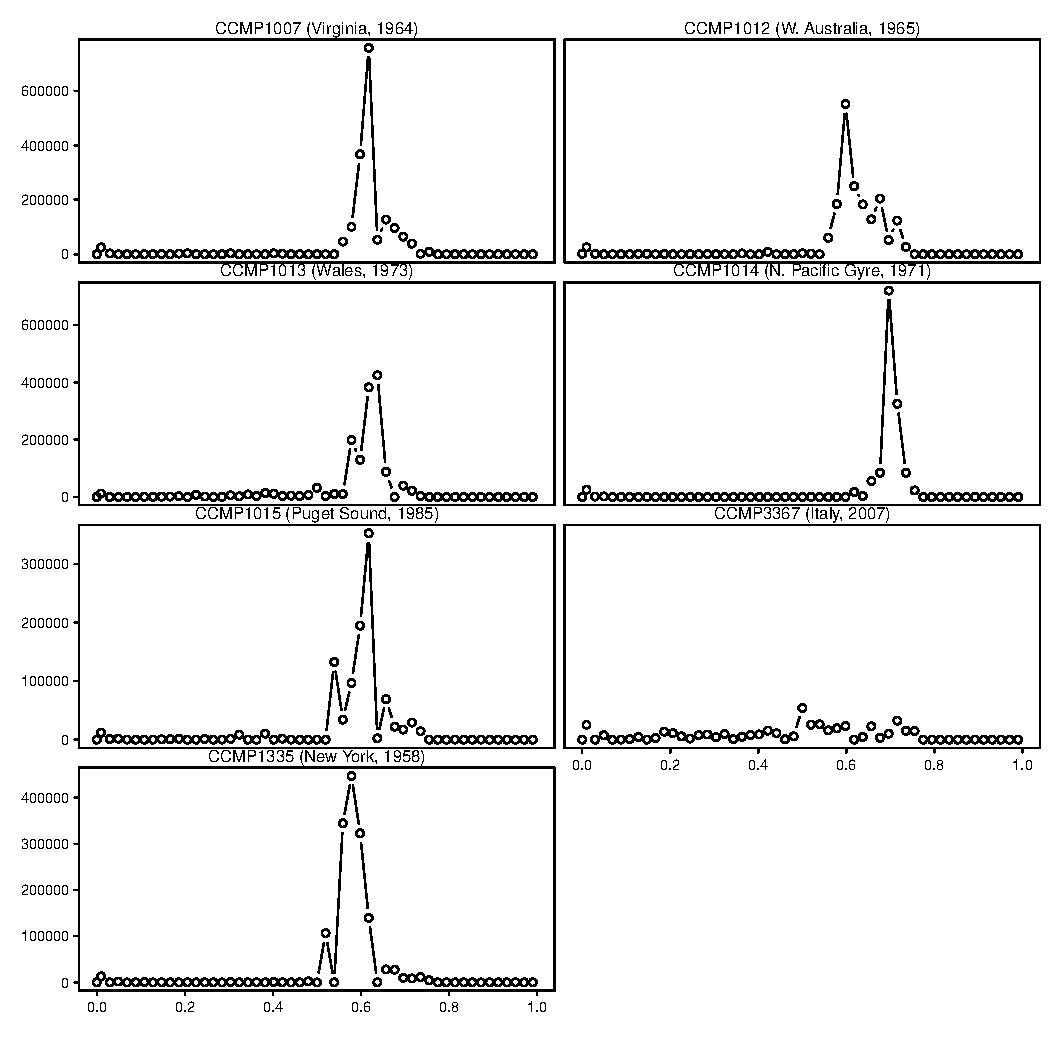
\includegraphics[width=\maxwidth]{figs-knitr/unnamed-chunk-31-1} 

}



\end{knitrout}

Observations: T-i-c is roughly reflected in peak heights, with Italy being most extreme. NY mode is $\approx 0.59$,  1007, 1012 and 1015 at $\approx 0.61$, 1013 at $\approx 0.63$, gyre at $\approx 0.71$  (and Italy has no clear peak).  If these are really hemizygous deletions, why are they not at 0.5?  Some regions may simply be at the low end of normal fluctuation in coverage, not deletions at all.  Additionally, discrete bin boundaries used by CNVnator may tend to include extraneous stuff at the ends of each interval.  Both effects should be reduced for longer regions; is there a length trend?

\begin{knitrout}\footnotesize
\definecolor{shadecolor}{rgb}{0.969, 0.969, 0.969}\color{fgcolor}\begin{kframe}
\begin{alltt}
\hlstd{plt.hemi.frac.by.len} \hlkwb{<-} \hlkwa{function}\hlstd{(}\hlkwc{logx}\hlstd{=F,}\hlkwc{sqrtx}\hlstd{=T)\{}
  \hlstd{opar} \hlkwb{<-} \hlkwd{par}\hlstd{(}\hlkwc{mfrow}\hlstd{=}\hlkwd{c}\hlstd{(}\hlnum{4}\hlstd{,}\hlnum{2}\hlstd{),}\hlkwc{mar}\hlstd{=}\hlkwd{c}\hlstd{(}\hlnum{0}\hlstd{,}\hlnum{0}\hlstd{,}\hlnum{1}\hlstd{,}\hlnum{.5}\hlstd{),}\hlkwc{oma}\hlstd{=}\hlkwd{c}\hlstd{(}\hlnum{3}\hlstd{,}\hlnum{4}\hlstd{,}\hlnum{1}\hlstd{,}\hlnum{0}\hlstd{));} \hlkwd{on.exit}\hlstd{(}\hlkwd{par}\hlstd{(opar))}
  \hlstd{xmx} \hlkwb{<-} \hlkwd{max}\hlstd{(cnvv}\hlopt{$}\hlstd{length)}
  \hlkwa{for}\hlstd{(i} \hlkwa{in} \hlnum{1}\hlopt{:}\hlnum{7}\hlstd{)\{}
    \hlstd{pick} \hlkwb{<-} \hlkwd{as.character}\hlstd{(cnvv}\hlopt{$}\hlstd{strain)} \hlopt{==} \hlstd{strain.names[i]}
    \hlstd{x} \hlkwb{<-} \hlstd{cnvv}\hlopt{$}\hlstd{length[pick]}
    \hlstd{xlm} \hlkwb{<-} \hlstd{xmx}
    \hlstd{xlb} \hlkwb{<-} \hlstr{'cnvv$length'}
    \hlkwa{if}\hlstd{(logx) \{}
      \hlstd{x} \hlkwb{<-} \hlkwd{log2}\hlstd{(x)}
      \hlstd{xlm} \hlkwb{<-} \hlkwd{log2}\hlstd{(xmx)}
      \hlstd{xlb} \hlkwb{<-} \hlstr{'log2(cnvv$length)'}
    \hlstd{\}} \hlkwa{else if}\hlstd{(sqrtx)\{}
      \hlstd{x} \hlkwb{<-} \hlkwd{sqrt}\hlstd{(x)}
      \hlstd{xlm} \hlkwb{<-} \hlkwd{sqrt}\hlstd{(xmx)}
      \hlstd{xlb} \hlkwb{<-} \hlstr{'sqrt(cnvv$length)'}
    \hlstd{\}}
    \hlkwd{eplot}\hlstd{(}\hlkwc{ylim}\hlstd{=}\hlkwd{c}\hlstd{(}\hlnum{0}\hlstd{,}\hlnum{1}\hlstd{),} \hlkwc{xlim}\hlstd{=}\hlkwd{c}\hlstd{(}\hlnum{0}\hlstd{,xlm),} \hlkwc{xlab}\hlstd{=xlb,} \hlkwc{ylab}\hlstd{=}\hlstr{'cov_ratio'}\hlstd{,}\hlkwc{main}\hlstd{=}\hlkwd{st.loc}\hlstd{(i,}\hlkwc{date}\hlstd{=T))}
    \hlkwd{points}\hlstd{(x, cnvv}\hlopt{$}\hlstd{cov_ratio[pick])}
    \hlkwd{abline}\hlstd{(}\hlkwc{h}\hlstd{=}\hlnum{0.6}\hlstd{,}\hlkwc{lwd}\hlstd{=}\hlnum{0.5}\hlstd{,}\hlkwc{col}\hlstd{=}\hlstr{'blue'}\hlstd{)}
    \hlkwa{if}\hlstd{(i}\hlopt{==}\hlnum{6}\hlstd{)\{}\hlkwd{addxaxis}\hlstd{()\}}
  \hlstd{\}}
\hlstd{\}}
\hlkwd{plt.hemi.frac.by.len}\hlstd{()}
\end{alltt}
\end{kframe}

{\centering 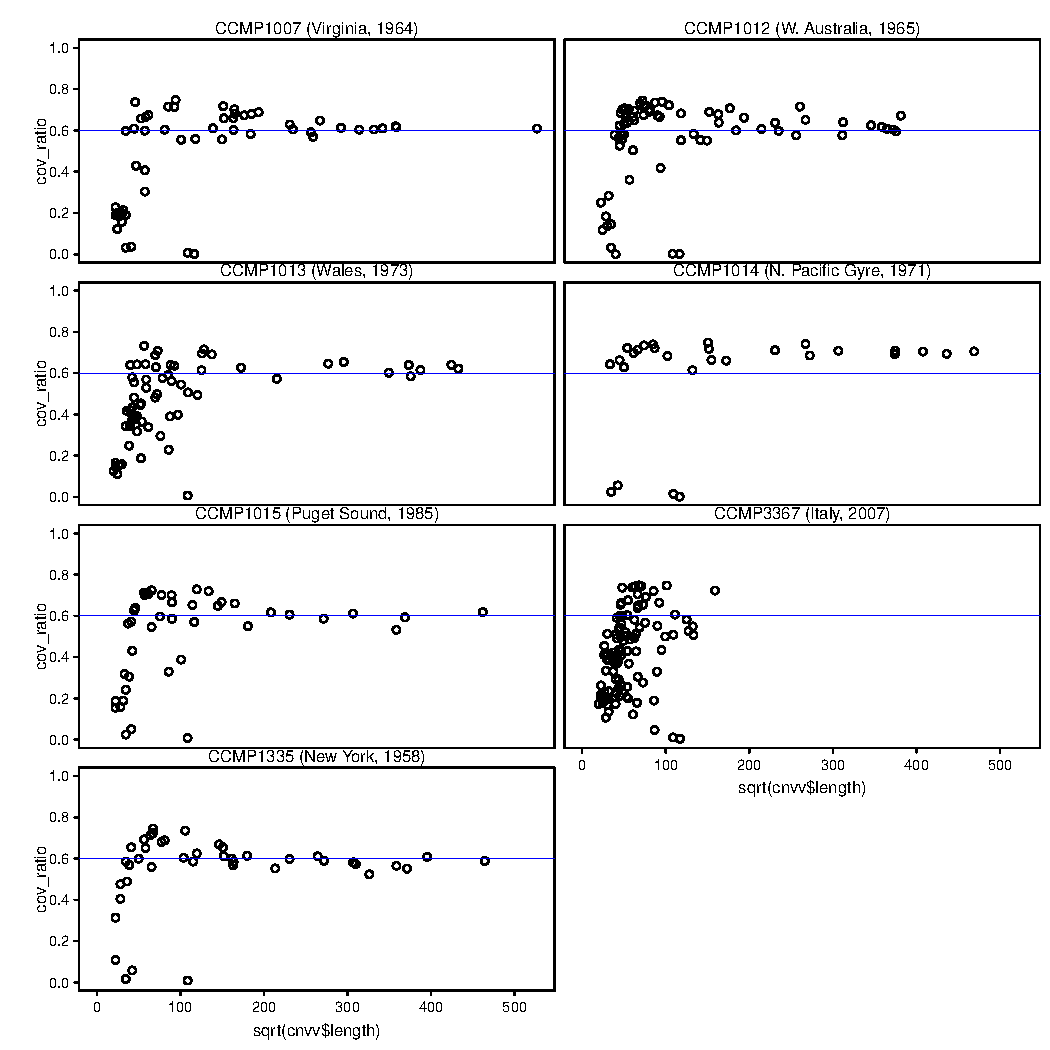
\includegraphics[width=\maxwidth]{figs-knitr/unnamed-chunk-32-1} 

}



\end{knitrout}

I'd say, no.  Coverage ratio is variable below 10k, but flat near 0.6 above that.  (A bit higher in Gyre, again either a symptom of increased noise or increased diversity in Gyre.)  Another possibility is that, just as coverage is low across SNPs due to a mapping bias against non-reference positions, there is a counter-trend \emph{towards} accepting erroneous reads that happen to \emph{match} the reference.  I suppose it is possible that this has inflated the ratio to 0.6 (or a bit more in Gyre, if it is noisier).  This one would imply a rather startling rate of erroneous reads:  If the number of ``correct'' reads across a diploid section averages $x$, and some additional fraction $\epsilon x$ of erroneous reads map there too, then 
  $$ \frac{x/2+\epsilon x}{x+\epsilon x}=0.6,$$ 
implying $\epsilon=1/4$. 

Another possibility is that stochasticity contributes:  fluctuation around average read count of 0.5 can't fall below zero, but can rise above 1.0, which might tend to inflate the observed average.  Additionally, duplicated or non-hemi regions embedded in/sandwiched between two long hemi regions might, if short, not be properly split by CNVnator, inflating the average.  Another contributor is that a sigificant proportion of hemizygousity will lower the genomic coverage average against which \verb|cov_ratio| is measured.  (This effect should be strongest on the older strains, where deletion appears most widespread, but I don't see an obvious trend in that direction.  Although we didn't look, I wouldn't be surprised to see duplications increasing with age, too, which would partially offset this effect. UPDATE: I did take a quick look; 1.5x and 2x appear to increase with age, and there's a lot around 1.5x but relatively little at 2x or above, e.g. an average of about 0.5 Mb between 1.7x and 2.3x, vs at least twice that in hemizygous regions.) 

Big NY deletions:

\begin{knitrout}\footnotesize
\definecolor{shadecolor}{rgb}{0.969, 0.969, 0.969}\color{fgcolor}\begin{kframe}
\begin{alltt}
\hlstd{pick} \hlkwb{<-} \hlstd{cnvv}\hlopt{$}\hlstd{strain} \hlopt{==} \hlstr{'tp1335'} \hlopt{&} \hlstd{cnvv}\hlopt{$}\hlstd{length} \hlopt{>} \hlnum{40000}
\hlkwd{sum}\hlstd{(pick)}
\end{alltt}
\begin{verbatim}
# [1] 11
\end{verbatim}
\begin{alltt}
\hlstd{pi.length} \hlkwb{<-} \hlkwd{order}\hlstd{(cnvv}\hlopt{$}\hlstd{length)}
\hlstd{cnvv[pi.length,][pick[pi.length],]}
\end{alltt}
\begin{verbatim}
#      strain       chr   start     end length filtered     type cov_ratio  dup_frac
# 2114 tp1335      Chr2 2399101 2444700  45600    FALSE CNVnator  0.551821 0.0385429
# 2117 tp1335      Chr2 2582101 2635300  53200    FALSE CNVnator  0.598177 0.0706814
# 2274 tp1335 Chr19a_19  479301  549200  69900    FALSE CNVnator  0.610449 0.0569739
# 2161 tp1335      Chr6  272601  346500  73900    FALSE CNVnator  0.588544 0.0702023
# 2159 tp1335      Chr6  174501  268500  94000    FALSE CNVnator  0.581503 0.0364507
# 2310 tp1335     Chr23       1   96000  96000    FALSE CNVnator  0.572798 0.0462243
# 2290 tp1335     Chr20  621601  728000 106400    FALSE CNVnator  0.522981 0.1220760
# 2115 tp1335      Chr2 2448101 2576700 128600    FALSE CNVnator  0.565107 0.0294771
# 2269 tp1335 Chr19a_19  281201  419000 137800    FALSE CNVnator  0.550752 0.0298223
# 2157 tp1335      Chr6    9601  165900 156300    FALSE CNVnator  0.607829 0.0390458
# 2267 tp1335 Chr19a_19   62201  277800 215600    FALSE CNVnator  0.587722 0.0744552
\end{verbatim}
\end{kframe}
\end{knitrout}

\section{Examples}

Looking at some examples:

\begin{knitrout}\footnotesize
\definecolor{shadecolor}{rgb}{0.969, 0.969, 0.969}\color{fgcolor}\begin{kframe}
\begin{alltt}
\hlcom{# look up a coord in hemi table}
\hlstd{hemi.row} \hlkwb{<-} \hlkwa{function}\hlstd{(}\hlkwc{coord}\hlstd{,}\hlkwc{h.t}\hlstd{=hemi.tab)\{}
  \hlstd{r} \hlkwb{<-} \hlkwd{match}\hlstd{(coord,}\hlkwd{rownames}\hlstd{(h.t))}
  \hlkwa{if}\hlstd{(}\hlkwd{is.na}\hlstd{(r))\{}

  \hlstd{\}}
\hlstd{\}}
\hlcom{# rows = range of row indices e.g. 18:24, or pair of row names c('Chr10:104501','Chr10:104501')}
\hlcom{# alt.win is start if first to end of 2nd; print tab for a row earlier to row later}
\hlstd{hemi.chunk} \hlkwb{<-} \hlkwa{function}\hlstd{(}\hlkwc{rows}\hlstd{,}\hlkwc{strains}\hlstd{=}\hlkwd{c}\hlstd{(}\hlnum{7}\hlstd{,}\hlnum{1}\hlopt{:}\hlnum{6}\hlstd{),}\hlkwc{margin}\hlstd{=}\hlnum{1000}\hlstd{,}\hlkwc{ymax}\hlstd{=}\hlnum{250}\hlstd{,} \hlkwc{h.t}\hlstd{=hemi.tab)\{}
  \hlkwa{if}\hlstd{(}\hlkwd{length}\hlstd{(strains)}\hlopt{>}\hlnum{1}\hlstd{)\{}
    \hlstd{opar} \hlkwb{<-} \hlkwd{par}\hlstd{(}\hlkwc{ask}\hlstd{=T);} \hlkwd{on.exit}\hlstd{(}\hlkwd{par}\hlstd{(opar))}
  \hlstd{\}}
  \hlkwa{if}\hlstd{(}\hlkwd{is.numeric}\hlstd{(rows))\{}
    \hlstd{j} \hlkwb{<-} \hlkwd{min}\hlstd{(rows)}
    \hlstd{k} \hlkwb{<-} \hlkwd{max}\hlstd{(rows)}
  \hlstd{\}} \hlkwa{else} \hlstd{\{}
    \hlstd{j} \hlkwb{<-} \hlkwd{match}\hlstd{(rows[}\hlnum{1}\hlstd{],}\hlkwd{rownames}\hlstd{(h.t))}
    \hlstd{k} \hlkwb{<-} \hlkwd{match}\hlstd{(rows[}\hlkwd{length}\hlstd{(rows)],}\hlkwd{rownames}\hlstd{(h.t))}
    \hlkwd{cat}\hlstd{(}\hlstr{'Rows'}\hlstd{,j,}\hlstr{':'}\hlstd{,k,}\hlstr{'\textbackslash{}n'}\hlstd{)}
  \hlstd{\}}
  \hlkwd{print}\hlstd{(h.t[}\hlkwd{max}\hlstd{(}\hlnum{1}\hlstd{,j}\hlopt{-}\hlnum{1}\hlstd{)}\hlopt{:}\hlkwd{min}\hlstd{(}\hlkwd{nrow}\hlstd{(h.t),k}\hlopt{+}\hlnum{1}\hlstd{),],} \hlkwc{digits}\hlstd{=}\hlnum{3}\hlstd{)}
  \hlstd{start} \hlkwb{<-} \hlkwd{chrloc2g}\hlstd{(}\hlkwd{list}\hlstd{(h.t}\hlopt{$}\hlstd{chr[j], h.t}\hlopt{$}\hlstd{start[j]))}
  \hlstd{end}   \hlkwb{<-} \hlkwd{chrloc2g}\hlstd{(}\hlkwd{list}\hlstd{(h.t}\hlopt{$}\hlstd{chr[k], h.t}\hlopt{$}\hlstd{end[k]))}
  \hlkwa{for}\hlstd{(i} \hlkwa{in} \hlstd{strains)\{}
    \hlcom{#cat('x=',(start+end)/2,'width=',(end-start)/2+margin,'\textbackslash{}n')}
    \hlkwd{seechunk}\hlstd{(i,}\hlkwd{ceiling}\hlstd{((start}\hlopt{+}\hlstd{end)}\hlopt{/}\hlnum{2}\hlstd{),}\hlkwc{width}\hlstd{=}\hlkwd{ceiling}\hlstd{((end}\hlopt{-}\hlstd{start)}\hlopt{/}\hlnum{2}\hlstd{)}\hlopt{+}\hlstd{margin,}
             \hlkwc{alt.win}\hlstd{=}\hlkwd{c}\hlstd{(start,end),}\hlkwc{ymax}\hlstd{=ymax)}
  \hlstd{\}}
\hlstd{\}}
\end{alltt}
\end{kframe}
\end{knitrout}

Start with big NY deletions.  The first is about 45k long.  As expected for a hemizygous region, it is essentially SNP-free in NY (there are 2 or 3 called SNPs, all with very low non-reference read counts).
An even longer region is deleted in 1007 and 1012, and each has about 5 called SNPs with substantial nonreference counts (possibly at shared positions), plus 2--3 others with low counts.  In other words, all 3 strains appear to be hemizygous here, and to share the same haplotype, give or take a handful of nucleotides.  1014 and 1015 have normal coverage, but few SNPs (4--7)---essentially homozygous for the NY haplotype.  Italy and Wales have normal coverage and many SNPs, although the Italy's SNPs are somewhat patchy.  Italian and Welsh SNPs have a complex sharing pattern, with a majority of Wales below 0.5 nonref frac, and IT the opposite; many of the high nonref frac are shared, but many of all frequencies are private to each strain (see pairs plot below).

\begin{knitrout}\footnotesize
\definecolor{shadecolor}{rgb}{0.969, 0.969, 0.969}\color{fgcolor}\begin{kframe}
\begin{alltt}
\hlkwd{hemi.chunk}\hlstd{(}\hlkwd{c}\hlstd{(}\hlstr{'Chr2:2399101'}\hlstd{,}\hlstr{'Chr2:2444601'}\hlstd{),}\hlkwc{margin}\hlstd{=}\hlnum{5000}\hlstd{)}
\end{alltt}
\begin{verbatim}
# Rows 340 : 341 
#               chr   start     end length tp1007 tp1012 tp1013 tp1014 tp1015 IT tp1335 pattern
# Chr2:2348101 Chr2 2348101 2399100  51000  0.604  0.576     NA     NA     NA NA     NA     140
# Chr2:2399101 Chr2 2399101 2444600  45500  0.604  0.576     NA     NA     NA NA  0.552     141
# Chr2:2444601 Chr2 2444601 2444700    100  0.604     NA     NA     NA     NA NA  0.552     101
# Chr2:2444701 Chr2 2444701 2446700   2000  0.604     NA     NA     NA     NA NA     NA     100
\end{verbatim}
\end{kframe}

{\centering 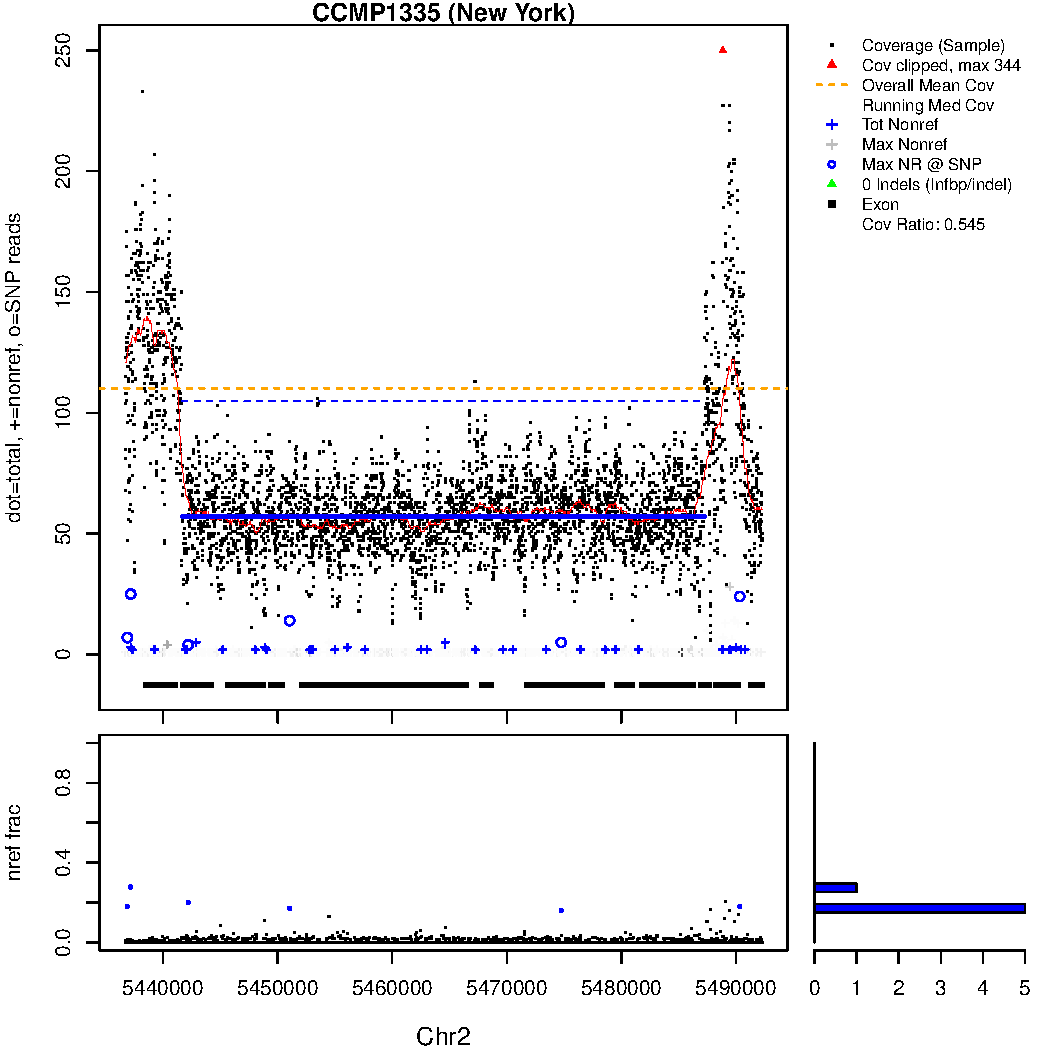
\includegraphics[width=\maxwidth]{figs-knitr/unnamed-chunk-35-1} 
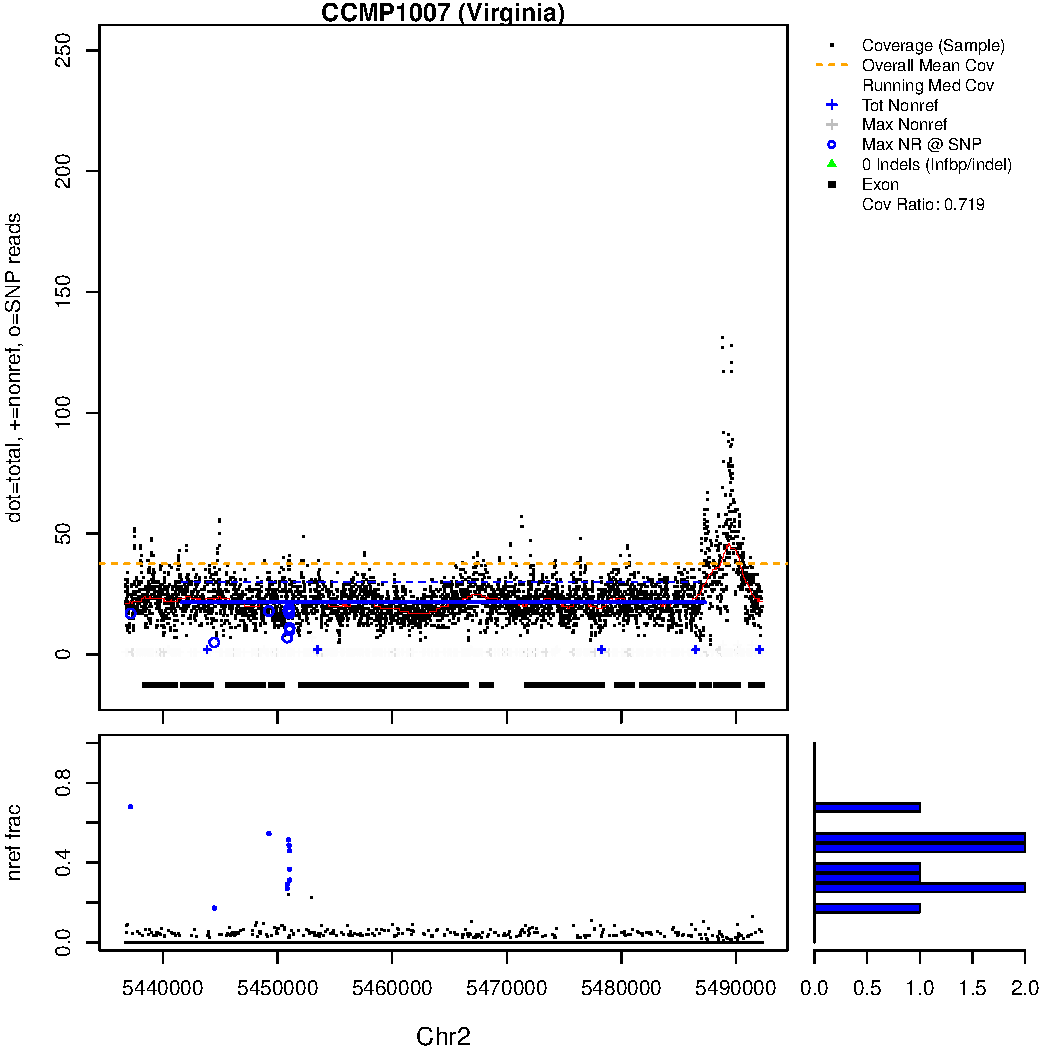
\includegraphics[width=\maxwidth]{figs-knitr/unnamed-chunk-35-2} 
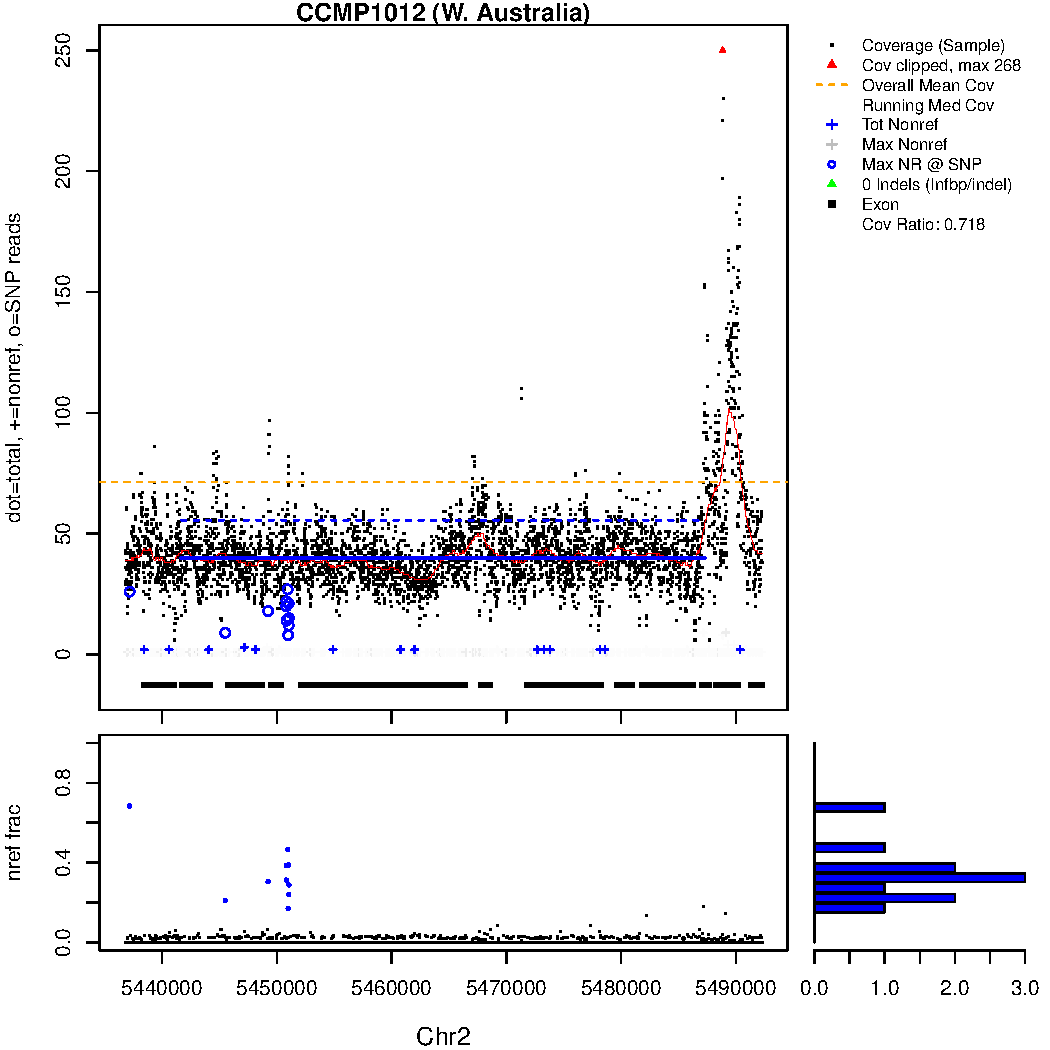
\includegraphics[width=\maxwidth]{figs-knitr/unnamed-chunk-35-3} 
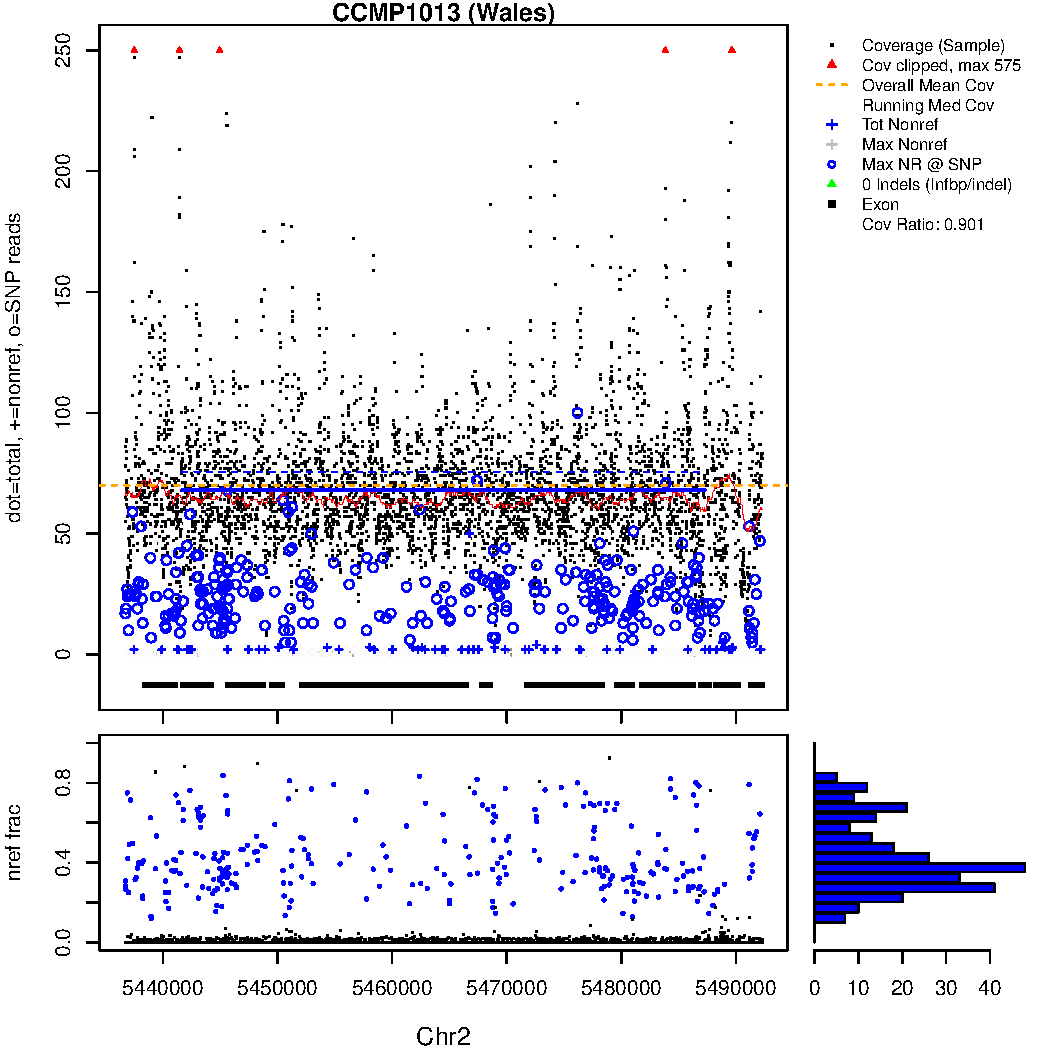
\includegraphics[width=\maxwidth]{figs-knitr/unnamed-chunk-35-4} 
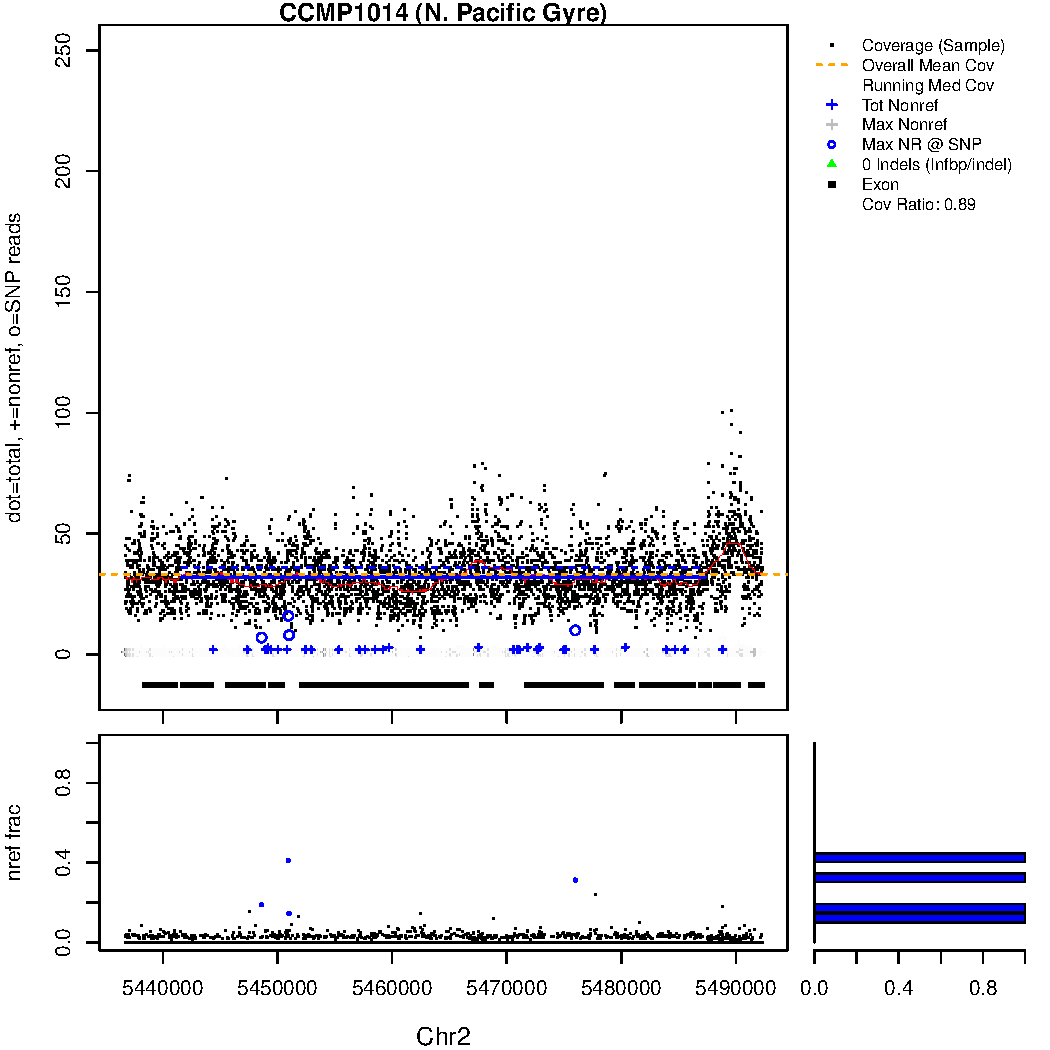
\includegraphics[width=\maxwidth]{figs-knitr/unnamed-chunk-35-5} 
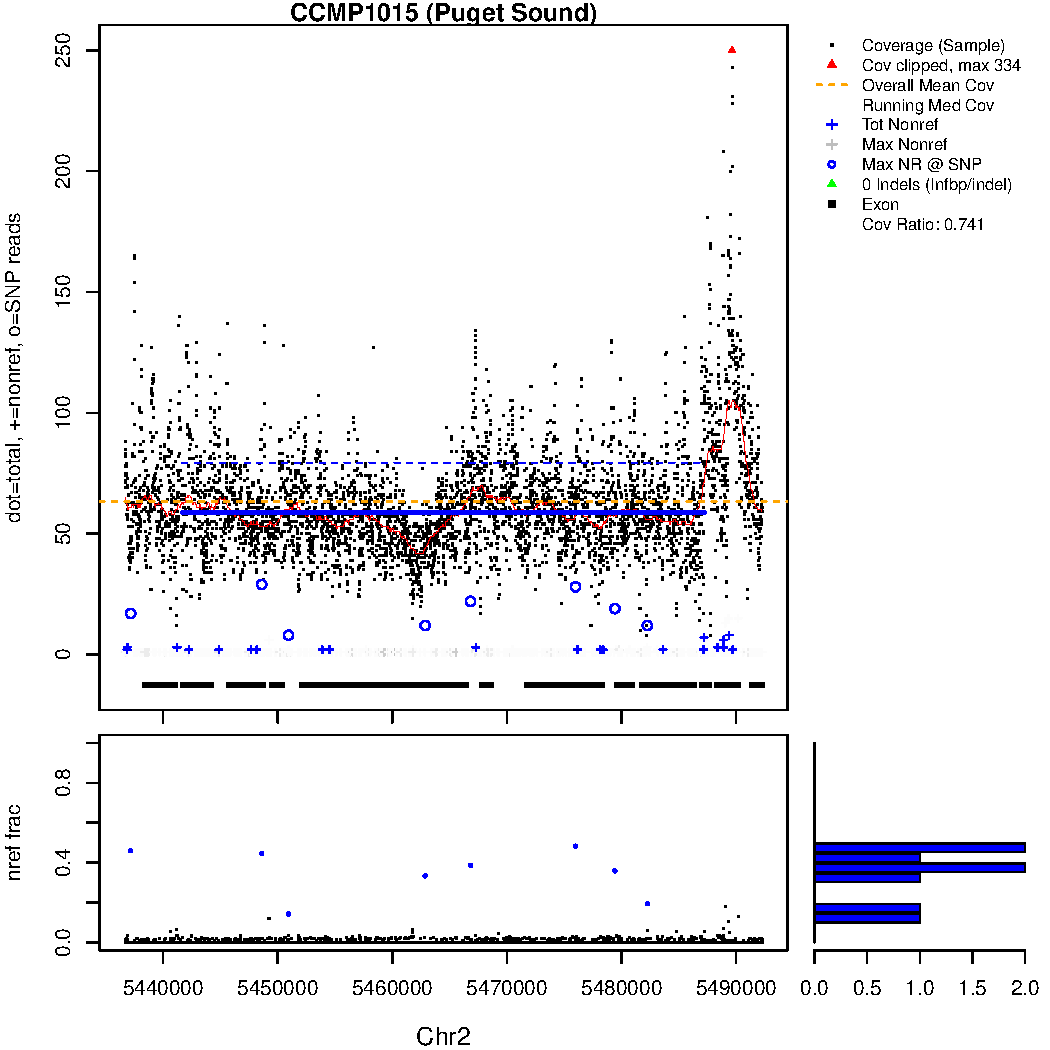
\includegraphics[width=\maxwidth]{figs-knitr/unnamed-chunk-35-6} 
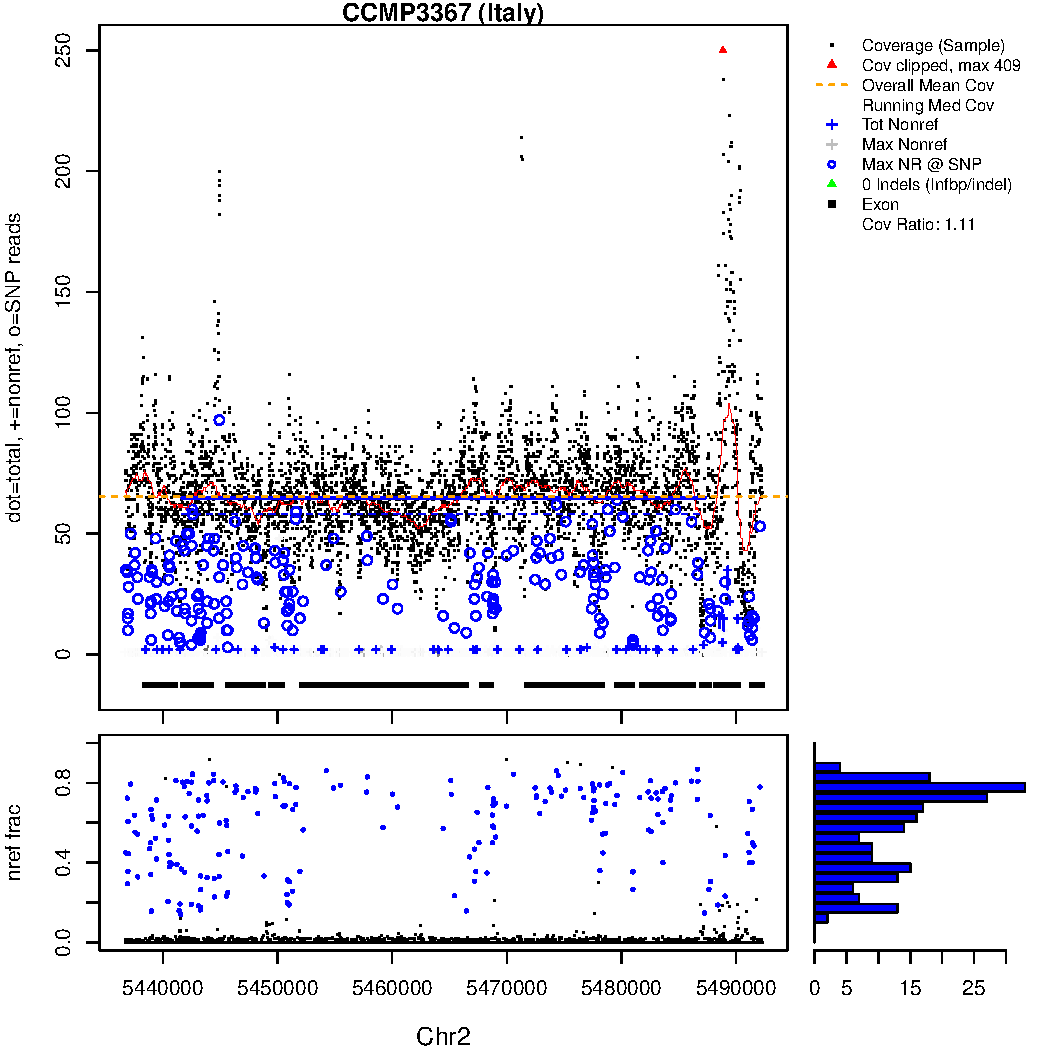
\includegraphics[width=\maxwidth]{figs-knitr/unnamed-chunk-35-7} 

}



\end{knitrout}

pairs plot of same region:

\begin{knitrout}\footnotesize
\definecolor{shadecolor}{rgb}{0.969, 0.969, 0.969}\color{fgcolor}\begin{kframe}
\begin{alltt}
\hlkwd{nrf.pairs}\hlstd{(}\hlkwc{mask}\hlstd{=}\hlkwd{seg.mask}\hlstd{(}\hlnum{5440000}\hlstd{,}\hlnum{5500000}\hlstd{))}
\end{alltt}
\end{kframe}

{\centering 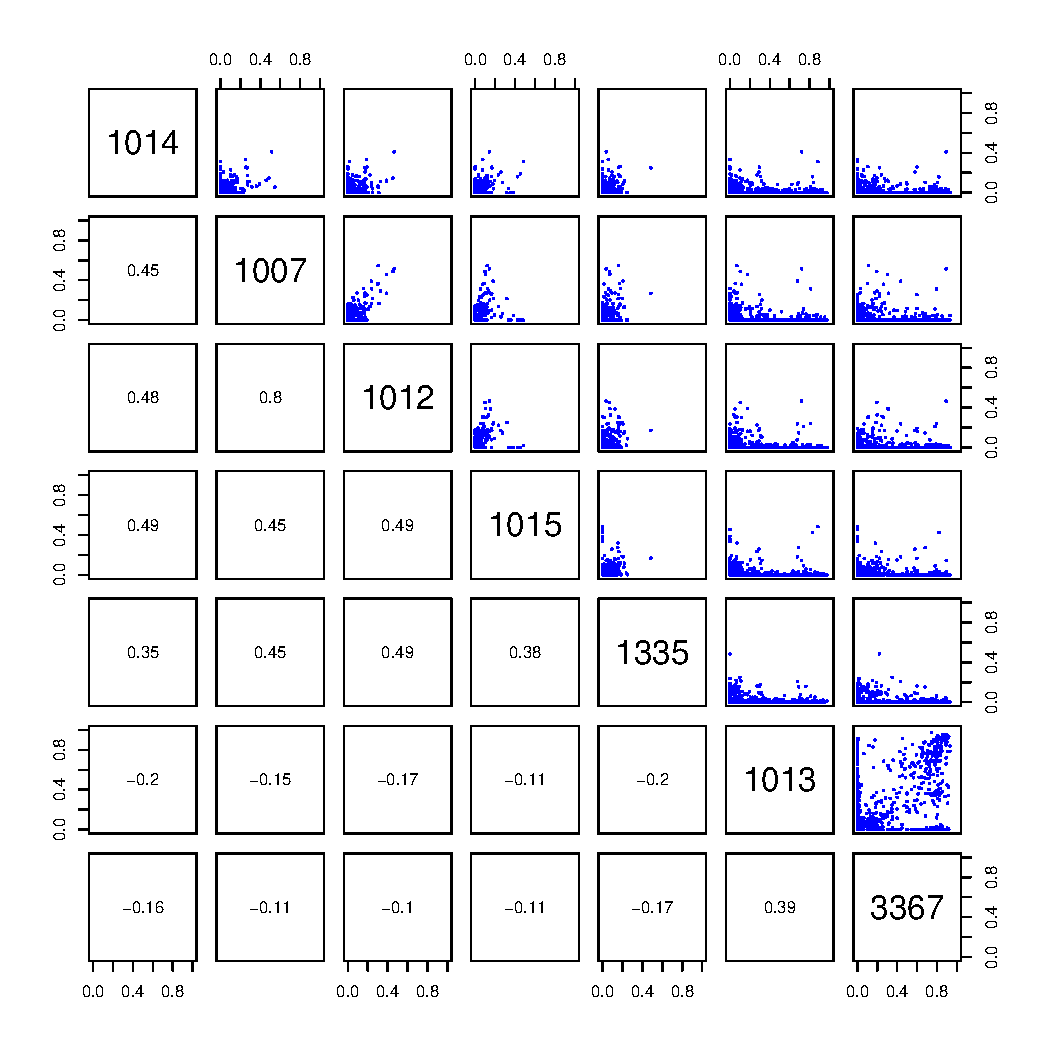
\includegraphics[width=\maxwidth]{figs-knitr/unnamed-chunk-36-1} 

}



\end{knitrout}


Extending that, we see that, with a few relatively short interruptions (perhaps duplicated regions), the NY deletion essentially runs to the end of Chr2, although not consistently called by CNVnator, and the described pattern above applies to the whole region ($\approx 400$K), \emph{except}, 1014 and 1015 share a region of about 100k that is very SNPy.

\begin{knitrout}\footnotesize
\definecolor{shadecolor}{rgb}{0.969, 0.969, 0.969}\color{fgcolor}\begin{kframe}
\begin{alltt}
\hlkwd{hemi.chunk}\hlstd{(}\hlnum{338}\hlopt{:}\hlnum{366}\hlstd{,}\hlkwc{margin}\hlstd{=}\hlnum{20000}\hlstd{)}
\end{alltt}
\begin{verbatim}
#               chr   start     end length tp1007 tp1012 tp1013 tp1014 tp1015    IT tp1335 pattern
# Chr2:2330601 Chr2 2330601 2347700  17100     NA     NA     NA     NA     NA    NA     NA     000
# Chr2:2347701 Chr2 2347701 2348100    400     NA  0.576     NA     NA     NA    NA     NA     040
# Chr2:2348101 Chr2 2348101 2399100  51000  0.604  0.576     NA     NA     NA    NA     NA     140
# Chr2:2399101 Chr2 2399101 2444600  45500  0.604  0.576     NA     NA     NA    NA  0.552     141
# Chr2:2444601 Chr2 2444601 2444700    100  0.604     NA     NA     NA     NA    NA  0.552     101
# Chr2:2444701 Chr2 2444701 2446700   2000  0.604     NA     NA     NA     NA    NA     NA     100
# Chr2:2446701 Chr2 2446701 2447800   1100     NA     NA     NA     NA     NA    NA     NA     000
# Chr2:2447801 Chr2 2447801 2448100    300     NA     NA     NA     NA     NA 0.422     NA     002
# Chr2:2448101 Chr2 2448101 2448600    500  0.616  0.617     NA     NA     NA 0.422  0.565     143
# Chr2:2448601 Chr2 2448601 2555700 107100  0.616  0.617     NA     NA     NA    NA  0.565     141
# Chr2:2555701 Chr2 2555701 2576700  21000  0.616  0.617     NA     NA  0.648    NA  0.565     145
# Chr2:2576701 Chr2 2576701 2582000   5300     NA     NA     NA     NA     NA    NA     NA     000
# Chr2:2582001 Chr2 2582001 2582100    100  0.629  0.637     NA     NA     NA    NA     NA     140
# Chr2:2582101 Chr2 2582101 2594100  12000  0.629  0.637     NA  0.711  0.606    NA  0.598     155
# Chr2:2594101 Chr2 2594101 2597700   3600  0.629  0.637     NA  0.711  0.606 0.738  0.598     157
# Chr2:2597701 Chr2 2597701 2635300  37600  0.629  0.637     NA  0.711  0.606    NA  0.598     155
# Chr2:2635301 Chr2 2635301 2638000   2700     NA     NA     NA     NA     NA    NA     NA     000
# Chr2:2638001 Chr2 2638001 2638100    100     NA     NA     NA     NA  0.660    NA     NA     004
# Chr2:2638101 Chr2 2638101 2648900  10800  0.702  0.722     NA     NA  0.660    NA  0.604     145
# Chr2:2648901 Chr2 2648901 2650900   2000  0.702     NA     NA     NA  0.660    NA     NA     104
# Chr2:2650901 Chr2 2650901 2651200    300  0.702     NA     NA     NA  0.660    NA  0.625     105
# Chr2:2651201 Chr2 2651201 2665200  14000  0.702  0.682     NA     NA  0.660    NA  0.625     145
# Chr2:2665201 Chr2 2665201 2676900  11700     NA     NA     NA     NA     NA    NA     NA     000
# Chr2:2676901 Chr2 2676901 2677000    100  0.717     NA     NA  0.748     NA    NA     NA     110
# Chr2:2677001 Chr2 2677001 2699300  22300  0.717     NA     NA  0.748  0.667    NA  0.654     115
# Chr2:2699301 Chr2 2699301 2699600    300  0.717     NA     NA  0.748     NA    NA  0.654     111
# Chr2:2699601 Chr2 2699601 2699800    200  0.717     NA     NA     NA     NA    NA  0.654     101
# Chr2:2699801 Chr2 2699801 2706700   6900     NA     NA     NA     NA     NA    NA     NA     000
# Chr2:2706701 Chr2 2706701 2707194    494     NA     NA  0.166     NA     NA    NA     NA     020
# Chr2:2707195 Chr2 2707195 2707200      6     NA     NA  0.166     NA     NA    NA     NA     020
# Chr2:2707201 Chr2 2707201 2707200      0     NA     NA     NA     NA     NA    NA     NA     000
\end{verbatim}
\end{kframe}

{\centering 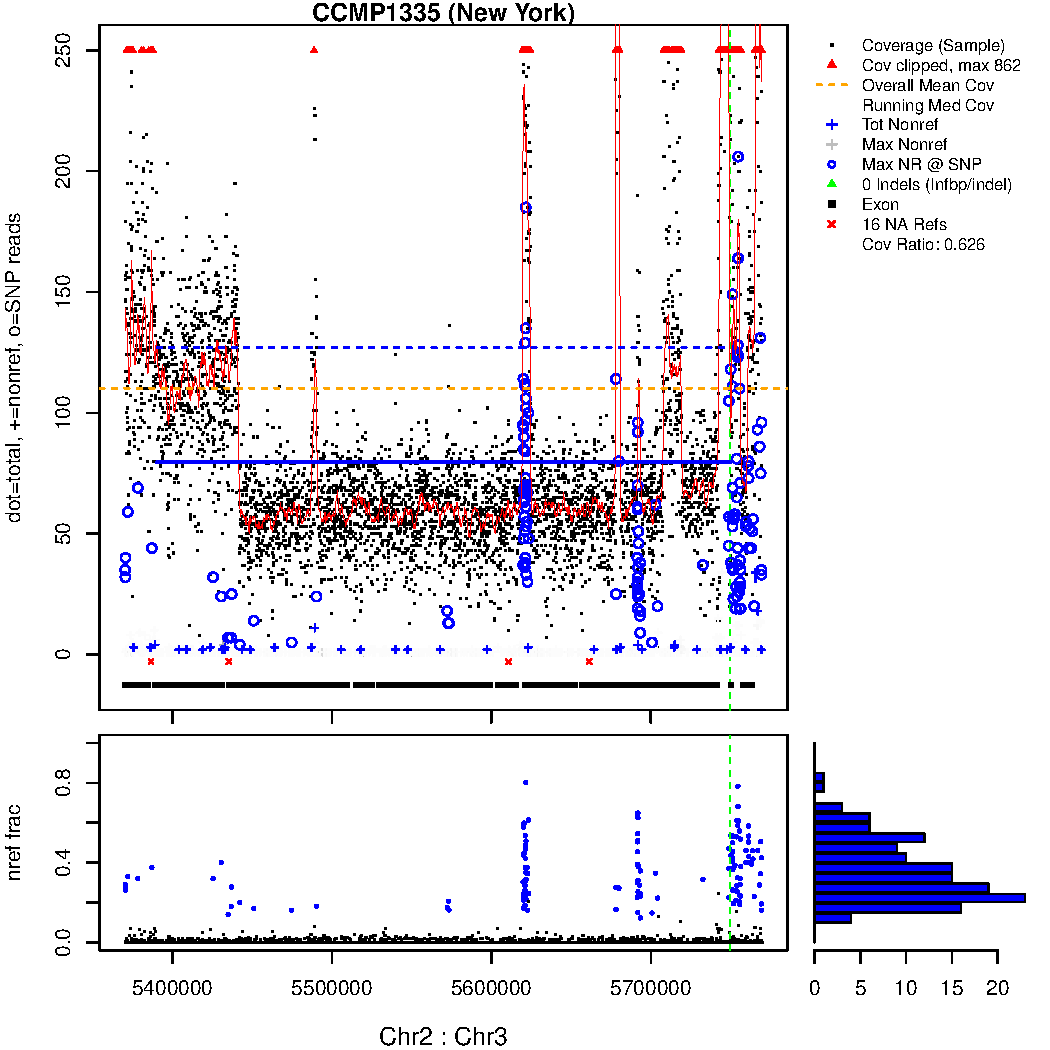
\includegraphics[width=\maxwidth]{figs-knitr/unnamed-chunk-37-1} 
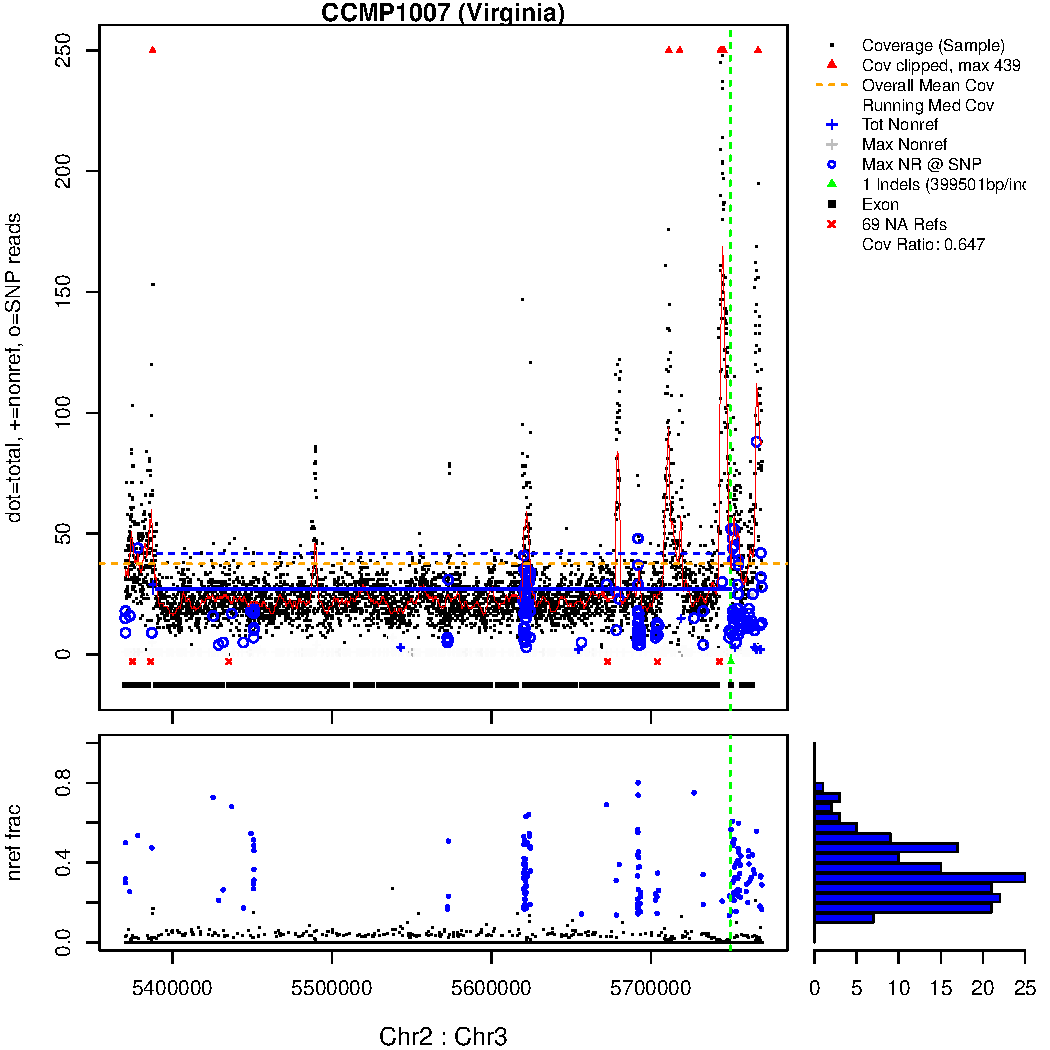
\includegraphics[width=\maxwidth]{figs-knitr/unnamed-chunk-37-2} 
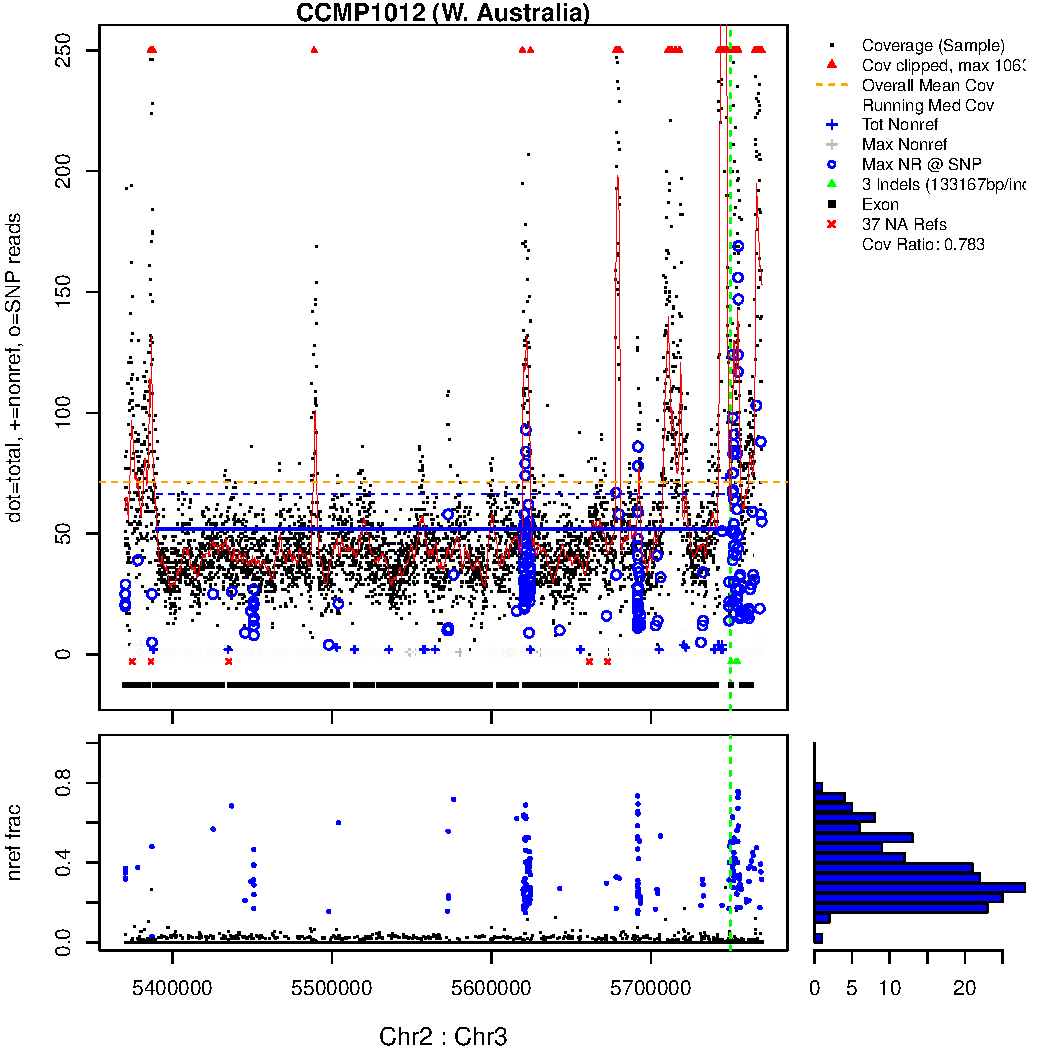
\includegraphics[width=\maxwidth]{figs-knitr/unnamed-chunk-37-3} 
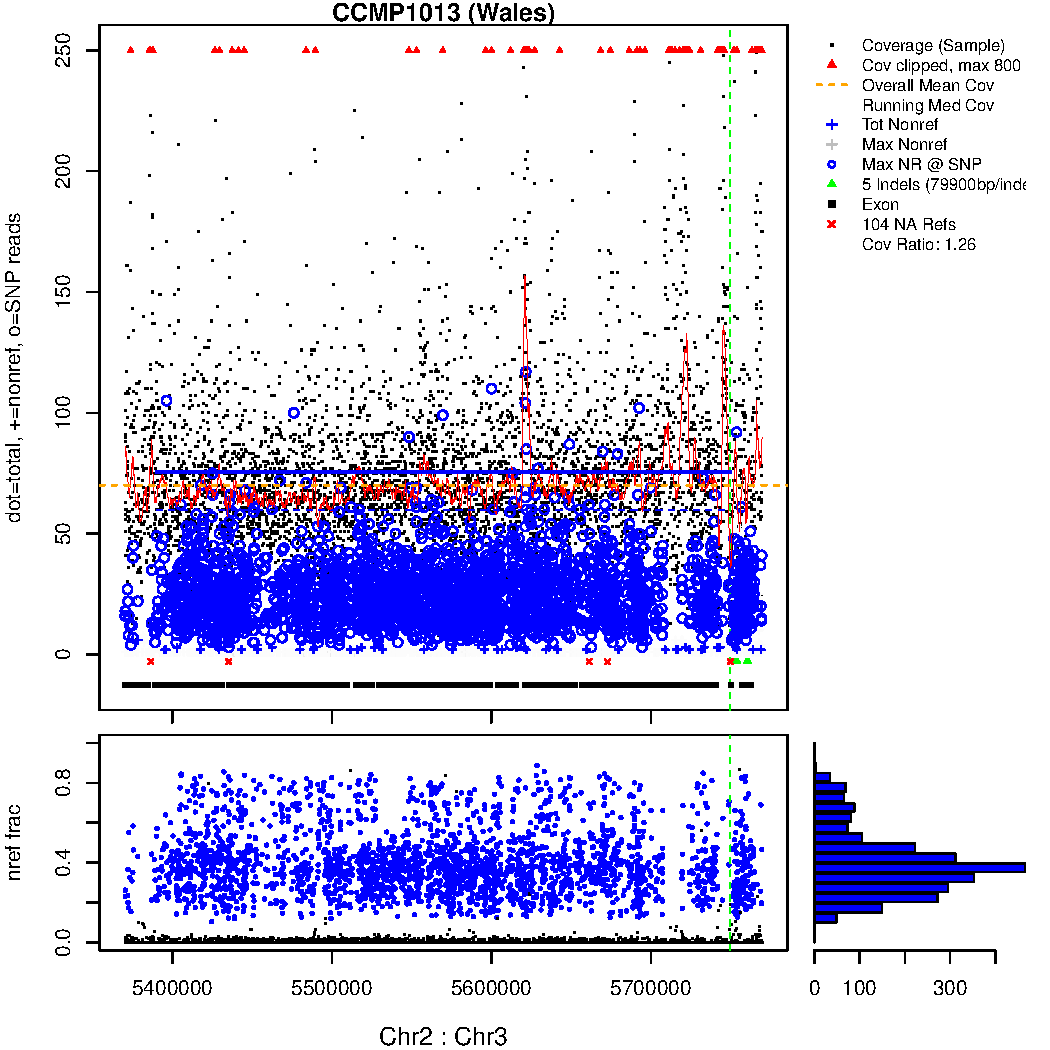
\includegraphics[width=\maxwidth]{figs-knitr/unnamed-chunk-37-4} 
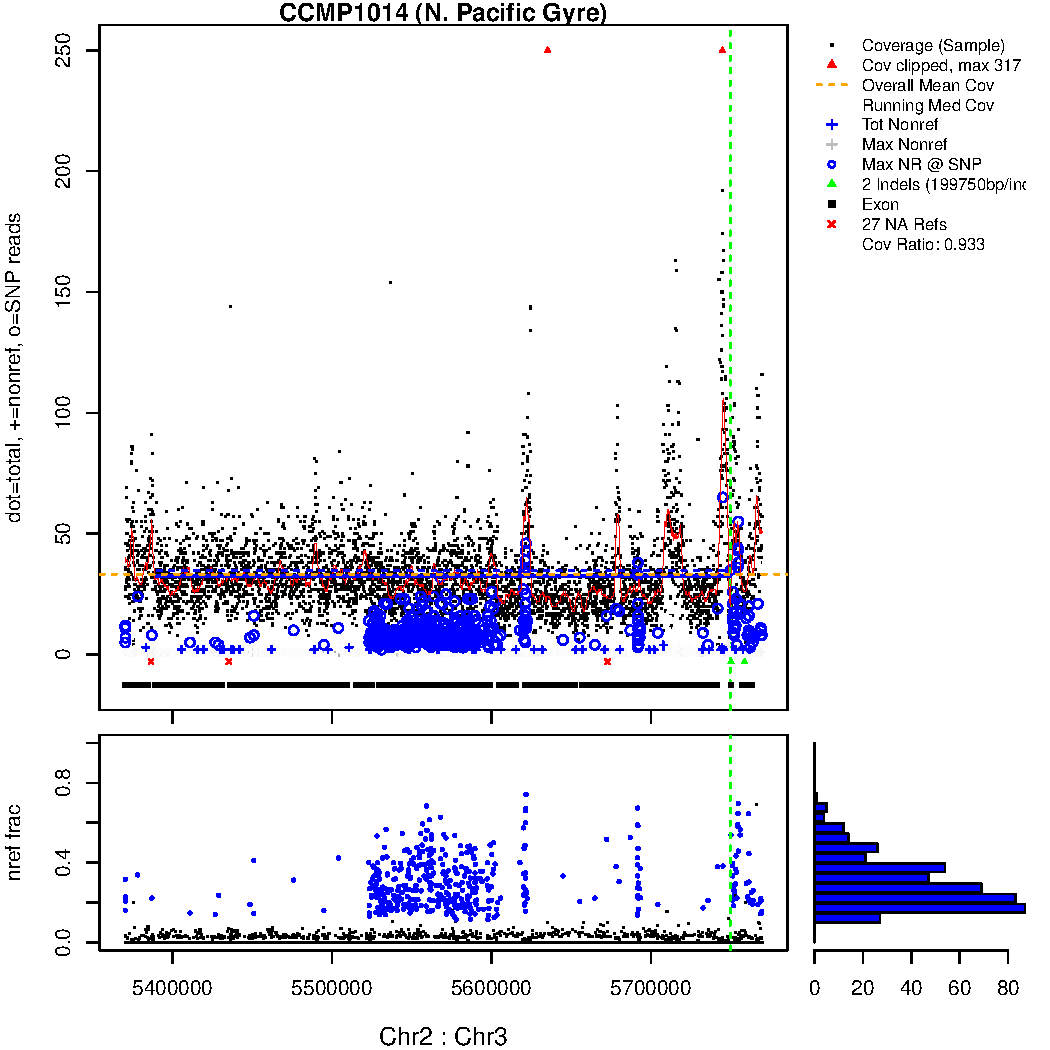
\includegraphics[width=\maxwidth]{figs-knitr/unnamed-chunk-37-5} 
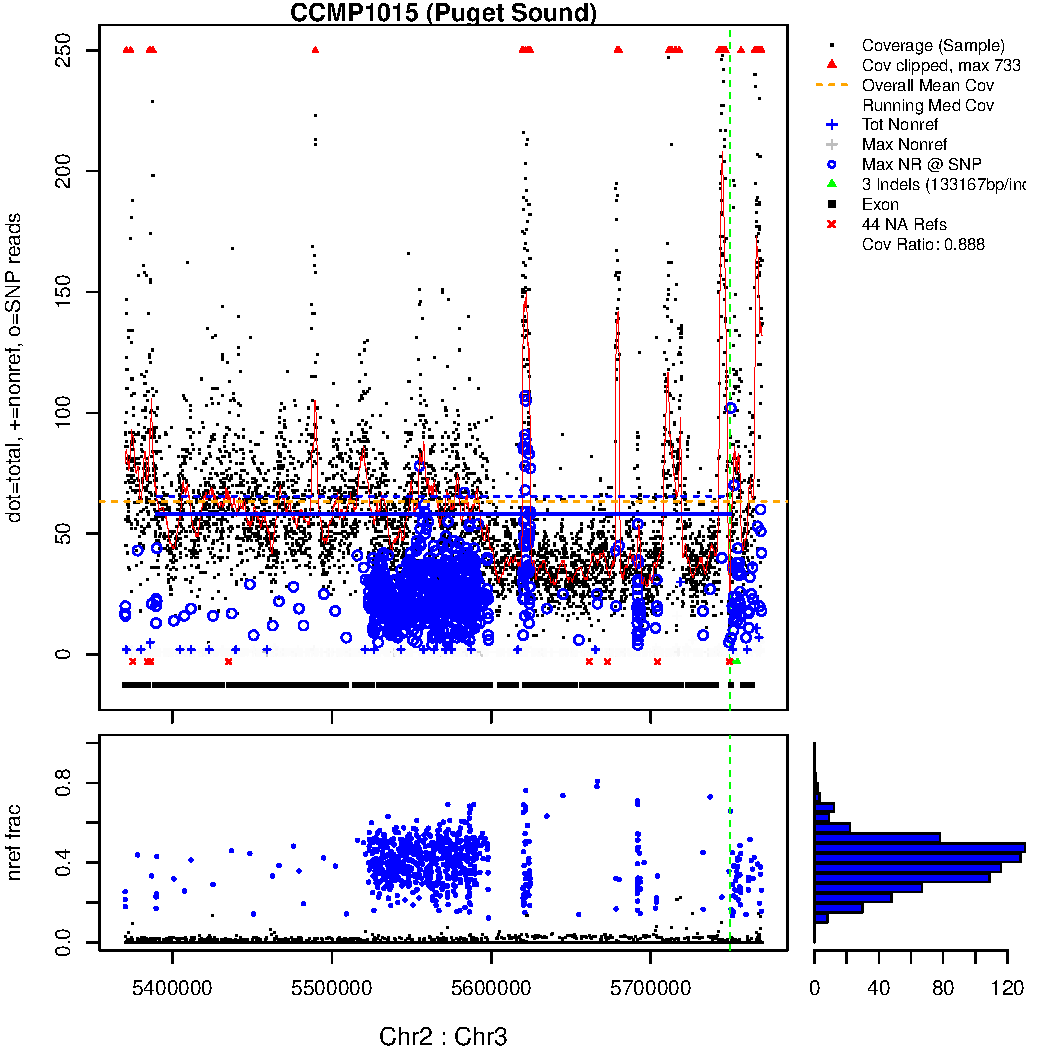
\includegraphics[width=\maxwidth]{figs-knitr/unnamed-chunk-37-6} 
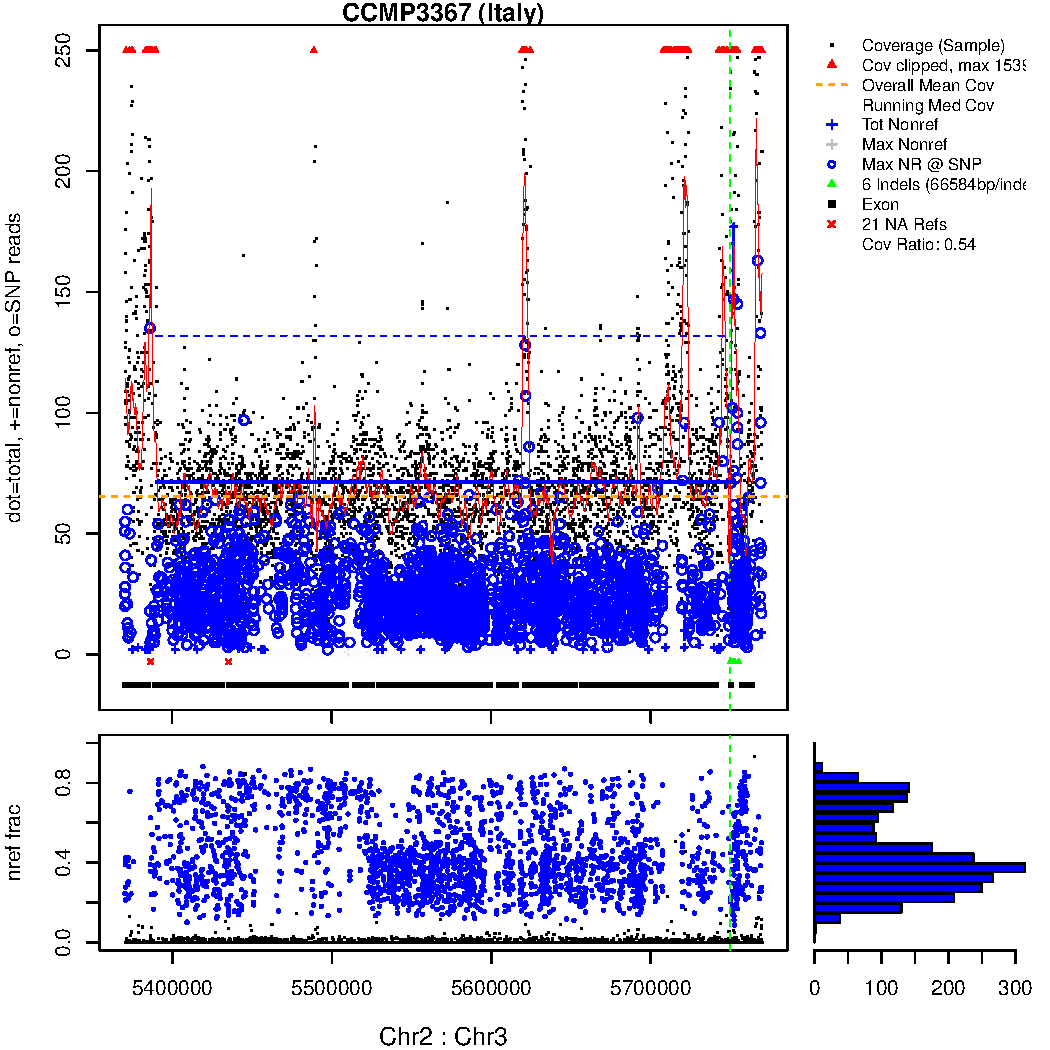
\includegraphics[width=\maxwidth]{figs-knitr/unnamed-chunk-37-7} 

}



\end{knitrout}

Pairs plot of same:
 
\begin{knitrout}\footnotesize
\definecolor{shadecolor}{rgb}{0.969, 0.969, 0.969}\color{fgcolor}\begin{kframe}
\begin{alltt}
\hlkwd{nrf.pairs}\hlstd{(}\hlkwc{mask}\hlstd{=}\hlkwd{seg.mask}\hlstd{(}\hlnum{5440000}\hlstd{,}\hlnum{5800000}\hlstd{))}
\end{alltt}
\end{kframe}

{\centering 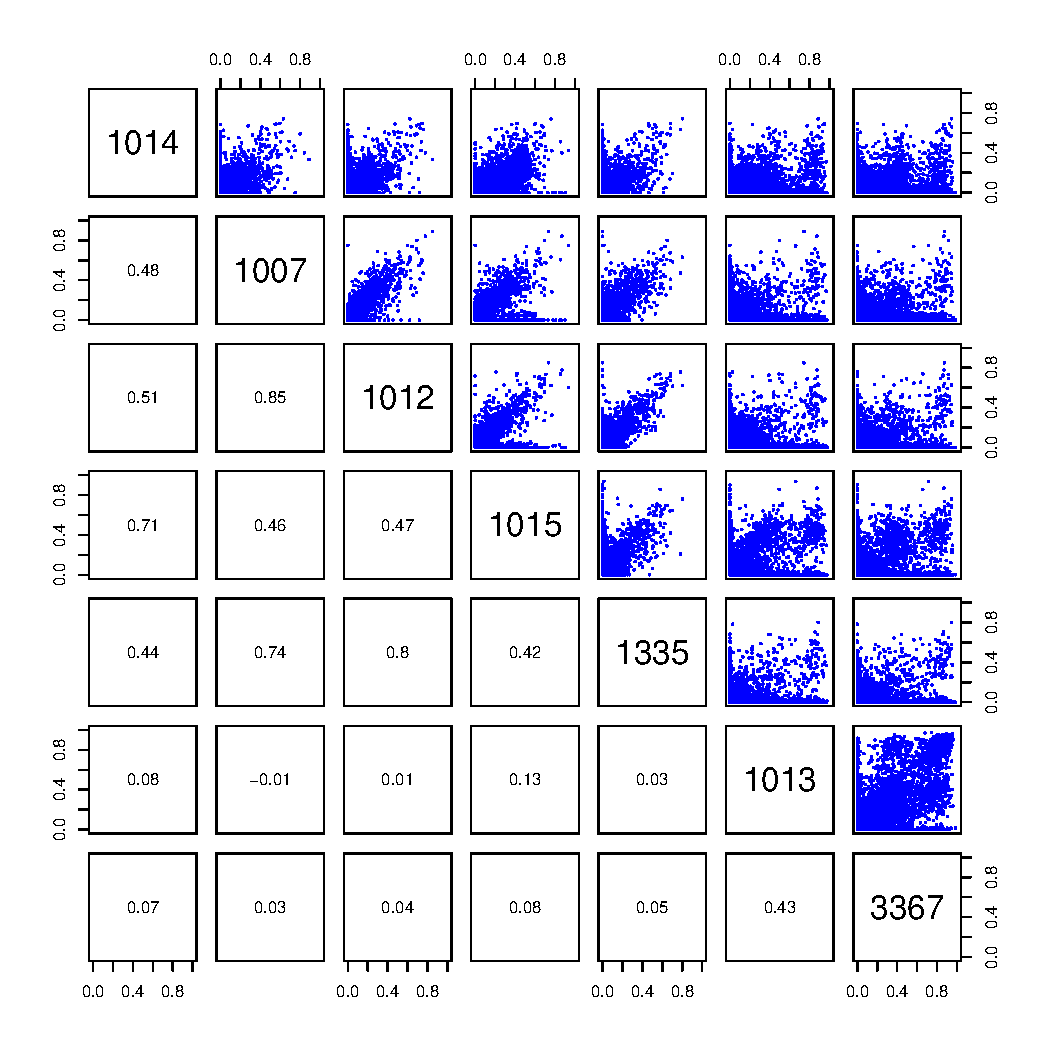
\includegraphics[width=\maxwidth]{figs-knitr/unnamed-chunk-38-1} 

}



\end{knitrout}


Another big NY chunk.  VA: undel, snpy; AU: maybe del, snpy; Wales: undel, snpy (but maybe low nonref);
 Gyre: maybe del, few snps; 1015: del, few snps; IT: undel, snpy (but low); NY del, few snps.
 I.e., NY, 1015 are hemi; gyre is homo-ref, others seem het.
\begin{knitrout}\footnotesize
\definecolor{shadecolor}{rgb}{0.969, 0.969, 0.969}\color{fgcolor}\begin{kframe}
\begin{alltt}
\hlkwd{hemi.chunk}\hlstd{(}\hlkwd{c}\hlstd{(}\hlstr{'Chr6:174501'}\hlstd{,}\hlstr{'Chr6:346501'}\hlstd{),} \hlkwc{margin}\hlstd{=}\hlnum{10000}\hlstd{)}
\end{alltt}
\begin{verbatim}
# Rows 576 : 583 
#              chr  start    end length tp1007 tp1012 tp1013 tp1014 tp1015 IT tp1335 pattern
# Chr6:174401 Chr6 174401 174500    100     NA     NA  0.592     NA     NA NA     NA      20
# Chr6:174501 Chr6 174501 176600   2100     NA  0.589  0.592  0.709  0.611 NA  0.582      75
# Chr6:176601 Chr6 176601 181700   5100     NA     NA  0.592  0.709  0.611 NA  0.582      35
# Chr6:181701 Chr6 181701 268500  86800     NA     NA     NA  0.709  0.611 NA  0.582      15
# Chr6:268501 Chr6 268501 272600   4100     NA     NA     NA     NA     NA NA     NA      00
# Chr6:272601 Chr6 272601 272900    300     NA     NA     NA     NA  0.586 NA  0.589      05
# Chr6:272901 Chr6 272901 346300  73400     NA     NA     NA  0.685  0.586 NA  0.589      15
# Chr6:346301 Chr6 346301 346500    200     NA     NA     NA  0.685     NA NA  0.589      11
# Chr6:346501 Chr6 346501 347000    500     NA     NA     NA  0.685     NA NA     NA      10
# Chr6:347001 Chr6 347001 660300 313300     NA     NA     NA     NA     NA NA     NA      00
\end{verbatim}
\end{kframe}

{\centering 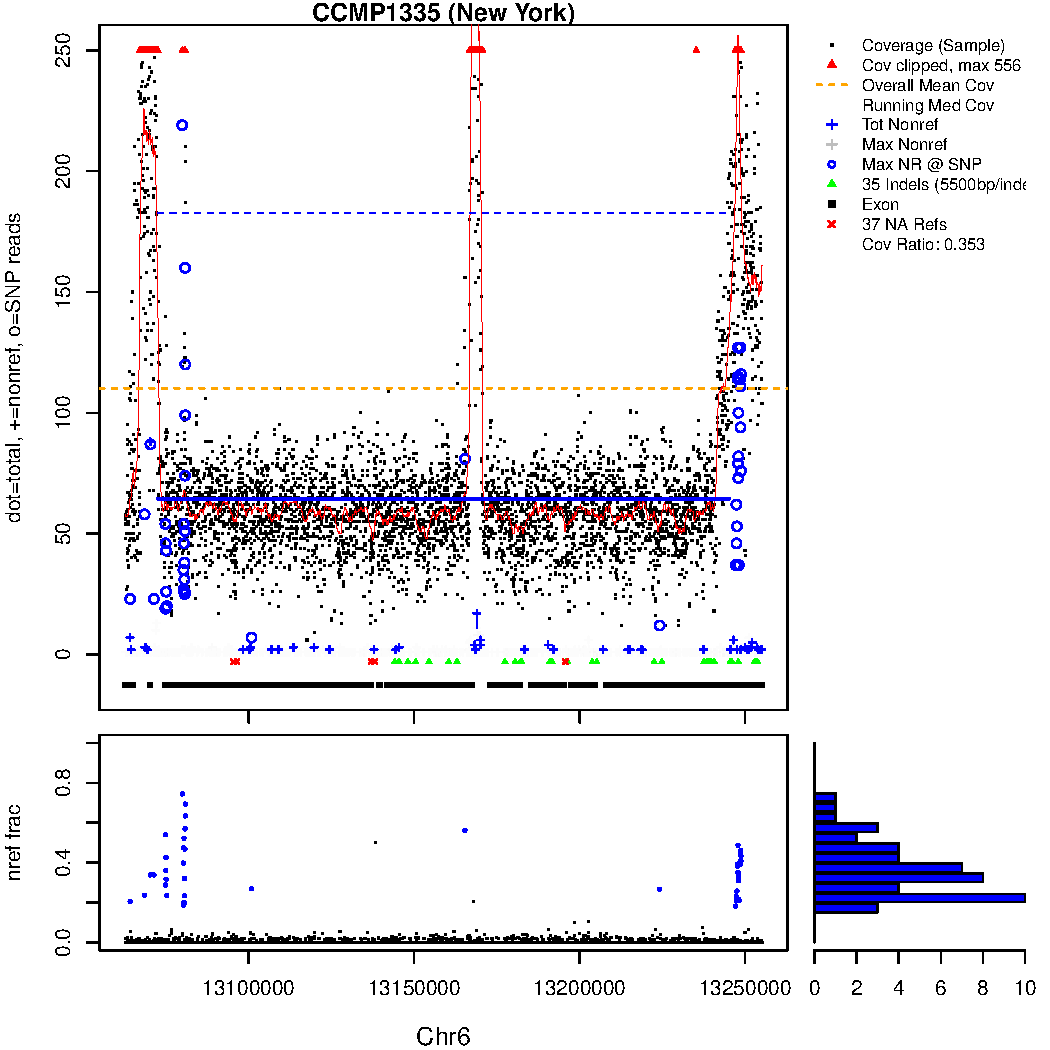
\includegraphics[width=\maxwidth]{figs-knitr/unnamed-chunk-39-1} 
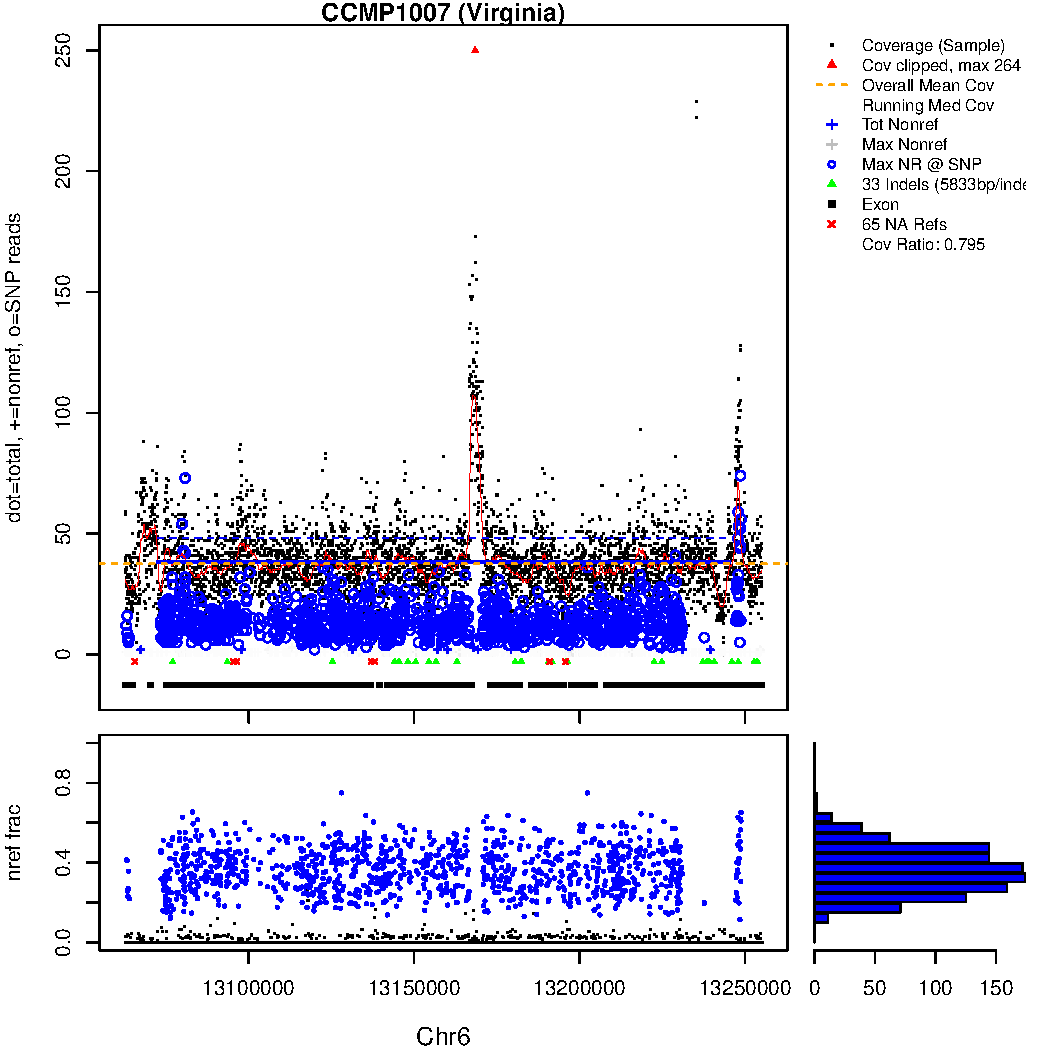
\includegraphics[width=\maxwidth]{figs-knitr/unnamed-chunk-39-2} 
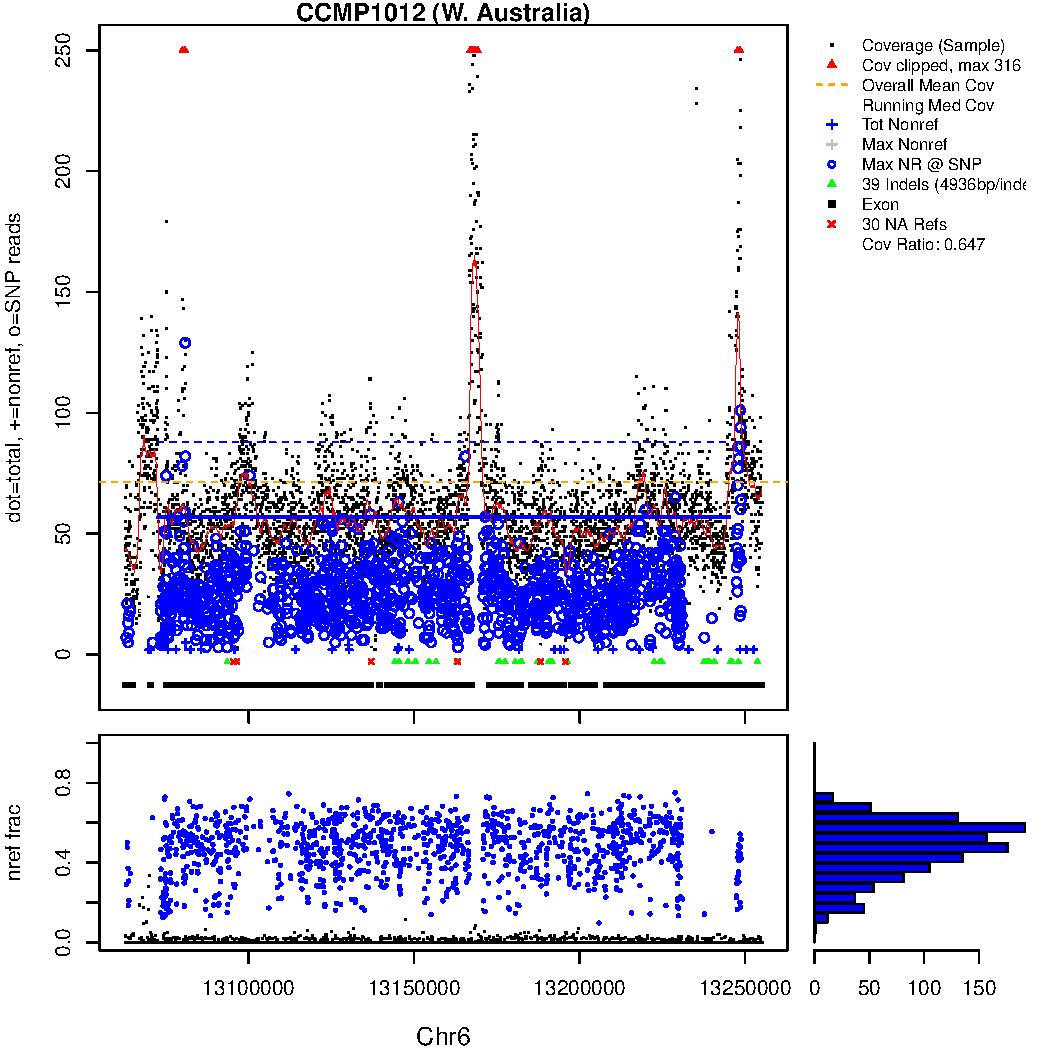
\includegraphics[width=\maxwidth]{figs-knitr/unnamed-chunk-39-3} 
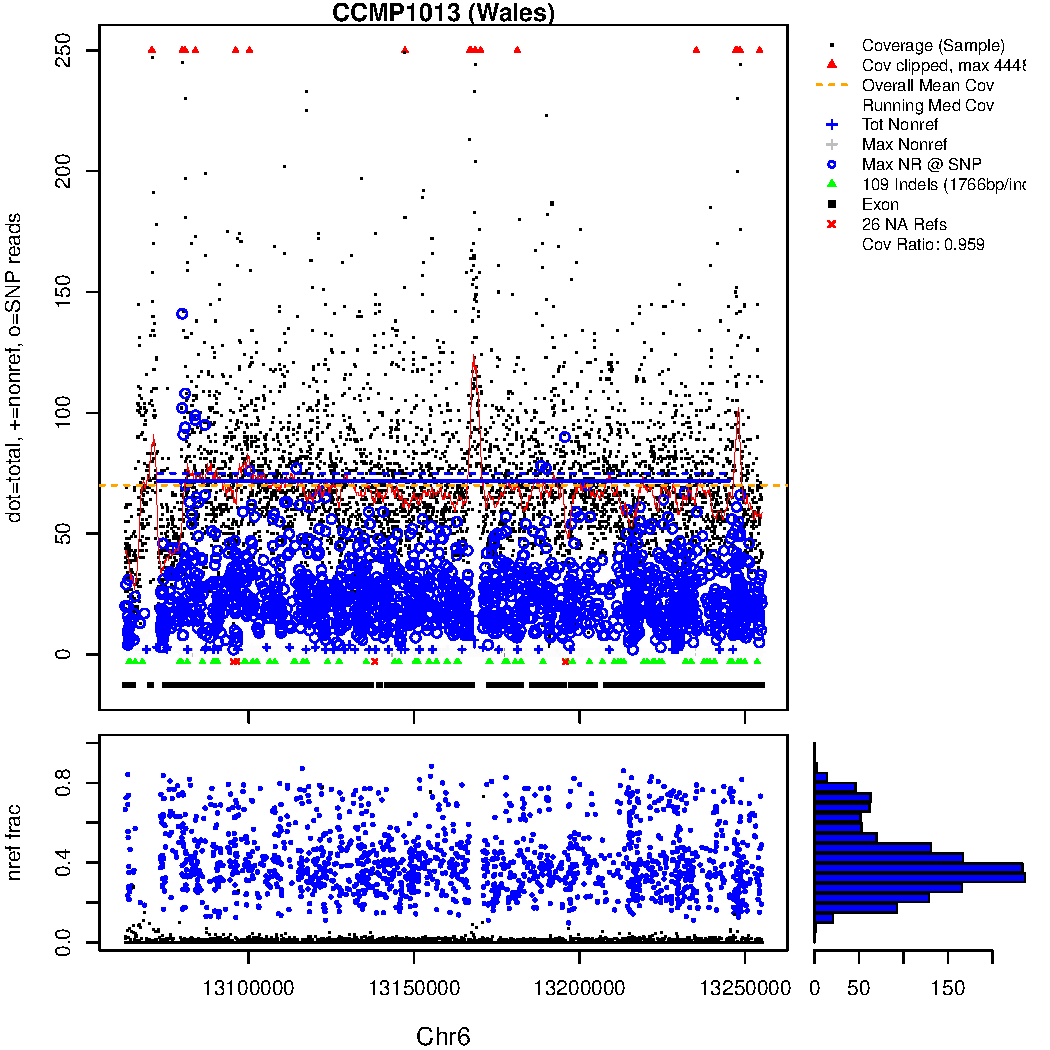
\includegraphics[width=\maxwidth]{figs-knitr/unnamed-chunk-39-4} 
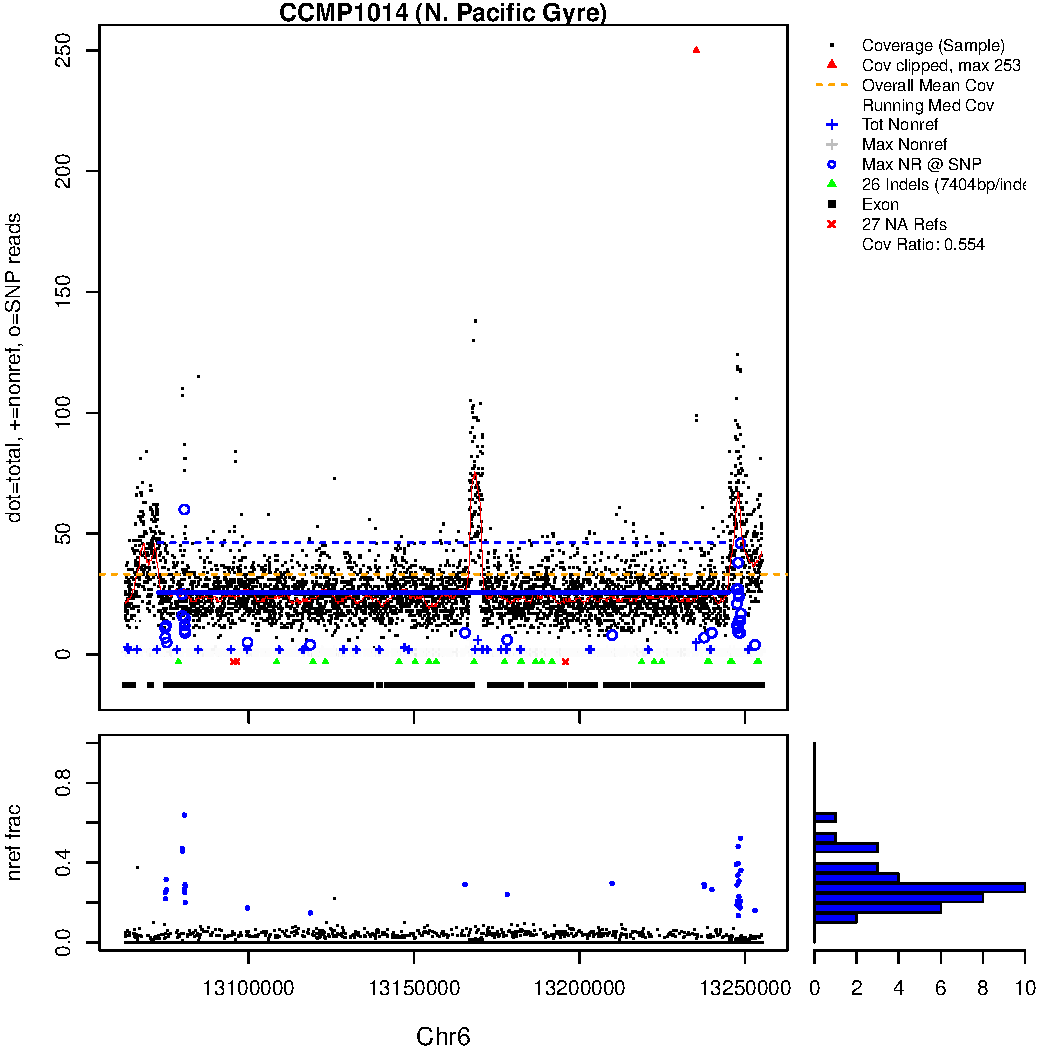
\includegraphics[width=\maxwidth]{figs-knitr/unnamed-chunk-39-5} 
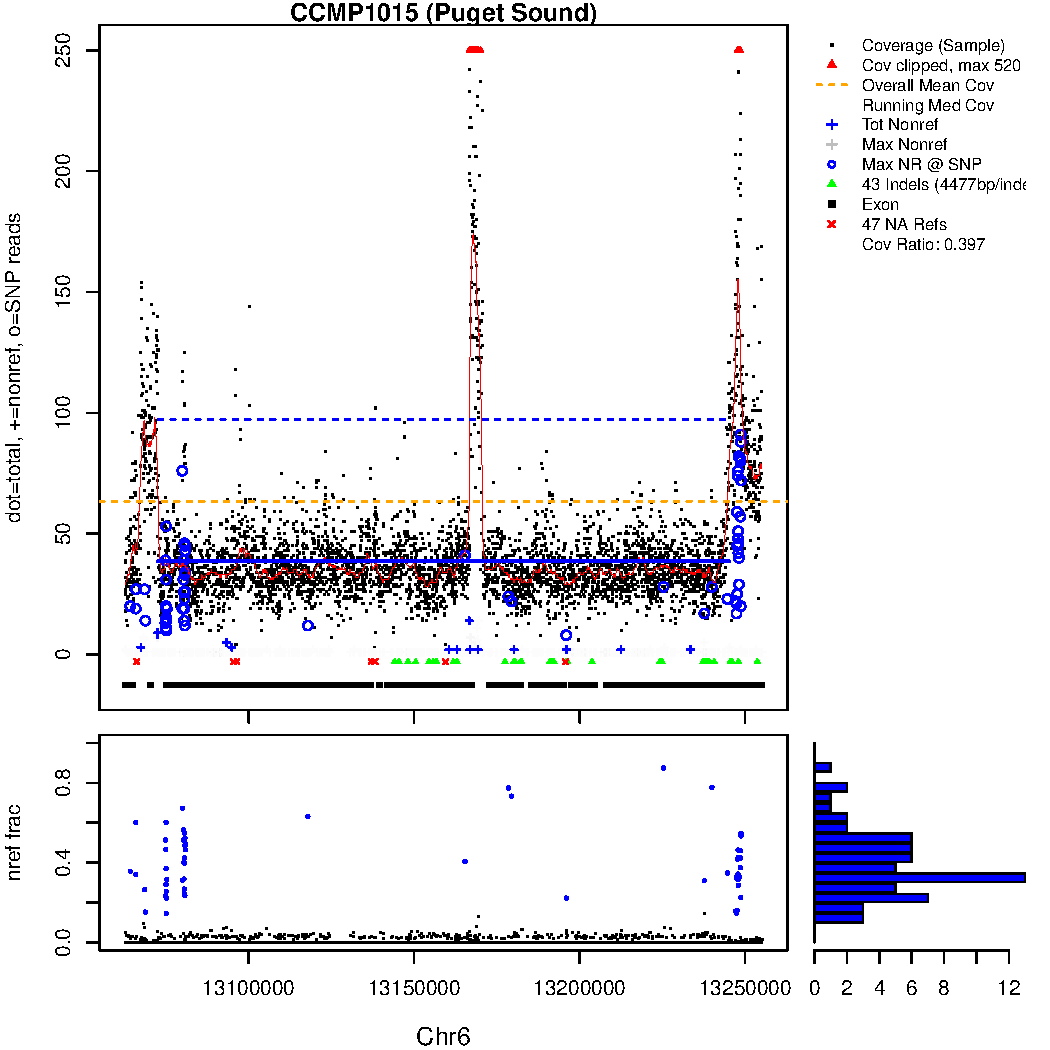
\includegraphics[width=\maxwidth]{figs-knitr/unnamed-chunk-39-6} 
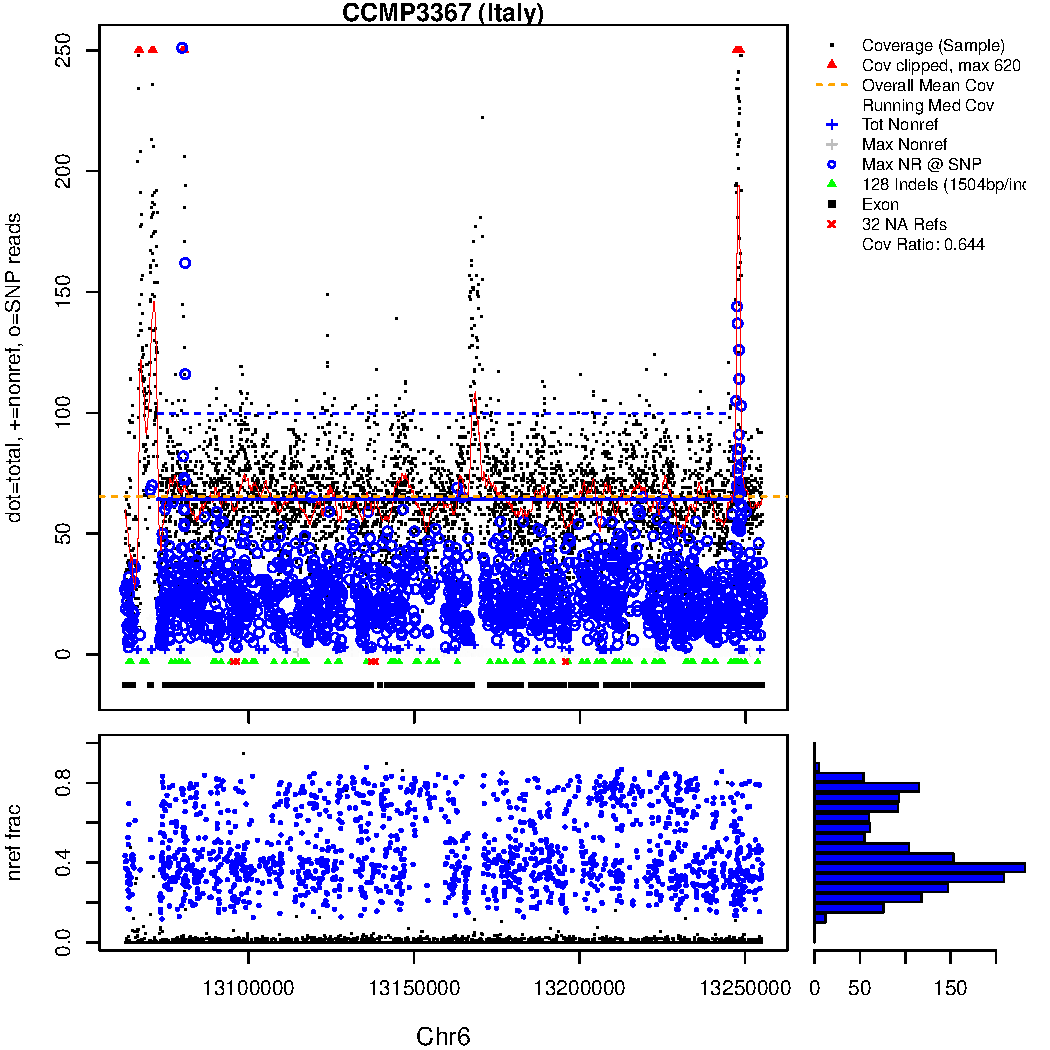
\includegraphics[width=\maxwidth]{figs-knitr/unnamed-chunk-39-7} 

}



\end{knitrout}

Are IT/Wales low nonref?  not really:

\begin{knitrout}\footnotesize
\definecolor{shadecolor}{rgb}{0.969, 0.969, 0.969}\color{fgcolor}\begin{kframe}
\begin{alltt}
\hlkwd{show.allele.scatter}\hlstd{(}\hlnum{3}\hlstd{,}\hlkwd{seg.mask}\hlstd{(}\hlkwd{chrloc2g}\hlstd{(}\hlstr{'Chr6:174501'}\hlstd{),}\hlkwd{chrloc2g}\hlstd{(}\hlstr{'Chr6:346501'}\hlstd{)))}
\end{alltt}
\begin{verbatim}
#      [,1]   [,2]   [,3]   [,4]    [,5]  [,6]    [,7]    [,8]     [,9]     [,10]    [,11] 
# [1,] "blue" "nm3"  "nm3x" "nm3hi" "red" "black" "green" "orange" "ornghi" "nzgrey" "grey"
# [2,] "1747" "1236" NA     "0"     NA    NA      NA      NA       NA       NA       NA
\end{verbatim}
\begin{alltt}
\hlkwd{show.allele.scatter}\hlstd{(}\hlnum{6}\hlstd{,}\hlkwd{seg.mask}\hlstd{(}\hlkwd{chrloc2g}\hlstd{(}\hlstr{'Chr6:174501'}\hlstd{),}\hlkwd{chrloc2g}\hlstd{(}\hlstr{'Chr6:346501'}\hlstd{)))}
\end{alltt}
\begin{verbatim}
#      [,1]   [,2]   [,3]   [,4]    [,5]  [,6]    [,7]    [,8]     [,9]     [,10]    [,11] 
# [1,] "blue" "nm3"  "nm3x" "nm3hi" "red" "black" "green" "orange" "ornghi" "nzgrey" "grey"
# [2,] "1803" "1070" NA     "0"     NA    NA      NA      NA       NA       NA       NA
\end{verbatim}
\end{kframe}

{\centering 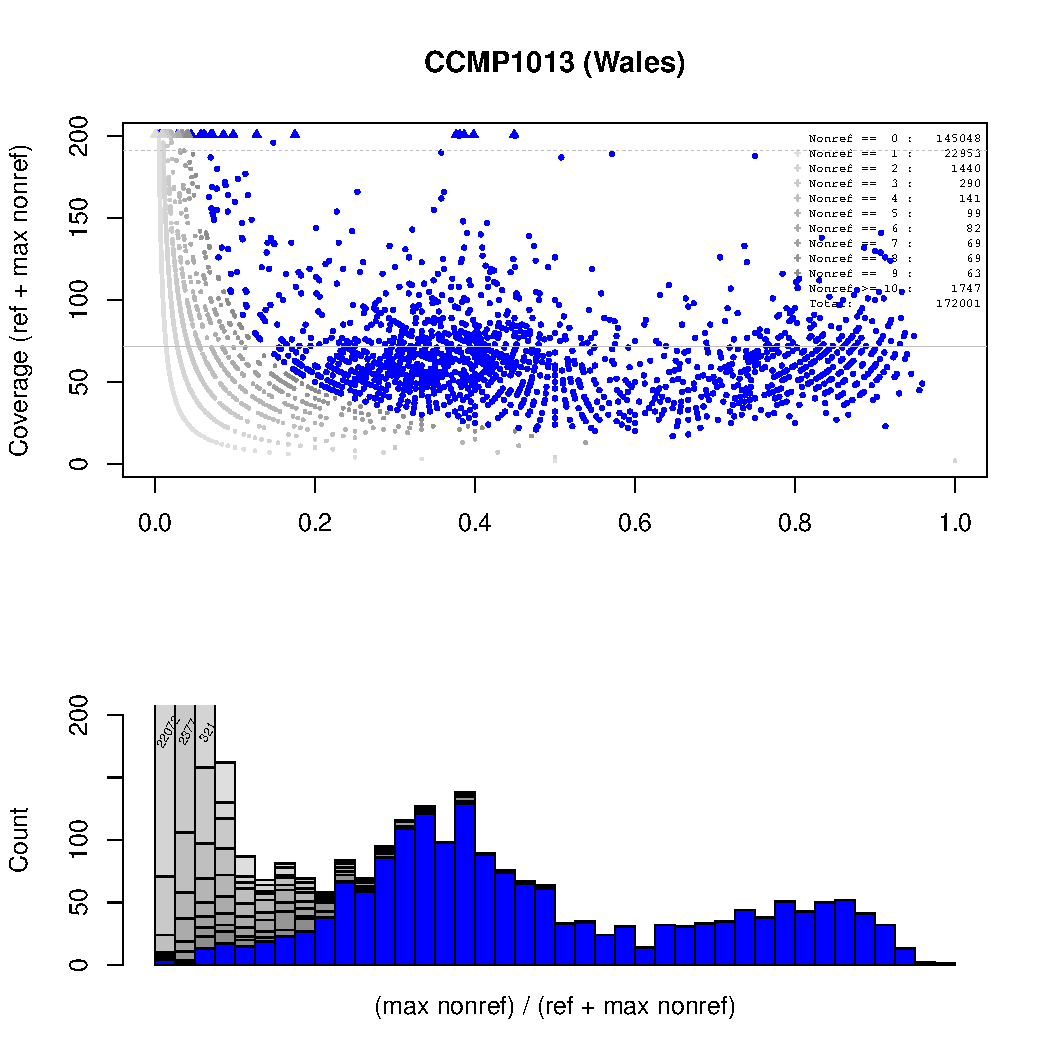
\includegraphics[width=\maxwidth]{figs-knitr/unnamed-chunk-40-1} 
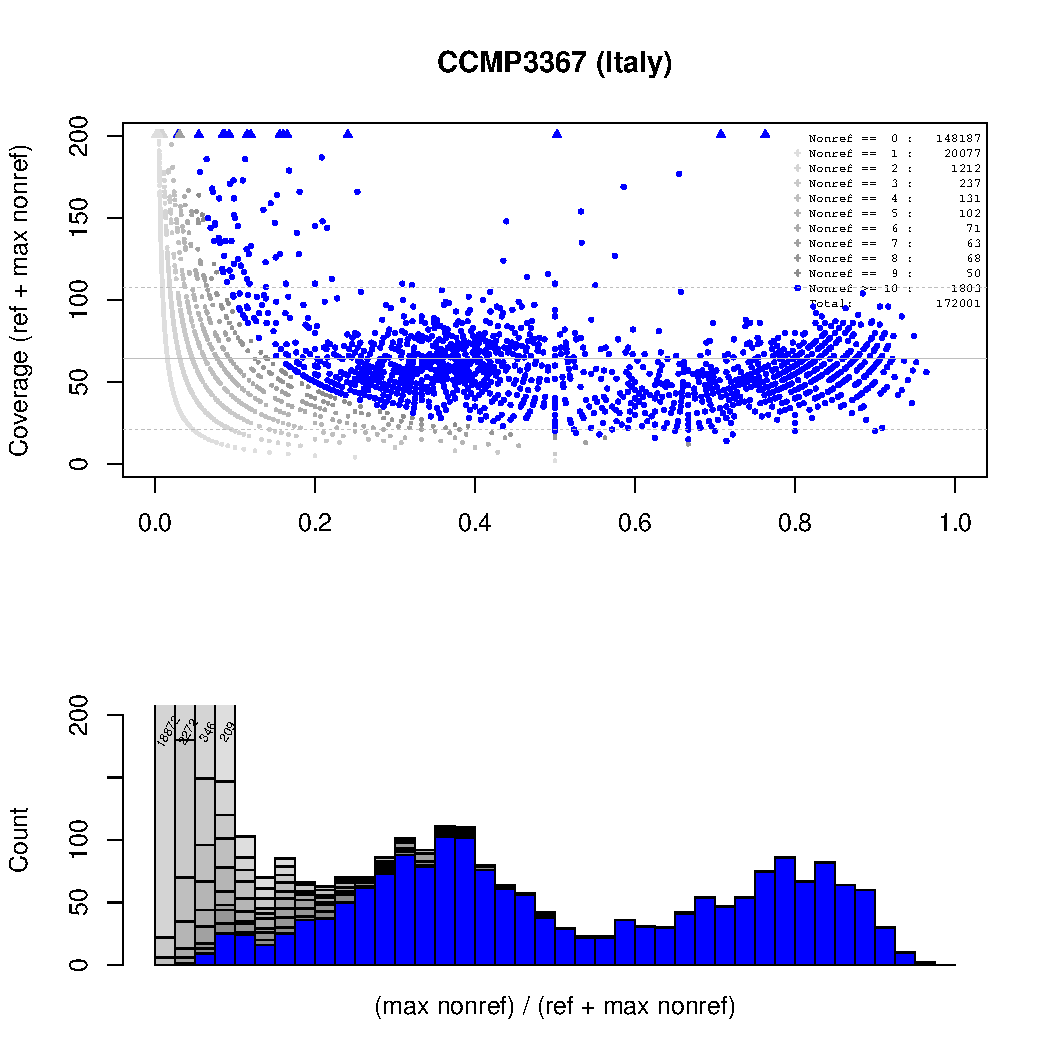
\includegraphics[width=\maxwidth]{figs-knitr/unnamed-chunk-40-2} 

}



\end{knitrout}

Another NY chunk: 1st 96k of chr23.  VA: undel, snpy, except for about 20k.  AUS: ditto, 1015: ditto.
1014: del, snpy except same 20k.
IT/wales: undel, snpy all over.
NY: 96k del, snp-free, followed by 100K @ 1.5x.

Especially interesting: Approx 10k at left tip in 1007+1012 is hemizygous, but nonref frac near 0.7.

\begin{knitrout}\footnotesize
\definecolor{shadecolor}{rgb}{0.969, 0.969, 0.969}\color{fgcolor}\begin{kframe}
\begin{alltt}
\hlkwd{hemi.chunk}\hlstd{(}\hlkwd{c}\hlstd{(}\hlstr{'Chr23:1'}\hlstd{,}\hlstr{'Chr23:96001'}\hlstd{),}\hlkwc{margin}\hlstd{=}\hlnum{10000}\hlstd{)}
\end{alltt}
\begin{verbatim}
# Rows 458 : 461 
#                 chr   start     end length tp1007 tp1012 tp1013 tp1014 tp1015 IT tp1335 pattern
# Chr22:1057565 Chr22 1057565 1057564      0     NA     NA     NA     NA     NA NA     NA     000
# Chr23:1       Chr23       1    8900   8900  0.748  0.739     NA  0.694     NA NA  0.573     151
# Chr23:8901    Chr23    8901    9100    200     NA  0.739     NA  0.694     NA NA  0.573     051
# Chr23:9101    Chr23    9101   96000  86900     NA     NA     NA  0.694     NA NA  0.573     011
# Chr23:96001   Chr23   96001  190200  94200     NA     NA     NA  0.694     NA NA     NA     010
# Chr23:190201  Chr23  190201  305400 115200     NA     NA     NA     NA     NA NA     NA     000
\end{verbatim}
\end{kframe}

{\centering 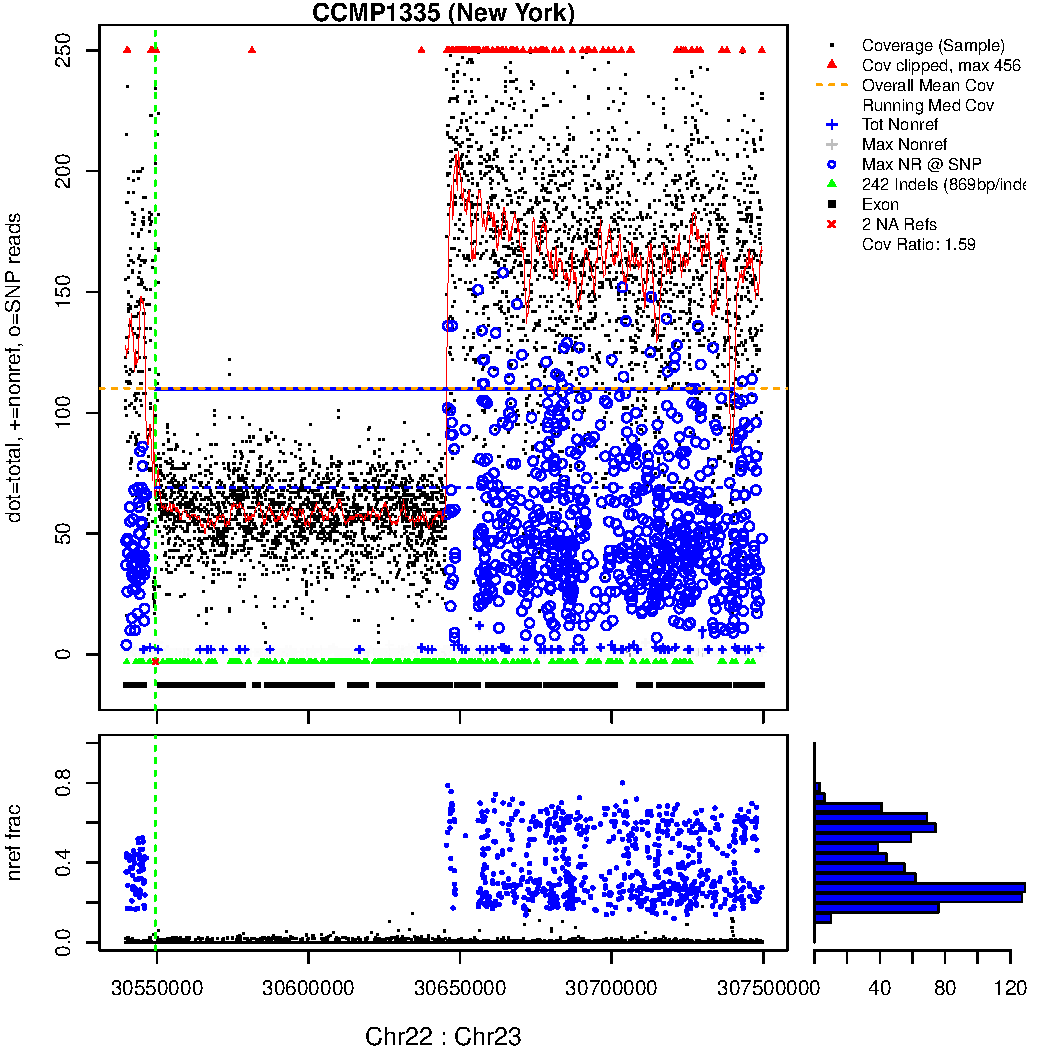
\includegraphics[width=\maxwidth]{figs-knitr/unnamed-chunk-41-1} 
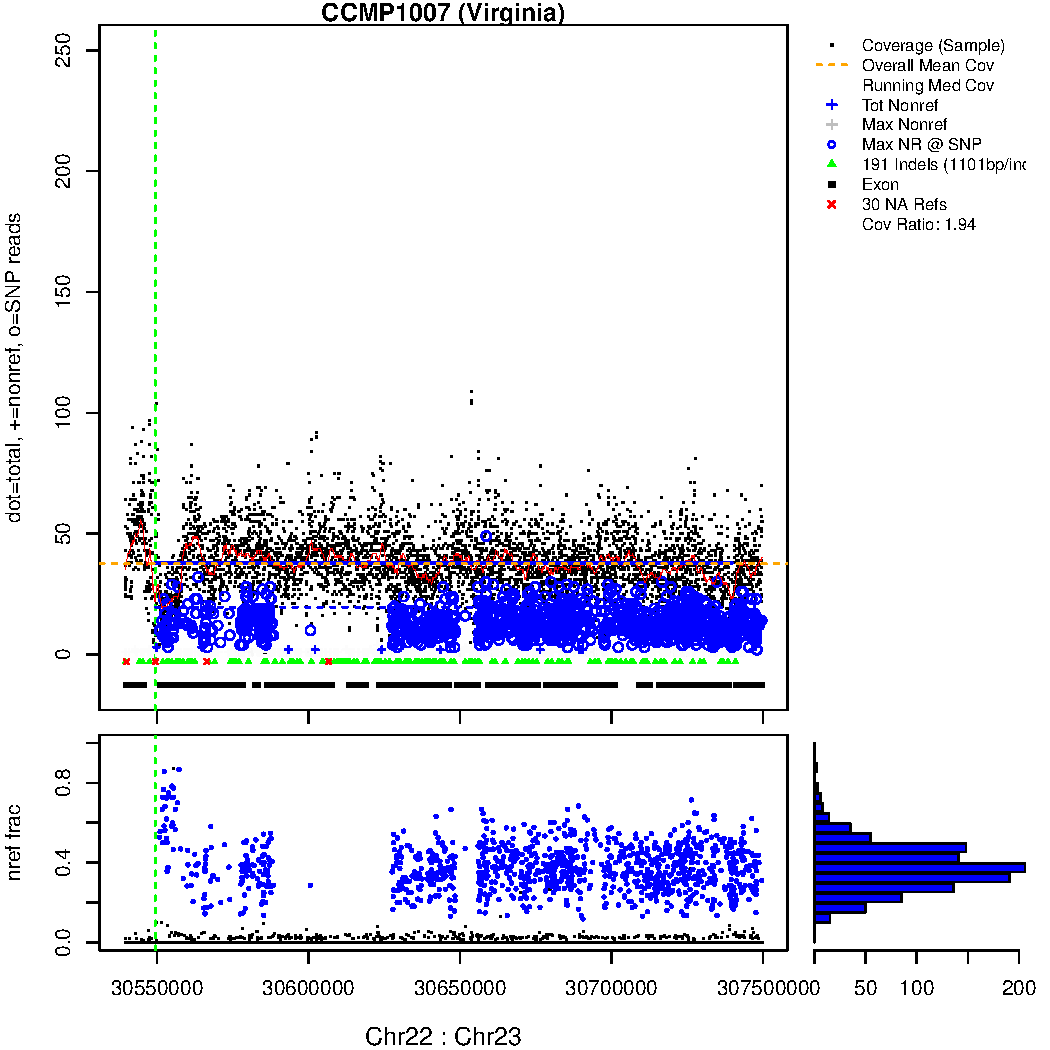
\includegraphics[width=\maxwidth]{figs-knitr/unnamed-chunk-41-2} 
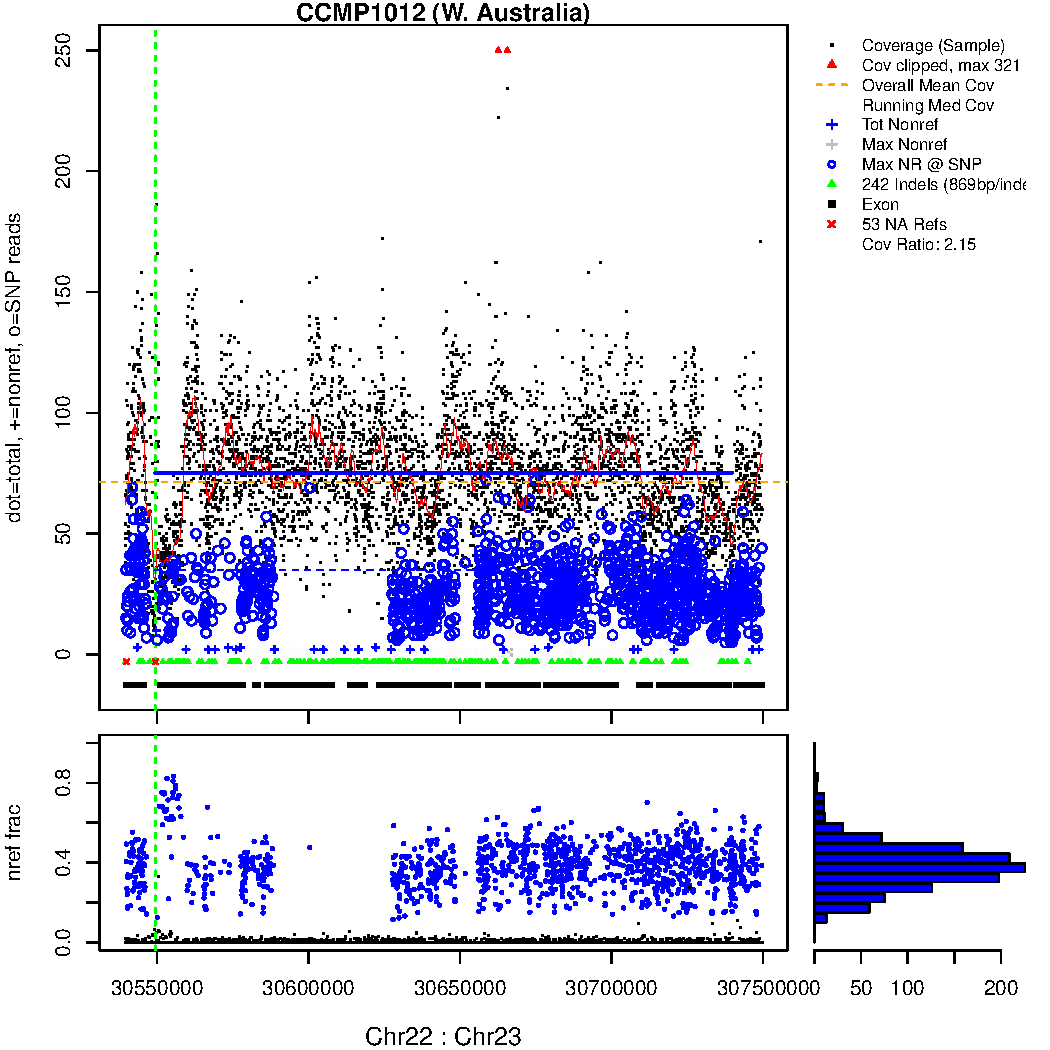
\includegraphics[width=\maxwidth]{figs-knitr/unnamed-chunk-41-3} 
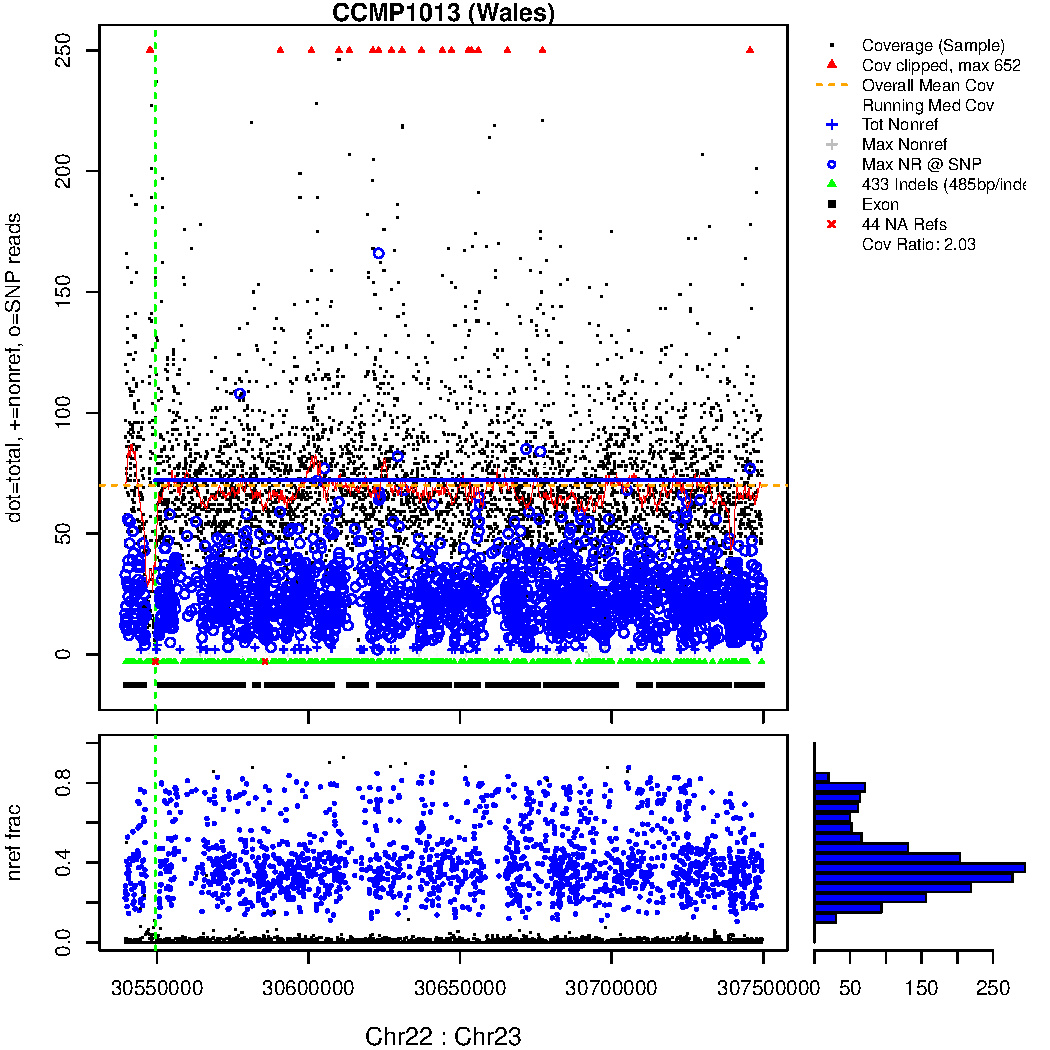
\includegraphics[width=\maxwidth]{figs-knitr/unnamed-chunk-41-4} 
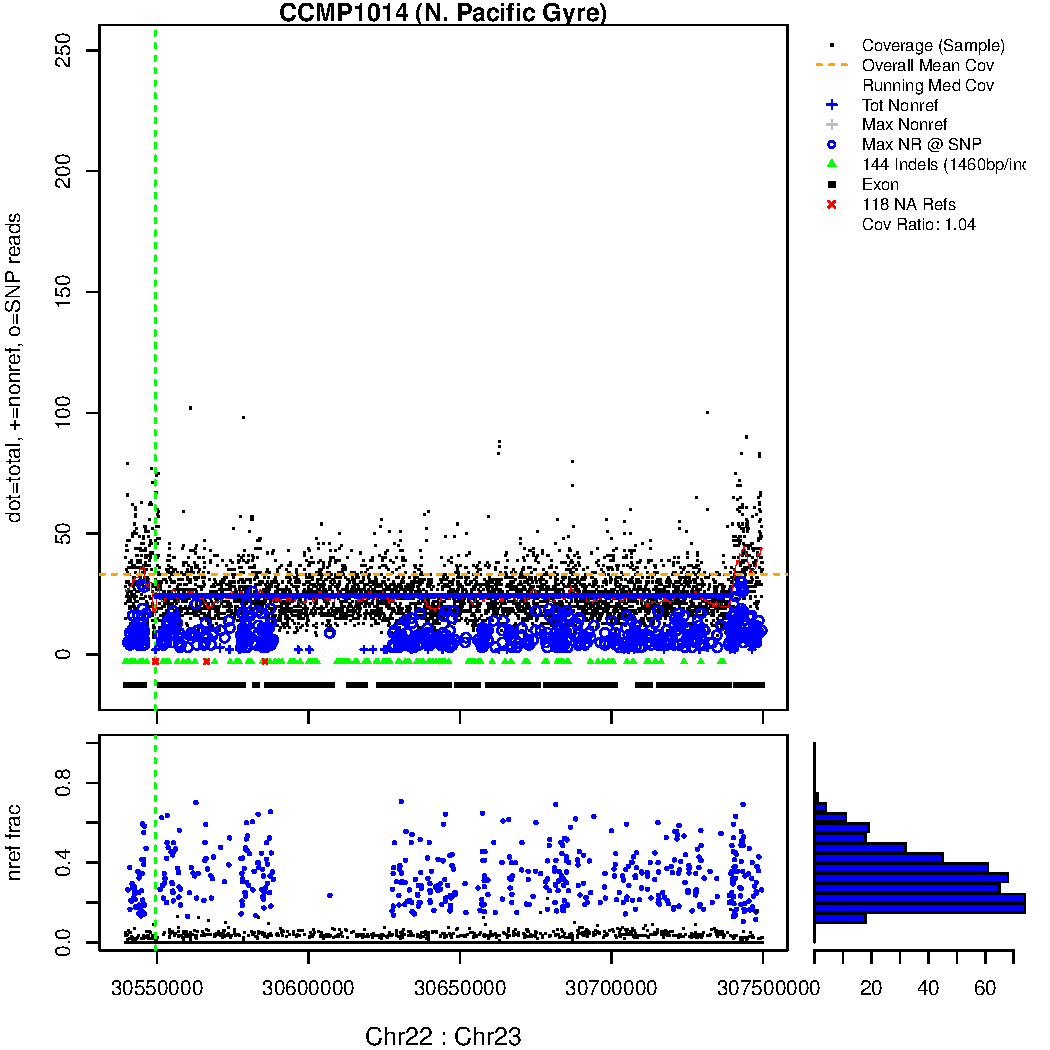
\includegraphics[width=\maxwidth]{figs-knitr/unnamed-chunk-41-5} 
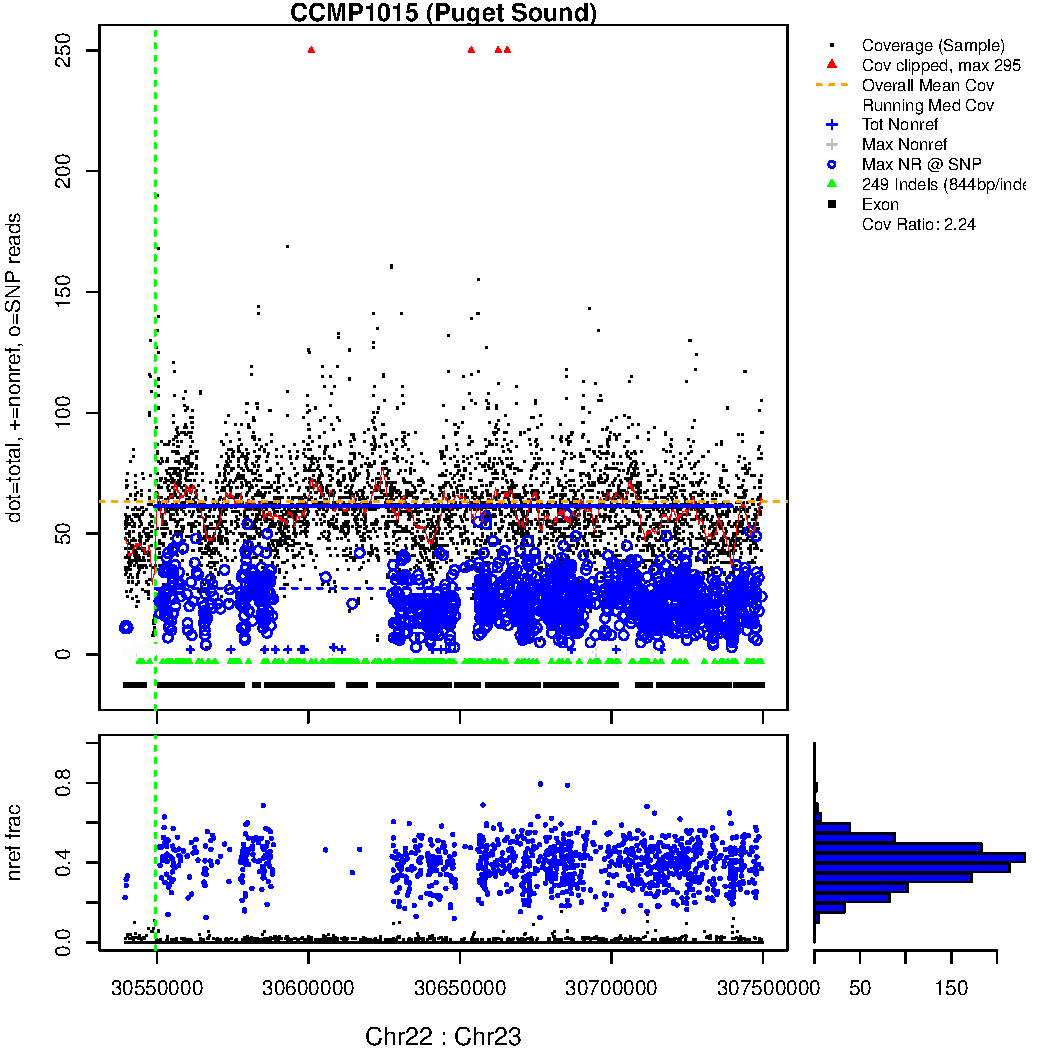
\includegraphics[width=\maxwidth]{figs-knitr/unnamed-chunk-41-6} 
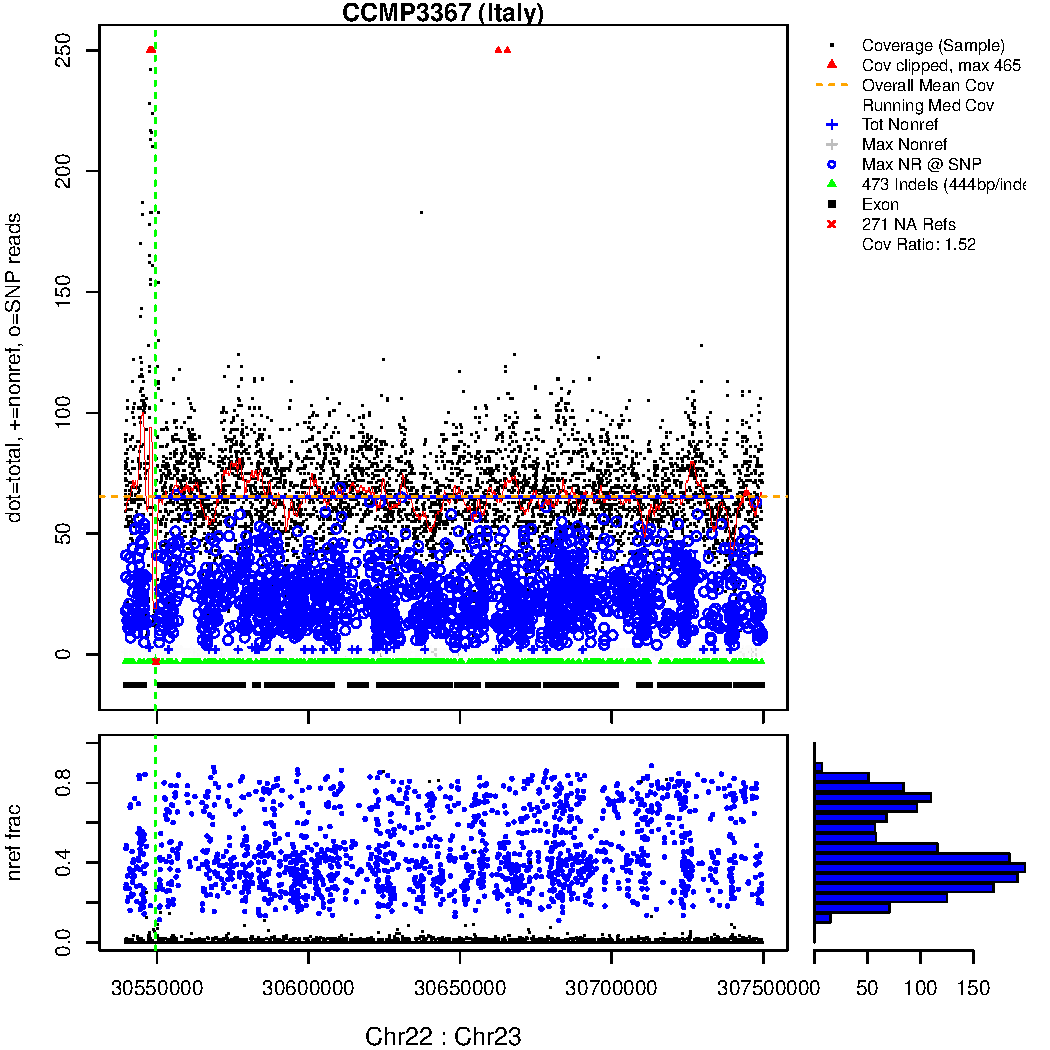
\includegraphics[width=\maxwidth]{figs-knitr/unnamed-chunk-41-7} 

}



\end{knitrout}

Great snap of locality in nonref frac in NY: left 96k of chr23 is hemi, snpless; rest is 1.5x, and snp-frac is bi-modal at about 1/3 , 2/3, \emph{except} for a 50k chunk near the middle, which is only 1/3.
1007,1012, 1015: normal coverage , 50K LOH
1013/IT: normal coverage, snpy, usual bimodal pattern, heavier on 0.4.
Gyre has 200K  region at .7 coverage, with the same 50K LOH.  SNP density is lower than 1015, say  (as usual) , but appears unimodal, despite \emph{elevated} coverage on the other 250K.

\begin{knitrout}\footnotesize
\definecolor{shadecolor}{rgb}{0.969, 0.969, 0.969}\color{fgcolor}\begin{kframe}
\begin{alltt}
\hlkwd{hemi.chunk}\hlstd{(}\hlkwd{c}\hlstd{(}\hlstr{'Chr23:1'}\hlstd{,}\hlstr{'Chr23:454954'}\hlstd{),}\hlnum{7}\hlstd{,}\hlkwc{margin}\hlstd{=}\hlnum{1000}\hlstd{)}
\end{alltt}
\begin{verbatim}
# Rows 458 : 469 
#                 chr   start     end length tp1007 tp1012 tp1013 tp1014 tp1015    IT tp1335 pattern
# Chr22:1057565 Chr22 1057565 1057564      0     NA     NA     NA     NA     NA    NA     NA     000
# Chr23:1       Chr23       1    8900   8900  0.748  0.739     NA  0.694     NA    NA  0.573     151
# Chr23:8901    Chr23    8901    9100    200     NA  0.739     NA  0.694     NA    NA  0.573     051
# Chr23:9101    Chr23    9101   96000  86900     NA     NA     NA  0.694     NA    NA  0.573     011
# Chr23:96001   Chr23   96001  190200  94200     NA     NA     NA  0.694     NA    NA     NA     010
# Chr23:190201  Chr23  190201  305400 115200     NA     NA     NA     NA     NA    NA     NA     000
# Chr23:305401  Chr23  305401  307700   2300     NA     NA     NA     NA     NA 0.737     NA     002
# Chr23:307701  Chr23  307701  341700  34000     NA     NA     NA     NA     NA    NA     NA     000
# Chr23:341701  Chr23  341701  342300    600     NA     NA     NA     NA     NA 0.197     NA     002
# Chr23:342301  Chr23  342301  444400 102100     NA     NA     NA     NA     NA    NA     NA     000
# Chr23:444401  Chr23  444401  447900   3500     NA     NA  0.529     NA     NA    NA     NA     020
# Chr23:447901  Chr23  447901  454953   7053     NA     NA     NA     NA     NA    NA     NA     000
# Chr23:454954  Chr23  454954  454953      0     NA     NA     NA     NA     NA    NA     NA     000
# Chr24:1       Chr24       1   10900  10900     NA     NA     NA     NA     NA    NA     NA     000
\end{verbatim}
\begin{alltt}
\hlkwd{hemi.chunk}\hlstd{(}\hlkwd{c}\hlstd{(}\hlstr{'Chr23:1'}\hlstd{,}\hlstr{'Chr23:454954'}\hlstd{),}\hlnum{1}\hlopt{:}\hlnum{6}\hlstd{,}\hlkwc{margin}\hlstd{=}\hlnum{1000}\hlstd{)}
\end{alltt}
\begin{verbatim}
# Rows 458 : 469 
#                 chr   start     end length tp1007 tp1012 tp1013 tp1014 tp1015    IT tp1335 pattern
# Chr22:1057565 Chr22 1057565 1057564      0     NA     NA     NA     NA     NA    NA     NA     000
# Chr23:1       Chr23       1    8900   8900  0.748  0.739     NA  0.694     NA    NA  0.573     151
# Chr23:8901    Chr23    8901    9100    200     NA  0.739     NA  0.694     NA    NA  0.573     051
# Chr23:9101    Chr23    9101   96000  86900     NA     NA     NA  0.694     NA    NA  0.573     011
# Chr23:96001   Chr23   96001  190200  94200     NA     NA     NA  0.694     NA    NA     NA     010
# Chr23:190201  Chr23  190201  305400 115200     NA     NA     NA     NA     NA    NA     NA     000
# Chr23:305401  Chr23  305401  307700   2300     NA     NA     NA     NA     NA 0.737     NA     002
# Chr23:307701  Chr23  307701  341700  34000     NA     NA     NA     NA     NA    NA     NA     000
# Chr23:341701  Chr23  341701  342300    600     NA     NA     NA     NA     NA 0.197     NA     002
# Chr23:342301  Chr23  342301  444400 102100     NA     NA     NA     NA     NA    NA     NA     000
# Chr23:444401  Chr23  444401  447900   3500     NA     NA  0.529     NA     NA    NA     NA     020
# Chr23:447901  Chr23  447901  454953   7053     NA     NA     NA     NA     NA    NA     NA     000
# Chr23:454954  Chr23  454954  454953      0     NA     NA     NA     NA     NA    NA     NA     000
# Chr24:1       Chr24       1   10900  10900     NA     NA     NA     NA     NA    NA     NA     000
\end{verbatim}
\end{kframe}

{\centering 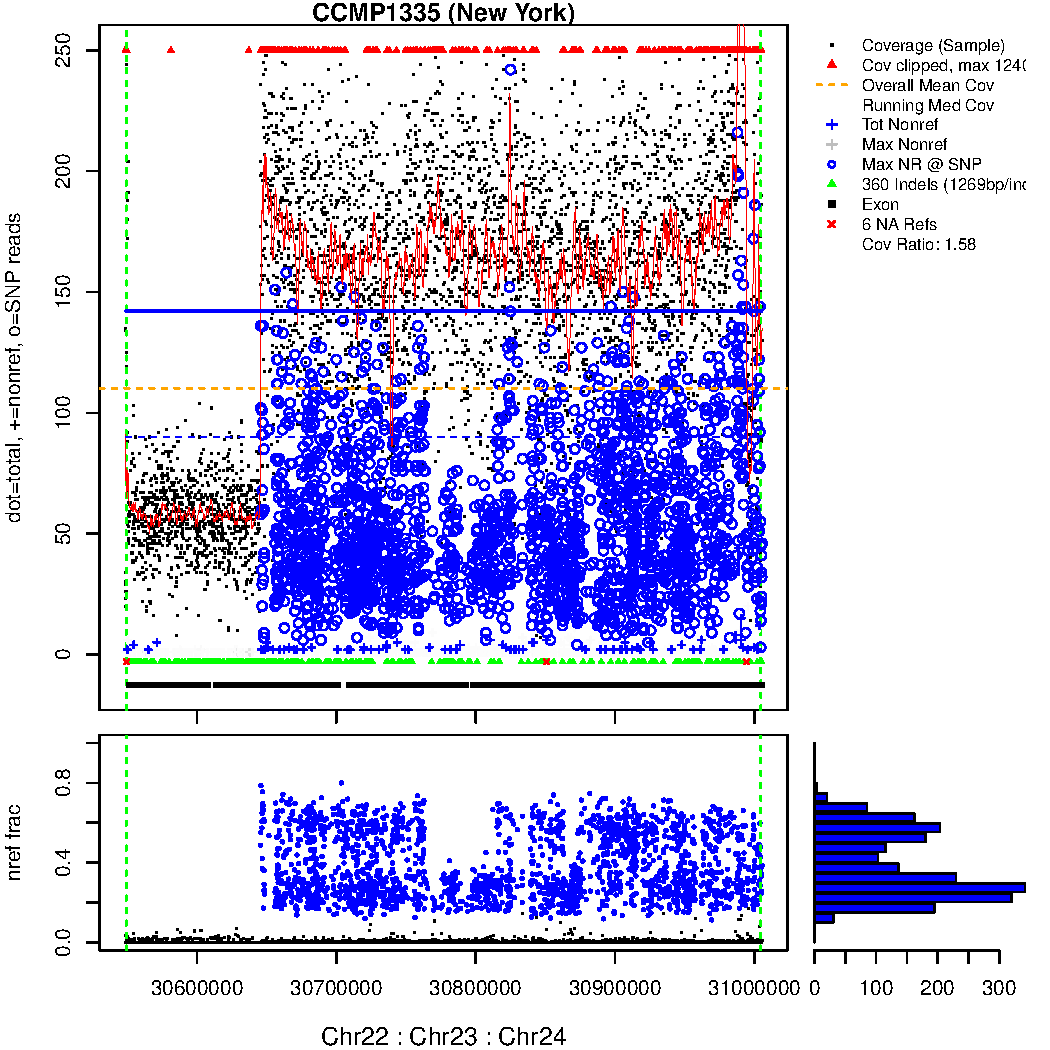
\includegraphics[width=\maxwidth]{figs-knitr/unnamed-chunk-42-1} 
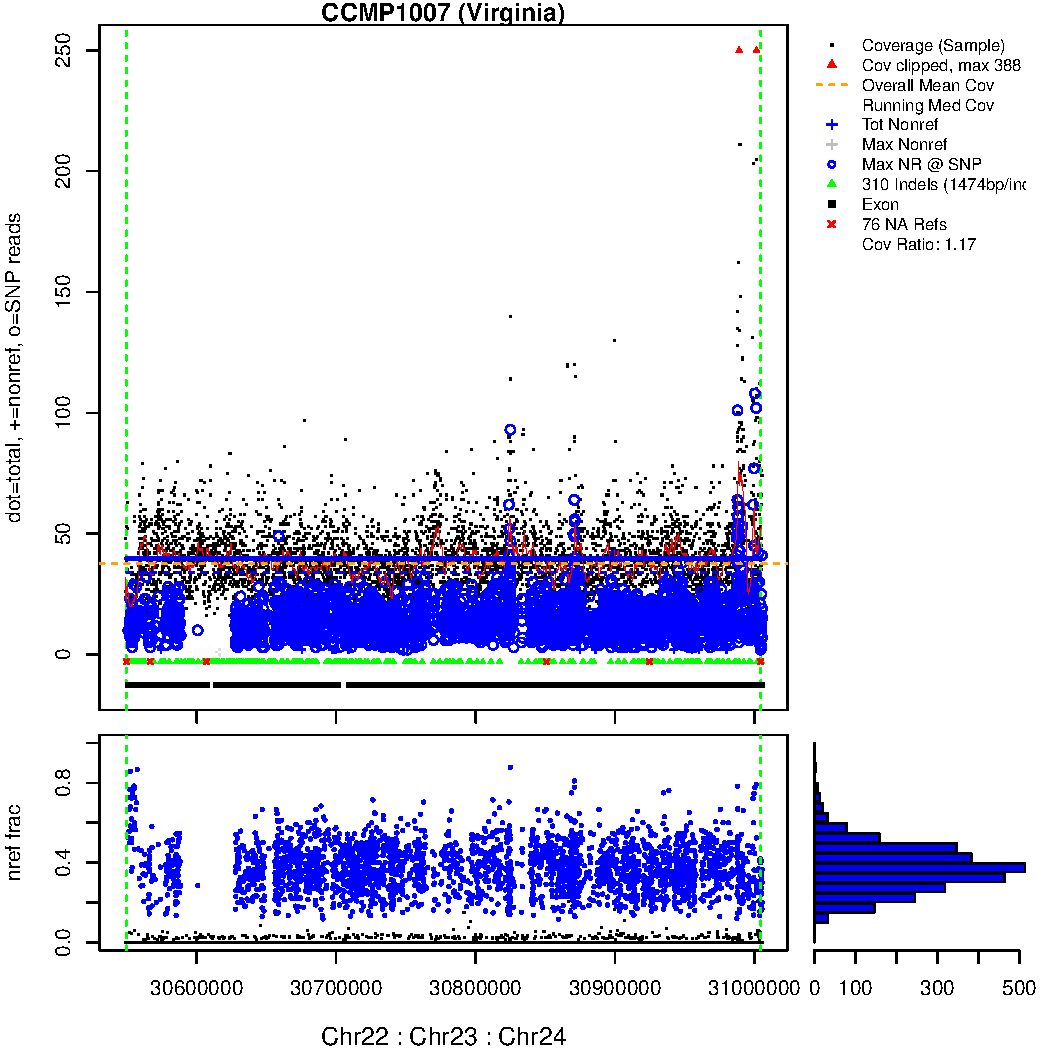
\includegraphics[width=\maxwidth]{figs-knitr/unnamed-chunk-42-2} 
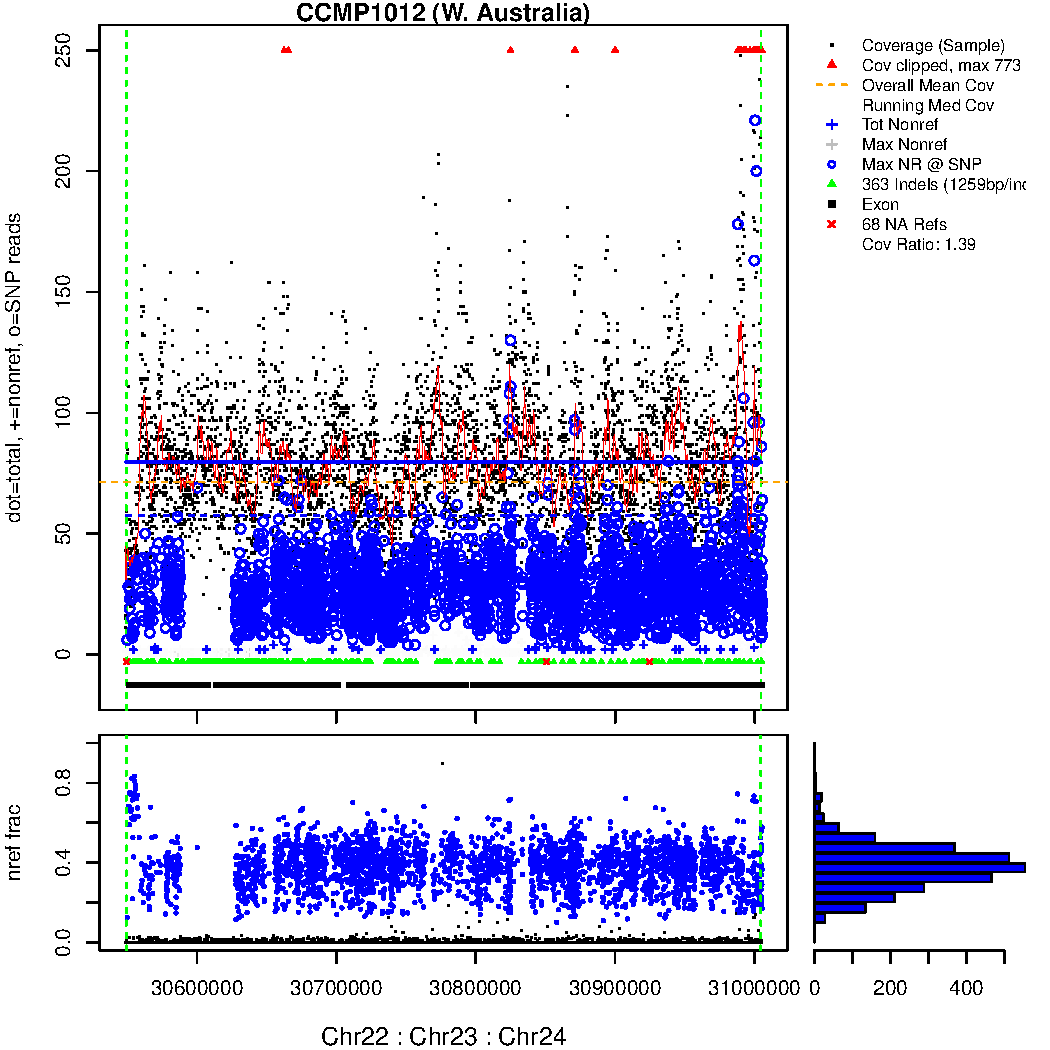
\includegraphics[width=\maxwidth]{figs-knitr/unnamed-chunk-42-3} 
\includegraphics[width=\maxwidth]{figs-knitr/unnamed-chunk-42-4} 
\includegraphics[width=\maxwidth]{figs-knitr/unnamed-chunk-42-5} 
\includegraphics[width=\maxwidth]{figs-knitr/unnamed-chunk-42-6} 
\includegraphics[width=\maxwidth]{figs-knitr/unnamed-chunk-42-7} 

}



\end{knitrout}

Other possible trisomies?  23 segments longer than 100k:

\begin{knitrout}\footnotesize
\definecolor{shadecolor}{rgb}{0.969, 0.969, 0.969}\color{fgcolor}\begin{kframe}
\begin{alltt}
\hlstd{trisome} \hlkwb{<-} \hlnum{1.3} \hlopt{<=} \hlstd{cnv}\hlopt{$}\hlstd{cov_ratio} \hlopt{&} \hlstd{cnv}\hlopt{$}\hlstd{cov_ratio} \hlopt{<=} \hlnum{1.7}
\hlkwd{sum}\hlstd{(trisome)}  \hlcom{## [1] 655}
\end{alltt}
\begin{verbatim}
# [1] 655
\end{verbatim}
\begin{alltt}
\hlstd{tripi} \hlkwb{<-} \hlkwd{order}\hlstd{(cnv}\hlopt{$}\hlstd{length[trisome],} \hlkwc{decreasing}\hlstd{=T)}
\hlstd{cnv[trisome,][tripi[}\hlnum{1}\hlopt{:}\hlnum{25}\hlstd{],]}
\end{alltt}
\begin{verbatim}
#      strain       chr   start     end length filtered     type cov_ratio  dup_frac
# 2238 tp1335     Chr14   57701  566500 508800    FALSE CNVnator   1.52069 0.0295811
# 874  tp1014     Chr10  260101  602100 342000    FALSE CNVnator   1.46552 0.0288144
# 1473 tp1015      Chr8  967701 1267200 299500    FALSE CNVnator   1.56302 0.0838569
# 861  tp1014      Chr8  947001 1242800 295800    FALSE CNVnator   1.69376 0.0498832
# 2162 tp1335      Chr6  346501  615100 268600    FALSE CNVnator   1.48366 0.0116308
# 1444 tp1015      Chr6  346301  610700 264400    FALSE CNVnator   1.47470 0.0148579
# 2239 tp1335     Chr14  566701  829300 262600    FALSE CNVnator   1.51717 0.0154430
# 2186 tp1335      Chr8 1005101 1267200 262100    FALSE CNVnator   1.60923 0.0968873
# 873  tp1014     Chr10   28501  246900 218400    FALSE CNVnator   1.57852 0.1519620
# 668  tp1013     Chr18  309801  518300 208500    FALSE CNVnator   1.52974 0.0244539
# 960  tp1014 Chr19c_29    4901  180800 175900     TRUE CNVnator   1.51288 0.0792422
# 2311 tp1335     Chr23   96001  271800 175800    FALSE CNVnator   1.61818 0.0813743
# 2312 tp1335     Chr23  272001  445100 173100    FALSE CNVnator   1.64695 0.0570672
# 945  tp1014     Chr18  374401  547300 172900    FALSE CNVnator   1.38503 0.0378534
# 669  tp1013     Chr18  519801  674100 154300    FALSE CNVnator   1.53579 0.0275490
# 958  tp1014 Chr19b_31       1  151700 151700    FALSE CNVnator   1.40821 0.0380134
# 1273 tp1007     Chr20  263301  408900 145600    FALSE CNVnator   1.69331 0.1602950
# 877  tp1014     Chr10  681001  810000 129000    FALSE CNVnator   1.41920 0.0501984
# 941  tp1014     Chr18    5701  133700 128000    FALSE CNVnator   1.63863 0.0535742
# 1214 tp1007     Chr14   57601  182600 125000    FALSE CNVnator   1.68366 0.0961556
# 986  tp1014     Chr23  332901  455000 122100    FALSE CNVnator   1.65306 0.1235470
# 1223 tp1007     Chr15   86201  197400 111200    FALSE CNVnator   1.54600 0.0547763
# 944  tp1014     Chr18  256801  366300 109500    FALSE CNVnator   1.47736 0.0533481
# 807  tp1014      Chr3       1   98300  98300    FALSE CNVnator   1.33840 0.1953450
# 991  tp1014     Chr24  200101  297400  97300    FALSE CNVnator   1.63994 0.2968230
\end{verbatim}
\end{kframe}
\end{knitrout}

\begin{knitrout}\footnotesize
\definecolor{shadecolor}{rgb}{0.969, 0.969, 0.969}\color{fgcolor}\begin{kframe}
\begin{alltt}
\hlcom{#hemi.chunk(c('Chr14:1','Chr14:829301'),7,margin=1000)}
\hlkwd{hemi.chunk}\hlstd{(}\hlkwd{c}\hlstd{(}\hlstr{'Chr14:1'}\hlstd{,}\hlstr{'Chr14:900701'}\hlstd{),}\hlnum{7}\hlstd{,}\hlkwc{margin}\hlstd{=}\hlnum{1000}\hlstd{)}
\end{alltt}
\begin{verbatim}
# Rows 145 : 150 
#                 chr   start     end length tp1007 tp1012 tp1013 tp1014 tp1015   IT tp1335 pattern
# Chr13:1052196 Chr13 1052196 1052195      0     NA     NA     NA     NA     NA   NA     NA     000
# Chr14:1       Chr14       1  640400 640400     NA     NA     NA     NA     NA   NA     NA     000
# Chr14:640401  Chr14  640401  640600    200  0.609     NA     NA     NA     NA   NA     NA     100
# Chr14:640601  Chr14  640601  773600 133000  0.609  0.607     NA     NA     NA   NA     NA     140
# Chr14:773601  Chr14  773601  777000   3400  0.609     NA     NA     NA     NA   NA     NA     100
# Chr14:777001  Chr14  777001  900700 123700  0.609  0.596     NA     NA     NA   NA     NA     140
# Chr14:900701  Chr14  900701  902400   1700  0.609  0.596     NA     NA     NA 0.59     NA     142
# Chr14:902401  Chr14  902401  918000  15600  0.609  0.596     NA     NA     NA   NA     NA     140
\end{verbatim}
\end{kframe}

{\centering \includegraphics[width=\maxwidth]{figs-knitr/unnamed-chunk-44-1} 

}



\end{knitrout}

cluster of indels in left 300k above seems odd; is it?:

\begin{knitrout}\footnotesize
\definecolor{shadecolor}{rgb}{0.969, 0.969, 0.969}\color{fgcolor}\begin{kframe}
\begin{alltt}
\hlstd{indel.counts} \hlkwb{<-} \hlkwd{unlist}\hlstd{(}\hlkwd{lapply}\hlstd{(full,}\hlkwa{function}\hlstd{(}\hlkwc{x}\hlstd{)\{}\hlkwd{sum}\hlstd{(x}\hlopt{$}\hlstd{indel)\})); indel.counts}
\end{alltt}
\begin{verbatim}
#  1007  1012  1013  1014  1015  3367  1335 
#  7186  8160 15149  5700  8363 15728  7633
\end{verbatim}
\begin{alltt}
\hlkwd{sum}\hlstd{(full[[}\hlnum{7}\hlstd{]]}\hlopt{$}\hlstd{indel[}\hlkwd{chrloc2g}\hlstd{(}\hlstr{'Chr14:1'}\hlstd{)}\hlopt{+}\hlstd{(}\hlnum{1}\hlopt{:}\hlnum{3e5}\hlstd{)])}
\end{alltt}
\begin{verbatim}
# [1] 101
\end{verbatim}
\begin{alltt}
\hlstd{indel.counts[}\hlnum{7}\hlstd{]}\hlopt{/}\hlkwd{nrow}\hlstd{(full[[}\hlnum{7}\hlstd{]])} \hlopt{*} \hlnum{3e5}
\end{alltt}
\begin{verbatim}
#     1335 
# 70.22078
\end{verbatim}
\begin{alltt}
\hlkwd{sum}\hlstd{(full[[}\hlnum{7}\hlstd{]]}\hlopt{$}\hlstd{indel[}\hlkwd{chrloc2g}\hlstd{(}\hlstr{'Chr14:1'}\hlstd{)}\hlopt{+}\hlstd{(}\hlnum{3e5}\hlopt{:}\hlnum{1e6}\hlstd{)])}
\end{alltt}
\begin{verbatim}
# [1] 0
\end{verbatim}
\begin{alltt}
\hlstd{indel.counts[}\hlnum{7}\hlstd{]}\hlopt{/}\hlkwd{nrow}\hlstd{(full[[}\hlnum{7}\hlstd{]])} \hlopt{*} \hlnum{7e5}
\end{alltt}
\begin{verbatim}
#     1335 
# 163.8485
\end{verbatim}
\end{kframe}
\end{knitrout}

Answer:  yes, a bit odd, but \emph{lack} if indels in the rest of chr2 is odder.

More 1335 deletions:

\begin{knitrout}\footnotesize
\definecolor{shadecolor}{rgb}{0.969, 0.969, 0.969}\color{fgcolor}\begin{kframe}
\begin{alltt}
\hlkwd{hemi.chunk}\hlstd{(}\hlnum{19}\hlopt{:}\hlnum{23}\hlstd{,}\hlkwd{c}\hlstd{(}\hlnum{5}\hlstd{,}\hlnum{7}\hlstd{))}
\end{alltt}
\begin{verbatim}
#               chr   start     end length tp1007 tp1012 tp1013 tp1014 tp1015    IT tp1335 pattern
# Chr1:543201  Chr1  543201 1222400 679200     NA     NA     NA     NA     NA    NA     NA      00
# Chr1:1222401 Chr1 1222401 1222500    100     NA     NA     NA     NA     NA    NA    0.6      01
# Chr1:1222501 Chr1 1222501 1222600    100     NA     NA     NA     NA     NA 0.249    0.6      03
# Chr1:1222601 Chr1 1222601 1224400   1800     NA     NA  0.379     NA     NA 0.249    0.6      23
# Chr1:1224401 Chr1 1224401 1224700    300     NA     NA  0.379     NA     NA    NA    0.6      21
# Chr1:1224701 Chr1 1224701 1224900    200     NA     NA     NA     NA     NA    NA    0.6      01
# Chr1:1224901 Chr1 1224901 1865000 640100     NA     NA     NA     NA     NA    NA     NA      00
\end{verbatim}
\end{kframe}

{\centering \includegraphics[width=\maxwidth]{figs-knitr/unnamed-chunk-46-1} 
\includegraphics[width=\maxwidth]{figs-knitr/unnamed-chunk-46-2} 

}



\end{knitrout}
\begin{knitrout}\footnotesize
\definecolor{shadecolor}{rgb}{0.969, 0.969, 0.969}\color{fgcolor}\begin{kframe}
\begin{alltt}
\hlkwd{hemi.chunk}\hlstd{(}\hlnum{11}\hlstd{)}
\end{alltt}
\begin{verbatim}
#             chr start    end length tp1007 tp1012 tp1013 tp1014 tp1015 IT tp1335 pattern
# Chr1:82301 Chr1 82301  90500   8200     NA     NA     NA     NA     NA NA     NA       0
# Chr1:90501 Chr1 90501  91800   1300     NA     NA     NA     NA     NA NA  0.488       1
# Chr1:91801 Chr1 91801 106600  14800     NA     NA     NA     NA     NA NA     NA       0
\end{verbatim}
\end{kframe}

{\centering \includegraphics[width=\maxwidth]{figs-knitr/unnamed-chunk-47-1} 
\includegraphics[width=\maxwidth]{figs-knitr/unnamed-chunk-47-2} 
\includegraphics[width=\maxwidth]{figs-knitr/unnamed-chunk-47-3} 
\includegraphics[width=\maxwidth]{figs-knitr/unnamed-chunk-47-4} 
\includegraphics[width=\maxwidth]{figs-knitr/unnamed-chunk-47-5} 
\includegraphics[width=\maxwidth]{figs-knitr/unnamed-chunk-47-6} 
\includegraphics[width=\maxwidth]{figs-knitr/unnamed-chunk-47-7} 

}



\end{knitrout}
\begin{knitrout}\footnotesize
\definecolor{shadecolor}{rgb}{0.969, 0.969, 0.969}\color{fgcolor}\begin{kframe}
\begin{alltt}
\hlkwd{hemi.chunk}\hlstd{(}\hlstr{'Chr1:2521201'}\hlstd{,}\hlnum{7}\hlstd{)}
\end{alltt}
\begin{verbatim}
# Rows 31 : 31 
#               chr   start     end length tp1007 tp1012 tp1013 tp1014 tp1015 IT tp1335 pattern
# Chr1:2465001 Chr1 2465001 2521200  56200     NA     NA     NA     NA     NA NA     NA       0
# Chr1:2521201 Chr1 2521201 2525500   4300     NA     NA     NA     NA  0.546 NA     NA       4
# Chr1:2525501 Chr1 2525501 2545800  20300     NA     NA     NA     NA     NA NA     NA       0
\end{verbatim}
\end{kframe}

{\centering \includegraphics[width=\maxwidth]{figs-knitr/unnamed-chunk-48-1} 

}



\end{knitrout}
\begin{knitrout}\footnotesize
\definecolor{shadecolor}{rgb}{0.969, 0.969, 0.969}\color{fgcolor}\begin{kframe}
\begin{alltt}
\hlkwd{hemi.chunk}\hlstd{(}\hlnum{33}\hlstd{)}
\end{alltt}
\begin{verbatim}
#               chr   start     end length tp1007 tp1012 tp1013 tp1014 tp1015    IT tp1335 pattern
# Chr1:2525501 Chr1 2525501 2545800  20300     NA     NA     NA     NA     NA    NA     NA       0
# Chr1:2545801 Chr1 2545801 2551100   5300     NA     NA     NA     NA     NA 0.653     NA       2
# Chr1:2551101 Chr1 2551101 3042100 491000     NA     NA     NA     NA     NA    NA     NA       0
\end{verbatim}
\end{kframe}

{\centering \includegraphics[width=\maxwidth]{figs-knitr/unnamed-chunk-49-1} 
\includegraphics[width=\maxwidth]{figs-knitr/unnamed-chunk-49-2} 
\includegraphics[width=\maxwidth]{figs-knitr/unnamed-chunk-49-3} 
\includegraphics[width=\maxwidth]{figs-knitr/unnamed-chunk-49-4} 
\includegraphics[width=\maxwidth]{figs-knitr/unnamed-chunk-49-5} 
\includegraphics[width=\maxwidth]{figs-knitr/unnamed-chunk-49-6} 
\includegraphics[width=\maxwidth]{figs-knitr/unnamed-chunk-49-7} 

}



\end{knitrout}

Below is another case where IT/Wales seem to be SNPy, but consistently below 50\% nonref. Wales deletion; others not.  Gyre also snpy but low nonref frac.

\begin{knitrout}\footnotesize
\definecolor{shadecolor}{rgb}{0.969, 0.969, 0.969}\color{fgcolor}\begin{kframe}
\begin{alltt}
\hlkwd{hemi.chunk}\hlstd{(}\hlkwd{c}\hlstd{(}\hlstr{'Chr11a:65801'}\hlstd{,}\hlstr{'Chr11a:240301'}\hlstd{),}\hlkwc{margin}\hlstd{=}\hlnum{10000}\hlstd{)}
\end{alltt}
\begin{verbatim}
# Rows 67 : 73 
#                  chr  start    end length tp1007 tp1012 tp1013 tp1014 tp1015    IT tp1335 pattern
# Chr11a:58501  Chr11a  58501  65800   7300     NA     NA     NA     NA     NA    NA     NA      00
# Chr11a:65801  Chr11a  65801 148600  82800     NA     NA  0.622     NA     NA    NA     NA      20
# Chr11a:148601 Chr11a 148601 150000   1400     NA     NA  0.622     NA     NA    NA  0.688      21
# Chr11a:150001 Chr11a 150001 150800    800     NA     NA  0.622     NA     NA 0.107  0.688      23
# Chr11a:150801 Chr11a 150801 155200   4400     NA     NA  0.622     NA     NA    NA  0.688      21
# Chr11a:155201 Chr11a 155201 239300  84100     NA     NA  0.622     NA     NA    NA     NA      20
# Chr11a:239301 Chr11a 239301 240300   1000     NA     NA  0.622     NA     NA 0.197     NA      22
# Chr11a:240301 Chr11a 240301 253100  12800     NA     NA  0.622     NA     NA    NA     NA      20
# Chr11a:253101 Chr11a 253101 254000    900     NA     NA     NA     NA     NA    NA     NA      00
\end{verbatim}
\end{kframe}

{\centering \includegraphics[width=\maxwidth]{figs-knitr/unnamed-chunk-50-1} 
\includegraphics[width=\maxwidth]{figs-knitr/unnamed-chunk-50-2} 
\includegraphics[width=\maxwidth]{figs-knitr/unnamed-chunk-50-3} 
\includegraphics[width=\maxwidth]{figs-knitr/unnamed-chunk-50-4} 
\includegraphics[width=\maxwidth]{figs-knitr/unnamed-chunk-50-5} 
\includegraphics[width=\maxwidth]{figs-knitr/unnamed-chunk-50-6} 
\includegraphics[width=\maxwidth]{figs-knitr/unnamed-chunk-50-7} 

}



\end{knitrout}

Below: Italy Wales snp-less across region where NY deleted.

\begin{knitrout}\footnotesize
\definecolor{shadecolor}{rgb}{0.969, 0.969, 0.969}\color{fgcolor}\begin{kframe}
\begin{alltt}
\hlkwd{hemi.chunk}\hlstd{(}\hlnum{76}\hlopt{:}\hlnum{77}\hlstd{)}
\end{alltt}
\begin{verbatim}
#                  chr  start    end length tp1007 tp1012 tp1013 tp1014 tp1015    IT tp1335 pattern
# Chr11a:254001 Chr11a 254001 328400  74400     NA     NA  0.602     NA     NA    NA     NA     020
# Chr11a:328401 Chr11a 328401 328500    100  0.214     NA  0.602     NA  0.189 0.235     NA     126
# Chr11a:328501 Chr11a 328501 329400    900  0.214  0.137  0.602     NA  0.189 0.235     NA     166
# Chr11a:329401 Chr11a 329401 376100  46700     NA     NA  0.602     NA     NA    NA     NA     020
\end{verbatim}
\end{kframe}

{\centering \includegraphics[width=\maxwidth]{figs-knitr/unnamed-chunk-51-1} 
\includegraphics[width=\maxwidth]{figs-knitr/unnamed-chunk-51-2} 
\includegraphics[width=\maxwidth]{figs-knitr/unnamed-chunk-51-3} 
\includegraphics[width=\maxwidth]{figs-knitr/unnamed-chunk-51-4} 
\includegraphics[width=\maxwidth]{figs-knitr/unnamed-chunk-51-5} 
\includegraphics[width=\maxwidth]{figs-knitr/unnamed-chunk-51-6} 
\includegraphics[width=\maxwidth]{figs-knitr/unnamed-chunk-51-7} 

}



\end{knitrout}
\begin{knitrout}\footnotesize
\definecolor{shadecolor}{rgb}{0.969, 0.969, 0.969}\color{fgcolor}\begin{kframe}
\begin{alltt}
\hlkwd{hemi.chunk}\hlstd{(}\hlkwd{c}\hlstd{(}\hlstr{'Chr11b:1'}\hlstd{,}\hlstr{'Chr11b:3301'}\hlstd{))} \hlcom{# weirndess at 11b teleomere}
\end{alltt}
\begin{verbatim}
# Rows 85 : 86 
#                  chr  start    end length tp1007 tp1012 tp1013 tp1014 tp1015    IT tp1335 pattern
# Chr11a:806142 Chr11a 806142 806141      0     NA     NA     NA     NA     NA    NA     NA     000
# Chr11b:1      Chr11b      1   3300   3300  0.599     NA  0.506     NA     NA 0.509     NA     122
# Chr11b:3301   Chr11b   3301  11900   8600     NA     NA  0.506     NA     NA 0.509     NA     022
# Chr11b:11901  Chr11b  11901  82842  70942     NA     NA     NA     NA     NA    NA     NA     000
\end{verbatim}
\end{kframe}

{\centering \includegraphics[width=\maxwidth]{figs-knitr/unnamed-chunk-52-1} 
\includegraphics[width=\maxwidth]{figs-knitr/unnamed-chunk-52-2} 
\includegraphics[width=\maxwidth]{figs-knitr/unnamed-chunk-52-3} 
\includegraphics[width=\maxwidth]{figs-knitr/unnamed-chunk-52-4} 
\includegraphics[width=\maxwidth]{figs-knitr/unnamed-chunk-52-5} 
\includegraphics[width=\maxwidth]{figs-knitr/unnamed-chunk-52-6} 
\includegraphics[width=\maxwidth]{figs-knitr/unnamed-chunk-52-7} 

}



\end{knitrout}
\begin{knitrout}\footnotesize
\definecolor{shadecolor}{rgb}{0.969, 0.969, 0.969}\color{fgcolor}\begin{kframe}
\begin{alltt}
\hlkwd{hemi.chunk}\hlstd{(}\hlkwd{c}\hlstd{(}\hlstr{'Chr12:145001'}\hlstd{,}\hlstr{'Chr12:148401'}\hlstd{))} \hlcom{# last 7-800 in NY is higher & snpy, rest ok}
\end{alltt}
\begin{verbatim}
# Rows 96 : 100 
#                chr  start    end length tp1007 tp1012 tp1013 tp1014 tp1015    IT tp1335 pattern
# Chr12:94301  Chr12  94301 145000  50700     NA     NA     NA     NA     NA    NA     NA     000
# Chr12:145001 Chr12 145001 145100    100  0.407     NA     NA     NA     NA 0.486  0.712     103
# Chr12:145101 Chr12 145101 146200   1100  0.407  0.361     NA  0.643  0.701 0.486  0.712     157
# Chr12:146201 Chr12 146201 148300   2100  0.407  0.361     NA     NA  0.701 0.486  0.712     147
# Chr12:148301 Chr12 148301 148400    100     NA     NA     NA     NA  0.701    NA  0.712     005
# Chr12:148401 Chr12 148401 149100    700     NA     NA     NA     NA     NA    NA  0.712     001
# Chr12:149101 Chr12 149101 217400  68300     NA     NA     NA     NA     NA    NA     NA     000
\end{verbatim}
\end{kframe}

{\centering \includegraphics[width=\maxwidth]{figs-knitr/unnamed-chunk-53-1} 
\includegraphics[width=\maxwidth]{figs-knitr/unnamed-chunk-53-2} 
\includegraphics[width=\maxwidth]{figs-knitr/unnamed-chunk-53-3} 
\includegraphics[width=\maxwidth]{figs-knitr/unnamed-chunk-53-4} 
\includegraphics[width=\maxwidth]{figs-knitr/unnamed-chunk-53-5} 
\includegraphics[width=\maxwidth]{figs-knitr/unnamed-chunk-53-6} 
\includegraphics[width=\maxwidth]{figs-knitr/unnamed-chunk-53-7} 

}



\end{knitrout}
\begin{knitrout}\footnotesize
\definecolor{shadecolor}{rgb}{0.969, 0.969, 0.969}\color{fgcolor}\begin{kframe}
\begin{alltt}
\hlkwd{hemi.chunk}\hlstd{(}\hlkwd{c}\hlstd{(}\hlstr{'Chr12:549001'}\hlstd{,}\hlstr{'Chr12:551801'}\hlstd{))} \hlcom{# snpy all 7}
\end{alltt}
\begin{verbatim}
# Rows 105 : 107 
#                chr  start    end length tp1007 tp1012 tp1013 tp1014 tp1015 IT tp1335 pattern
# Chr12:244701 Chr12 244701 549000 304300     NA     NA     NA     NA     NA NA     NA     000
# Chr12:549001 Chr12 549001 549300    300  0.658     NA     NA     NA     NA NA  0.651     101
# Chr12:549301 Chr12 549301 551800   2500  0.658  0.579     NA     NA     NA NA  0.651     141
# Chr12:551801 Chr12 551801 552400    600     NA     NA     NA     NA     NA NA  0.651     001
# Chr12:552401 Chr12 552401 630300  77900     NA     NA     NA     NA     NA NA     NA     000
\end{verbatim}
\end{kframe}

{\centering \includegraphics[width=\maxwidth]{figs-knitr/unnamed-chunk-54-1} 
\includegraphics[width=\maxwidth]{figs-knitr/unnamed-chunk-54-2} 
\includegraphics[width=\maxwidth]{figs-knitr/unnamed-chunk-54-3} 
\includegraphics[width=\maxwidth]{figs-knitr/unnamed-chunk-54-4} 
\includegraphics[width=\maxwidth]{figs-knitr/unnamed-chunk-54-5} 
\includegraphics[width=\maxwidth]{figs-knitr/unnamed-chunk-54-6} 
\includegraphics[width=\maxwidth]{figs-knitr/unnamed-chunk-54-7} 

}



\end{knitrout}
\begin{knitrout}\footnotesize
\definecolor{shadecolor}{rgb}{0.969, 0.969, 0.969}\color{fgcolor}\begin{kframe}
\begin{alltt}
\hlcom{# 07,12,14:No; 15: maybe; 13:1st half snpy, 2nd not & exonic, IT yes, no snps, NY yes}
\hlkwd{hemi.chunk}\hlstd{(}\hlkwd{c}\hlstd{(}\hlstr{'Chr12:680601'}\hlstd{,}\hlstr{'Chr12:684001'}\hlstd{))}
\end{alltt}
\begin{verbatim}
# Rows 111 : 115 
#                chr  start    end length tp1007 tp1012 tp1013 tp1014 tp1015    IT tp1335 pattern
# Chr12:636901 Chr12 636901 680600  43700     NA     NA     NA     NA     NA    NA     NA      00
# Chr12:680601 Chr12 680601 680800    200     NA     NA  0.569     NA     NA    NA     NA      20
# Chr12:680801 Chr12 680801 681600    800     NA     NA  0.569     NA     NA    NA  0.405      21
# Chr12:681601 Chr12 681601 682600   1000     NA     NA  0.569     NA     NA    NA     NA      20
# Chr12:682601 Chr12 682601 684000   1400     NA     NA  0.569     NA     NA 0.331     NA      22
# Chr12:684001 Chr12 684001 684100    100     NA     NA  0.569     NA     NA    NA     NA      20
# Chr12:684101 Chr12 684101 727700  43600     NA     NA     NA     NA     NA    NA     NA      00
\end{verbatim}
\end{kframe}

{\centering \includegraphics[width=\maxwidth]{figs-knitr/unnamed-chunk-55-1} 
\includegraphics[width=\maxwidth]{figs-knitr/unnamed-chunk-55-2} 
\includegraphics[width=\maxwidth]{figs-knitr/unnamed-chunk-55-3} 
\includegraphics[width=\maxwidth]{figs-knitr/unnamed-chunk-55-4} 
\includegraphics[width=\maxwidth]{figs-knitr/unnamed-chunk-55-5} 
\includegraphics[width=\maxwidth]{figs-knitr/unnamed-chunk-55-6} 
\includegraphics[width=\maxwidth]{figs-knitr/unnamed-chunk-55-7} 

}



\end{knitrout}

Below is surprising:  NY is NOT hemi, and IS SNPy, but IT/Wales both hemi and \emph{match ref} there, on a region of 4K or longer.  I.e., we expect ref to be a mosaic of the 2 haplotypes present, (just majority vote?) but this suggests that ref captures haplotype on a scale of several KB.  Longer Sanger reads (and mate pairs?) in assembly may have created this.
\begin{knitrout}\footnotesize
\definecolor{shadecolor}{rgb}{0.969, 0.969, 0.969}\color{fgcolor}\begin{kframe}
\begin{alltt}
\hlkwd{hemi.chunk}\hlstd{(}\hlnum{117}\hlopt{:}\hlnum{118}\hlstd{)}\hlcom{# it/wates: yes, snpless; others no}
\end{alltt}
\begin{verbatim}
#                chr  start    end length tp1007 tp1012 tp1013 tp1014 tp1015    IT tp1335 pattern
# Chr12:684101 Chr12 684101 727700  43600     NA     NA     NA     NA     NA    NA     NA      00
# Chr12:727701 Chr12 727701 728200    500     NA     NA  0.296     NA     NA    NA     NA      20
# Chr12:728201 Chr12 728201 733500   5300     NA     NA  0.296     NA     NA 0.276     NA      22
# Chr12:733501 Chr12 733501 744800  11300     NA     NA     NA     NA     NA    NA     NA      00
\end{verbatim}
\end{kframe}

{\centering \includegraphics[width=\maxwidth]{figs-knitr/unnamed-chunk-56-1} 
\includegraphics[width=\maxwidth]{figs-knitr/unnamed-chunk-56-2} 
\includegraphics[width=\maxwidth]{figs-knitr/unnamed-chunk-56-3} 
\includegraphics[width=\maxwidth]{figs-knitr/unnamed-chunk-56-4} 
\includegraphics[width=\maxwidth]{figs-knitr/unnamed-chunk-56-5} 
\includegraphics[width=\maxwidth]{figs-knitr/unnamed-chunk-56-6} 
\includegraphics[width=\maxwidth]{figs-knitr/unnamed-chunk-56-7} 

}



\end{knitrout}
\begin{knitrout}\footnotesize
\definecolor{shadecolor}{rgb}{0.969, 0.969, 0.969}\color{fgcolor}\begin{kframe}
\begin{alltt}
\hlkwd{hemi.chunk}\hlstd{(}\hlkwd{c}\hlstd{(}\hlstr{'Chr15:250801'}\hlstd{,}\hlstr{'Chr15:251001'}\hlstd{))} \hlcom{# missing x 7; nonzero cov_ratio only due to edge effects}
\end{alltt}
\begin{verbatim}
# Rows 175 : 177 
#                chr  start    end length  tp1007  tp1012 tp1013 tp1014  tp1015    IT  tp1335 pattern
# Chr15:246801 Chr15 246801 250800   4000      NA      NA     NA     NA      NA    NA      NA     000
# Chr15:250801 Chr15 250801 250900    100      NA      NA     NA 0.0151      NA    NA      NA     010
# Chr15:250901 Chr15 250901 251000    100 0.00774      NA 0.0069 0.0151 0.00834 0.011 0.00888     137
# Chr15:251001 Chr15 251001 262700  11700 0.00774 0.00259 0.0069 0.0151 0.00834 0.011 0.00888     177
# Chr15:262701 Chr15 262701 434900 172200      NA      NA     NA     NA      NA    NA      NA     000
\end{verbatim}
\begin{alltt}
\hlcom{# ref seq undefuned in this interval:}
\hlstd{full[[}\hlnum{1}\hlstd{]][}\hlnum{24845134}\hlopt{+}\hlnum{1}\hlopt{:}\hlnum{10}\hlstd{,]}
\end{alltt}
\begin{verbatim}
#            chr    pos snp   Chr    Pos  Ref Cov a g c t n .match  exon indel
# 24845135 Chr15 250962   0 Chr15 250962    A  11 0 0 0 0 0     11 FALSE FALSE
# 24845136 Chr15 250963   0 Chr15 250963    C   9 0 0 0 0 0      9 FALSE FALSE
# 24845137 Chr15 250964   0 Chr15 250964    N   7 3 0 1 3 0      0 FALSE FALSE
# 24845138 Chr15 250965   0 Chr15 250965    N   5 0 0 5 0 0      0 FALSE FALSE
# 24845139 Chr15 250966   0 Chr15 250966    N   3 0 3 0 0 0      0 FALSE FALSE
# 24845140 Chr15 250967   0 Chr15 250967    N   2 0 2 0 0 0      0 FALSE FALSE
# 24845141 Chr15 250968   0 Chr15 250968    N   1 0 1 0 0 0      0 FALSE FALSE
# 24845142 Chr15 250969   0 Chr15 250969    N   1 0 1 0 0 0      0 FALSE FALSE
# 24845143 Chr15 250970   0  <NA>     NA <NA>   0 0 0 0 0 0      0 FALSE FALSE
# 24845144 Chr15 250971   0  <NA>     NA <NA>   0 0 0 0 0 0      0 FALSE FALSE
\end{verbatim}
\begin{alltt}
\hlstd{full[[}\hlnum{1}\hlstd{]][}\hlnum{24845134}\hlopt{+}\hlnum{1}\hlopt{:}\hlnum{20}\hlopt{+}\hlnum{11665}\hlstd{,]}
\end{alltt}
\begin{verbatim}
#            chr    pos snp   Chr    Pos  Ref Cov a g c t n .match  exon indel
# 24856800 Chr15 262627   0  <NA>     NA <NA>   0 0 0 0 0 0      0 FALSE FALSE
# 24856801 Chr15 262628   0  <NA>     NA <NA>   0 0 0 0 0 0      0 FALSE FALSE
# 24856802 Chr15 262629   0  <NA>     NA <NA>   0 0 0 0 0 0      0 FALSE FALSE
# 24856803 Chr15 262630   0  <NA>     NA <NA>   0 0 0 0 0 0      0 FALSE FALSE
# 24856804 Chr15 262631   0  <NA>     NA <NA>   0 0 0 0 0 0      0 FALSE FALSE
# 24856805 Chr15 262632   0  <NA>     NA <NA>   0 0 0 0 0 0      0 FALSE FALSE
# 24856806 Chr15 262633   0 Chr15 262633    N   1 0 0 0 1 0      0 FALSE FALSE
# 24856807 Chr15 262634   0 Chr15 262634    N   1 0 0 1 0 0      0 FALSE FALSE
# 24856808 Chr15 262635   0 Chr15 262635    N   2 2 0 0 0 0      0 FALSE FALSE
# 24856809 Chr15 262636   0 Chr15 262636    N   2 0 0 0 2 0      0 FALSE FALSE
# 24856810 Chr15 262637   0 Chr15 262637    N   4 0 4 0 0 0      0 FALSE FALSE
# 24856811 Chr15 262638   0 Chr15 262638    N   5 5 0 0 0 0      0 FALSE FALSE
# 24856812 Chr15 262639   0 Chr15 262639    N   5 5 0 0 0 0      0 FALSE FALSE
# 24856813 Chr15 262640   0 Chr15 262640    N   5 0 0 0 5 0      0 FALSE FALSE
# 24856814 Chr15 262641   0 Chr15 262641    N   6 0 0 0 6 0      0 FALSE FALSE
# 24856815 Chr15 262642   0 Chr15 262642    N   7 0 0 0 7 0      0 FALSE FALSE
# 24856816 Chr15 262643   0 Chr15 262643    G   8 0 0 0 0 0      8 FALSE FALSE
# 24856817 Chr15 262644   0 Chr15 262644    G   8 0 0 0 0 0      8 FALSE FALSE
# 24856818 Chr15 262645   0 Chr15 262645    T   8 0 0 0 0 0      8 FALSE FALSE
# 24856819 Chr15 262646   0 Chr15 262646    A   8 0 1 0 0 0      7 FALSE FALSE
\end{verbatim}
\begin{alltt}
\hlkwd{all}\hlstd{(}\hlkwd{is.na}\hlstd{(full[[}\hlnum{1}\hlstd{]]}\hlopt{$}\hlstd{Ref[(}\hlnum{24845134}\hlopt{+}\hlnum{9}\hlstd{)}\hlopt{:}\hlstd{(}\hlnum{24845134}\hlopt{+}\hlnum{6}\hlopt{+}\hlnum{11665}\hlstd{)]))}
\end{alltt}
\begin{verbatim}
# [1] TRUE
\end{verbatim}
\end{kframe}

{\centering \includegraphics[width=\maxwidth]{figs-knitr/unnamed-chunk-57-1} 
\includegraphics[width=\maxwidth]{figs-knitr/unnamed-chunk-57-2} 
\includegraphics[width=\maxwidth]{figs-knitr/unnamed-chunk-57-3} 
\includegraphics[width=\maxwidth]{figs-knitr/unnamed-chunk-57-4} 
\includegraphics[width=\maxwidth]{figs-knitr/unnamed-chunk-57-5} 
\includegraphics[width=\maxwidth]{figs-knitr/unnamed-chunk-57-6} 
\includegraphics[width=\maxwidth]{figs-knitr/unnamed-chunk-57-7} 

}



\end{knitrout}

\begin{knitrout}\footnotesize
\definecolor{shadecolor}{rgb}{0.969, 0.969, 0.969}\color{fgcolor}\begin{kframe}
\begin{alltt}
\hlkwd{hemi.chunk}\hlstd{(}\hlkwd{c}\hlstd{(}\hlstr{'Chr20:1'}\hlstd{,}\hlstr{'Chr22:1'}\hlstd{),}\hlnum{7}\hlstd{,}\hlkwc{margin}\hlstd{=}\hlnum{1000}\hlstd{)}
\end{alltt}
\begin{verbatim}
# Rows 368 : 431 
#                chr   start     end length   tp1007  tp1012 tp1013  tp1014 tp1015      IT tp1335 pattern
# Chr2:2707201  Chr2 2707201 2707200      0       NA      NA     NA      NA     NA      NA     NA     000
# Chr20:1      Chr20       1    1500   1500       NA      NA     NA      NA  0.305      NA     NA     004
# Chr20:1501   Chr20    1501   20500  19000       NA      NA     NA      NA     NA      NA     NA     000
# Chr20:20501  Chr20   20501   23400   2900       NA      NA     NA      NA     NA 0.60334     NA     002
# Chr20:23401  Chr20   23401   23600    200       NA      NA     NA      NA     NA      NA     NA     000
# Chr20:23601  Chr20   23601   24300    700       NA      NA  0.629      NA     NA      NA     NA     020
# Chr20:24301  Chr20   24301   25500   1200       NA      NA  0.629      NA     NA 0.40789     NA     022
# Chr20:25501  Chr20   25501   28600   3100       NA      NA  0.629      NA     NA      NA     NA     020
# Chr20:28601  Chr20   28601   34400   5800       NA      NA     NA      NA     NA      NA     NA     000
# Chr20:34401  Chr20   34401   35300    900       NA      NA  0.159      NA     NA      NA     NA     020
# Chr20:35301  Chr20   35301  127100  91800       NA      NA     NA      NA     NA      NA     NA     000
# Chr20:127101 Chr20  127101  128400   1300       NA 0.70269     NA      NA     NA      NA     NA     040
# Chr20:128401 Chr20  128401  130200   1800       NA 0.70269  0.481      NA     NA 0.43024     NA     062
# Chr20:130201 Chr20  130201  130400    200       NA      NA  0.481      NA     NA 0.43024     NA     022
# Chr20:130401 Chr20  130401  130600    200       NA      NA     NA      NA     NA 0.43024     NA     002
# Chr20:130601 Chr20  130601  405800 275200       NA      NA     NA      NA     NA      NA     NA     000
# Chr20:405801 Chr20  405801  407600   1800       NA      NA     NA      NA     NA 0.37725     NA     002
# Chr20:407601 Chr20  407601  469500  61900       NA      NA     NA      NA     NA      NA     NA     000
# Chr20:469501 Chr20  469501  474100   4600       NA      NA     NA      NA     NA 0.74728     NA     002
# Chr20:474101 Chr20  474101  486100  12000       NA      NA     NA      NA     NA      NA     NA     000
# Chr20:486101 Chr20  486101  486200    100       NA      NA     NA      NA     NA 0.47869     NA     002
# Chr20:486201 Chr20  486201  488500   2300 0.568891      NA     NA      NA     NA 0.47869     NA     102
# Chr20:488501 Chr20  488501  492400   3900 0.568891      NA     NA      NA     NA      NA     NA     100
# Chr20:492401 Chr20  492401  492500    100 0.568891      NA  0.390      NA     NA      NA     NA     120
# Chr20:492501 Chr20  492501  500000   7500 0.568891      NA  0.390      NA     NA 0.04718     NA     122
# Chr20:500001 Chr20  500001  500100    100 0.568891      NA  0.390      NA     NA      NA     NA     120
# Chr20:500101 Chr20  500101  532800  32700 0.568891      NA     NA      NA     NA      NA     NA     100
# Chr20:532801 Chr20  532801  533300    500 0.568891      NA  0.654      NA     NA      NA     NA     120
# Chr20:533301 Chr20  533301  553200  19900 0.568891 0.55285  0.654      NA     NA      NA     NA     160
# Chr20:553201 Chr20  553201  553300    100       NA 0.55285  0.654      NA     NA      NA     NA     060
# Chr20:553301 Chr20  553301  564400  11100       NA      NA  0.654      NA     NA      NA     NA     020
# Chr20:564401 Chr20  564401  583100  18700       NA      NA  0.654      NA     NA      NA  0.584     021
# Chr20:583101 Chr20  583101  591200   8100       NA      NA  0.654      NA  0.585      NA  0.584     025
# Chr20:591201 Chr20  591201  592000    800       NA      NA  0.654      NA     NA      NA     NA     020
# Chr20:592001 Chr20  592001  593900   1900       NA      NA  0.654      NA     NA 0.59747     NA     022
# Chr20:593901 Chr20  593901  594200    300       NA      NA  0.654      NA  0.532 0.59747     NA     026
# Chr20:594201 Chr20  594201  594300    100       NA      NA  0.654      NA  0.532 0.59747  0.599     027
# Chr20:594301 Chr20  594301  620200  25900       NA      NA  0.654      NA  0.532      NA  0.599     025
# Chr20:620201 Chr20  620201  620300    100       NA      NA     NA      NA  0.532      NA  0.599     005
# Chr20:620301 Chr20  620301  621600   1300       NA      NA     NA      NA  0.532      NA     NA     004
# Chr20:621601 Chr20  621601  635200  13600 0.000779 0.00102  0.584 0.00109  0.532 0.00392  0.523     177
# Chr20:635201 Chr20  635201  635300    100       NA      NA  0.584      NA  0.532 0.00392  0.523     027
# Chr20:635301 Chr20  635301  651100  15800       NA      NA  0.584      NA  0.532      NA  0.523     025
# Chr20:651101 Chr20  651101  653100   2000       NA      NA  0.584      NA  0.532 0.54348  0.523     027
# Chr20:653101 Chr20  653101  720300  67200       NA      NA  0.584      NA  0.532      NA  0.523     025
# Chr20:720301 Chr20  720301  720500    200       NA      NA  0.584      NA  0.532 0.49590  0.523     027
# Chr20:720501 Chr20  720501  722400   1900 0.608568 0.68218  0.584      NA  0.532 0.49590  0.523     167
# Chr20:722401 Chr20  722401  722500    100 0.608568 0.68218  0.584      NA     NA      NA  0.523     161
# Chr20:722501 Chr20  722501  723200    700       NA 0.68218  0.584      NA     NA      NA  0.523     061
# Chr20:723201 Chr20  723201  728000   4800       NA      NA  0.584      NA     NA      NA  0.523     021
# Chr20:728001 Chr20  728001  729800   1800       NA      NA  0.584      NA     NA      NA     NA     020
# Chr20:729801 Chr20  729801  743100  13300       NA      NA  0.584      NA  0.550      NA  0.585     025
# Chr20:743101 Chr20  743101  744600   1500       NA      NA  0.584      NA  0.550      NA     NA     024
# Chr20:744601 Chr20  744601  748600   4000       NA      NA  0.584      NA  0.550      NA  0.669     025
# Chr20:748601 Chr20  748601  759500  10900 0.558705 0.55247  0.584      NA  0.550      NA  0.669     165
# Chr20:759501 Chr20  759501  762500   3000 0.558705 0.55247  0.584      NA  0.550 0.19929  0.669     167
# Chr20:762501 Chr20  762501  762600    100       NA 0.55247  0.584      NA     NA      NA  0.669     061
# Chr20:762601 Chr20  762601  766000   3400       NA      NA     NA      NA     NA      NA  0.669     001
# Chr20:766001 Chr20  766001  769800   3800       NA      NA     NA      NA     NA      NA     NA     000
# Chr20:769801 Chr20  769801  770700    900       NA      NA     NA      NA     NA 0.41187     NA     002
# Chr20:770701 Chr20  770701  776900   6200       NA      NA     NA      NA     NA      NA     NA     000
# Chr20:776901 Chr20  776901  794800  17900       NA      NA     NA      NA  0.719      NA     NA     004
# Chr20:794801 Chr20  794801  800233   5433       NA      NA     NA      NA     NA      NA     NA     000
# Chr20:800234 Chr20  800234  800233      0       NA      NA     NA      NA     NA      NA     NA     000
# Chr22:1      Chr22       1   87300  87300       NA      NA     NA      NA     NA      NA     NA     000
# Chr22:87301  Chr22   87301   89500   2200       NA      NA  0.398      NA     NA 0.25820     NA     022
\end{verbatim}
\end{kframe}

{\centering \includegraphics[width=\maxwidth]{figs-knitr/unnamed-chunk-58-1} 

}



\end{knitrout}
\begin{knitrout}\footnotesize
\definecolor{shadecolor}{rgb}{0.969, 0.969, 0.969}\color{fgcolor}\begin{kframe}
\begin{alltt}
\hlstd{chr20x7.filenames} \hlkwb{<-} \hlkwd{paste}\hlstd{(my.figs.dir,}\hlstr{'chr20x7-%02d.pdf'}\hlstd{,}\hlkwc{sep}\hlstd{=}\hlstr{''}\hlstd{)}
\hlkwd{pdf}\hlstd{(}\hlkwc{file}\hlstd{=chr20x7.filenames,} \hlkwc{onefile}\hlstd{=}\hlnum{FALSE}\hlstd{,} \hlkwc{width}\hlstd{=}\hlnum{11}\hlstd{,} \hlkwc{height}\hlstd{=}\hlnum{8.5}\hlstd{)}
\hlkwd{hemi.chunk}\hlstd{(}\hlnum{390}\hlopt{:}\hlnum{430}\hlstd{,}\hlkwc{margin}\hlstd{=}\hlnum{1000}\hlstd{,}\hlkwc{ymax}\hlstd{=}\hlnum{150}\hlstd{)}
\end{alltt}
\begin{verbatim}
#                chr  start    end length   tp1007  tp1012 tp1013  tp1014 tp1015      IT tp1335 pattern
# Chr20:488501 Chr20 488501 492400   3900 0.568891      NA     NA      NA     NA      NA     NA     100
# Chr20:492401 Chr20 492401 492500    100 0.568891      NA  0.390      NA     NA      NA     NA     120
# Chr20:492501 Chr20 492501 500000   7500 0.568891      NA  0.390      NA     NA 0.04718     NA     122
# Chr20:500001 Chr20 500001 500100    100 0.568891      NA  0.390      NA     NA      NA     NA     120
# Chr20:500101 Chr20 500101 532800  32700 0.568891      NA     NA      NA     NA      NA     NA     100
# Chr20:532801 Chr20 532801 533300    500 0.568891      NA  0.654      NA     NA      NA     NA     120
# Chr20:533301 Chr20 533301 553200  19900 0.568891 0.55285  0.654      NA     NA      NA     NA     160
# Chr20:553201 Chr20 553201 553300    100       NA 0.55285  0.654      NA     NA      NA     NA     060
# Chr20:553301 Chr20 553301 564400  11100       NA      NA  0.654      NA     NA      NA     NA     020
# Chr20:564401 Chr20 564401 583100  18700       NA      NA  0.654      NA     NA      NA  0.584     021
# Chr20:583101 Chr20 583101 591200   8100       NA      NA  0.654      NA  0.585      NA  0.584     025
# Chr20:591201 Chr20 591201 592000    800       NA      NA  0.654      NA     NA      NA     NA     020
# Chr20:592001 Chr20 592001 593900   1900       NA      NA  0.654      NA     NA 0.59747     NA     022
# Chr20:593901 Chr20 593901 594200    300       NA      NA  0.654      NA  0.532 0.59747     NA     026
# Chr20:594201 Chr20 594201 594300    100       NA      NA  0.654      NA  0.532 0.59747  0.599     027
# Chr20:594301 Chr20 594301 620200  25900       NA      NA  0.654      NA  0.532      NA  0.599     025
# Chr20:620201 Chr20 620201 620300    100       NA      NA     NA      NA  0.532      NA  0.599     005
# Chr20:620301 Chr20 620301 621600   1300       NA      NA     NA      NA  0.532      NA     NA     004
# Chr20:621601 Chr20 621601 635200  13600 0.000779 0.00102  0.584 0.00109  0.532 0.00392  0.523     177
# Chr20:635201 Chr20 635201 635300    100       NA      NA  0.584      NA  0.532 0.00392  0.523     027
# Chr20:635301 Chr20 635301 651100  15800       NA      NA  0.584      NA  0.532      NA  0.523     025
# Chr20:651101 Chr20 651101 653100   2000       NA      NA  0.584      NA  0.532 0.54348  0.523     027
# Chr20:653101 Chr20 653101 720300  67200       NA      NA  0.584      NA  0.532      NA  0.523     025
# Chr20:720301 Chr20 720301 720500    200       NA      NA  0.584      NA  0.532 0.49590  0.523     027
# Chr20:720501 Chr20 720501 722400   1900 0.608568 0.68218  0.584      NA  0.532 0.49590  0.523     167
# Chr20:722401 Chr20 722401 722500    100 0.608568 0.68218  0.584      NA     NA      NA  0.523     161
# Chr20:722501 Chr20 722501 723200    700       NA 0.68218  0.584      NA     NA      NA  0.523     061
# Chr20:723201 Chr20 723201 728000   4800       NA      NA  0.584      NA     NA      NA  0.523     021
# Chr20:728001 Chr20 728001 729800   1800       NA      NA  0.584      NA     NA      NA     NA     020
# Chr20:729801 Chr20 729801 743100  13300       NA      NA  0.584      NA  0.550      NA  0.585     025
# Chr20:743101 Chr20 743101 744600   1500       NA      NA  0.584      NA  0.550      NA     NA     024
# Chr20:744601 Chr20 744601 748600   4000       NA      NA  0.584      NA  0.550      NA  0.669     025
# Chr20:748601 Chr20 748601 759500  10900 0.558705 0.55247  0.584      NA  0.550      NA  0.669     165
# Chr20:759501 Chr20 759501 762500   3000 0.558705 0.55247  0.584      NA  0.550 0.19929  0.669     167
# Chr20:762501 Chr20 762501 762600    100       NA 0.55247  0.584      NA     NA      NA  0.669     061
# Chr20:762601 Chr20 762601 766000   3400       NA      NA     NA      NA     NA      NA  0.669     001
# Chr20:766001 Chr20 766001 769800   3800       NA      NA     NA      NA     NA      NA     NA     000
# Chr20:769801 Chr20 769801 770700    900       NA      NA     NA      NA     NA 0.41187     NA     002
# Chr20:770701 Chr20 770701 776900   6200       NA      NA     NA      NA     NA      NA     NA     000
# Chr20:776901 Chr20 776901 794800  17900       NA      NA     NA      NA  0.719      NA     NA     004
# Chr20:794801 Chr20 794801 800233   5433       NA      NA     NA      NA     NA      NA     NA     000
# Chr20:800234 Chr20 800234 800233      0       NA      NA     NA      NA     NA      NA     NA     000
# Chr22:1      Chr22      1  87300  87300       NA      NA     NA      NA     NA      NA     NA     000
\end{verbatim}
\begin{alltt}
\hlkwd{dev.off}\hlstd{()}
\end{alltt}
\begin{verbatim}
# pdf 
#   2
\end{verbatim}
\end{kframe}
\end{knitrout}

\includegraphics[width=\textwidth]{figs-mine/chr20x7-01.pdf}
\includegraphics[width=\textwidth]{figs-mine/chr20x7-02.pdf}
\includegraphics[width=\textwidth]{figs-mine/chr20x7-03.pdf}
\includegraphics[width=\textwidth]{figs-mine/chr20x7-04.pdf}
\includegraphics[width=\textwidth]{figs-mine/chr20x7-05.pdf}
\includegraphics[width=\textwidth]{figs-mine/chr20x7-06.pdf}
\includegraphics[width=\textwidth]{figs-mine/chr20x7-07.pdf}

\section{Unshared hemi regions}
Tony's initial look at this.

\begin{knitrout}\footnotesize
\definecolor{shadecolor}{rgb}{0.969, 0.969, 0.969}\color{fgcolor}\begin{kframe}
\begin{alltt}
\hlcom{# hemizygosity numbers from tony's email 10/2/2014}
\hlcom{#                  tp1007   tp1012     tp1013  tp1014   tp1015       IT   tp1335 }
\hlstd{hemi.total.bp} \hlkwb{<-} \hlkwd{c}\hlstd{(}\hlnum{4471700}\hlstd{,} \hlnum{6318900}\hlstd{,} \hlnum{3535400}\hlstd{,} \hlnum{6274400}\hlstd{,} \hlnum{3637700}\hlstd{,} \hlnum{2130100}\hlstd{,} \hlnum{4843600}\hlstd{)}

\hlcom{#                  tp1007  tp1012 tp1013  tp1014  tp1015     IT  tp1335 }
\hlstd{hemi.unique.bp} \hlkwb{<-} \hlkwd{c}\hlstd{(}\hlnum{42800}\hlstd{,} \hlnum{822600}\hlstd{,} \hlnum{82500}\hlstd{,} \hlnum{185100}\hlstd{,} \hlnum{53200}\hlstd{,} \hlnum{207600}\hlstd{,} \hlnum{19800}\hlstd{)}

\hlcom{#                     tp1007 tp1012 tp1013 tp1014 tp1015  IT tp1335 }
\hlstd{hemi.unique.events} \hlkwb{<-} \hlkwd{c}\hlstd{(}\hlnum{9}\hlstd{,}    \hlnum{113}\hlstd{,}     \hlnum{15}\hlstd{,}     \hlnum{18}\hlstd{,}  \hlnum{10}\hlstd{,}   \hlnum{64}\hlstd{,} \hlnum{10}\hlstd{)}

\hlstd{hemi.unique.bp}\hlopt{/}\hlstd{hemi.unique.events}
\end{alltt}
\begin{verbatim}
# [1]  4755.556  7279.646  5500.000 10283.333  5320.000  3243.750  1980.000
\end{verbatim}
\begin{alltt}
\hlstd{dates} \hlkwb{<-} \hlkwd{unlist}\hlstd{(}\hlkwd{lapply}\hlstd{(}\hlnum{1}\hlopt{:}\hlnum{7}\hlstd{,}\hlkwa{function}\hlstd{(}\hlkwc{st}\hlstd{)\{}\hlkwd{as.integer}\hlstd{(}\hlkwd{st.loc}\hlstd{(st,}\hlkwc{id}\hlstd{=F,}\hlkwc{loc}\hlstd{=F,}\hlkwc{date}\hlstd{=T))\}))}

\hlstd{ids} \hlkwb{<-} \hlkwd{unlist}\hlstd{(}\hlkwd{lapply}\hlstd{(}\hlnum{1}\hlopt{:}\hlnum{7}\hlstd{,}\hlkwa{function}\hlstd{(}\hlkwc{st}\hlstd{)\{}\hlkwd{st.loc}\hlstd{(st,}\hlkwc{id}\hlstd{=T,}\hlkwc{loc}\hlstd{=F,}\hlkwc{date}\hlstd{=F)\}))}
\end{alltt}
\end{kframe}
\end{knitrout}
\begin{knitrout}\footnotesize
\definecolor{shadecolor}{rgb}{0.969, 0.969, 0.969}\color{fgcolor}\begin{kframe}
\begin{alltt}
\hlkwd{plot}\hlstd{(dates,hemi.total.bp)}
\hlkwd{text}\hlstd{(dates,hemi.total.bp,}\hlkwc{labels}\hlstd{=ids,}\hlkwc{cex}\hlstd{=}\hlnum{.6}\hlstd{,}\hlkwc{pos}\hlstd{=}\hlnum{3}\hlstd{)}
\end{alltt}
\end{kframe}

{\centering \includegraphics[width=\maxwidth]{figs-knitr/unnamed-chunk-61-1} 

}



\end{knitrout}
\begin{knitrout}\footnotesize
\definecolor{shadecolor}{rgb}{0.969, 0.969, 0.969}\color{fgcolor}\begin{kframe}
\begin{alltt}
\hlkwd{plot}\hlstd{(dates,hemi.unique.bp)}
\hlkwd{text}\hlstd{(dates,hemi.unique.bp,}\hlkwc{labels}\hlstd{=ids,}\hlkwc{cex}\hlstd{=}\hlnum{.6}\hlstd{,}\hlkwc{pos}\hlstd{=}\hlnum{3}\hlstd{)}
\end{alltt}
\end{kframe}

{\centering \includegraphics[width=\maxwidth]{figs-knitr/unnamed-chunk-62-1} 

}



\end{knitrout}
\begin{knitrout}\footnotesize
\definecolor{shadecolor}{rgb}{0.969, 0.969, 0.969}\color{fgcolor}\begin{kframe}
\begin{alltt}
\hlkwd{plot}\hlstd{(dates,hemi.unique.events)}
\hlkwd{text}\hlstd{(dates,hemi.unique.events,}\hlkwc{labels}\hlstd{=ids,}\hlkwc{cex}\hlstd{=}\hlnum{.6}\hlstd{,}\hlkwc{pos}\hlstd{=}\hlnum{3}\hlstd{)}
\end{alltt}
\end{kframe}

{\centering \includegraphics[width=\maxwidth]{figs-knitr/unnamed-chunk-63-1} 

}



\end{knitrout}

\iffalse

\section{Extra}

Subsequent analysis is all directed at Chr1, and some of the code may break if given bigger tables, so 
build/cache/load the Chr1 subset.

\begin{knitrout}\footnotesize
\definecolor{shadecolor}{rgb}{0.969, 0.969, 0.969}\color{fgcolor}\begin{kframe}
\begin{alltt}
\hlcom{#snp.tables.chr1 <- load.snp.tables(use.chr1.tables=TRUE) # see wlr.R for paths}
\end{alltt}
\end{kframe}
\end{knitrout}

Some useful stats:

\begin{knitrout}\footnotesize
\definecolor{shadecolor}{rgb}{0.969, 0.969, 0.969}\color{fgcolor}\begin{kframe}
\begin{alltt}
\hlstd{chr1.length} \hlkwb{<-} \hlkwd{nrow}\hlstd{(snp.tables.chr1[[}\hlnum{1}\hlstd{]])}
\end{alltt}


{\ttfamily\noindent\bfseries\color{errorcolor}{\# Error in nrow(snp.tables.chr1[[1]]): object 'snp.tables.chr1' not found}}\begin{alltt}
\hlstd{chr1.exonic.total} \hlkwb{<-} \hlkwd{sum}\hlstd{(snp.tables.chr1[[}\hlnum{1}\hlstd{]]}\hlopt{$}\hlstd{exon)}
\end{alltt}


{\ttfamily\noindent\bfseries\color{errorcolor}{\# Error in eval(expr, envir, enclos): object 'snp.tables.chr1' not found}}\begin{alltt}
\hlstd{chr1.nonexonic.total} \hlkwb{<-} \hlstd{chr1.length} \hlopt{-} \hlstd{chr1.exonic.total}
\end{alltt}


{\ttfamily\noindent\bfseries\color{errorcolor}{\# Error in eval(expr, envir, enclos): object 'chr1.length' not found}}\begin{alltt}
\hlstd{chr1.coverage.means}   \hlkwb{<-} \hlkwd{lapply}\hlstd{(snp.tables.chr1,} \hlkwa{function}\hlstd{(}\hlkwc{x}\hlstd{)(}\hlkwd{mean}\hlstd{(x}\hlopt{$}\hlstd{Cov)))}
\end{alltt}


{\ttfamily\noindent\bfseries\color{errorcolor}{\# Error in lapply(snp.tables.chr1, function(x) (mean(x\$Cov))): object 'snp.tables.chr1' not found}}\begin{alltt}
\hlstd{chr1.coverage.sigmas}  \hlkwb{<-} \hlkwd{lapply}\hlstd{(snp.tables.chr1,} \hlkwa{function}\hlstd{(}\hlkwc{x}\hlstd{)(}\hlkwd{sd}\hlstd{(x}\hlopt{$}\hlstd{Cov)))}
\end{alltt}


{\ttfamily\noindent\bfseries\color{errorcolor}{\# Error in lapply(snp.tables.chr1, function(x) (sd(x\$Cov))): object 'snp.tables.chr1' not found}}\begin{alltt}
\hlstd{chr1.coverage.medians} \hlkwb{<-} \hlkwd{lapply}\hlstd{(snp.tables.chr1,} \hlkwa{function}\hlstd{(}\hlkwc{x}\hlstd{)(}\hlkwd{median}\hlstd{(x}\hlopt{$}\hlstd{Cov)))}
\end{alltt}


{\ttfamily\noindent\bfseries\color{errorcolor}{\# Error in lapply(snp.tables.chr1, function(x) (median(x\$Cov))): object 'snp.tables.chr1' not found}}\begin{alltt}
\hlstd{chr1.coverage.maxs}    \hlkwb{<-} \hlkwd{lapply}\hlstd{(snp.tables.chr1,} \hlkwa{function}\hlstd{(}\hlkwc{x}\hlstd{)(}\hlkwd{max}\hlstd{(x}\hlopt{$}\hlstd{Cov)))}
\end{alltt}


{\ttfamily\noindent\bfseries\color{errorcolor}{\# Error in lapply(snp.tables.chr1, function(x) (max(x\$Cov))): object 'snp.tables.chr1' not found}}\end{kframe}
\end{knitrout}

\section{SNP calls}

Union/intersection of SAMTOOLS SNP calls:

\begin{knitrout}\footnotesize
\definecolor{shadecolor}{rgb}{0.969, 0.969, 0.969}\color{fgcolor}\begin{kframe}
\begin{alltt}
\hlstd{union.snps}     \hlkwb{<-} \hlstd{snp.tables.chr1[[}\hlnum{1}\hlstd{]]}\hlopt{$}\hlstd{snp}
\end{alltt}


{\ttfamily\noindent\bfseries\color{errorcolor}{\# Error in eval(expr, envir, enclos): object 'snp.tables.chr1' not found}}\begin{alltt}
\hlstd{intersect.snps} \hlkwb{<-} \hlstd{snp.tables.chr1[[}\hlnum{1}\hlstd{]]}\hlopt{$}\hlstd{snp}
\end{alltt}


{\ttfamily\noindent\bfseries\color{errorcolor}{\# Error in eval(expr, envir, enclos): object 'snp.tables.chr1' not found}}\begin{alltt}
\hlkwa{for}\hlstd{(i} \hlkwa{in} \hlnum{2}\hlopt{:}\hlnum{7}\hlstd{) \{}
  \hlstd{union.snps}     \hlkwb{<-} \hlkwd{pmax}\hlstd{(union.snps,    snp.tables.chr1[[i]]}\hlopt{$}\hlstd{snp)}
  \hlstd{intersect.snps} \hlkwb{<-} \hlkwd{pmin}\hlstd{(intersect.snps,snp.tables.chr1[[i]]}\hlopt{$}\hlstd{snp)}
\hlstd{\}}
\end{alltt}


{\ttfamily\noindent\bfseries\color{errorcolor}{\# Error in pmax(union.snps, snp.tables.chr1[[i]]\$snp): object 'union.snps' not found}}\begin{alltt}
\hlstd{nusnps} \hlkwb{<-} \hlkwd{sum}\hlstd{(union.snps)     ; nusnps} \hlcom{# [1] 47499}
\end{alltt}


{\ttfamily\noindent\bfseries\color{errorcolor}{\# Error in eval(expr, envir, enclos): object 'union.snps' not found}}

{\ttfamily\noindent\bfseries\color{errorcolor}{\# Error in eval(expr, envir, enclos): object 'nusnps' not found}}\begin{alltt}
\hlstd{nisnps} \hlkwb{<-} \hlkwd{sum}\hlstd{(intersect.snps) ; nisnps} \hlcom{# [1] 1641}
\end{alltt}


{\ttfamily\noindent\bfseries\color{errorcolor}{\# Error in eval(expr, envir, enclos): object 'intersect.snps' not found}}

{\ttfamily\noindent\bfseries\color{errorcolor}{\# Error in eval(expr, envir, enclos): object 'nisnps' not found}}\begin{alltt}
\hlstd{u4.snps} \hlkwb{<-} \hlstd{snp.tables.chr1[[}\hlnum{1}\hlstd{]]}\hlopt{$}\hlstd{snp}
\end{alltt}


{\ttfamily\noindent\bfseries\color{errorcolor}{\# Error in eval(expr, envir, enclos): object 'snp.tables.chr1' not found}}\begin{alltt}
\hlkwa{for}\hlstd{(i} \hlkwa{in} \hlkwd{c}\hlstd{(}\hlnum{2}\hlstd{,}\hlnum{5}\hlstd{,}\hlnum{7}\hlstd{)) \{}
  \hlstd{u4.snps}     \hlkwb{<-} \hlkwd{pmax}\hlstd{(u4.snps, snp.tables.chr1[[i]]}\hlopt{$}\hlstd{snp)}
\hlstd{\}}
\end{alltt}


{\ttfamily\noindent\bfseries\color{errorcolor}{\# Error in pmax(u4.snps, snp.tables.chr1[[i]]\$snp): object 'u4.snps' not found}}\begin{alltt}
\hlstd{nu4snps} \hlkwb{<-} \hlkwd{sum}\hlstd{(u4.snps)       ; nu4snps} \hlcom{# [1] 18564}
\end{alltt}


{\ttfamily\noindent\bfseries\color{errorcolor}{\# Error in eval(expr, envir, enclos): object 'u4.snps' not found}}

{\ttfamily\noindent\bfseries\color{errorcolor}{\# Error in eval(expr, envir, enclos): object 'nu4snps' not found}}\end{kframe}
\end{knitrout}

\fi

\vfill\footnotesize\flushright SVN ID I miss you $ $Id: tic.rnw  2017-06-28 or later ruzzo $ $

\end{document}
